\documentclass[a4paper,12pt]{article}
\usepackage[utf8]{inputenc}
\usepackage[T1]{fontenc}
\usepackage[french]{babel}
\usepackage{geometry}
\geometry{margin=2.5cm}
\usepackage{graphicx}
\usepackage{subcaption}
\usepackage{booktabs}
\usepackage{longtable}
\usepackage{float}
\usepackage{placeins}
\usepackage{amsmath,amssymb}
\usepackage[table]{xcolor}
\usepackage[backend=biber,style=apa]{biblatex}
\addbibresource{references.bib}
\usepackage{hyperref}
\hypersetup{colorlinks=true,linkcolor=blue,urlcolor=blue,citecolor=blue}

% Dossier des figures produites par les scripts R/Python
\graphicspath{{../results/figures/}{../results/dashboard/}{../results/}{./}{../}}

\title{}
\author{}
\date{}

\begin{document}
\begin{titlepage}
\begin{center}

{\Large \bfseries TEK-UP}\\[0.4cm]
{\large Département : Data Science \& Intelligence Artificielle}\\[1.5cm]

\rule{\linewidth}{0.5mm}\\[0.6cm]
{\Huge \bfseries Séries Temporelles}\\[0.3cm]
{\Large Analyse et prévision des séries horaires d'énergie en Allemagne}\\[0.4cm]
\rule{\linewidth}{0.5mm}\\[1.2cm]

{\large Thème : Analyse et prévision des séries temporelles énergétiques
(ENTSO-E) --- \texttt{Load}, \texttt{Wind}, \texttt{Solar} en MW, fréquence
horaire, période 01/01/2015 -- 30/09/2020}\\[1.5cm]

{\bfseries Réalisé par :}\\[0.3cm]
Ons Ben Othmen\\[0.2cm]
Ibtihel Belhouchet\\[1.5cm]

{\bfseries Encadré par :}\\[0.3cm]
M. Ahmed Dhouibi\\[1.5cm]

{\large Année universitaire : 2025--2026}\\[0.5cm]
{\large Date : Octobre 2026}

\end{center}
\end{titlepage}

\tableofcontents
\newpage

\section{Introduction}
\subsection{Contexte et thématique}
Le présent mini-projet de séries temporelles porte sur l'analyse et la prévision
de trois séries horaires du système électrique allemand, mises à disposition
par la plateforme de transparence \textbf{ENTSO-E} :
\begin{itemize}
  \item \texttt{Load} : la consommation électrique nationale (charge nette) ;
  \item \texttt{Wind} : la production éolienne terrestre et en mer ;
  \item \texttt{Solar} : la production photovoltaïque.
\end{itemize}
Toutes les séries sont exprimées en \textbf{mégawatts (MW)} et couvrent la
période du \textbf{1\ier{} janvier 2015} au \textbf{30 septembre 2020}, soit
\(50\,400\) observations à pas horaire, horodatées en \textbf{UTC} (ce qui
élimine toute ambiguïté liée aux changements d'heure été/hiver).

Le choix de l'énergie se justifie par la richesse structurelle des données :
forte saisonnalité journalière et hebdomadaire (cycles d'activité humaine pour
la charge), saisonnalité annuelle et météorologique (éolien et solaire),
volatilité par grappes (épisodes venteux, journées ensoleillées) et
interdépendances économiques entre consommation et production renouvelable.
Ce contexte autorise un spectre complet de méthodes : modèles univariés
(ARIMA/SARIMA), modèles multivariés dépendant du temps (VAR/VECM),
modélisation de la volatilité (GARCH) et apprentissage profond (LSTM/GRU).

\subsection{Problématique}
La transition énergétique allemande (\emph{Energiewende}) fait de l'équilibre
offre/demande un enjeu critique. Trois questions guident le travail :
\begin{enumerate}
  \item Peut-on \textbf{prévoir} ces séries à court (\(h=10\) et \(h=24\)
        heures), moyen et très long terme (\(h=5\,040\) heures, soit environ
        \(7\) mois) ?
  \item Existe-t-il des \textbf{relations dynamiques} (causalité, cointégration)
        entre consommation et productions renouvelables ?
  \item Les \textbf{modèles profonds} (LSTM/GRU) surpassent-ils les modèles
        classiques, et de façon statistiquement significative ?
\end{enumerate}

\subsection{Objectifs}
Le travail poursuit quatre objectifs, alignés sur le cahier des charges :
\begin{enumerate}
  \item Réaliser le \textbf{socle classique en R} (sections 3.1 ARIMA/SARIMA,
        3.2 VAR / causalité de Granger / VECM, 3.3 ARCH/GARCH) ;
  \item \textbf{Transposer} l'intégralité de ce socle en \textbf{Python}, afin
        de vérifier la reproductibilité des résultats (\emph{double
        implémentation}) ;
  \item Étendre l'analyse aux \textbf{modèles profonds LSTM/GRU} en Python ;
  \item Conduire une \textbf{évaluation comparative} rigoureuse (métriques
        MSE/RMSE/MAE/MAPE, walk-forward à un pas, test de
        \textbf{Diebold--Mariano}) et restituer l'ensemble dans un rapport
        scientifique avec tableaux et figures issus des scripts.
\end{enumerate}

\subsection{Organisation du rapport}
La suite est organisée comme suit. La section~\ref{sec:methodo} détaille les
données, le prétraitement et l'ensemble des méthodologies. La
section~\ref{sec:resultats} présente les résultats empiriques (analyse
exploratoire, ARIMA/SARIMA, VAR/VECM, GARCH, LSTM/GRU). La
section~\ref{sec:evaluation} compare les modèles. La
section~\ref{sec:conclusion} conclut et discute les limites. Les annexes
recensent l'ensemble des figures et tableaux produits.

\section{Méthodologie}
\label{sec:methodo}

\subsection{Source et description des données}
Les données proviennent de la plateforme \textbf{ENTSO-E Transparency Platform}
\cite{entsoe}, diffusées via le portail open-data \emph{Open Power System Data}
(fichier brut \texttt{data/raw/time\_series\_60min\_singleindex.csv}). Après
sélection des colonnes allemandes, conversion des horodatages en
\texttt{DatetimeIndex} UTC, tri chronologique et dédoublonnage, le jeu
analytique final est \texttt{data/processed/germany\_energy\_analysis.csv}.

\begin{table}[H]
\centering
\caption{Fiche synthétique du jeu de données.}
\label{tab:donnees}
\begin{tabular}{ll}
\toprule
Champ & Valeur \\
\midrule
Thématique & Énergie / Environnement --- Allemagne \\
Source & ENTSO-E Transparency Platform \\
Fréquence & Horaire (60 min), horodatage UTC \\
Période & 2015-01-01 00:00 $\rightarrow$ 2020-09-30 23:00 \\
Nombre d'observations & \(50\,400\) \\
Trous / doublons & \(0\) \\
Valeurs manquantes & \texttt{Load} : 0 ; \texttt{Wind} : 74 ; \texttt{Solar} : 103 \\
Variables retenues & \texttt{Load}, \texttt{Wind}, \texttt{Solar} (MW) \\
\bottomrule
\end{tabular}
\end{table}

\paragraph{Variables retenues.}
\texttt{Load} est la consommation électrique nationale (variable endogène
principale) ; \texttt{Wind} et \texttt{Solar} sont les productions éolienne et
photovoltaïque. Le triplet consommation + deux renouvelables constitue un
système multidimensionnel cohérent, justifiant le volet VAR/VECM.

\paragraph{Contrôles qualité.}
L'index horaire attendu (\texttt{date\_range} de fréquence horaire) coïncide
exactement avec les horodatages présents : aucun trou, aucun doublon. Les
valeurs manquantes sont rares et isolées (74 pour \texttt{Wind}, 103 pour
\texttt{Solar}) ; elles sont \textbf{conservées} dans le fichier analytique
afin de ne pas fausser l'exploration, puis imputées juste avant la
modélisation.

\subsection{Prétraitement et imputation}
La construction de l'objet série temporelle natif diffère légèrement entre R
et Python : côté R, on utilise \texttt{ts(..., frequency = 24)} (cycle
quotidien) ; côté Python, un \texttt{DataFrame} pandas à \texttt{DatetimeIndex}
UTC avec fréquence déclarée \texttt{h}. L'imputation suit une approche
heure-saisonnière identique entre les deux langages : médiane par heure de la
journée, complétée par une interpolation linéaire
(\texttt{forecast::na.interp} en R). Ce choix préserve la régularité horaire
indispensable aux modèles saisonniers (\(m=24\)), contrairement à une
suppression de lignes qui briserait le pas de temps.

\subsection{Découpage chronologique}
Le découpage est \textbf{strictement chronologique} \(90\,\%\) / \(10\,\%\)
(jamais aléatoire, pour éviter toute fuite d'information future) :
\(45\,360\) heures d'apprentissage et \(5\,040\) heures de test. Le jeu de test
débute le \textbf{5 mars 2020} et inclut donc l'entrée dans la crise sanitaire
COVID-19, ce qui constitue un point d'interprétation important. Quatre
horizons sont évalués : \(h \in \{5,\,10,\,24,\,5\,040\}\) heures (\(5\) et
\(10\) pour le court terme, \(24\) pour le cycle journalier, \(5\,040\) pour la
trajectoire complète sur tout le jeu de test).

\subsection{Analyse exploratoire (EDA)}
L'EDA comprend : (i) l'évolution temporelle des trois séries sur toute la
période ; (ii) les profils moyens horaire, hebdomadaire, mensuel et annuel ;
(iii) la cartographie des valeurs manquantes ; (iv) la détection d'observations
atypiques (règle IQR globale et MAD roulante sur \(24\)~h) ; (v) les
corrélogrammes ACF/PACF (séries brutes et différenciées) ; (vi) une
décomposition STL (tendance / saisonnalité / résidus) pour la charge.

\subsection{Stationnarité et ordres d'intégration}
La stationnarité est testée par le test \textbf{ADF} (H0 : racine unitaire) et
le test \textbf{KPSS} (H0 : stationnarité), sur les séries brutes, en
différence première (\(d=1\)) et en différence saisonnière (\(d=24\)). La
conclusion retenue exige l'accord des deux tests.

\subsection{Modèles univariés : ARIMA et SARIMA}
Pour chaque série, trois candidats sont comparés par critère d'information
(AIC/AICc/BIC) :
\begin{enumerate}
  \item \textbf{SARIMA\_manuel} : \(\text{ARIMA}(1,1,1)(1,1,1)_{24}\), motivé
        par les corrélogrammes de l'EDA (rebonds à 24 et 168) ;
  \item \textbf{ARIMA\_auto} : \texttt{auto.arima} non saisonnier (\(d=1\)) ;
  \item \textbf{SARIMA\_auto} : \texttt{auto.arima} saisonnier borné à
        \(m=24\).
\end{enumerate}
Le modèle retenu est celui qui minimise l'\textbf{AICc}. Les résidus sont
diagnostiqués par le test de \textbf{Ljung--Box} (autocorrélation, retard 24),
le test de \textbf{Jarque--Bera} (normalité) et un test \textbf{ARCH--LM}
(12 retards) implémenté manuellement. Les prévisions sont produites aux
horizons \(h=5\), \(10\), \(24\) et \(5\,040\) avec les métriques MSE, RMSE,
MAE et MAPE (ce dernier calculé sans division par zéro, \texttt{Solar} étant
nulle la nuit).

\paragraph{Intervalles de prévision.}
Pour le modèle retenu, les \textbf{intervalles de prévision} à \(95\,\%\)
sont calculés aux horizons \(h=5,\,10,\,24\) (c'est-à-dire dans les plages où
la spécification reste valide, contrairement à \(h=5\,040\) où la bande
diverge). Ils sont obtenus via \texttt{pmdarima} pour les spécifications
saisonnières : le mode \texttt{low\_memory} de \texttt{statsmodels},
nécessaire pour ajuster un SARIMA saisonnier sur \(45\,360\) points sans
saturer la mémoire, n'expose pas la covariance de prévision.

\subsection{Modèles multivariés : VAR, Granger, Johansen, VECM}
Les liaisons structurelles entre consommation et productions s'expriment à
l'échelle \textbf{journalière} : les séries sont donc agrégées en moyennes
quotidiennes (\(\approx 2\,100\) jours). Pour chaque série univariée, le test
ADF justifie la différenciation \(D1\), puis :
\begin{itemize}
  \item l'ordre \(p\) du \textbf{VAR} est sélectionné par critère d'information
        (AIC/HQ/SC/FPE, \texttt{lag.max}=15) ;
  \item la \textbf{causalité de Granger} est testée en paires pour les six
        relations ordonnées (H0 : \(X\) ne cause pas \(Y\) au sens de Granger) ;
  \item la \textbf{cointégration de Johansen} (test de trace) est menée sur
        les niveaux pour déterminer le rang \(r\) ; si \(r\geq 1\), un
        \textbf{VECM} est estimé (vecteurs \(\beta\) normalisés et vitesses
        d'ajustement \(\alpha\)) ;
  \item les dynamiques sont synthétisées par les \textbf{fonctions de réponse
        impulsionnelle} (IRF, choc \texttt{Wind}/\texttt{Solar} sur
        \texttt{Load}, 28 jours) et la \textbf{décomposition de la variance}
        (FEVD).
\end{itemize}

\subsection{Modélisation de la volatilité : ARCH / GARCH}
Les tests ARCH--LM ayant rejeté l'absence d'effet ARCH, la variance
conditionnelle des variations journalières est modélisée par trois
spécifications comparées, avec innovations de Student (queues épaisses) :
\textbf{GARCH(1,1)}, \textbf{GARCH(2,1)} et \textbf{EGARCH(1,1)}. La
\textbf{persistance} est définie comme la somme de tous les coefficients ARCH
et GARCH pour un sGARCH (respectivement \(\beta_1\) pour un eGARCH) ; la
demi-vie de la volatilité est \(\log(0{,}5)/\log(\text{persistance})\)
lorsque la persistance est strictement comprise entre 0 et 1.

\subsection{Modèles profonds : LSTM et GRU}
En Python (Keras/TensorFlow), des réseaux récurrents \textbf{LSTM} et
\textbf{GRU} sont entraînés séparément avec : fenêtre glissante de
\(168\)~h (\(=1\) semaine), normalisation \emph{MinMax ajustée sur le seul
train}, validation chronologique de \(5\,040\)~h, \textbf{couche de Dropout}
(\(p=0{,}2\)) entre l'état récurrent et la sortie pour limiter le
surapprentissage, et prévision récursive multi-pas. Les deux architectures
sont évaluées et la meilleure (sur la \texttt{val\_loss}) est conservée par
série ; l'évaluation est menée à un pas en \emph{walk-forward} et sous forme
de trajectoires aux horizons \(h=5/10/24/5040\).

\paragraph{Validation croisée temporelle (TSCV).}
En complément du simple hold-out, une \textbf{validation croisée à fenêtre
expansive} (\(k=3\) plis) est appliquée aux réseaux : le train grandit
progressivement, la validation reste toujours postérieure au train, ce qui
fournit une estimation de la RMSE plus robuste et sans fuite temporelle.

\subsection{Intervalles de prévision}
Les intervalles à \(95\,\%\) sont produits pour le modèle retenu à
\(h=5,\,10,\,24\) (SARIMA via \texttt{pmdarima}) et pour Prophet
(nativement, bande \texttt{yhat\_lower}/\texttt{yhat\_upper}). Les modèles
profonds et l'hybride fournissent une prévision ponctuelle ; l'incertitude y
est appréhendée par la dispersion des erreurs walk-forward.

\subsection{Modèles additionnels : Prophet et hybride SARIMA+LSTM}
Deux modèles complémentaires confrontent les approches classiques et
profondes :
\begin{itemize}
  \item \textbf{Prophet} (Meta) : décomposition automatique en tendance
        linéaire par morceaux, saisonnalités quotidienne / hebdomadaire /
        annuelle et jours fériés, robuste aux valeurs manquantes ;
  \item \textbf{hybride SARIMA\,$+$\,LSTM} : la composante \emph{linéaire}
        est captée par le SARIMA retenu, dont les résidus (supposés porter la
        structure non linéaire) alimentent un LSTM ; la prévision hybride est
        la somme des deux, méthode classique d'hybridation
        tendance\,/\,résidu.
\end{itemize}


\subsection{Évaluation comparative}
Les métriques sont MSE, RMSE, MAE et MAPE. Deux protocoles sont distingués :
(i) des \textbf{trajectoires} émises depuis une origine unique aux horizons
\(h=5/10/24/5040\) ; (ii) un \textbf{walk-forward 1 pas} sur les \(5\,040\)~h
de test (origine glissante), où chaque prévision n'utilise que l'information
passée. Le walk-forward confronte les baselines \emph{naïve} et
\emph{saisonnière-naïve} (\(24\)~h) au SARIMA retenu, au LSTM et au GRU.

Les comparaisons par paires utilisent le test de \textbf{Diebold--Mariano}
sur les erreurs quadratiques, appliqué à \textbf{toutes les paires} de
modèles d'une même série, avec correction \textbf{HLN}
(Harvey--Leybourne--Newbold) et variance \textbf{HAC} (Newey--West, retard
\(h-1\)). Enfin, un \textbf{tableau de comparaison} enrichi associe aux
performances la \emph{complexité} (nombre de paramètres), le \emph{coût de
calcul} et l'\emph{interprétabilité} de chaque famille de modèles, comme
demandé au cahier des charges.

\section{Résultats}
\label{sec:resultats}

Cette section présente l'ensemble des résultats empiriques produits par les
scripts R et Python. Toutes les figures sont issues de
\texttt{results/figures/} et tous les tableaux de \texttt{results/tables/}.

\subsection{Analyse exploratoire des données (EDA)}

\subsubsection{Statistiques descriptives}
Le tableau~\ref{tab:desc} résume les trois séries. La charge (\texttt{Load})
est la plus stable (écart-type \(\approx 10\,015\)~MW, quasi-symétrique :
skewness \(\approx 0\)) et présente une kurtosis négative (\(-1{,}10\)),
indice d'une distribution en plateau typique d'un cycle journalier
régulier. \texttt{Wind} et \texttt{Solar} sont fortement asymétriques
(skewness \(1{,}14\) et \(1{,}54\)) et bornées à gauche (\(0\) pour le solaire
la nuit, minimum \(135\)~MW pour l'éolien), ce qui traduit des distributions à
queue droite.

\begin{table}[H]
\centering
\caption{Statistiques descriptives (MW) des trois séries.
Source : \texttt{descriptive\_statistics\_py.csv}.}
\label{tab:desc}
\small
\begin{tabular}{lrrrrrrrrr}
\toprule
Variable & Moyenne & Écart-type & Min & Q1 & Médiane & Q3 & Max & Skew & Kurt. \\
\midrule
\texttt{Load}  & 55\,492 & 10\,015 & 31\,307 & 47\,106 & 55\,092 & 64\,309 & 77\,549 & $-0{,}01$ & $-1{,}10$ \\
\texttt{Wind}  & 11\,552 & 9\,076 & 135 & 4\,506 & 9\,015 & 16\,114 & 46\,064 & 1{,}14 & 0{,}76 \\
\texttt{Solar} & 4\,566 & 6\,940 & 0 & 0 & 173 & 7\,342 & 32\,947 & 1{,}54 & 1{,}38 \\
\bottomrule
\end{tabular}
\end{table}

\subsubsection{Évolution temporelle et vue d'ensemble}
La figure~\ref{fig:ts_overview} donne une vue d'ensemble des trois séries sur
les \(50\,400\) heures, complétée par les figures~\ref{fig:load_ts},
\ref{fig:wind_ts} et~\ref{fig:solar_ts}. On y lit une saisonnalité annuelle
nette (creux de charge en août, pic hivernal), un profil solaire
parfaitement nul la nuit, et un éolien très volatil sans cycle annuel marqué.

\begin{figure}[H]
\centering
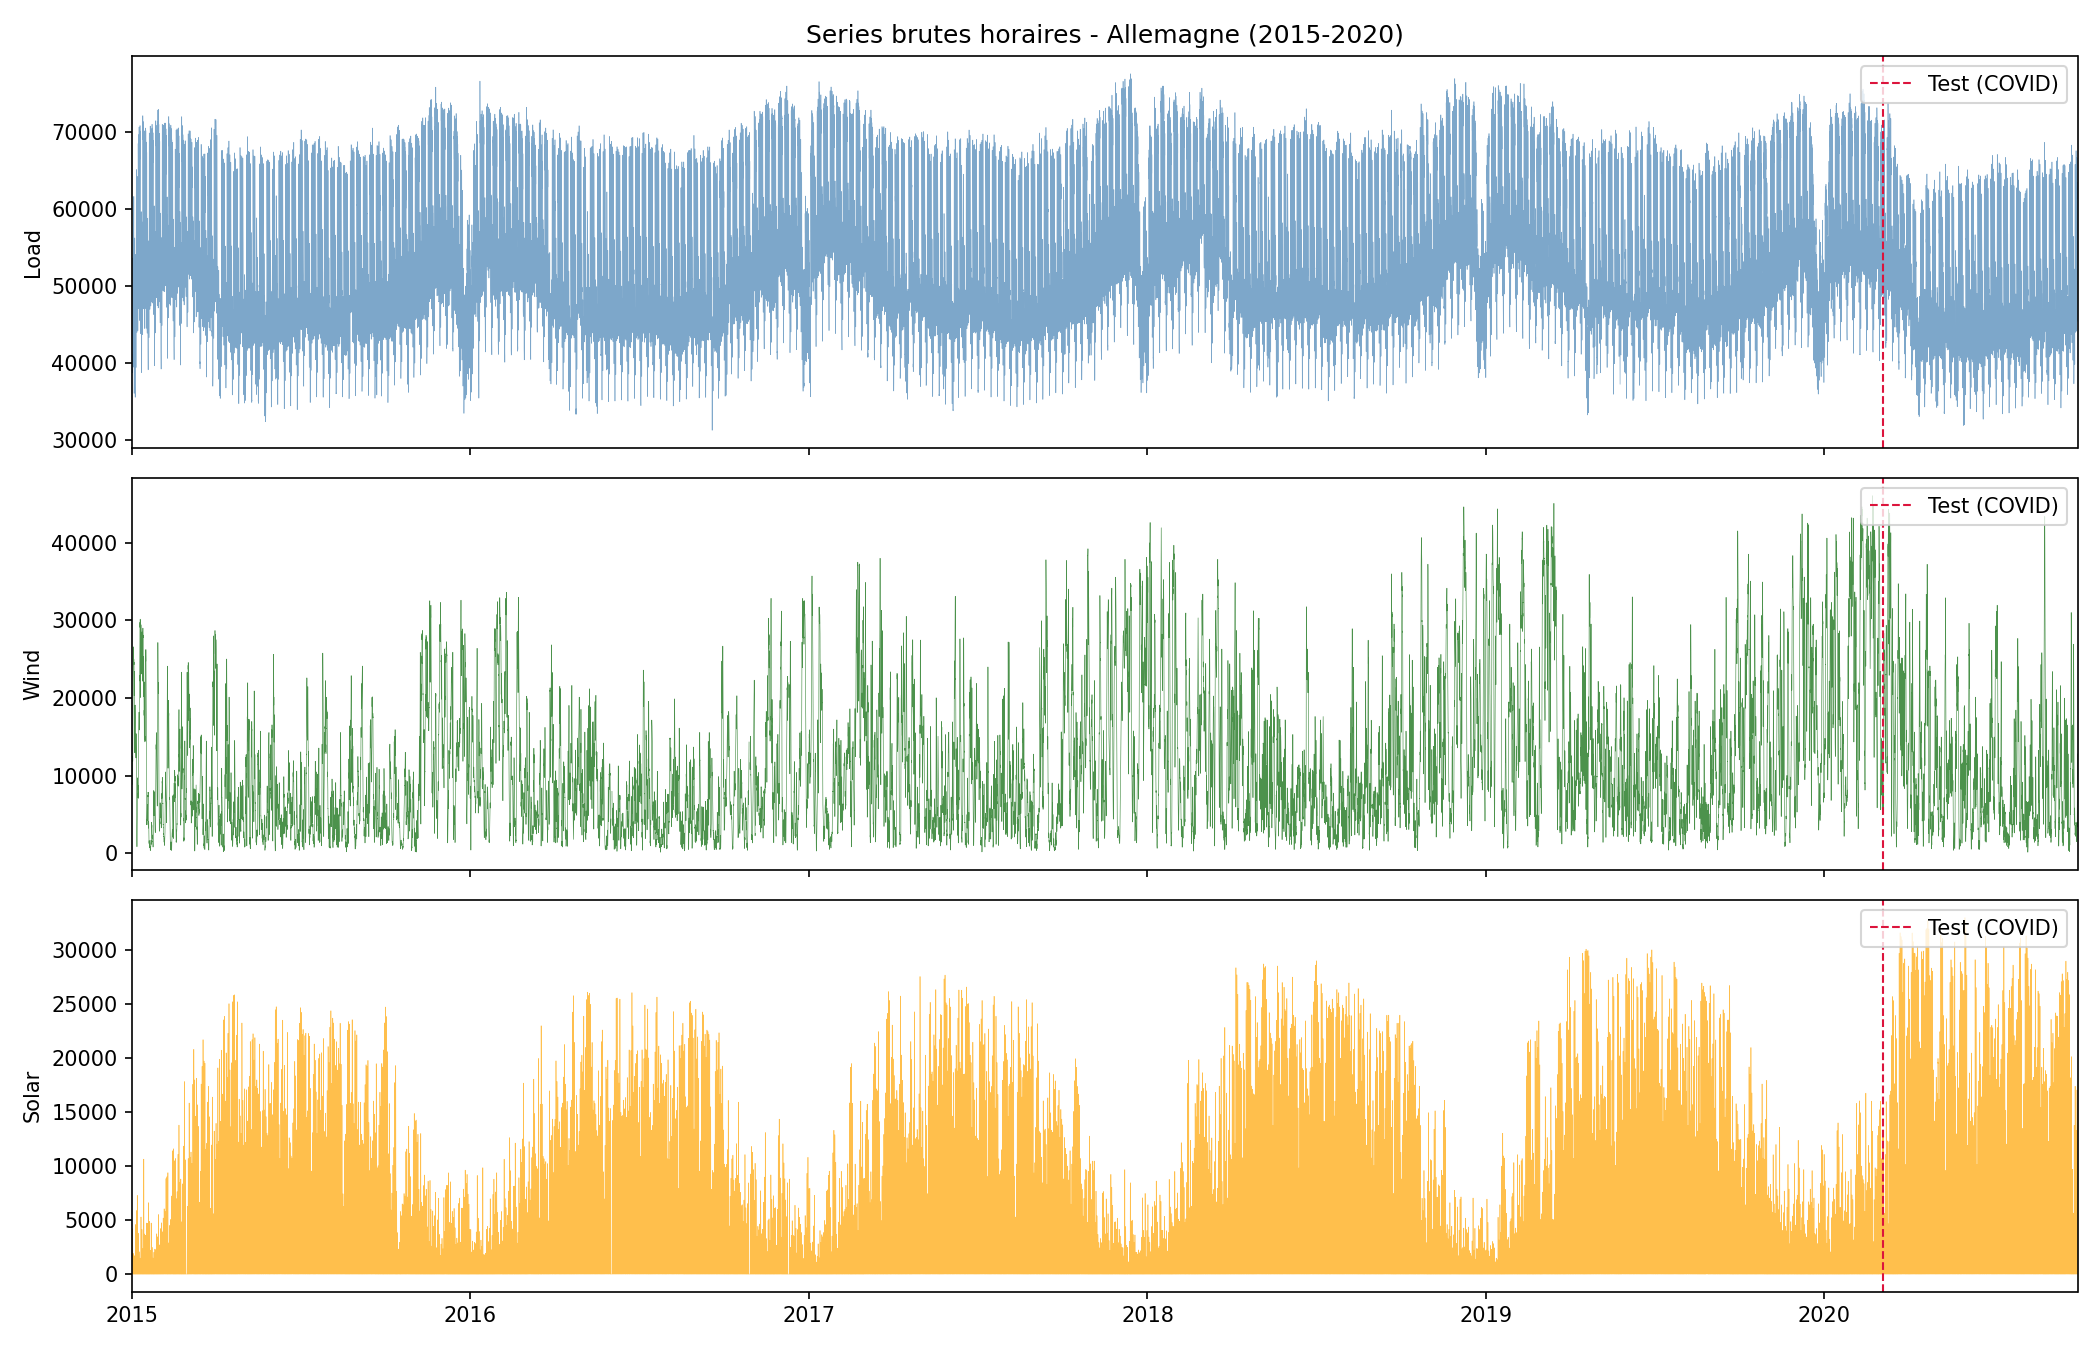
\includegraphics[width=0.95\textwidth]{py_ts_overview.png}
\caption{Vue d'ensemble des trois séries horaires (2015--2020).}
\label{fig:ts_overview}
\end{figure}

\begin{figure}[H]
\centering
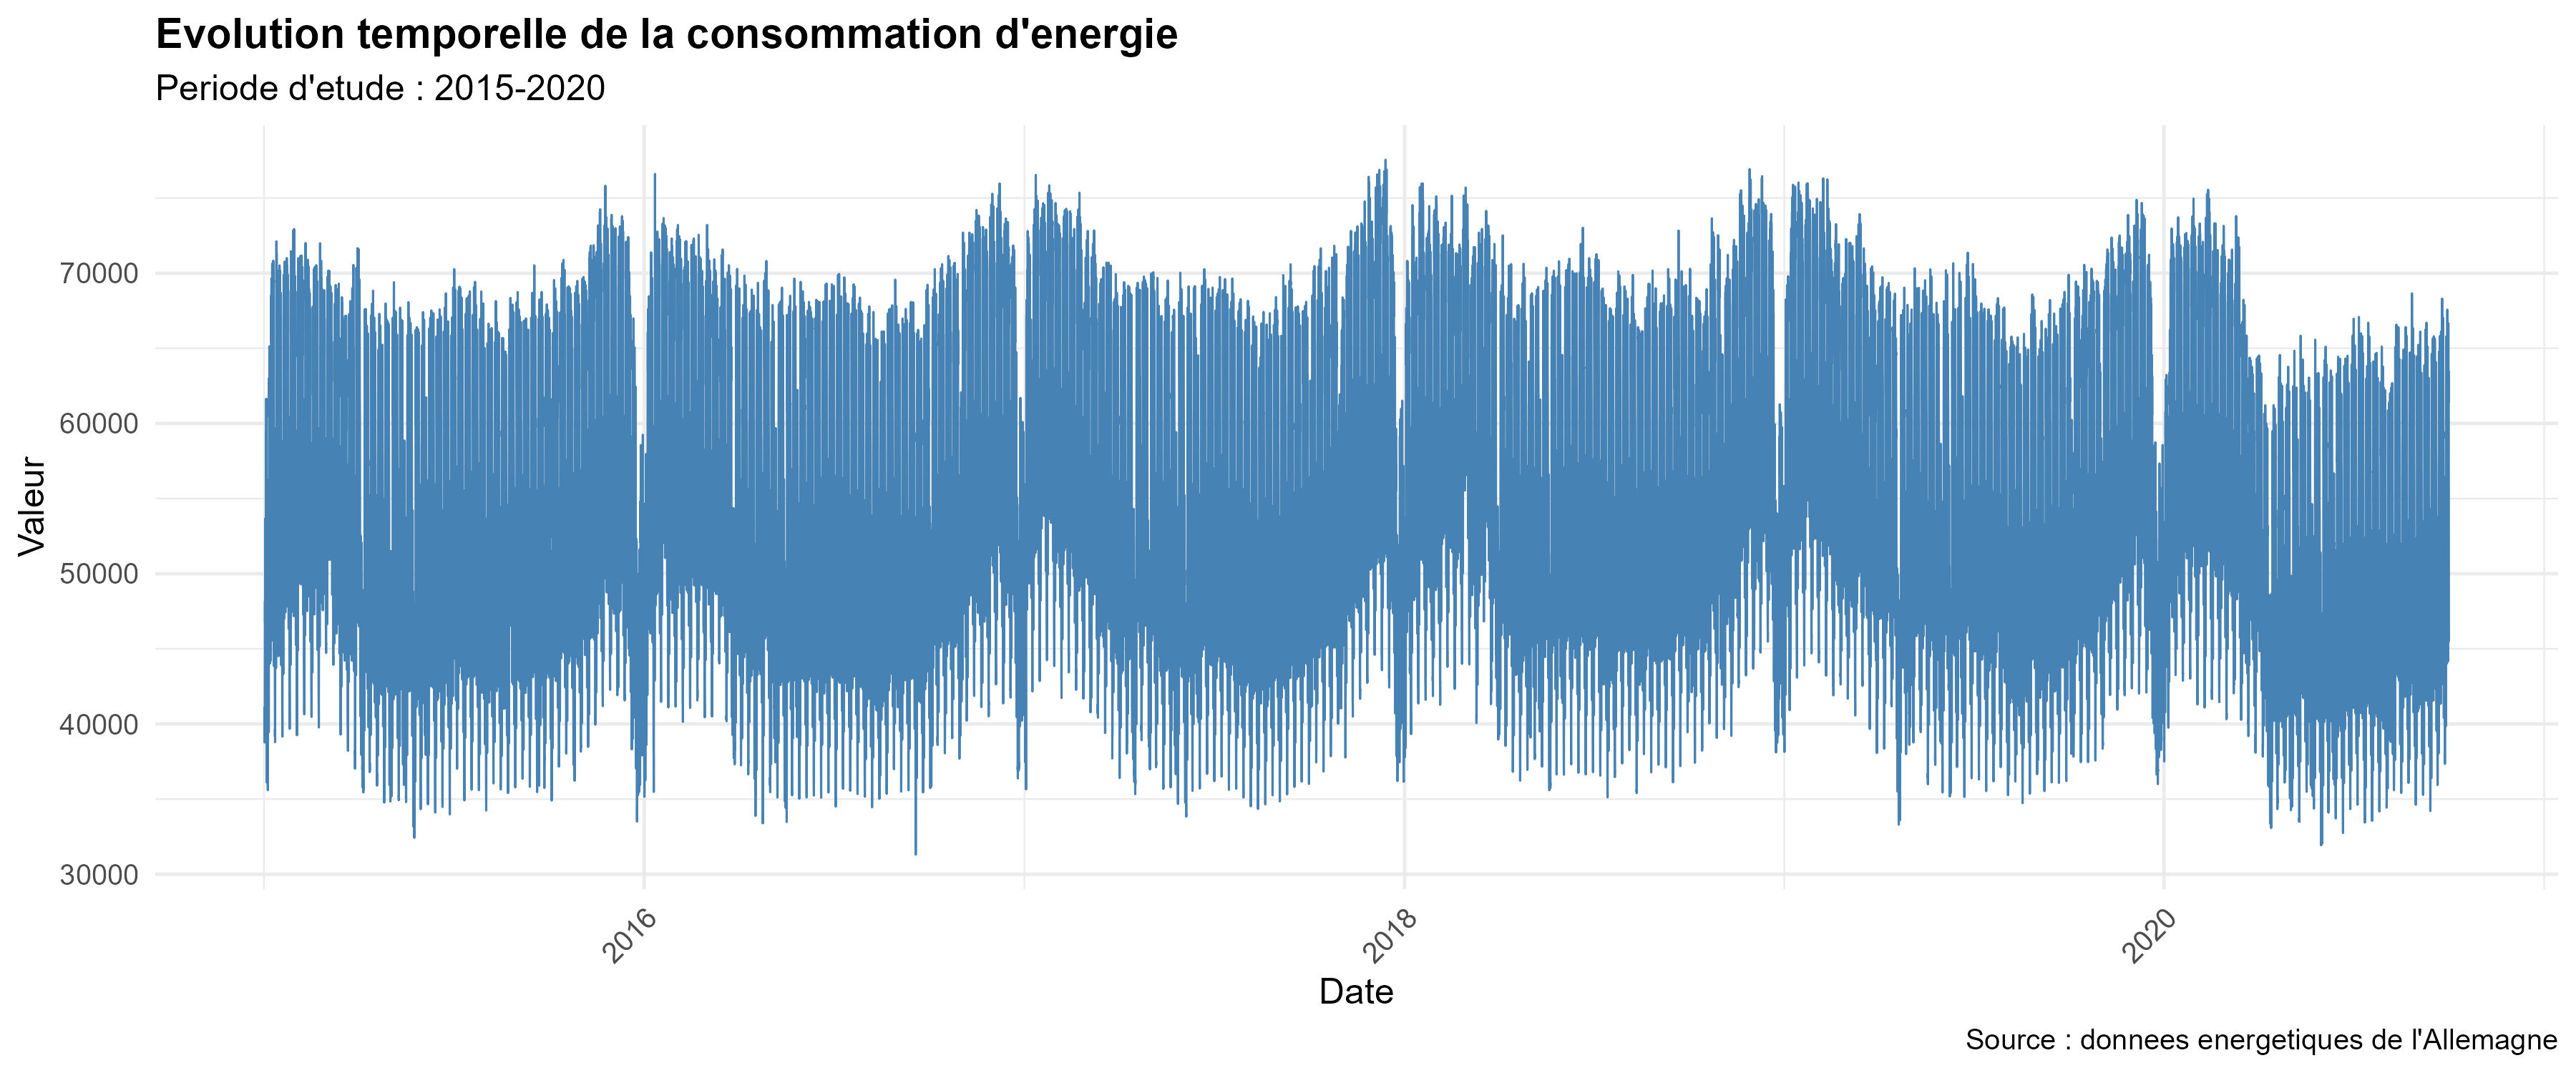
\includegraphics[width=0.9\textwidth]{Load_time_series.png}
\caption{Évolution temporelle de la consommation (\texttt{Load}).}
\label{fig:load_ts}
\end{figure}

\begin{figure}[H]
\centering
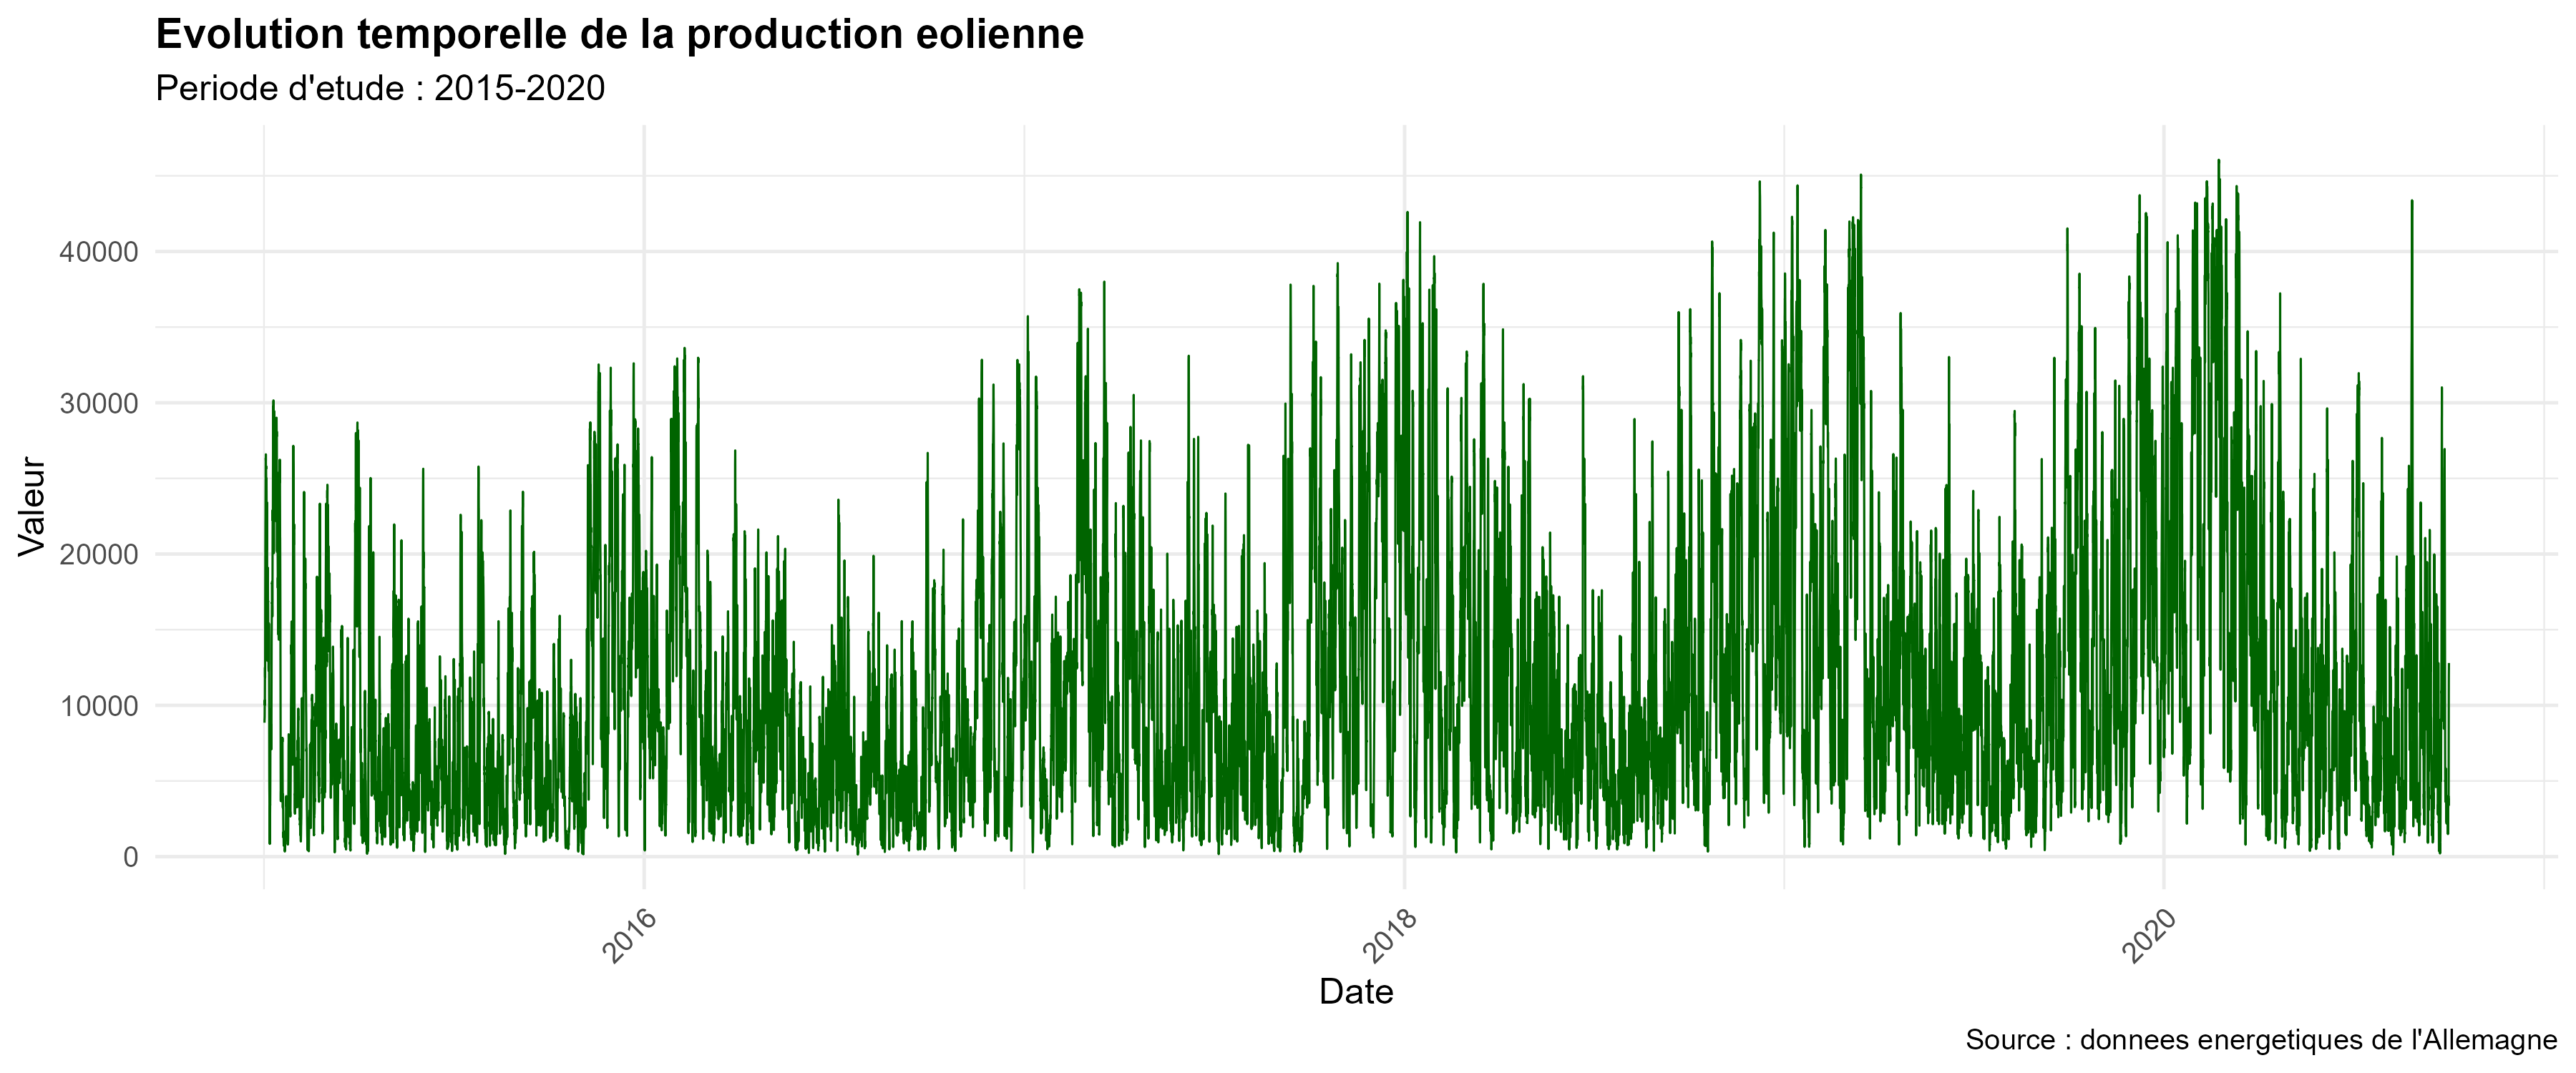
\includegraphics[width=0.9\textwidth]{Wind_time_series.png}
\caption{Évolution temporelle de la production éolienne (\texttt{Wind}).}
\label{fig:wind_ts}
\end{figure}

\begin{figure}[H]
\centering
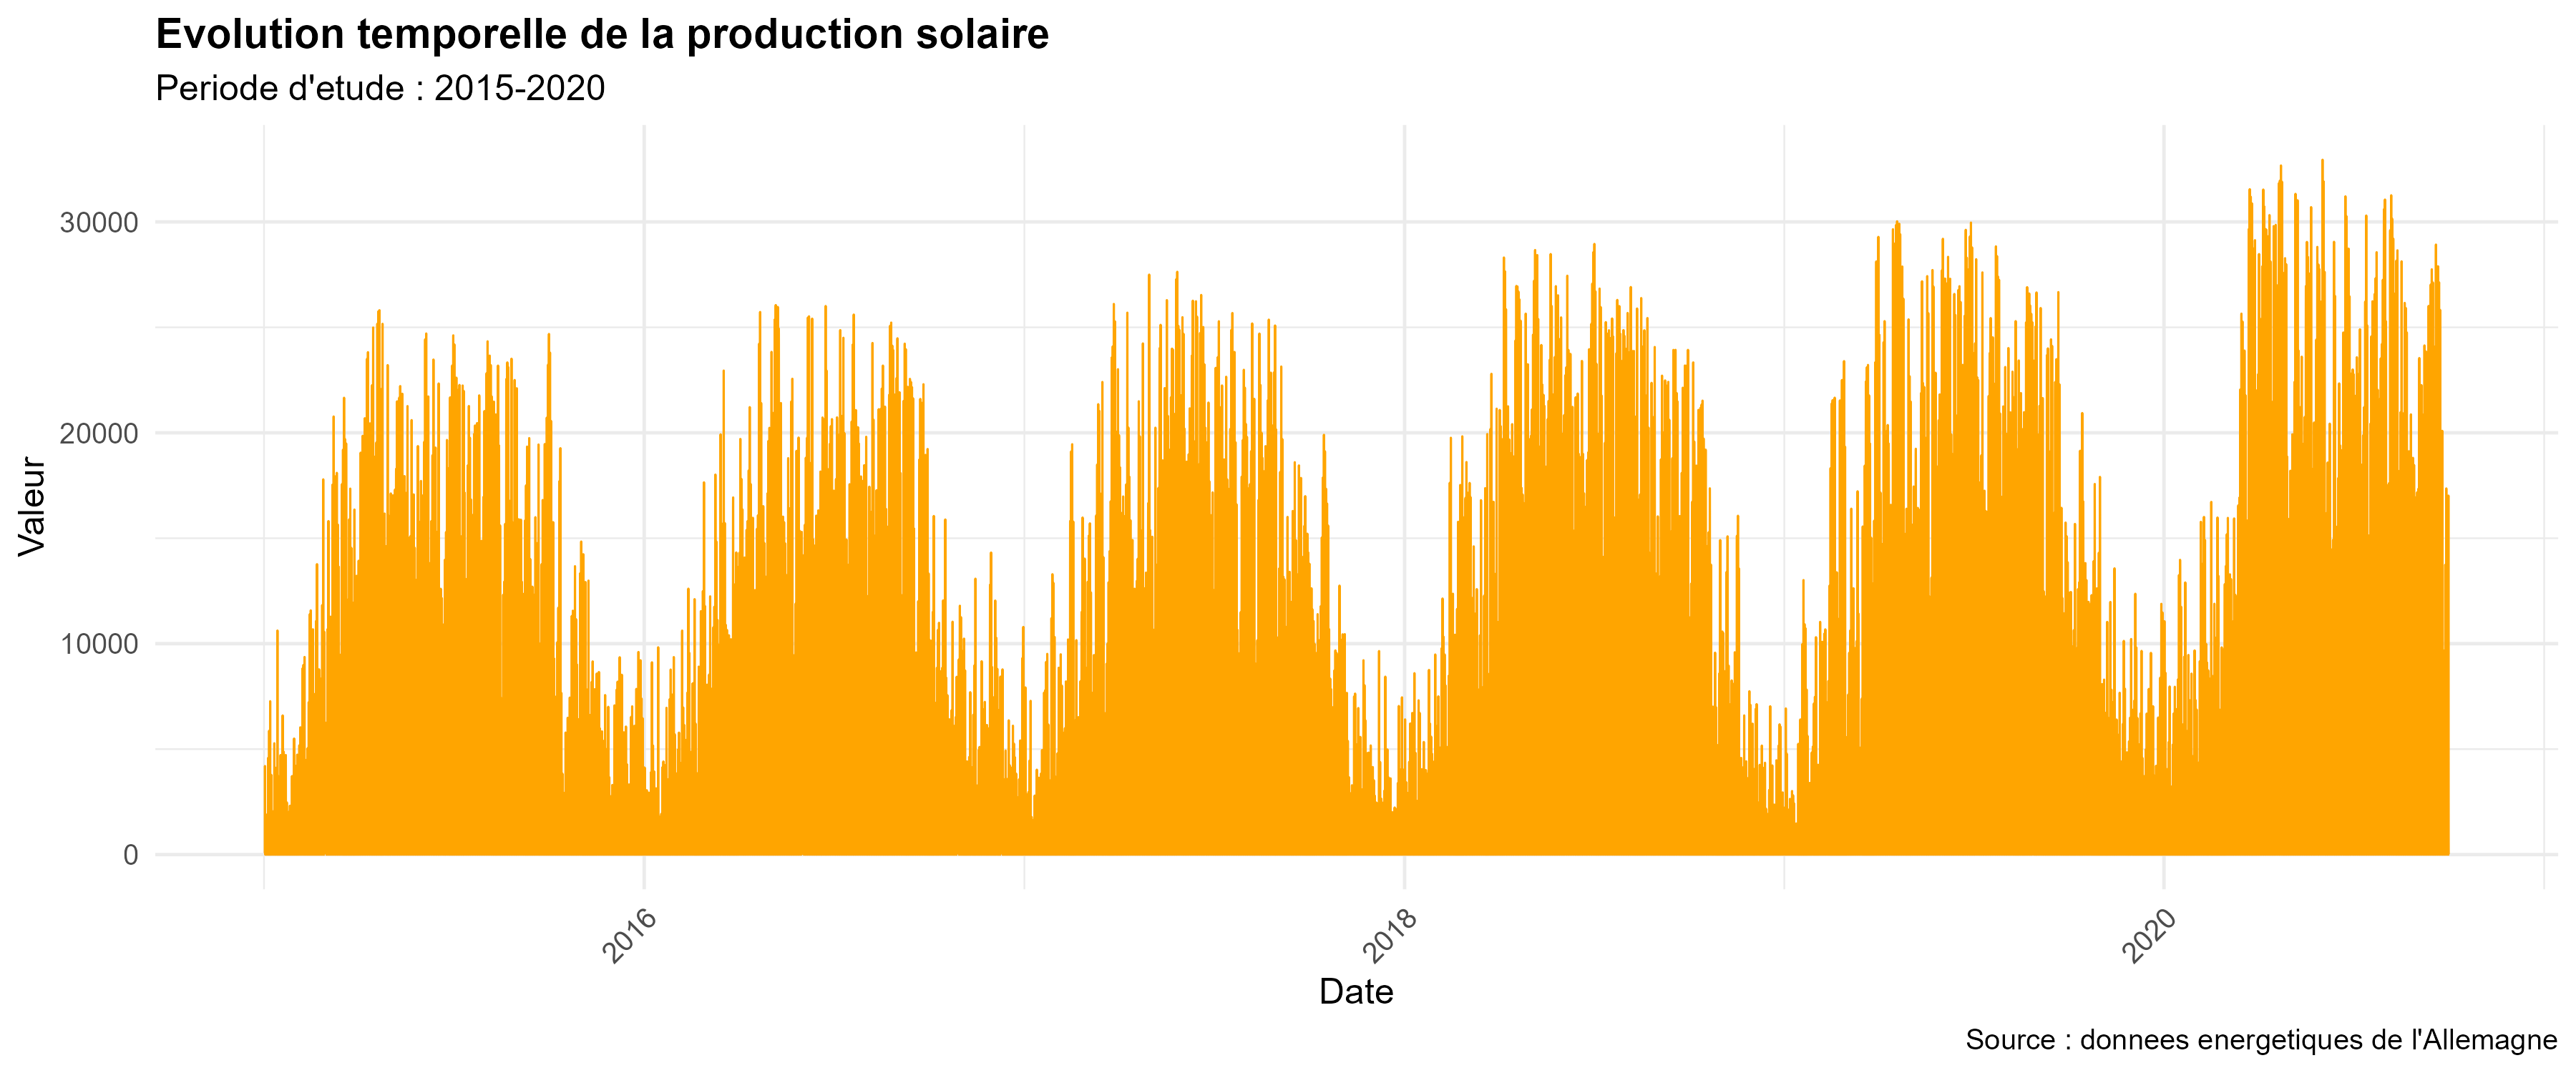
\includegraphics[width=0.9\textwidth]{Solar_time_series.png}
\caption{Évolution temporelle de la production solaire (\texttt{Solar}).}
\label{fig:solar_ts}
\end{figure}

\subsubsection{Profils saisonniers}
Le profil horaire (figure~\ref{fig:hourly}) montre un double pic de charge
(\(\approx 9\)~h et \(19\)~h) et un solaire en cloche centré sur
\(11\)--\(12\)~h. Le profil hebdomadaire (figure~\ref{fig:weekly}) révèle une
baisse de la charge le week-end, alors que la production renouvelable est
indépendante du jour de la semaine. Le profil mensuel (figure~\ref{fig:monthly})
oppose un éolien hivernal (max en décembre) à un solaire estival (max en
juin--juillet). L'évolution annuelle (figure~\ref{fig:yearly}) permet enfin de
suivre ces tendances de fond.

\begin{figure}[H]
\centering
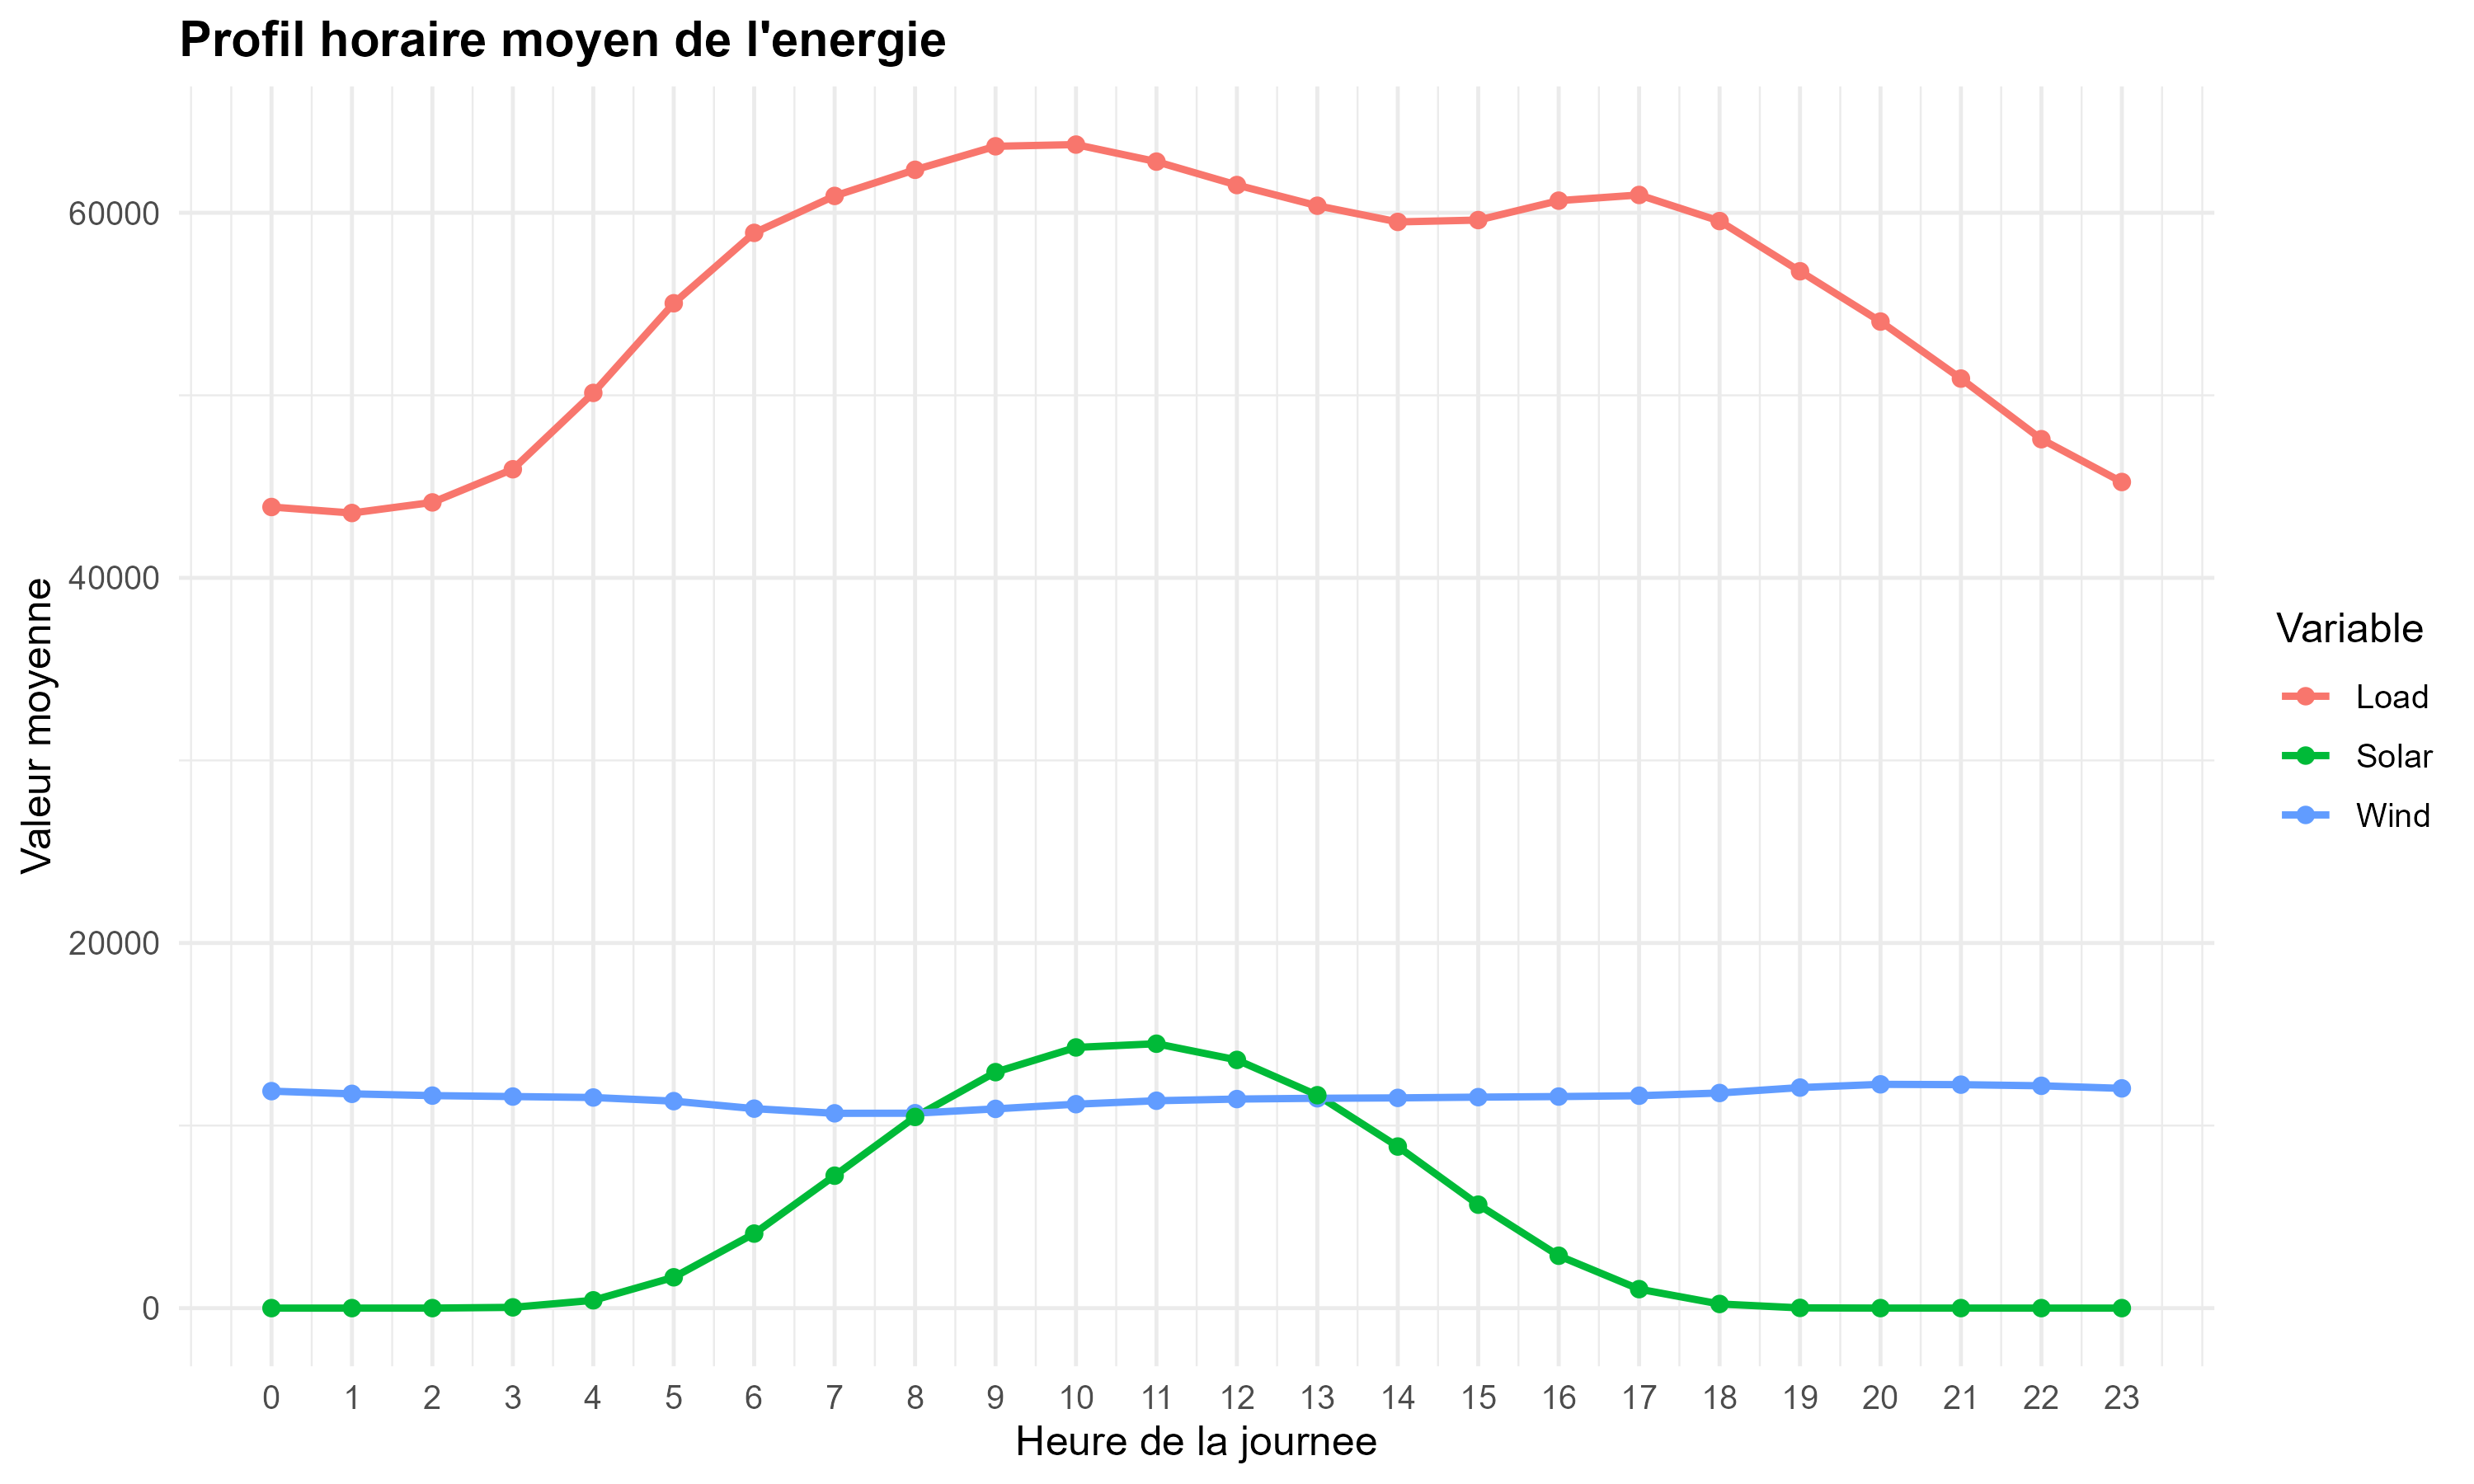
\includegraphics[width=0.85\textwidth]{hourly_profiles.png}
\caption{Profil horaire moyen des trois séries.}
\label{fig:hourly}
\end{figure}

\begin{figure}[H]
\centering
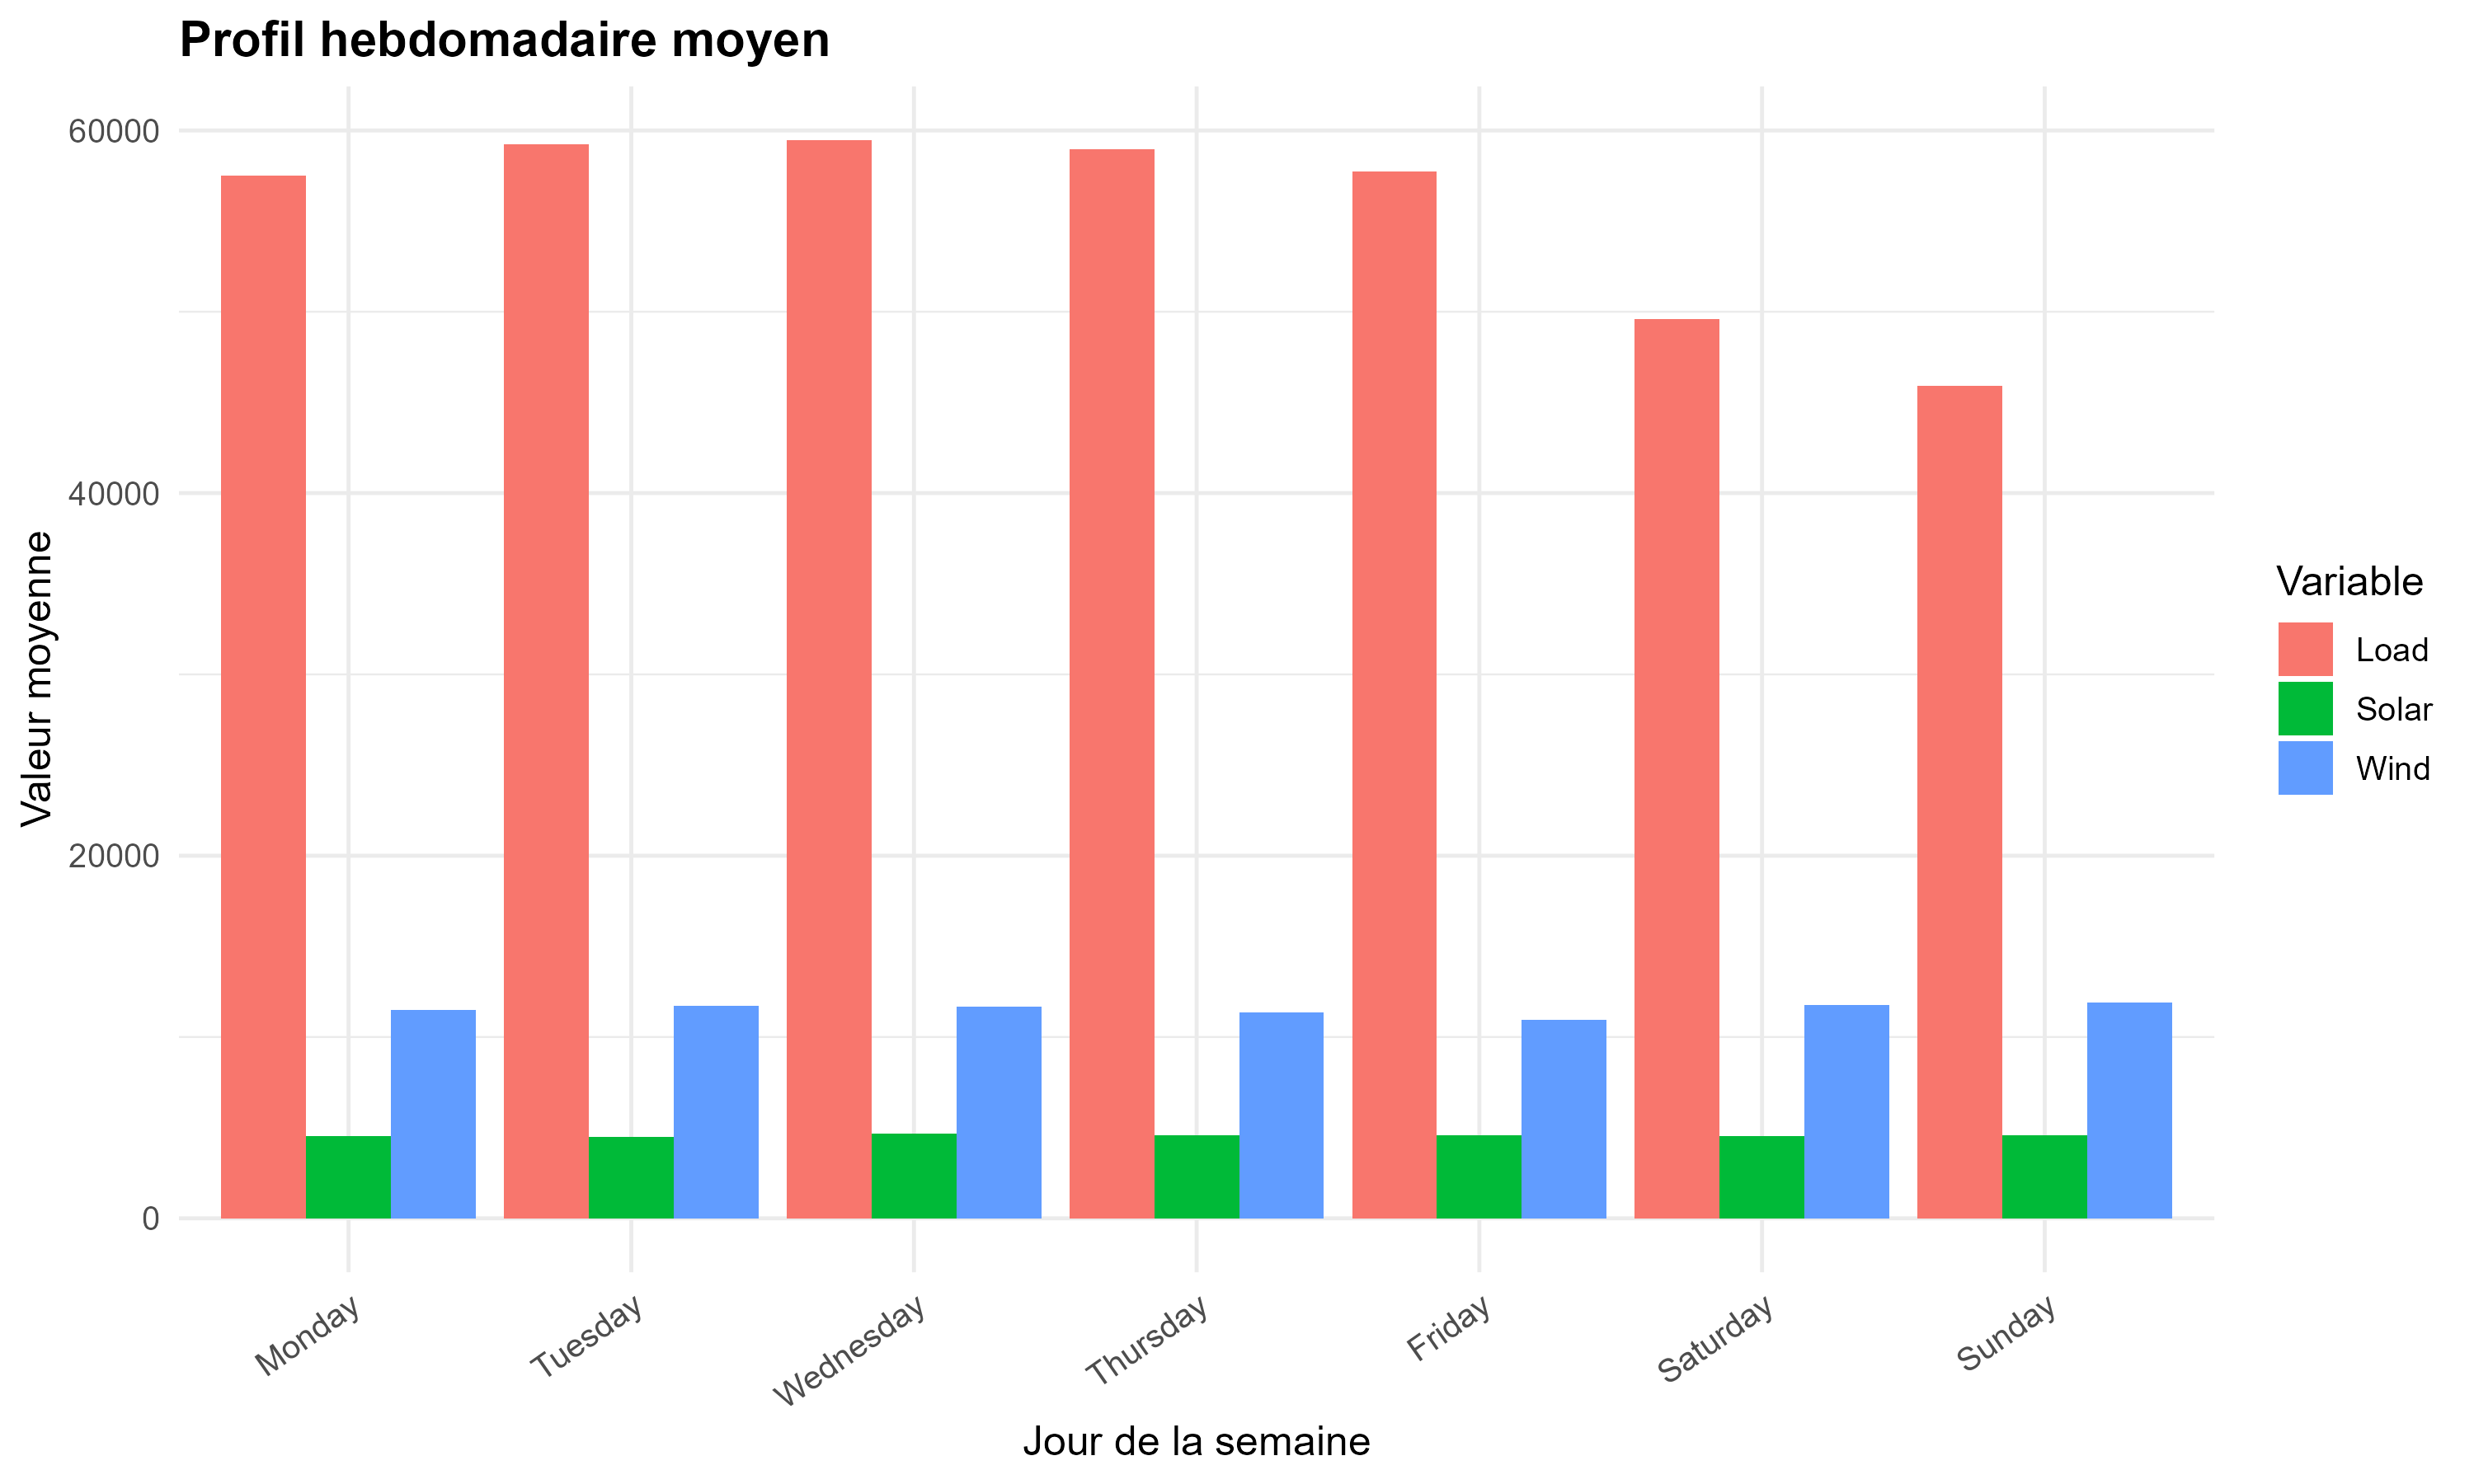
\includegraphics[width=0.85\textwidth]{weekly_profiles.png}
\caption{Profil hebdomadaire moyen.}
\label{fig:weekly}
\end{figure}

\begin{figure}[H]
\centering
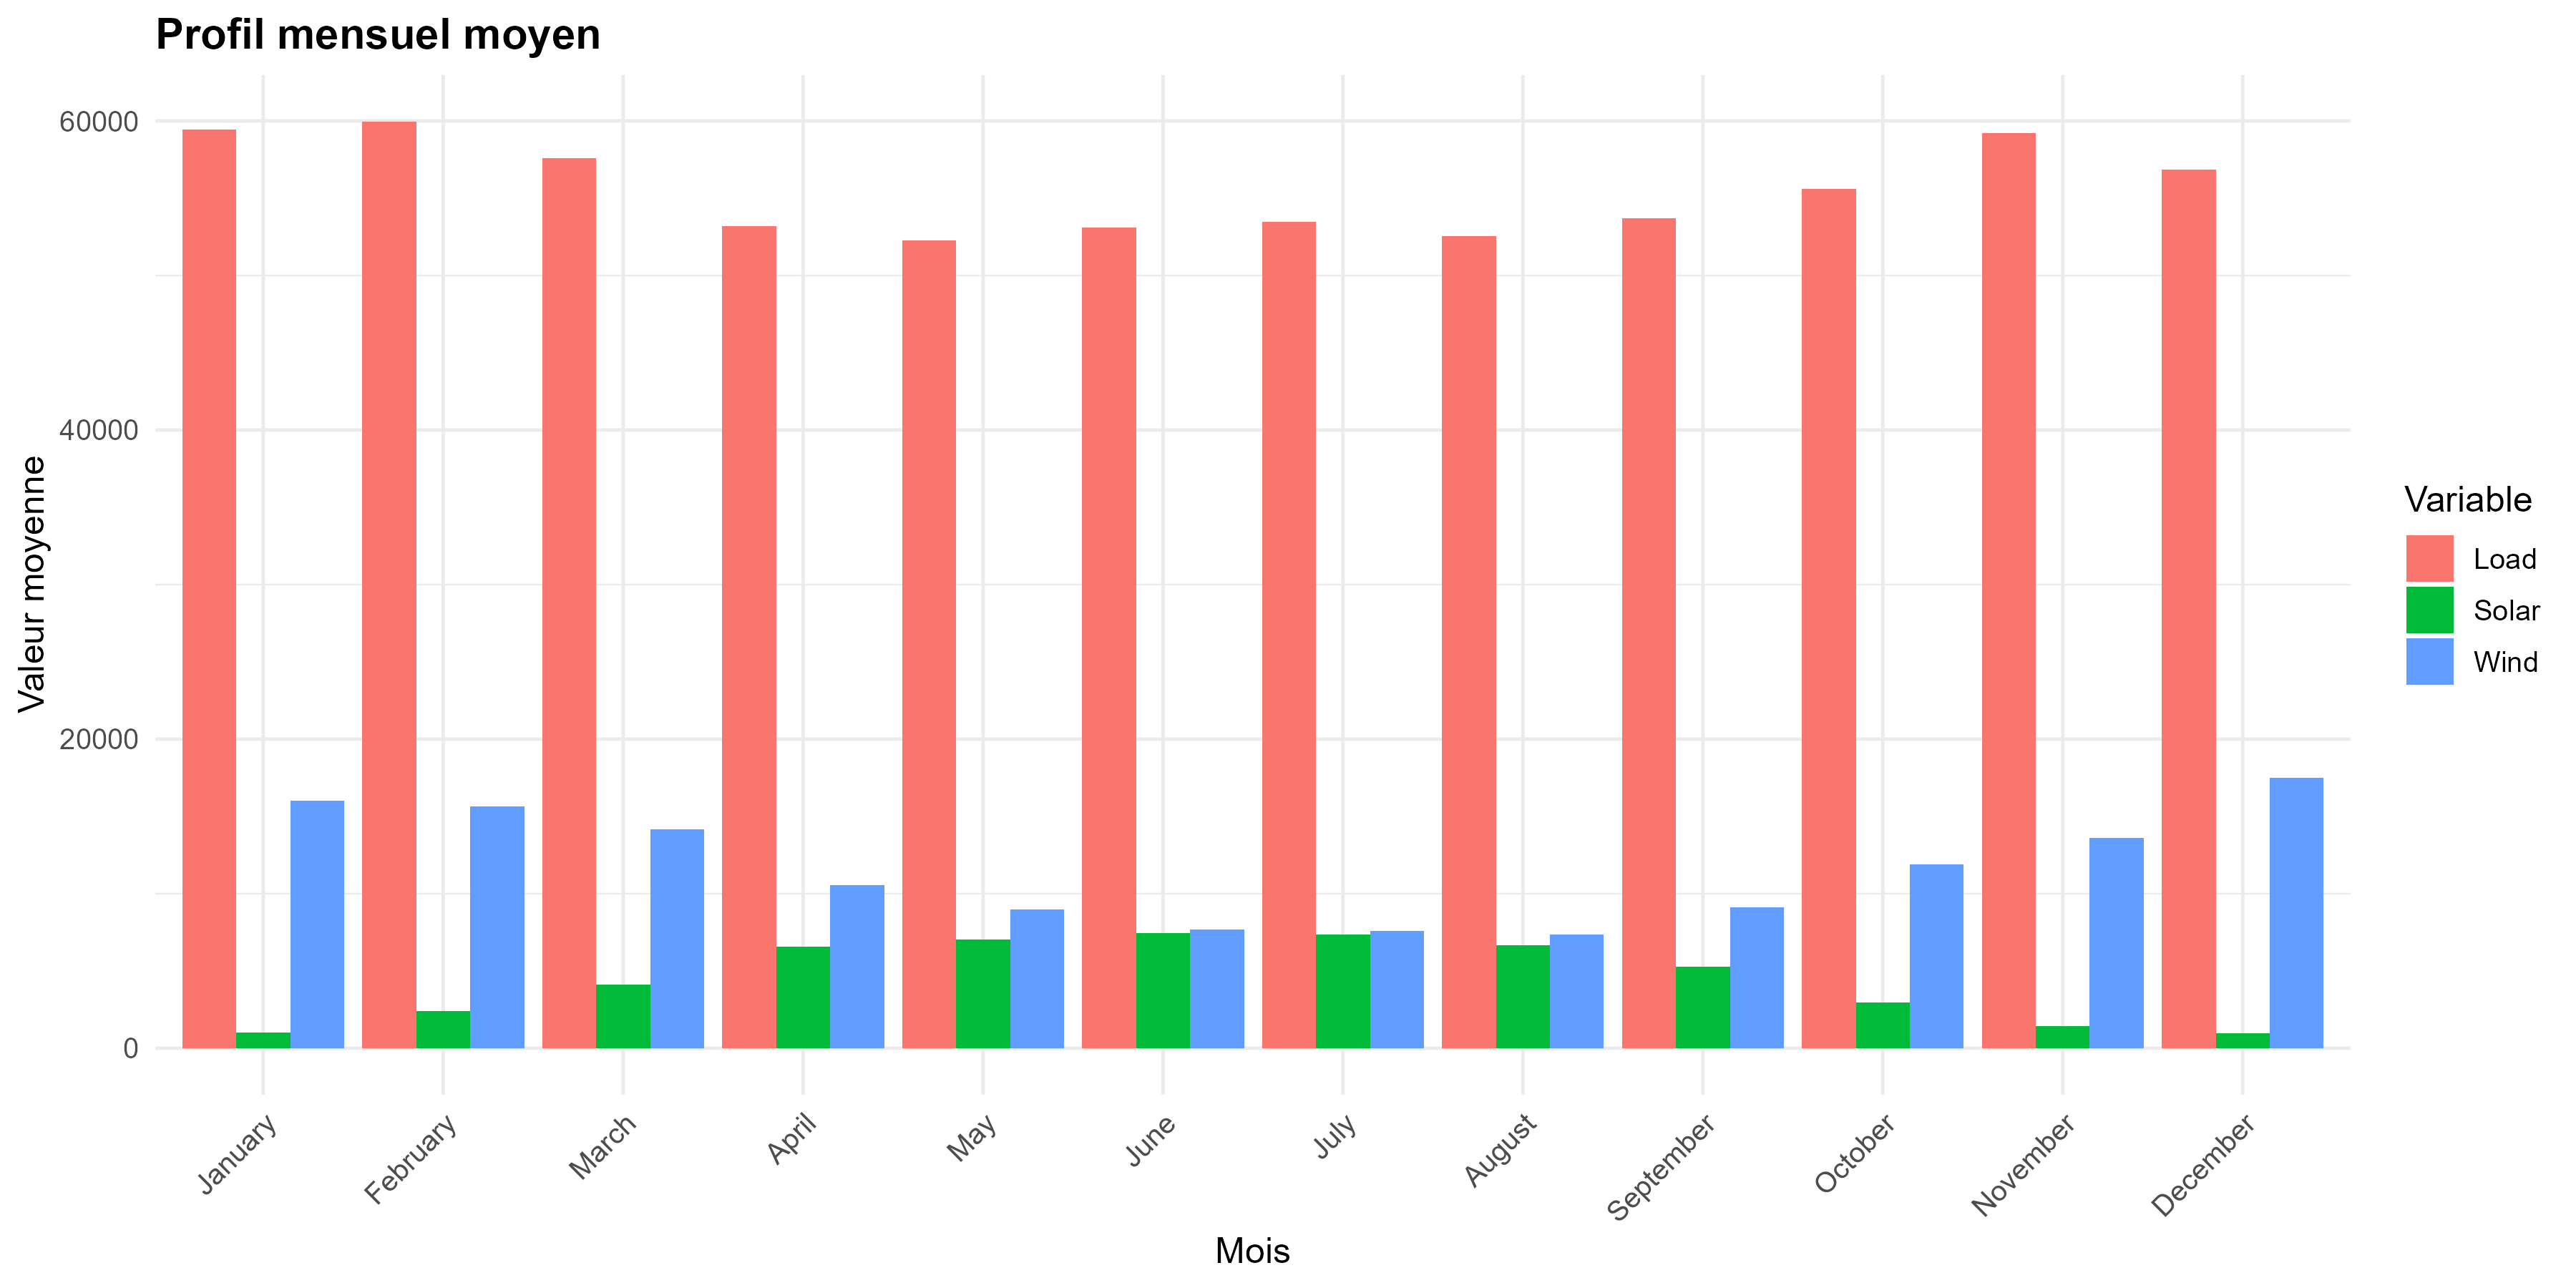
\includegraphics[width=0.9\textwidth]{monthly_profiles.png}
\caption{Profil mensuel moyen.}
\label{fig:monthly}
\end{figure}

\begin{figure}[H]
\centering
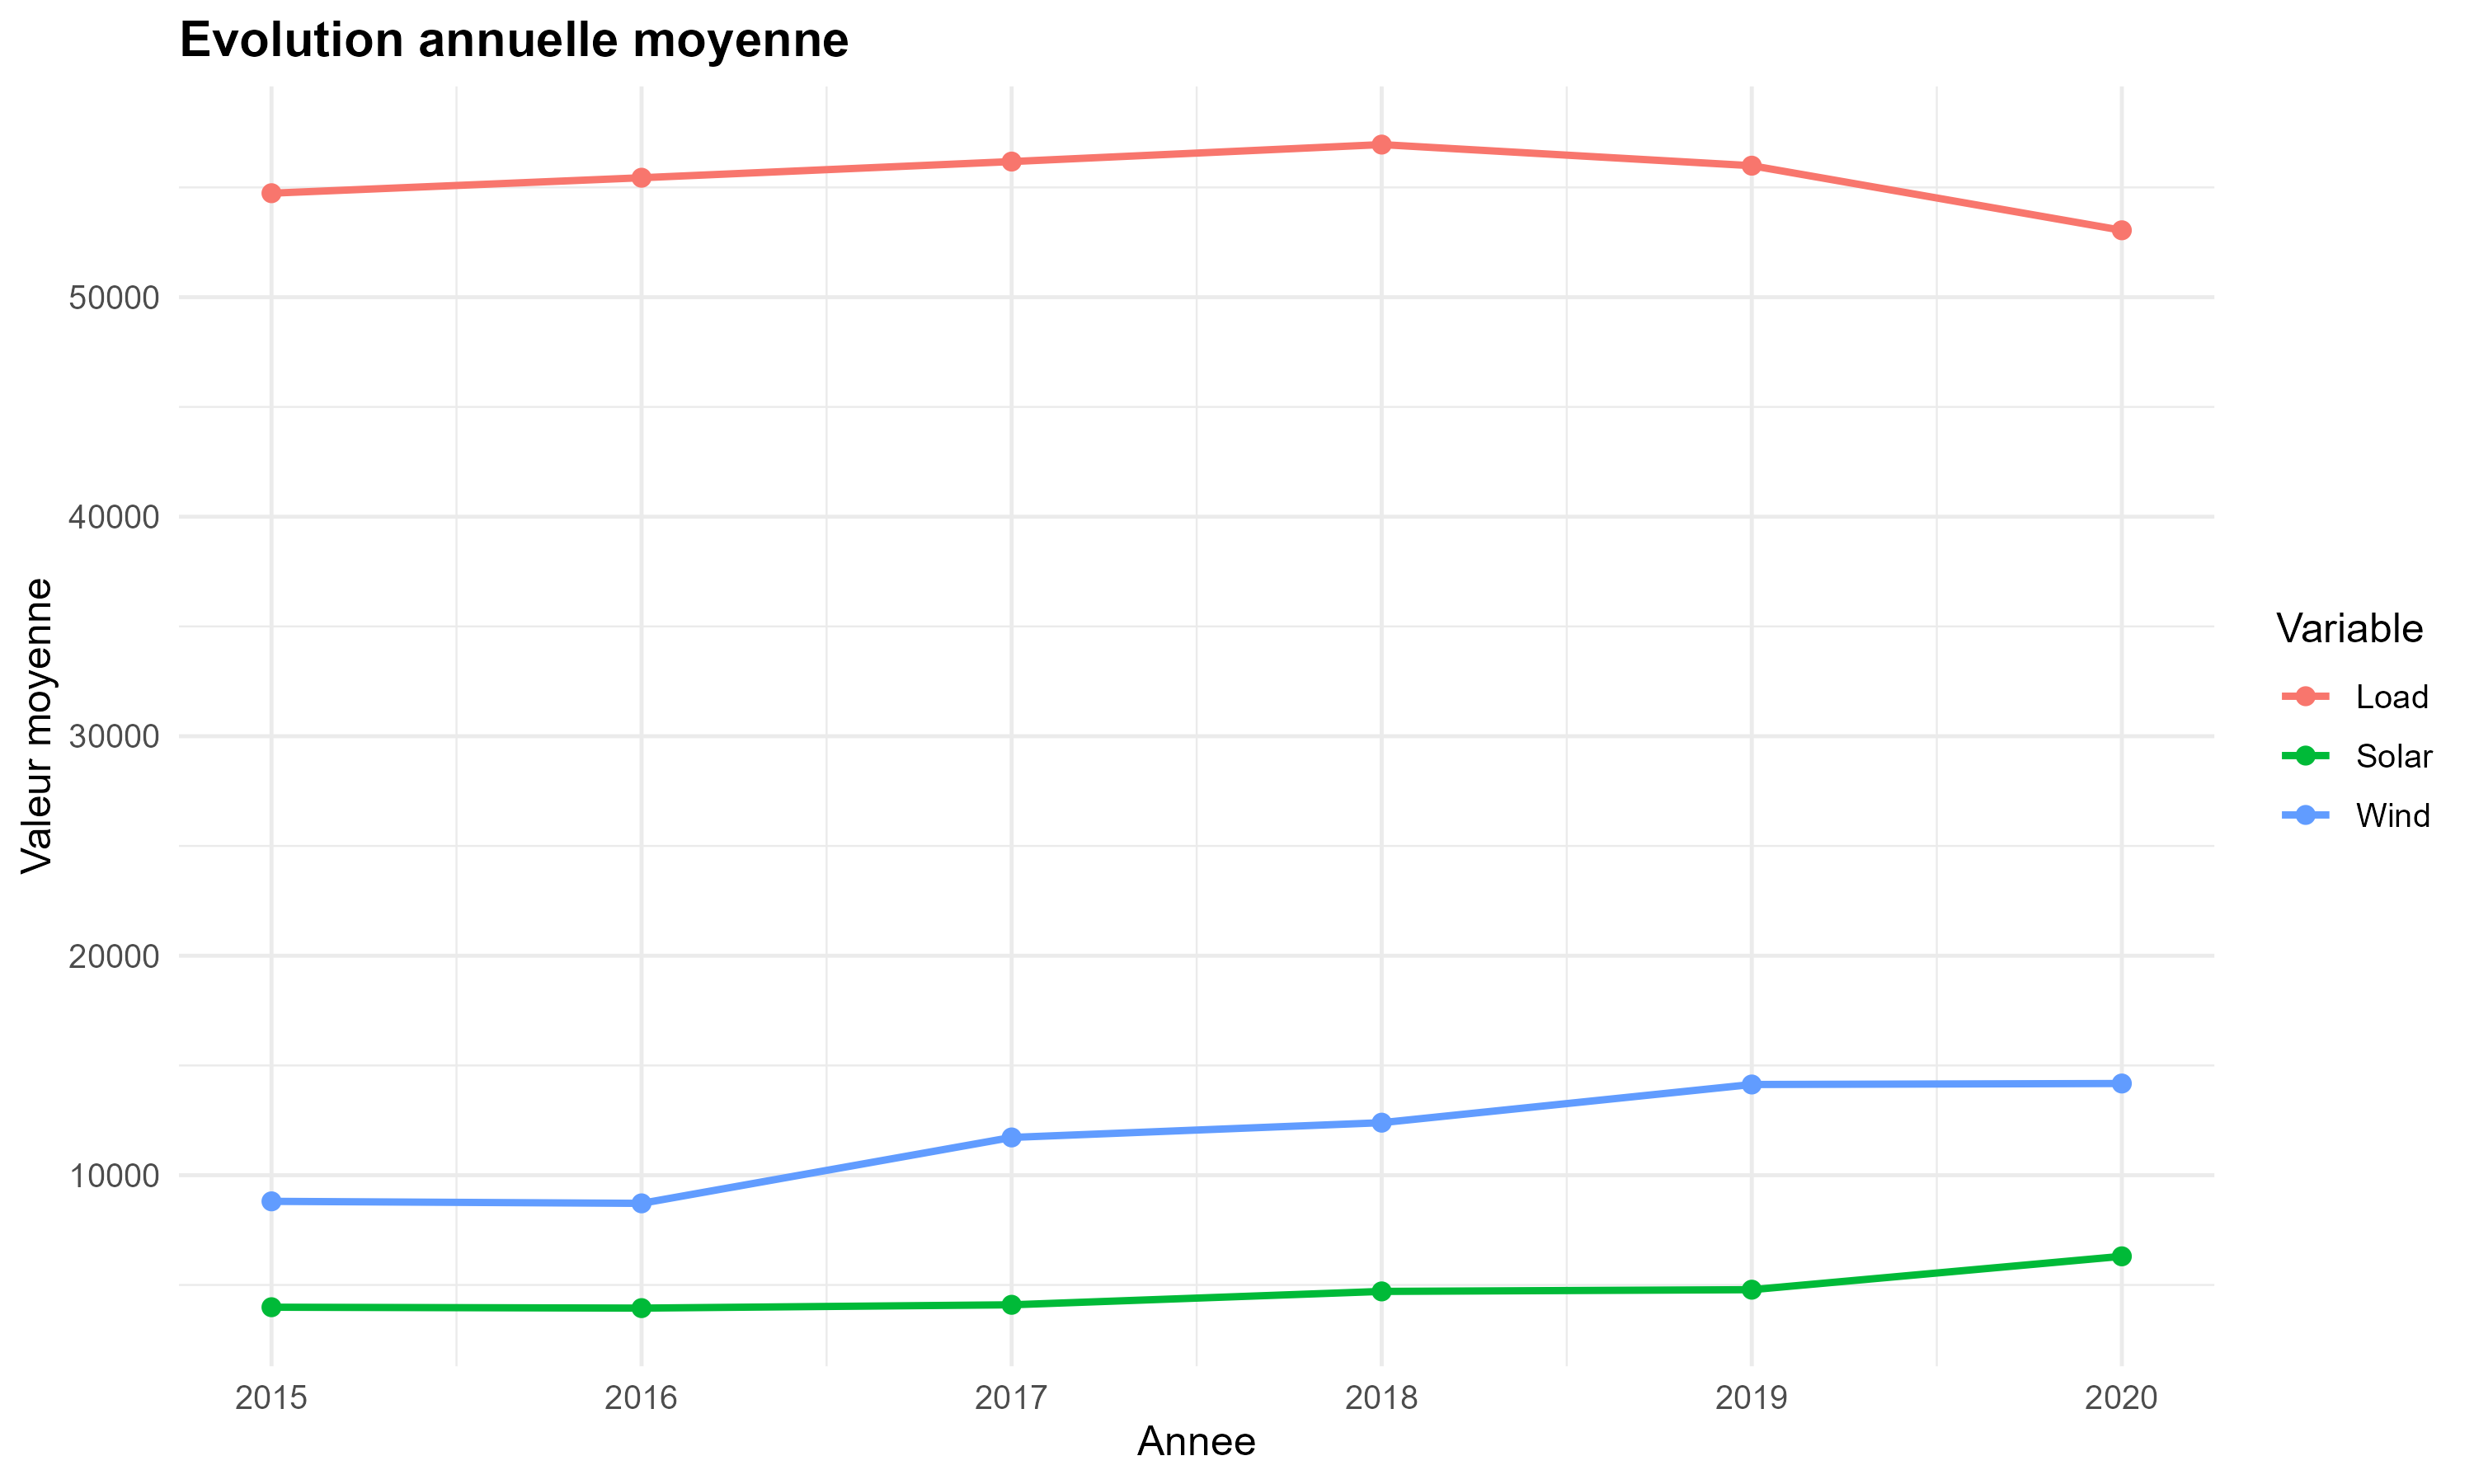
\includegraphics[width=0.8\textwidth]{yearly_profiles.png}
\caption{Évolution annuelle moyenne.}
\label{fig:yearly}
\end{figure}

\begin{figure}[H]
\centering
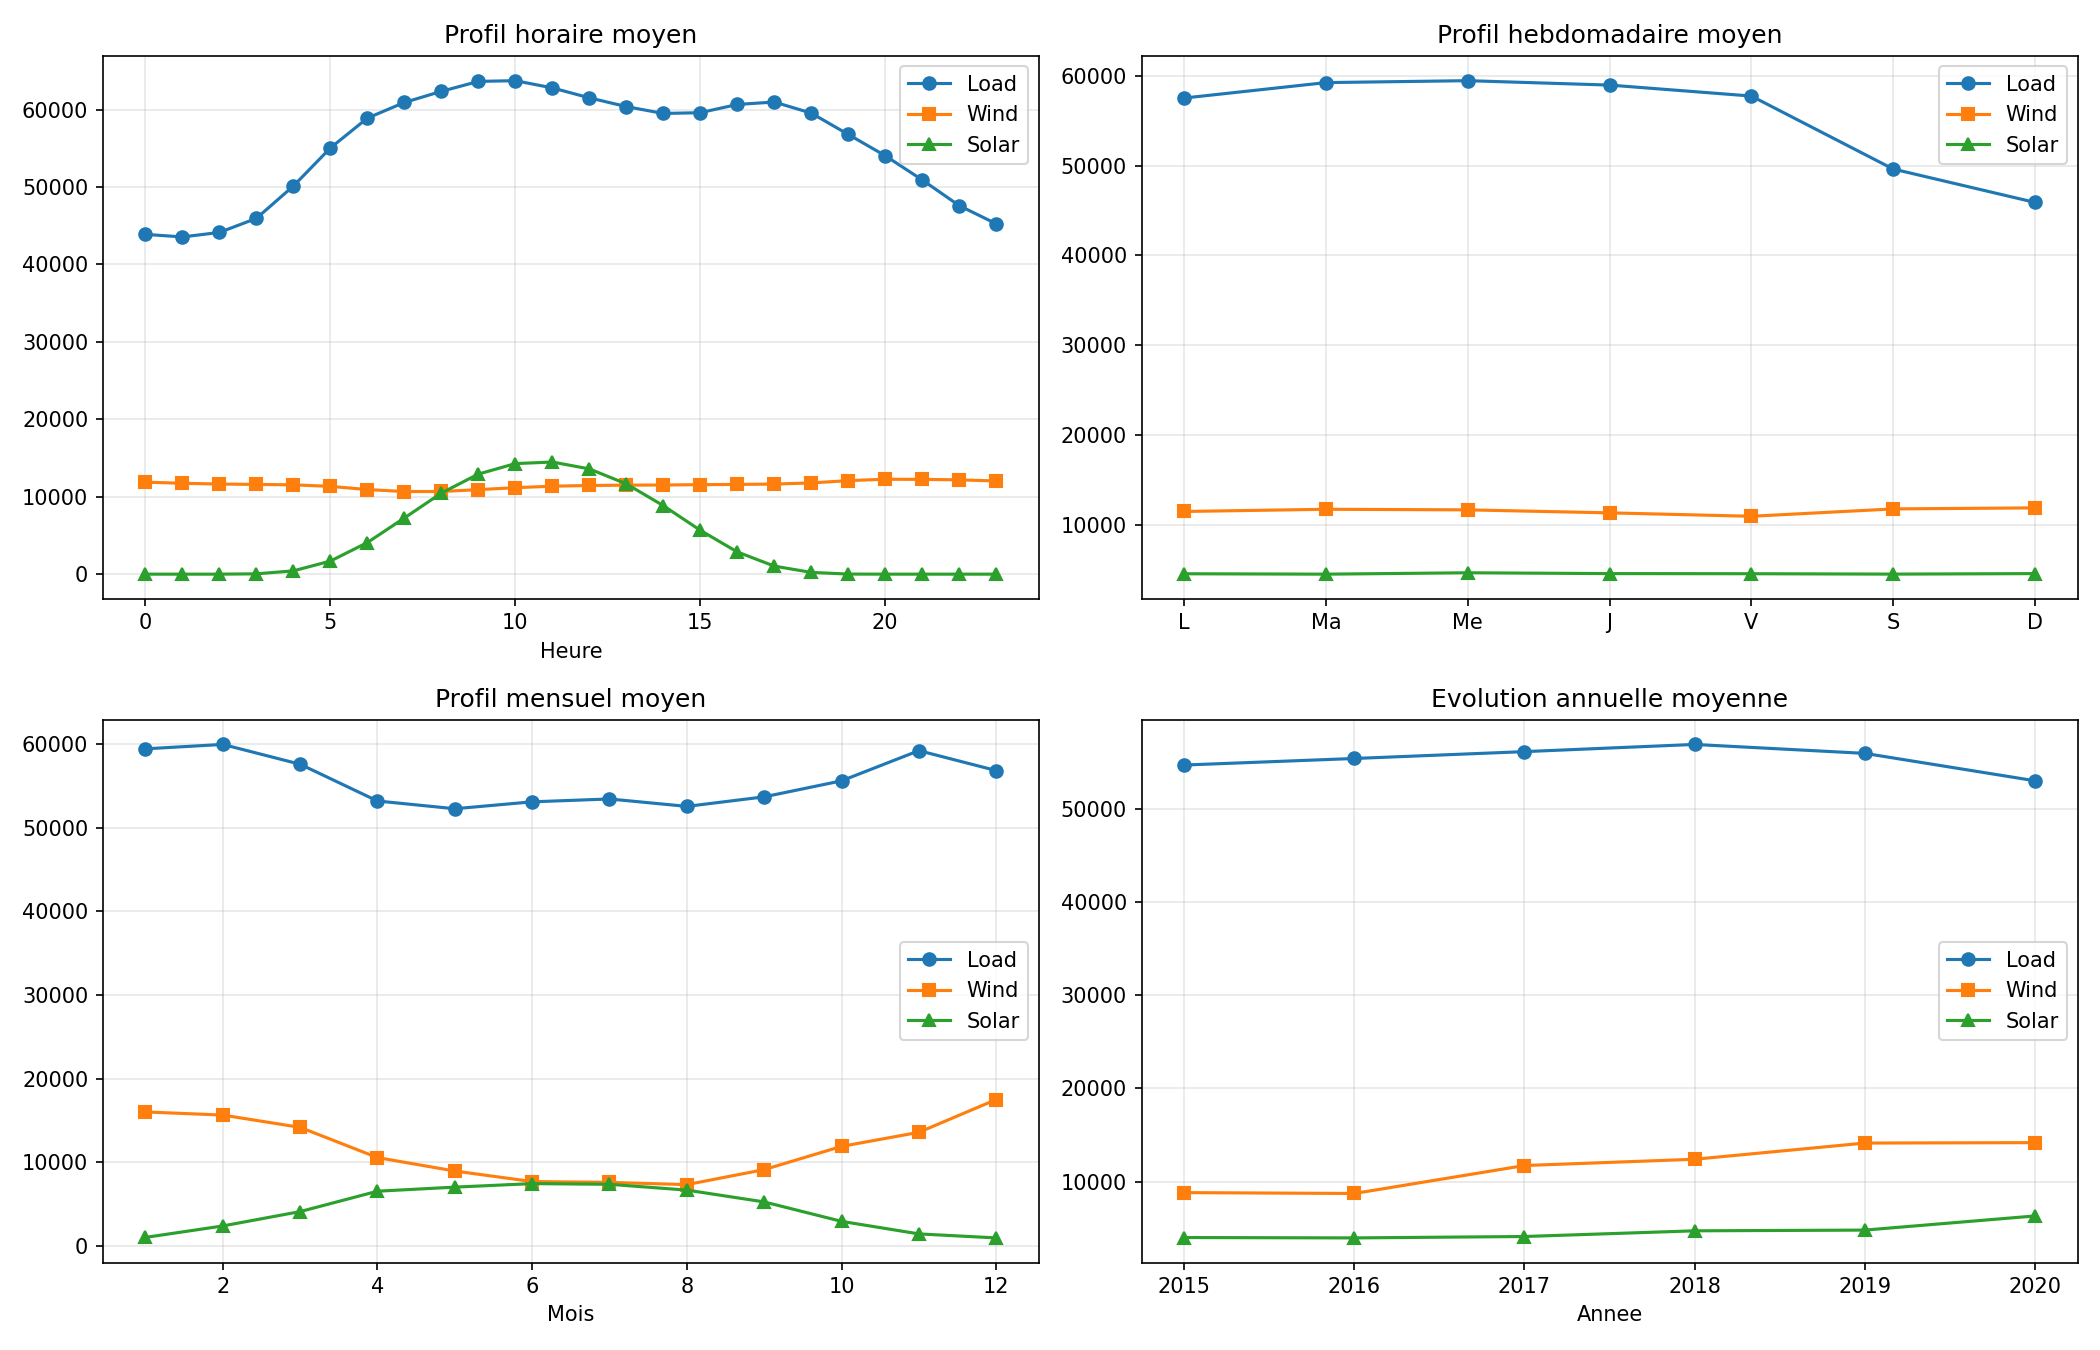
\includegraphics[width=0.9\textwidth]{py_seasonal_profiles.png}
\caption{Profils saisonniers (calcul Python).}
\label{fig:seasonal}
\end{figure}

\begin{figure}[H]
\centering
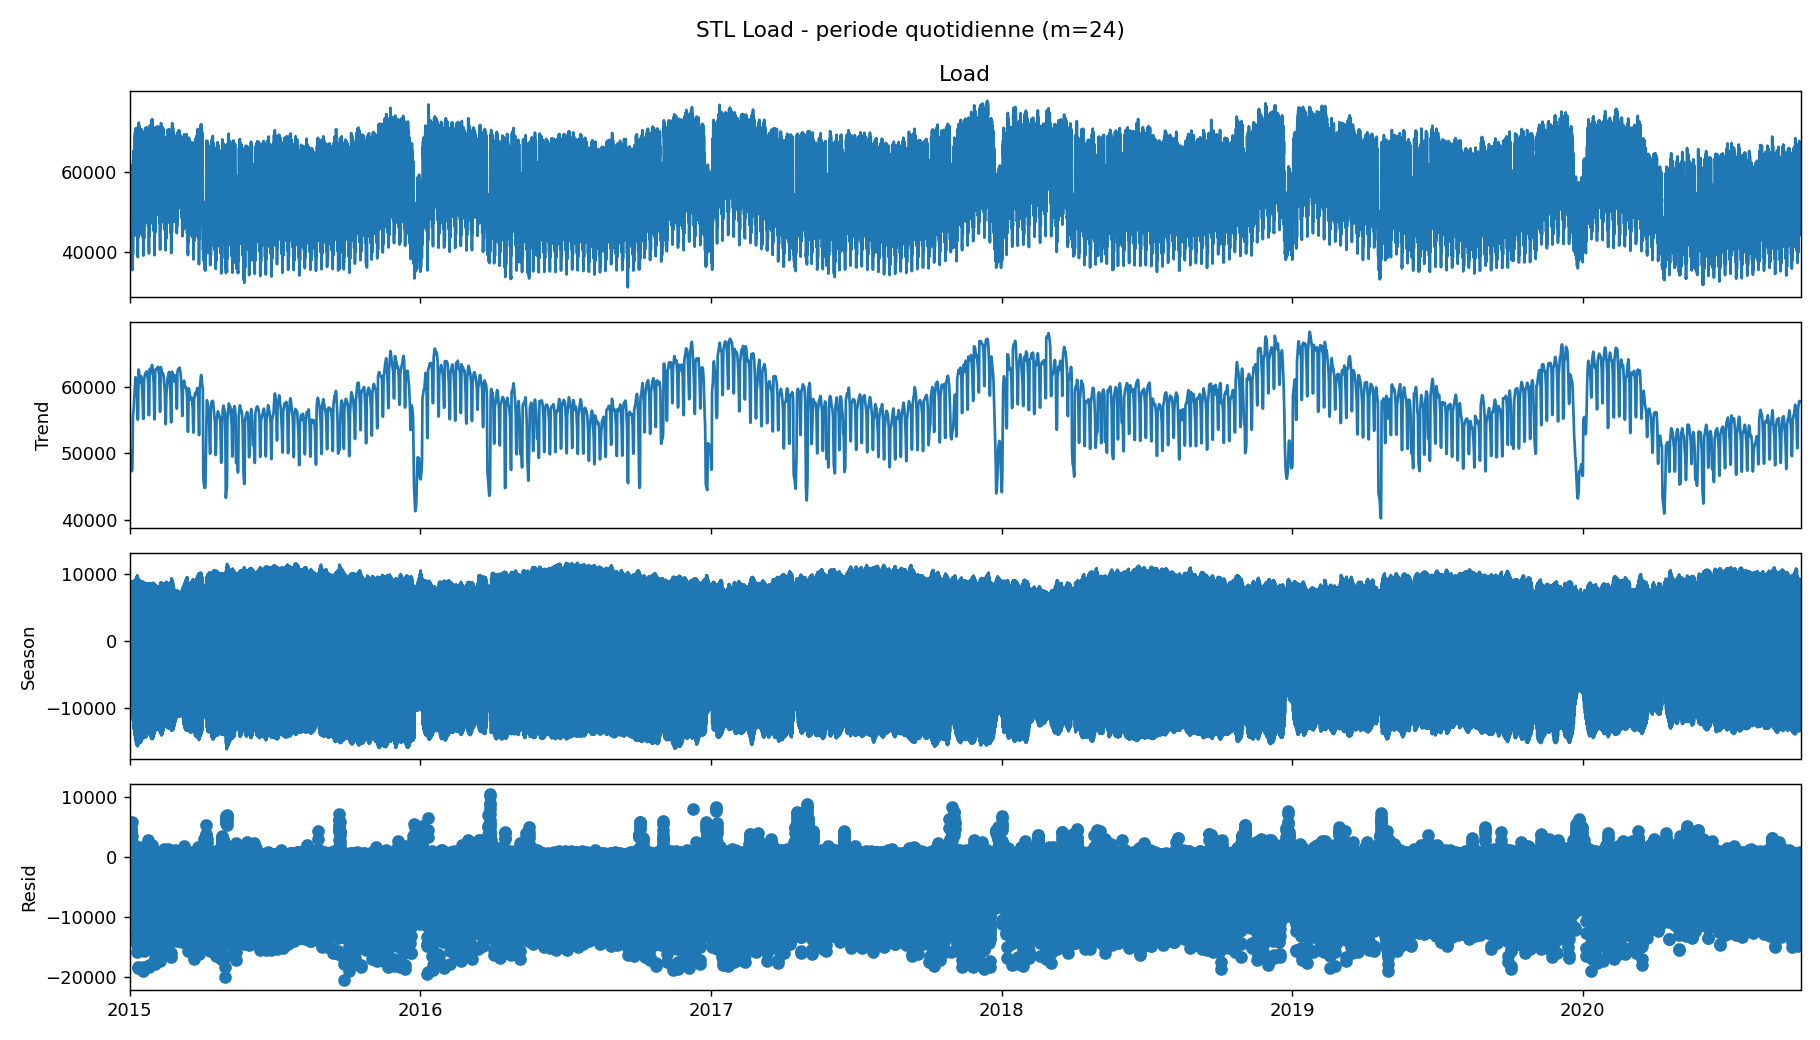
\includegraphics[width=0.75\textwidth]{py_stl_load_daily.png}
\caption{Décomposition STL de la charge (cycle journalier).}
\label{fig:stl_daily}
\end{figure}

\begin{figure}[H]
\centering
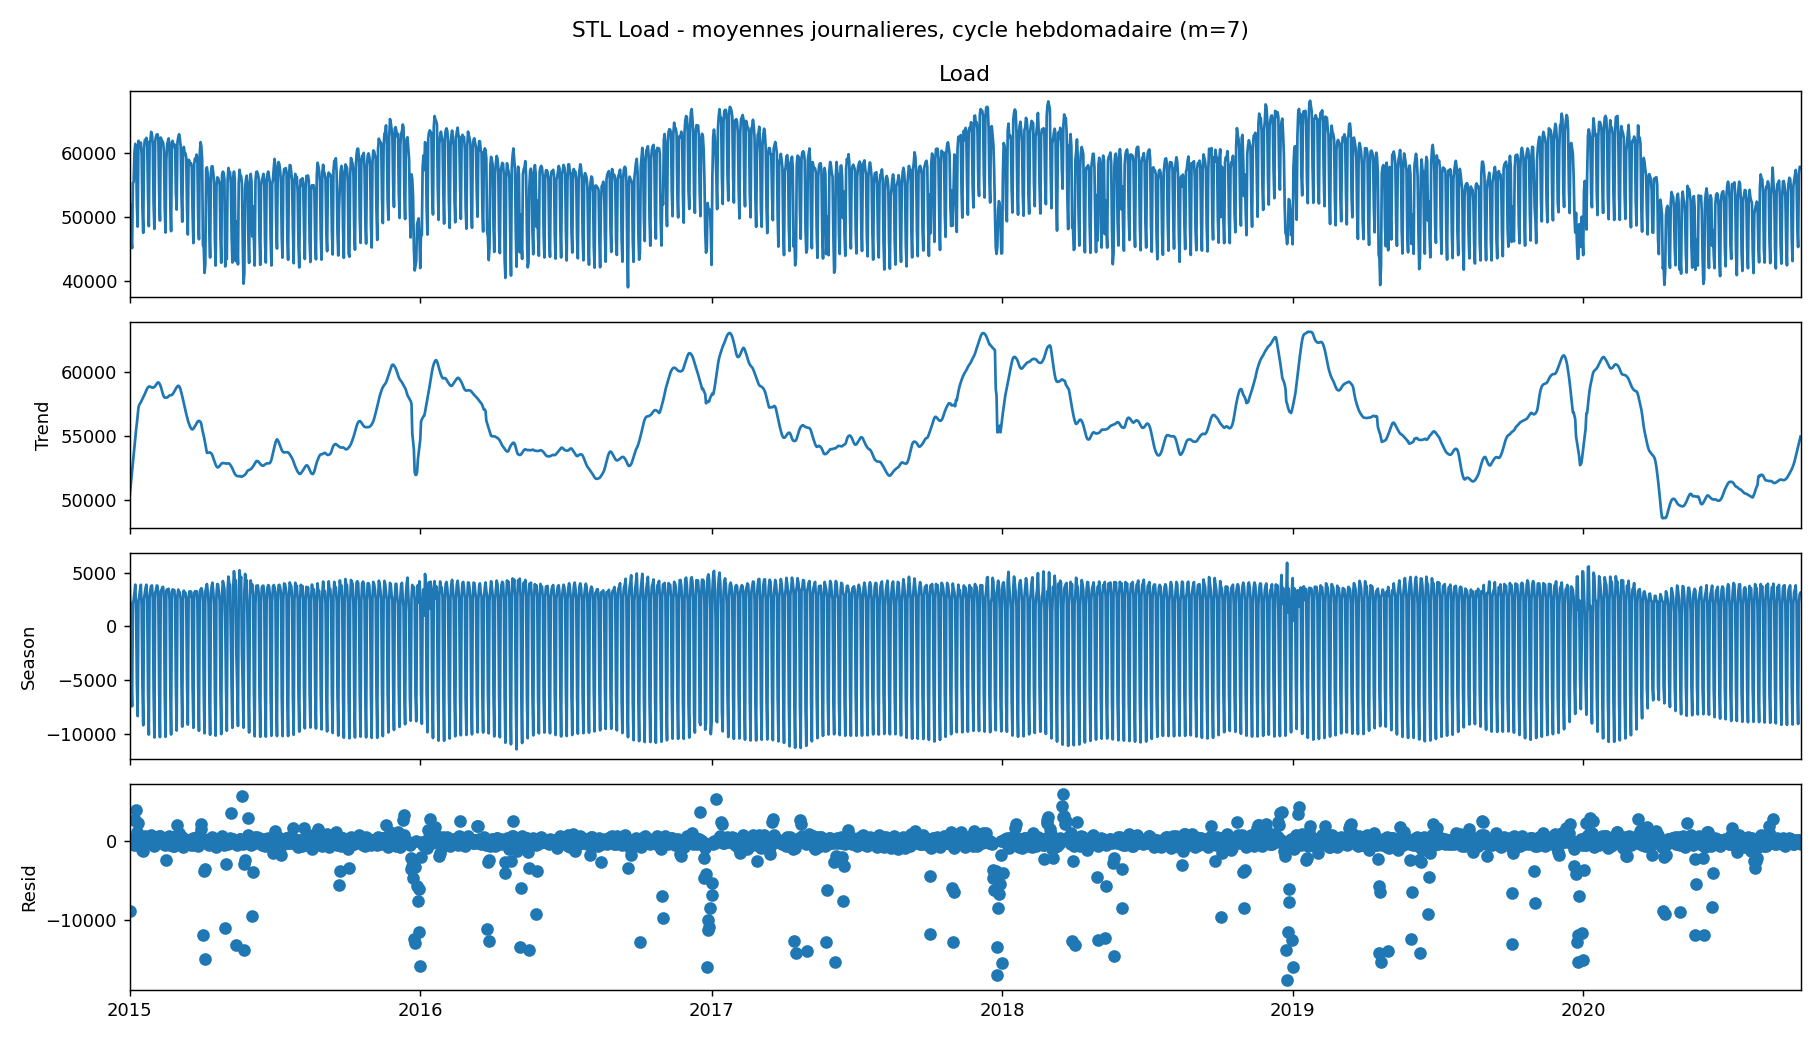
\includegraphics[width=0.75\textwidth]{py_stl_load_weekly.png}
\caption{Décomposition STL de la charge (cycle hebdomadaire).}
\label{fig:stl_weekly}
\end{figure}

\subsubsection{Valeurs manquantes et valeurs atypiques}
Les valeurs manquantes (figure~\ref{fig:missing_r} et~\ref{fig:missing_py})
sont rares et éparses. Le tableau~\ref{tab:outliers} montre que la règle IQR
globale ne détecte aucun point, tandis que la MAD roulante sur \(24\)~h
identifie \(761\) points atypiques (\(1{,}51\,\%\)) --- principalement des
épisodes éoliens extrêmes, illustrés par la figure~\ref{fig:outliers}.

\begin{figure}[H]
\centering
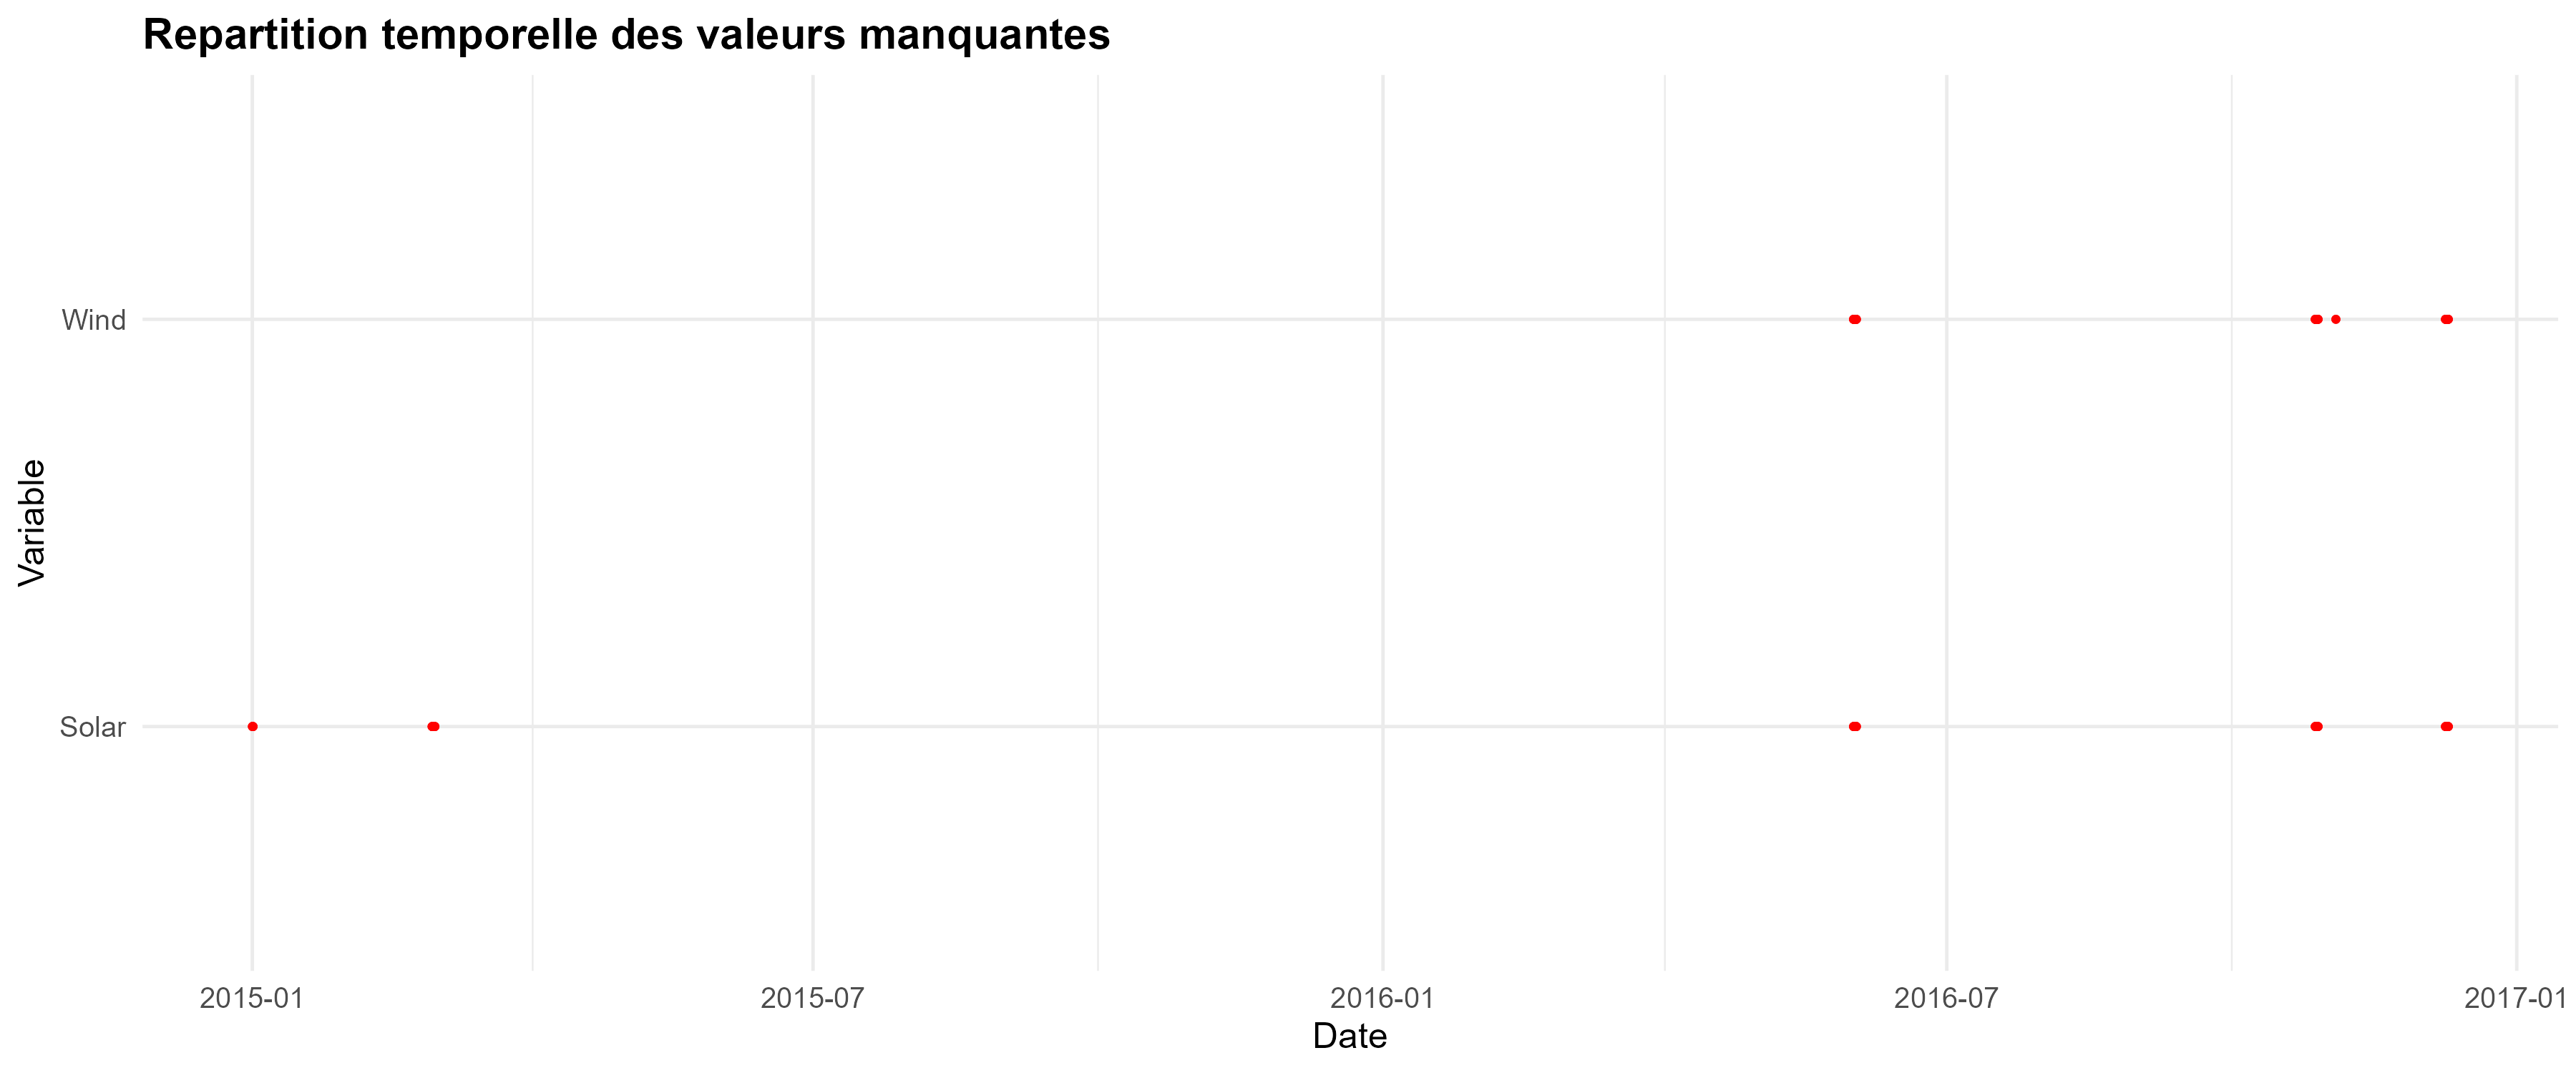
\includegraphics[width=0.9\textwidth]{missing_values.png}
\caption{Répartition temporelle des valeurs manquantes (R).}
\label{fig:missing_r}
\end{figure}

\begin{figure}[H]
\centering
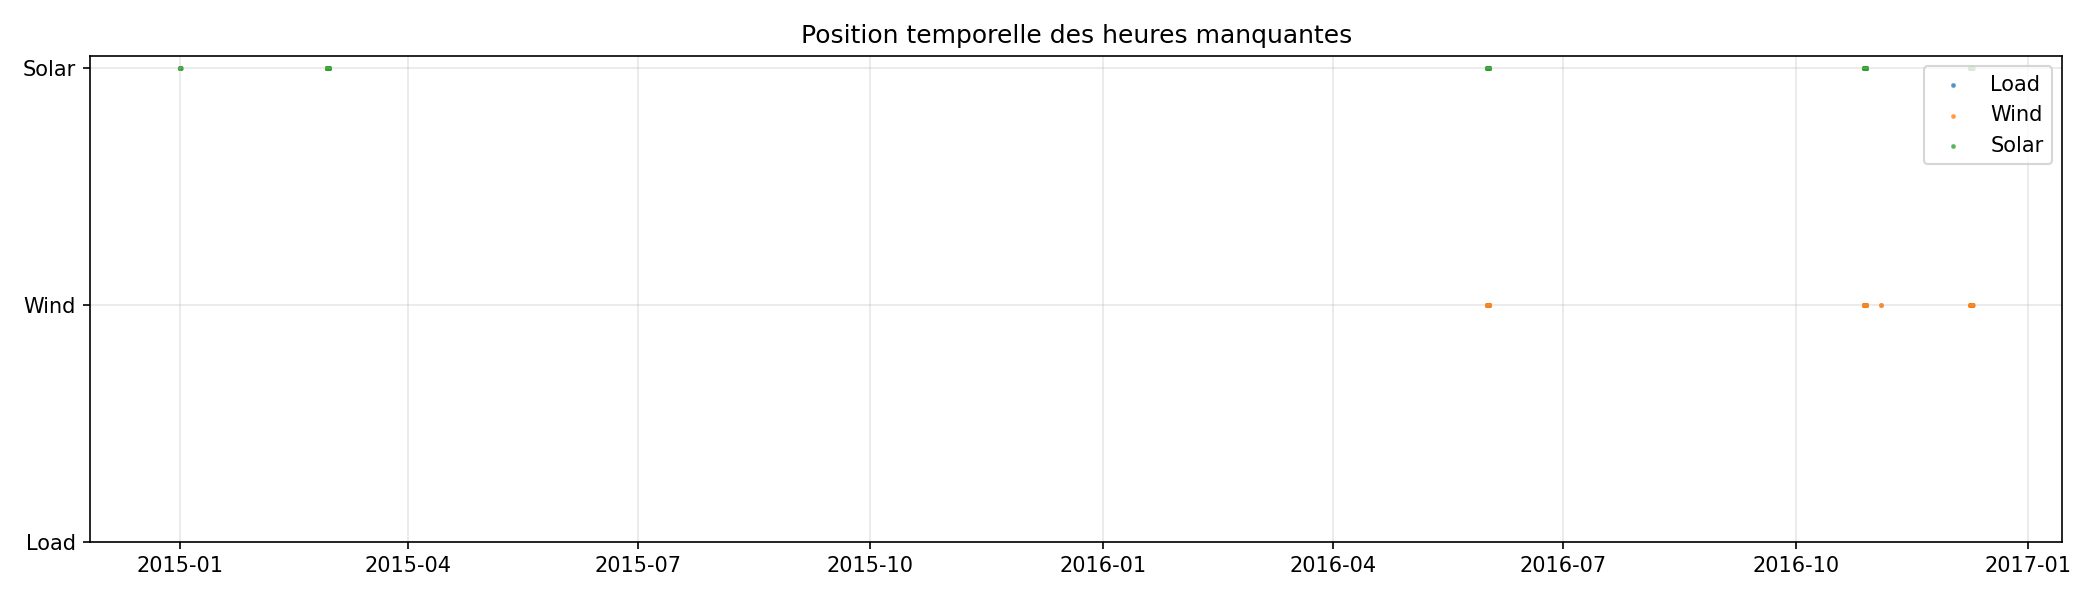
\includegraphics[width=0.9\textwidth]{py_missing.png}
\caption{Répartition temporelle des valeurs manquantes (Python).}
\label{fig:missing_py}
\end{figure}

\begin{table}[H]
\centering
\caption{Détection d'observations atypiques. Source : \texttt{outliers\_summary.csv}.}
\label{tab:outliers}
\begin{tabular}{lrr}
\toprule
Méthode & Nombre d'outliers & Part (\%) \\
\midrule
IQR global & 0 & 0{,}00 \\
MAD roulante 24~h & 761 & 1{,}51 \\
\bottomrule
\end{tabular}
\end{table}

\begin{figure}[H]
\centering
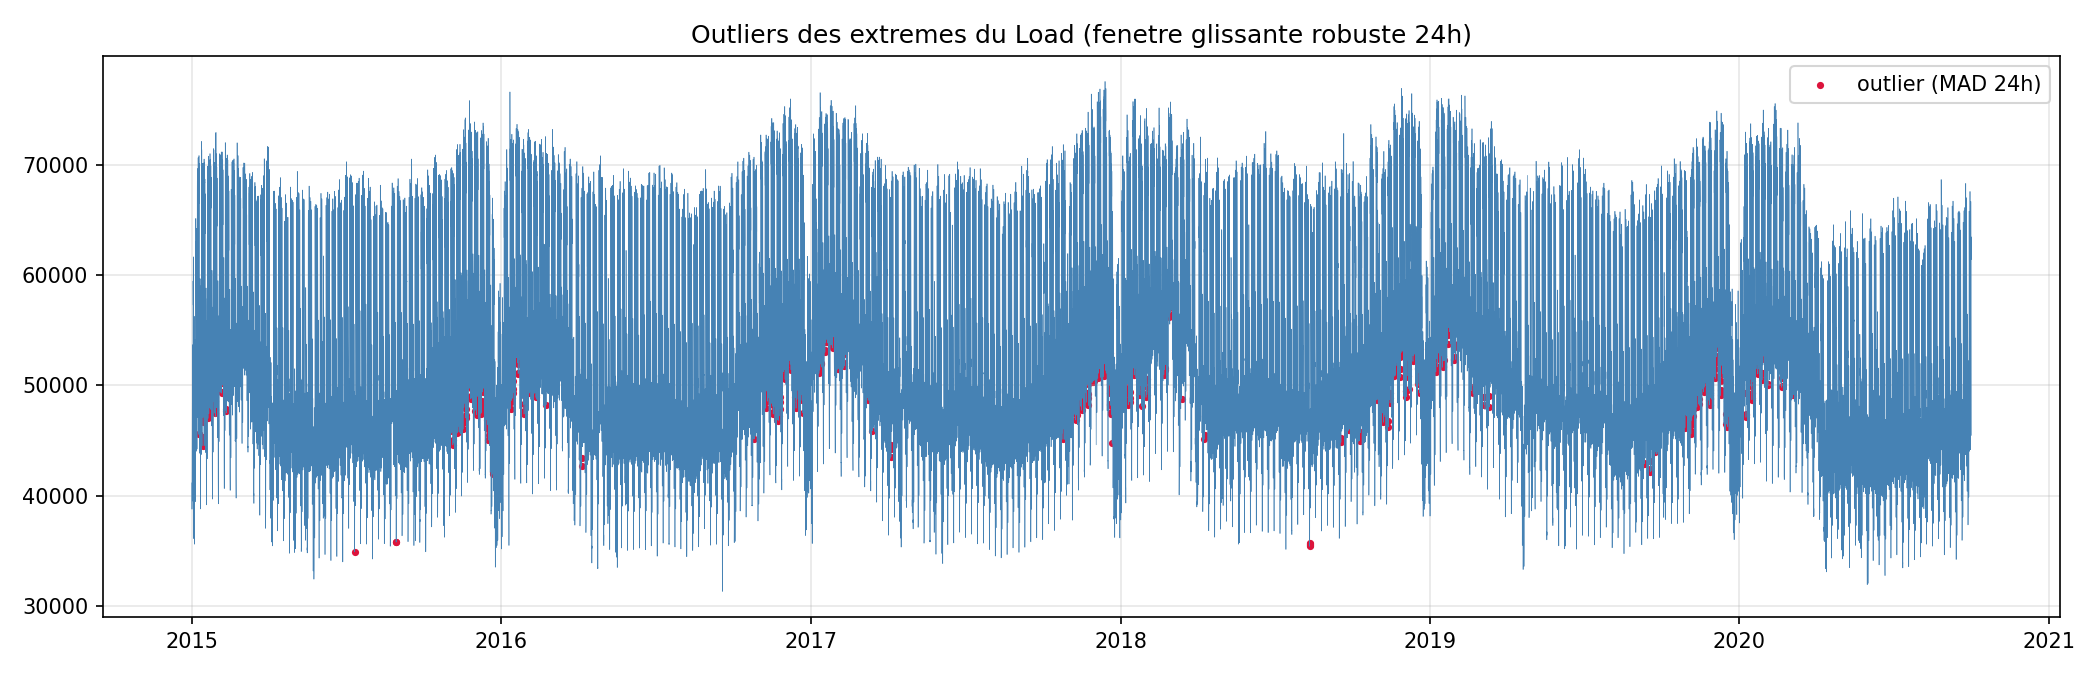
\includegraphics[width=0.85\textwidth]{py_outliers_load.png}
\caption{Détection d'outliers sur la charge (MAD roulante).}
\label{fig:outliers}
\end{figure}

\subsubsection{Stationnarité}
Le tableau~\ref{tab:stationnarite} (résultat R) montre que les séries brutes
sont jugées non stationnaires (ADF rejette la racine unitaire mais KPSS rejette
la stationnarité : les deux tests divergent). En différence première
(\(d=1\)), ADF et KPSS s'accordent : les séries sont \textbf{stationnaires}.
Ceci justifie l'usage de \(d=1\) dans les modèles ARIMA et de \(D1\) dans le
VAR/GARCH. Les conclusions sont identiques côté Python
(\texttt{stationarity\_tests.csv}).

\begin{table}[H]
\centering
\caption{Tests de stationnarité ADF / KPSS (R). Source : \texttt{R\_stationarity\_tests.csv}.}
\label{tab:stationnarite}
\small
\begin{tabular}{llrrrrl}
\toprule
Variable & Transf. & ADF stat & ADF p & KPSS stat & KPSS p & Stationnaire ? \\
\midrule
\texttt{Load}  & brute & $-24{,}75$ & 0{,}01 & 2{,}497 & 0{,}01 & Non \\
\texttt{Load}  & $d1$  & $-42{,}49$ & 0{,}01 & 0{,}0007 & 0{,}10 & Oui \\
\texttt{Wind}  & brute & $-18{,}68$ & 0{,}01 & 17{,}363 & 0{,}01 & Non \\
\texttt{Wind}  & $d1$  & $-44{,}68$ & 0{,}01 & 0{,}0005 & 0{,}10 & Oui \\
\texttt{Solar} & brute & $-11{,}69$ & 0{,}01 & 10{,}792 & 0{,}01 & Non \\
\texttt{Solar} & $d1$  & $-46{,}02$ & 0{,}01 & 0{,}0004 & 0{,}10 & Oui \\
\bottomrule
\end{tabular}
\end{table}

\subsubsection{Corrélogrammes ACF / PACF}
Les figures~\ref{fig:acf_load_raw} à~\ref{fig:acf_solar_d1} présentent les
ACF/PACF (R puis Python). Les séries brutes affichent une décroissance lente
et des rebonds marqués à \(24\) et \(168\) (saisonnalité quotidienne et
hebdomadaire). Après différenciation, les autocorrélations restent
significatives aux retards saisonniers, motivant la composante saisonnière
\((1,1,1)_{24}\).

\begin{figure}[H]
\centering
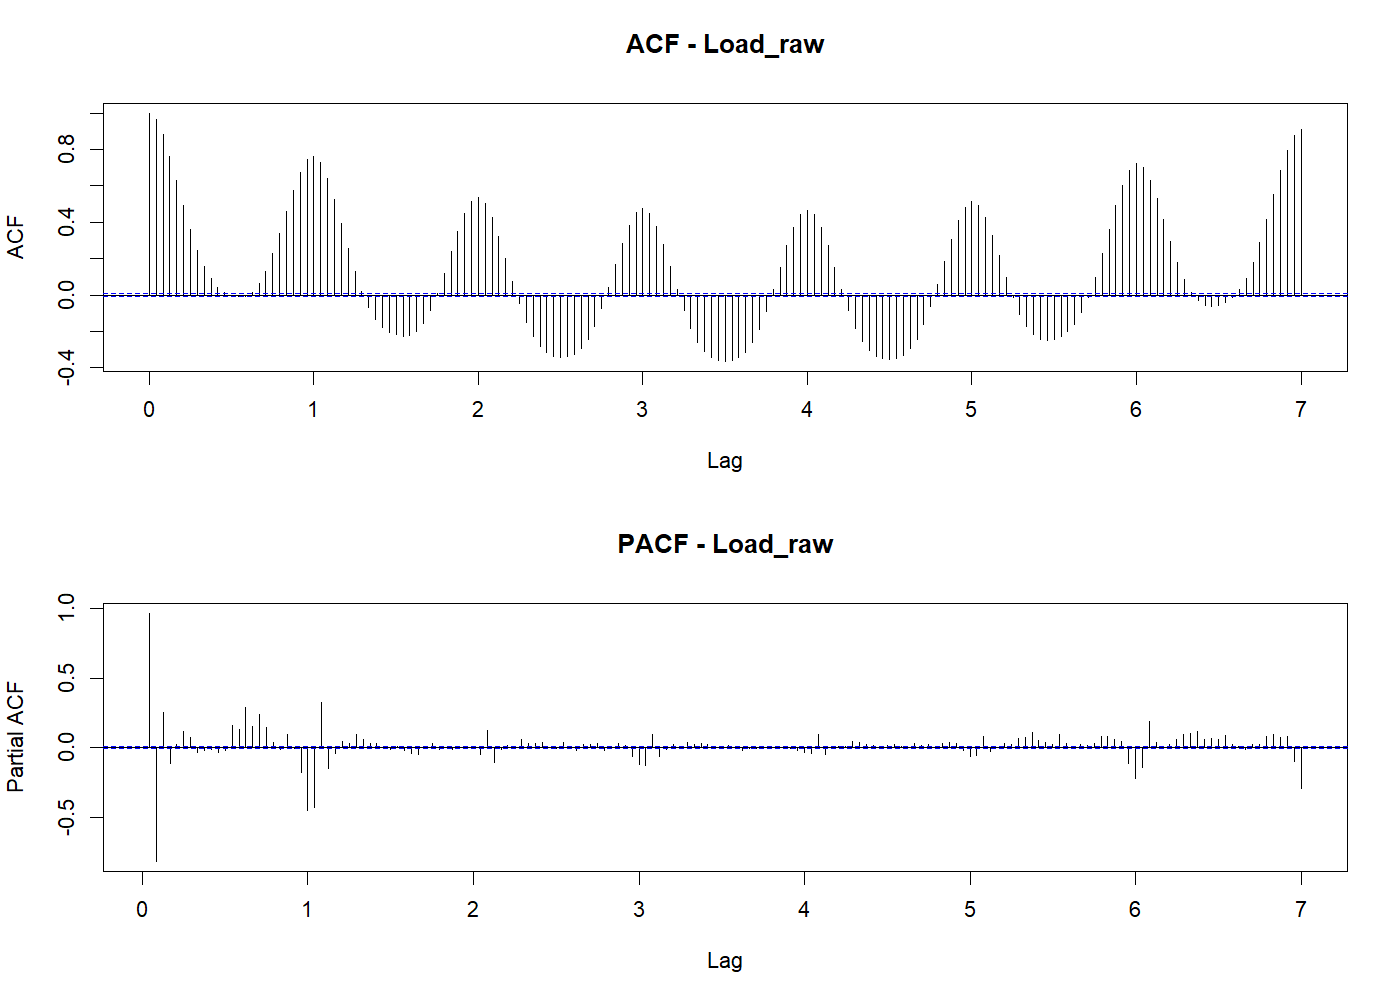
\includegraphics[width=0.95\textwidth]{R_acf_pacf_Load_raw.png}
\caption{ACF/PACF de \texttt{Load} (série brute, R).}
\label{fig:acf_load_raw}
\end{figure}

\begin{figure}[H]
\centering
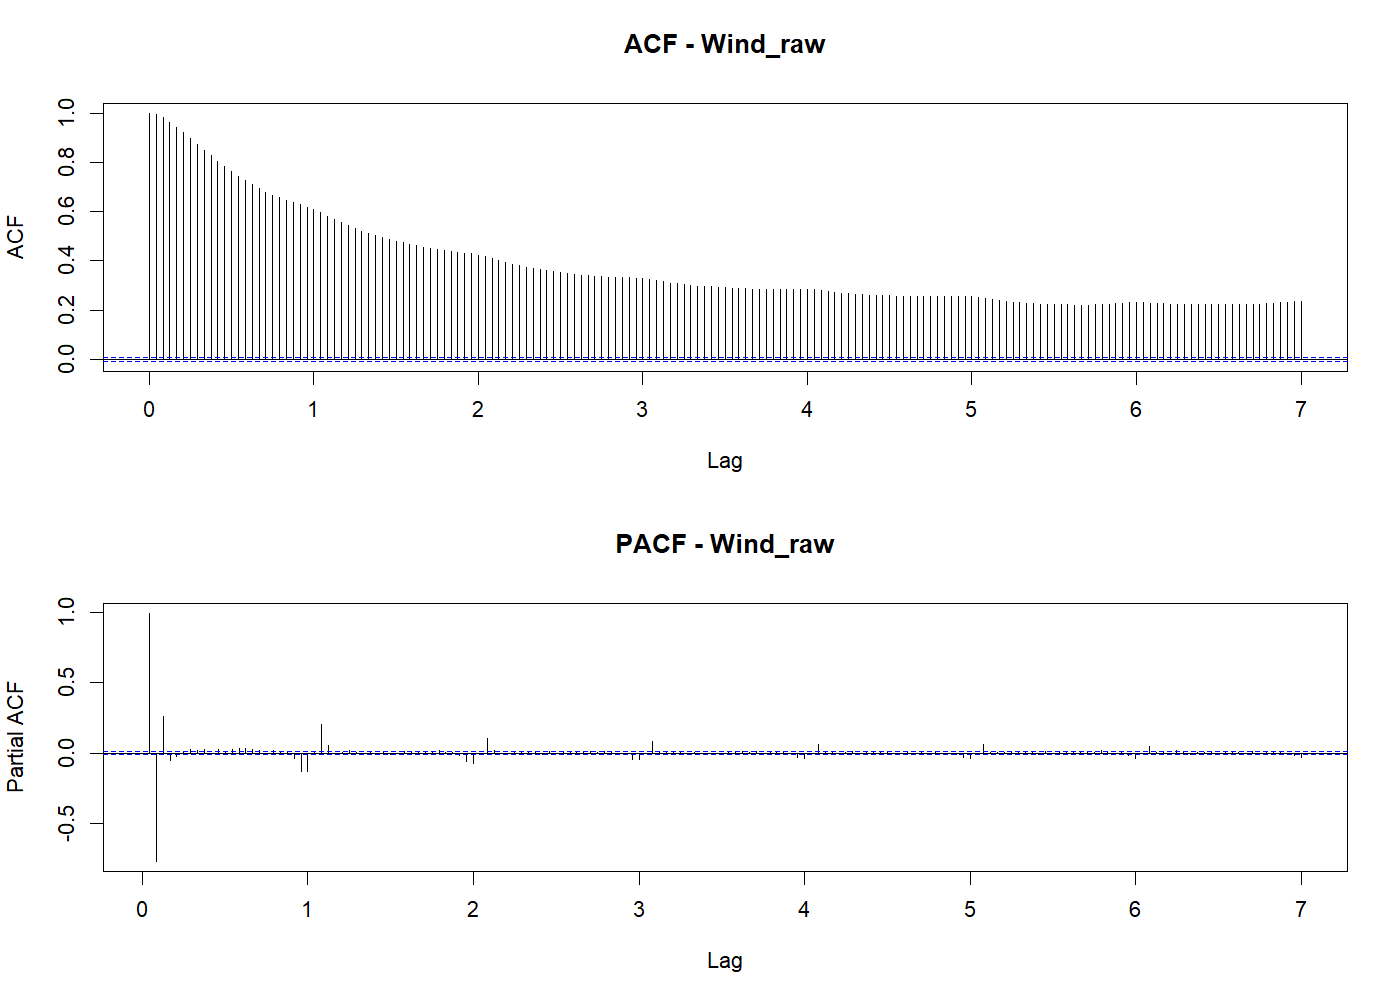
\includegraphics[width=0.95\textwidth]{R_acf_pacf_Wind_raw.png}
\caption{ACF/PACF de \texttt{Wind} (série brute, R).}
\label{fig:acf_wind_raw}
\end{figure}

\begin{figure}[H]
\centering
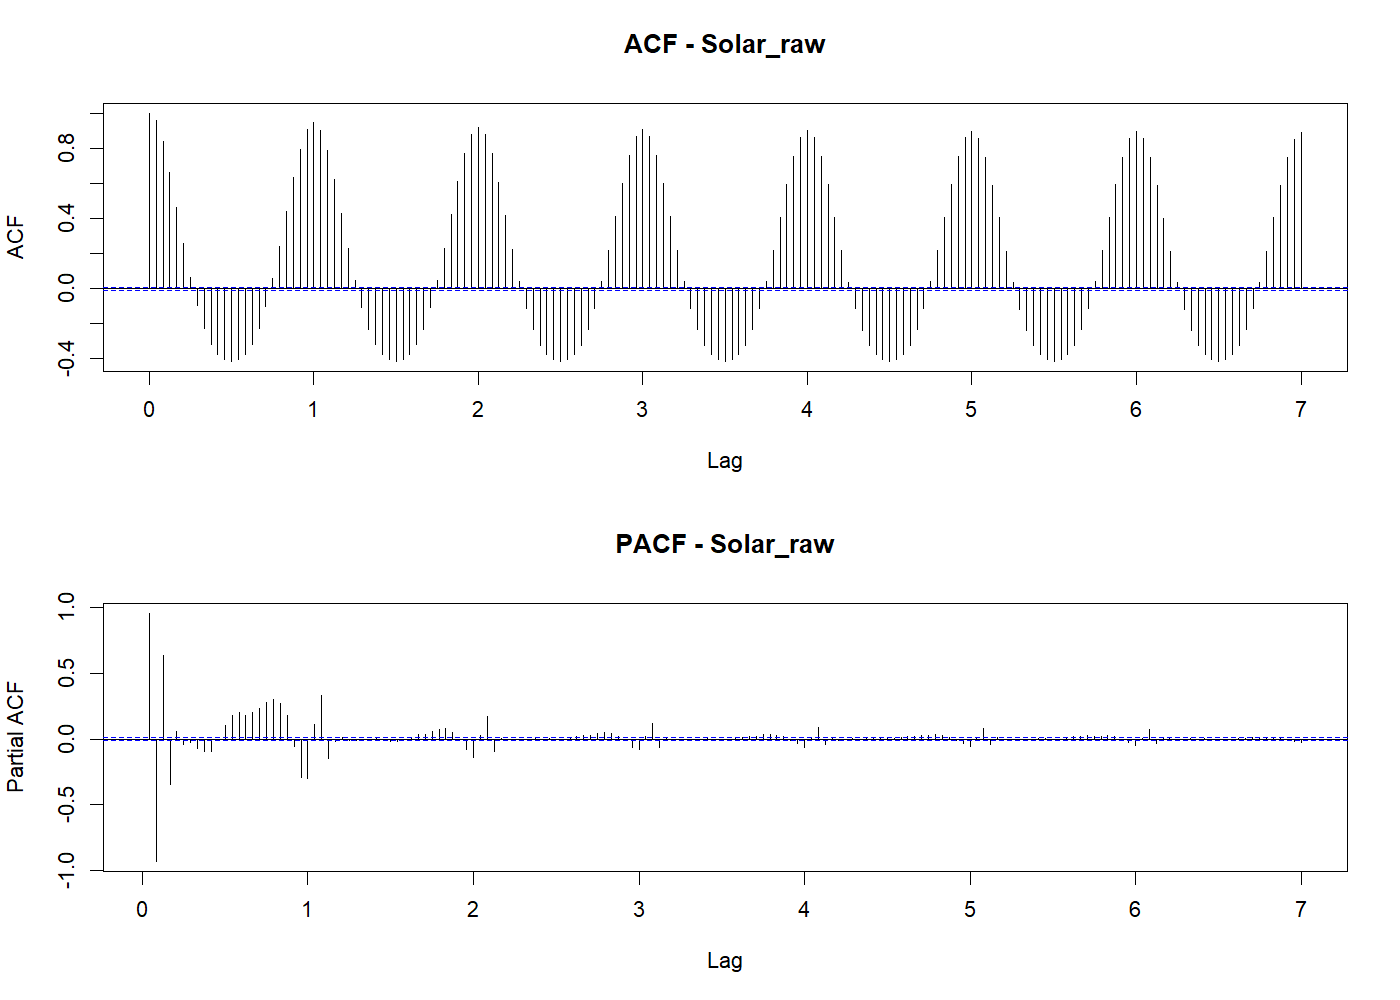
\includegraphics[width=0.95\textwidth]{R_acf_pacf_Solar_raw.png}
\caption{ACF/PACF de \texttt{Solar} (série brute, R).}
\label{fig:acf_solar_raw}
\end{figure}

\begin{figure}[H]
\centering
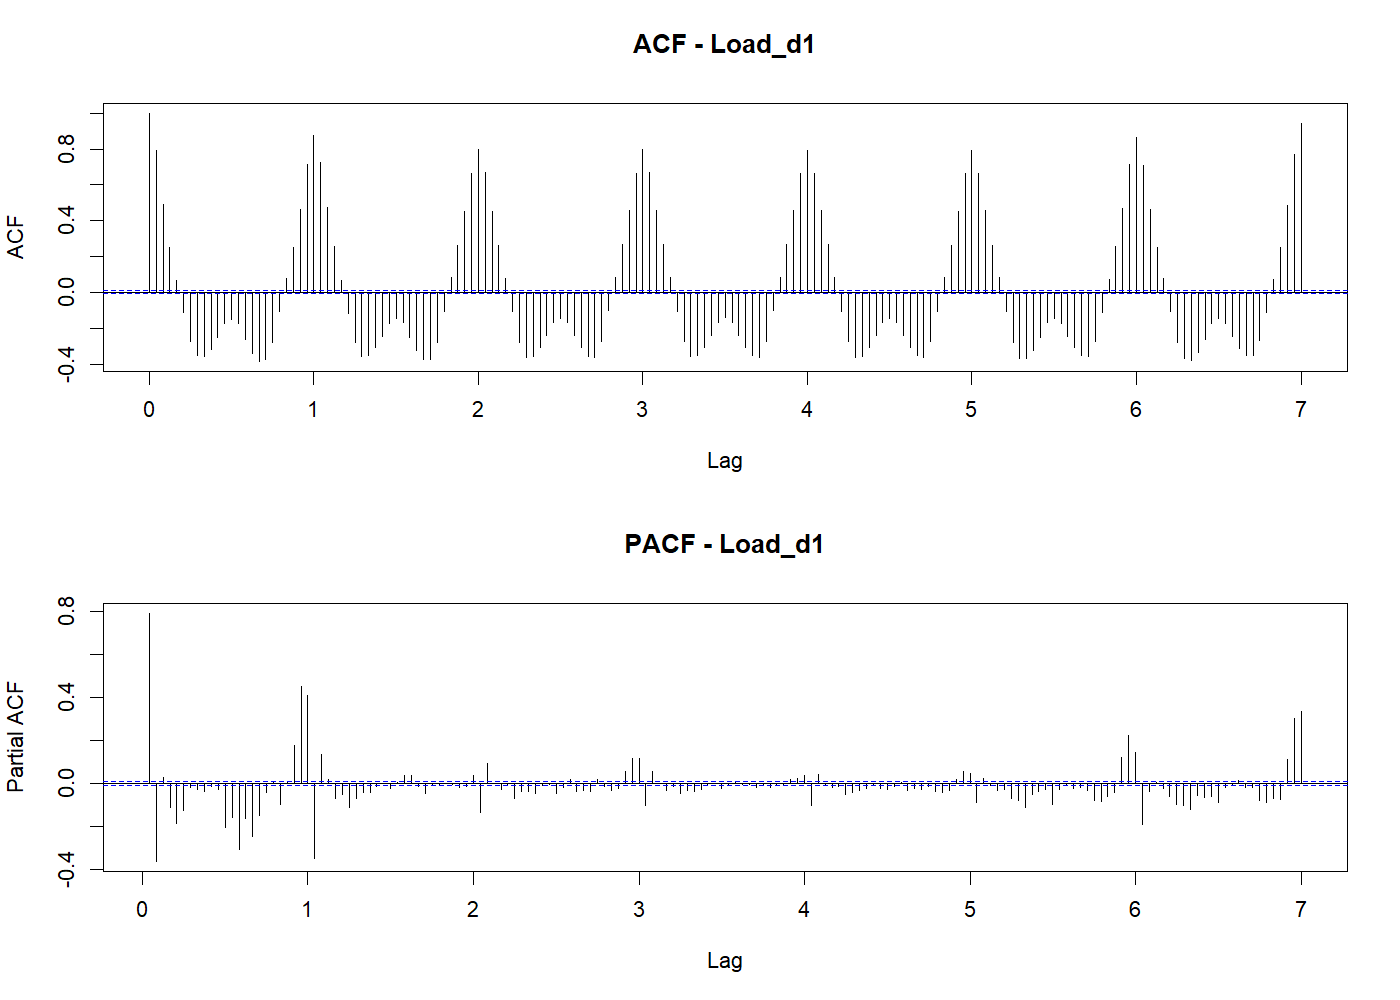
\includegraphics[width=0.95\textwidth]{R_acf_pacf_Load_d1.png}
\caption{ACF/PACF de \texttt{Load} différenciée ($d1$, R).}
\label{fig:acf_load_d1}
\end{figure}

\begin{figure}[H]
\centering
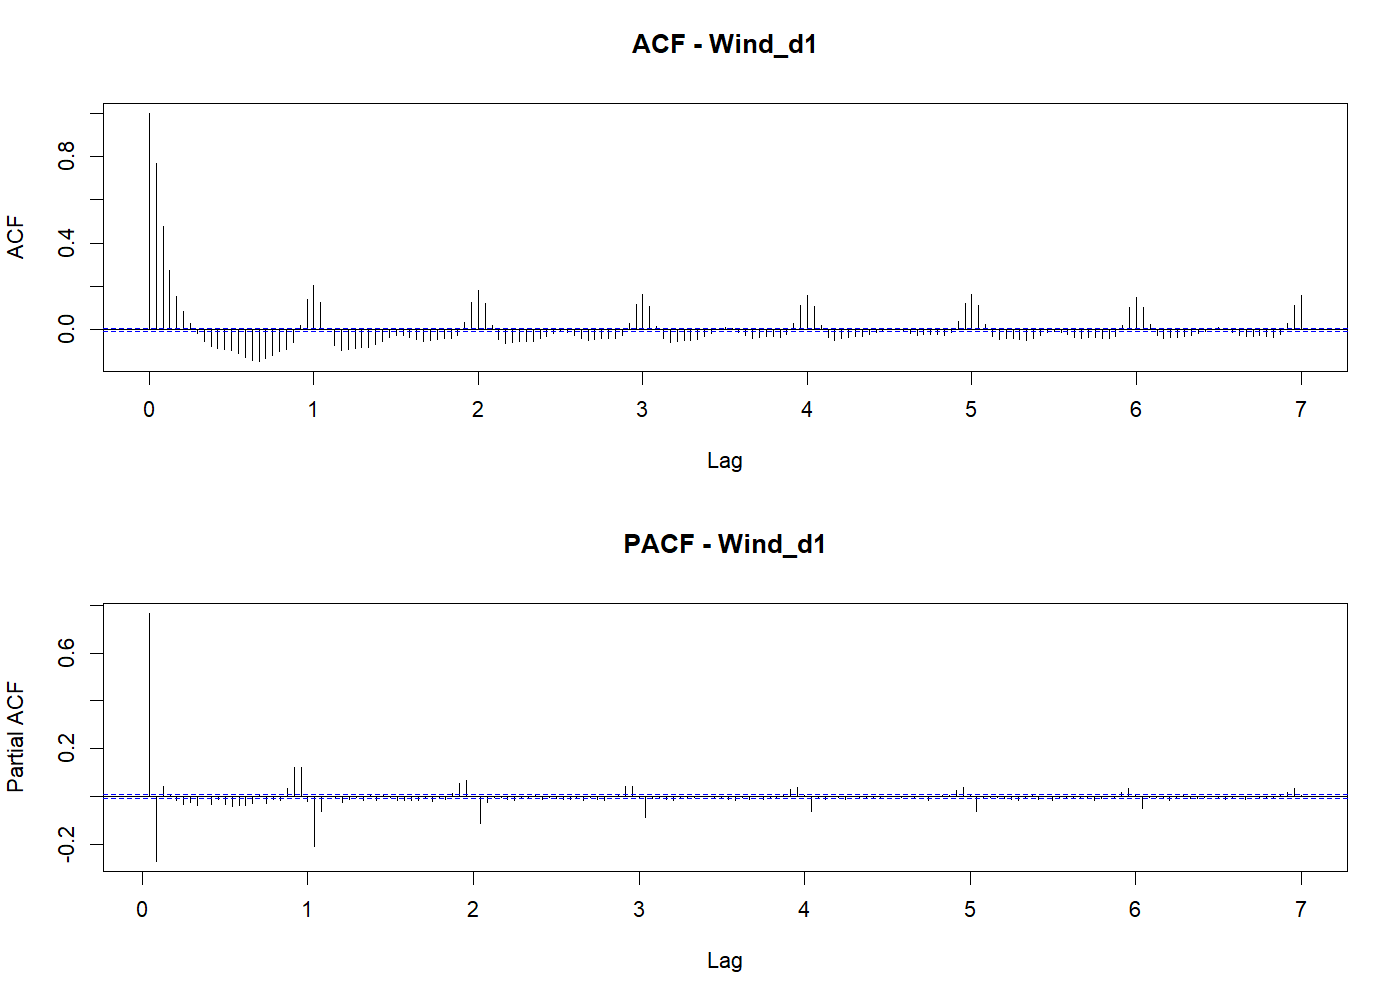
\includegraphics[width=0.95\textwidth]{R_acf_pacf_Wind_d1.png}
\caption{ACF/PACF de \texttt{Wind} différenciée ($d1$, R).}
\label{fig:acf_wind_d1}
\end{figure}

\begin{figure}[H]
\centering
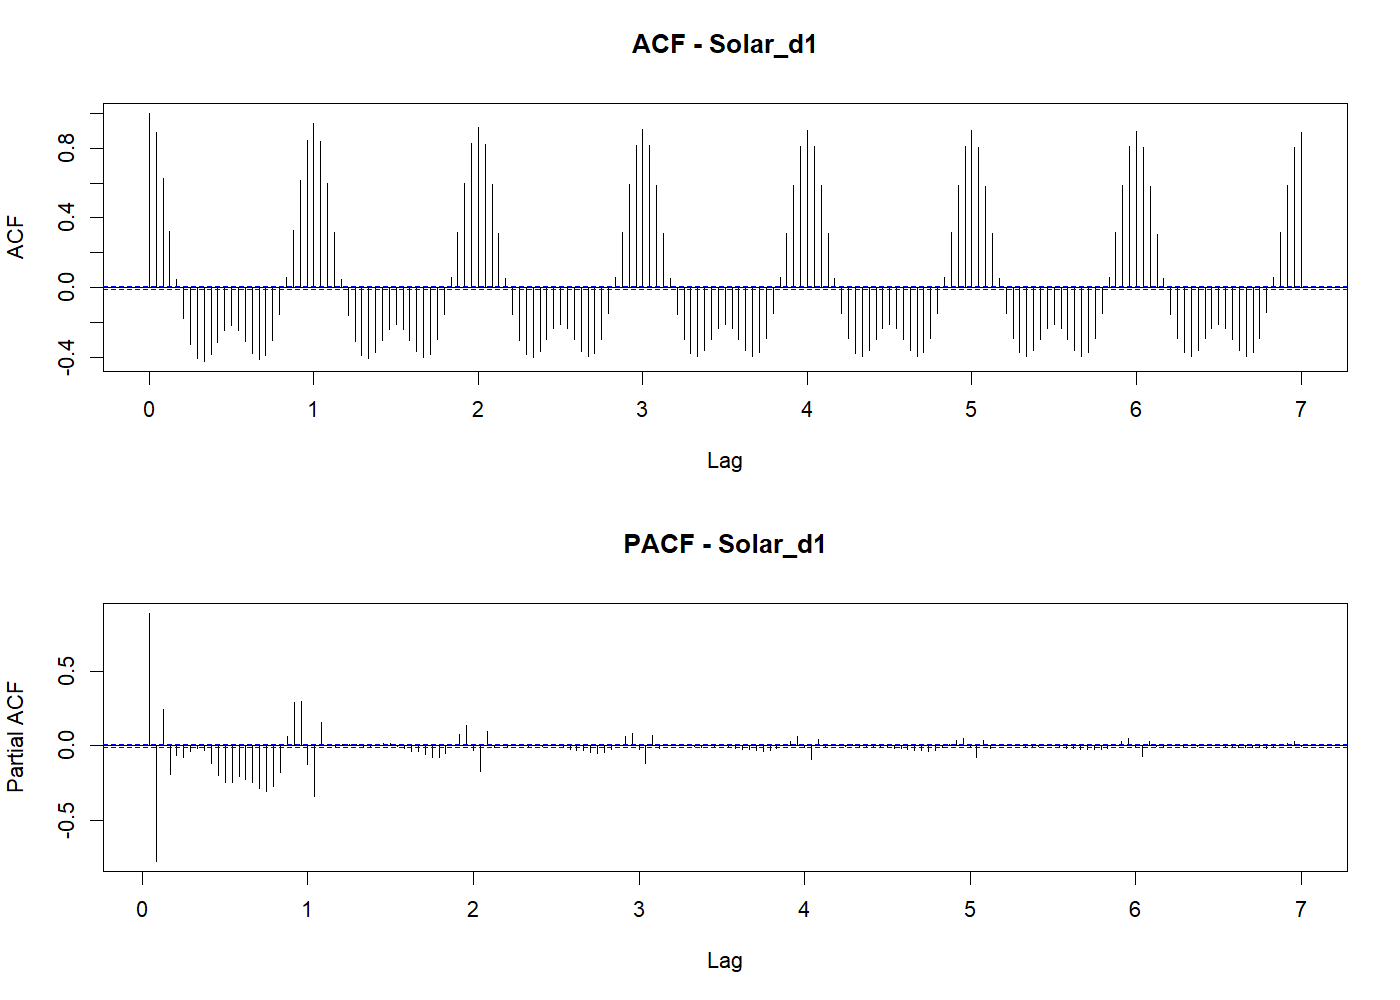
\includegraphics[width=0.95\textwidth]{R_acf_pacf_Solar_d1.png}
\caption{ACF/PACF de \texttt{Solar} différenciée ($d1$, R).}
\label{fig:acf_solar_d1}
\end{figure}

\begin{figure}[H]
\centering
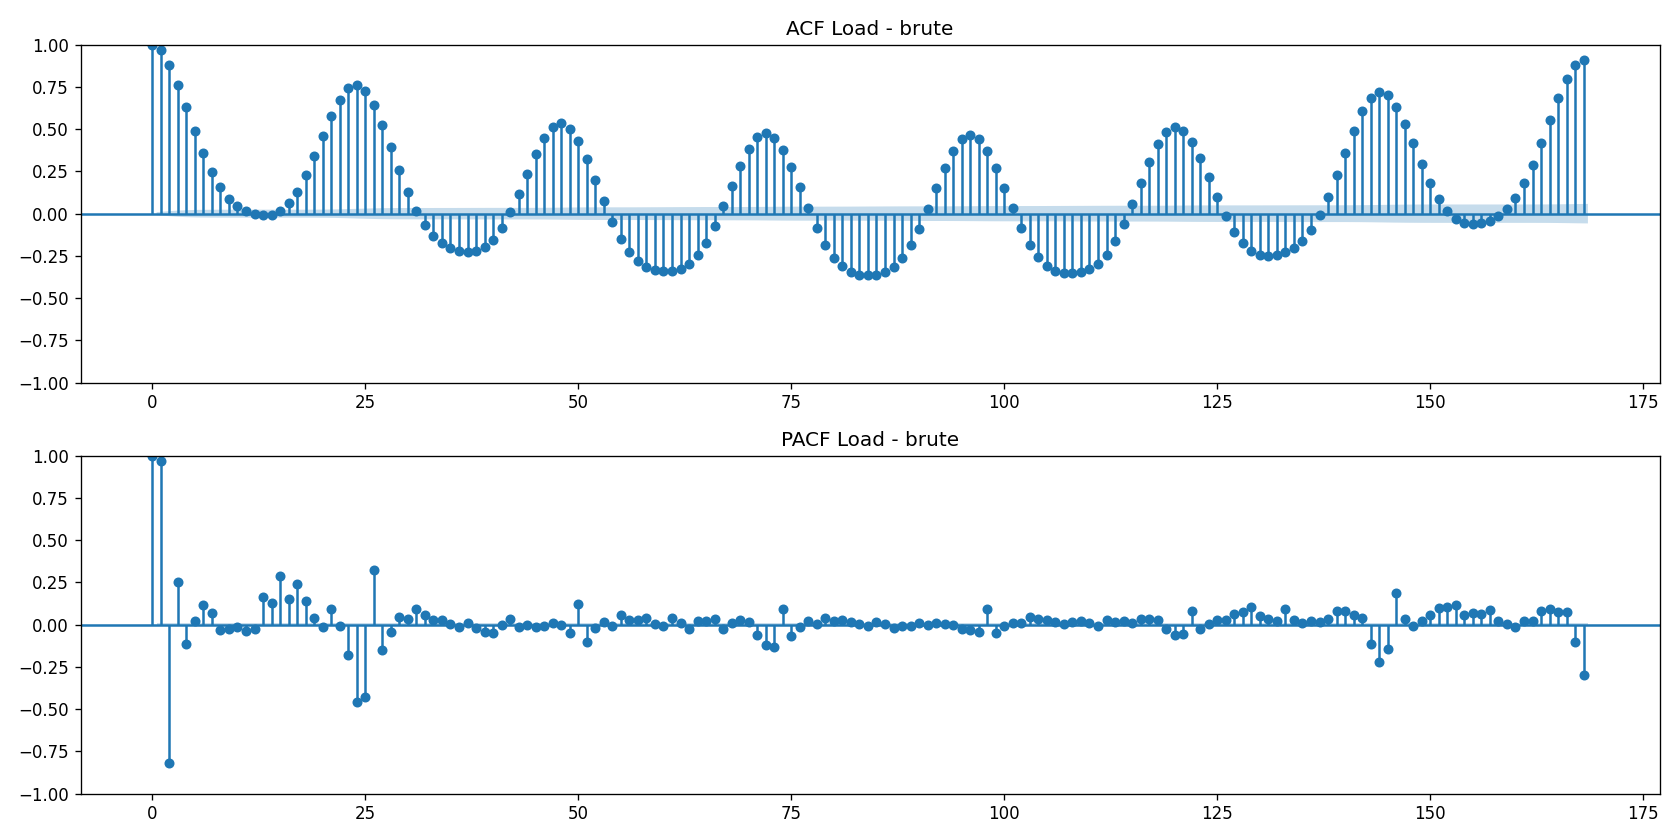
\includegraphics[width=0.8\textwidth]{py_acf_pacf_Load_raw.png}
\caption{ACF/PACF de \texttt{Load} brute (Python). À comparer avec la
figure~\ref{fig:acf_load_raw}.}
\label{fig:acf_py_load}
\end{figure}

\begin{figure}[H]
\centering
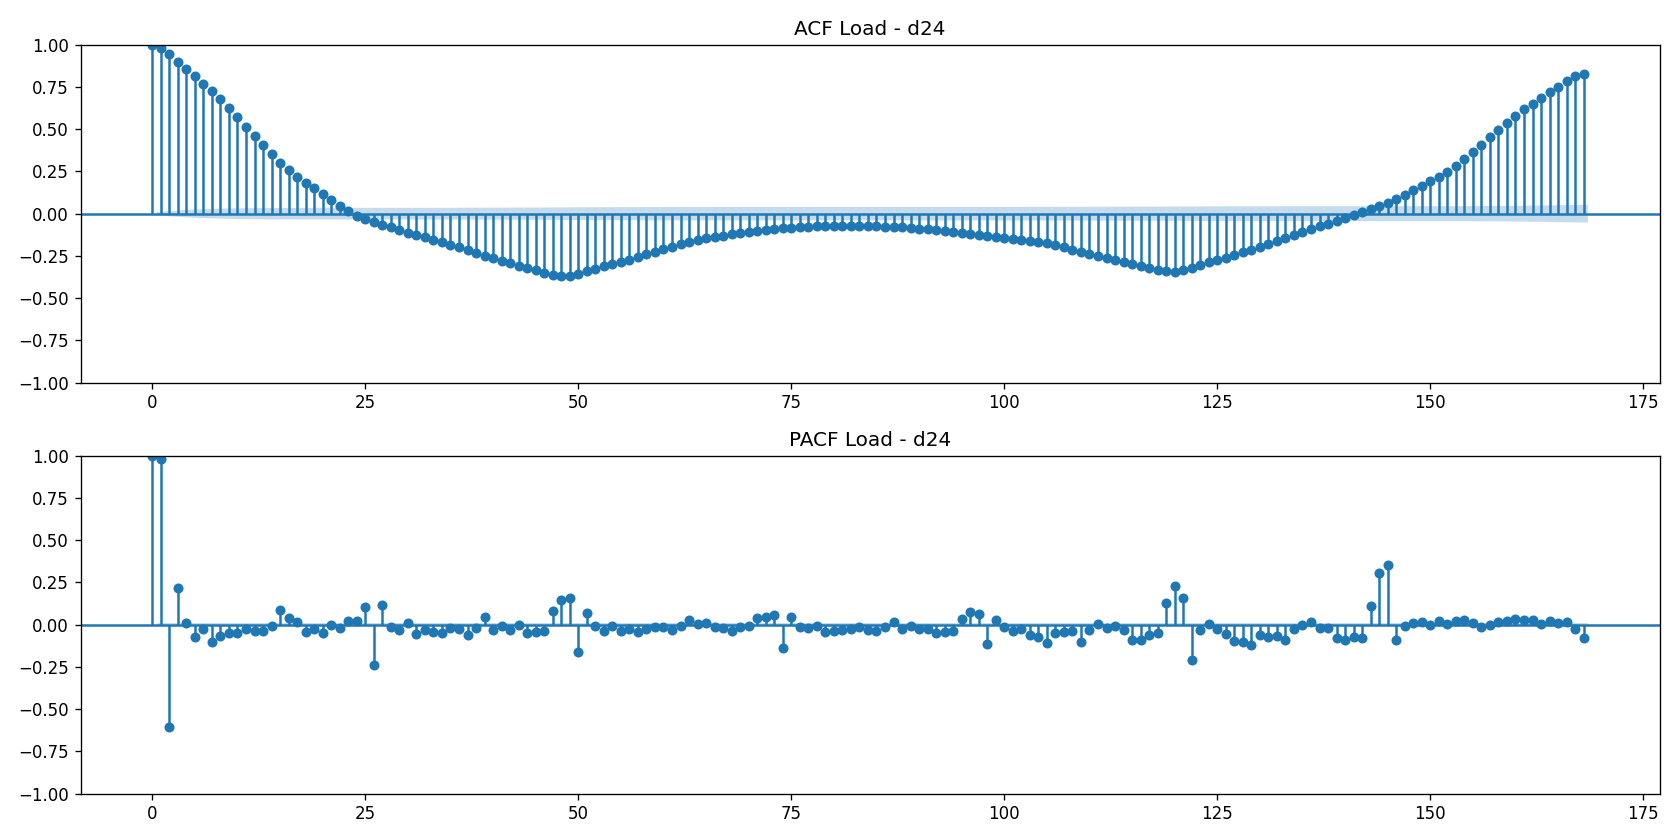
\includegraphics[width=0.95\textwidth]{py_acf_pacf_Load_d24.png}
\caption{ACF/PACF de \texttt{Load} en différence saisonnière ($d24$, Python).}
\label{fig:acf_py_load_d24}
\end{figure}

\begin{figure}[H]
\centering
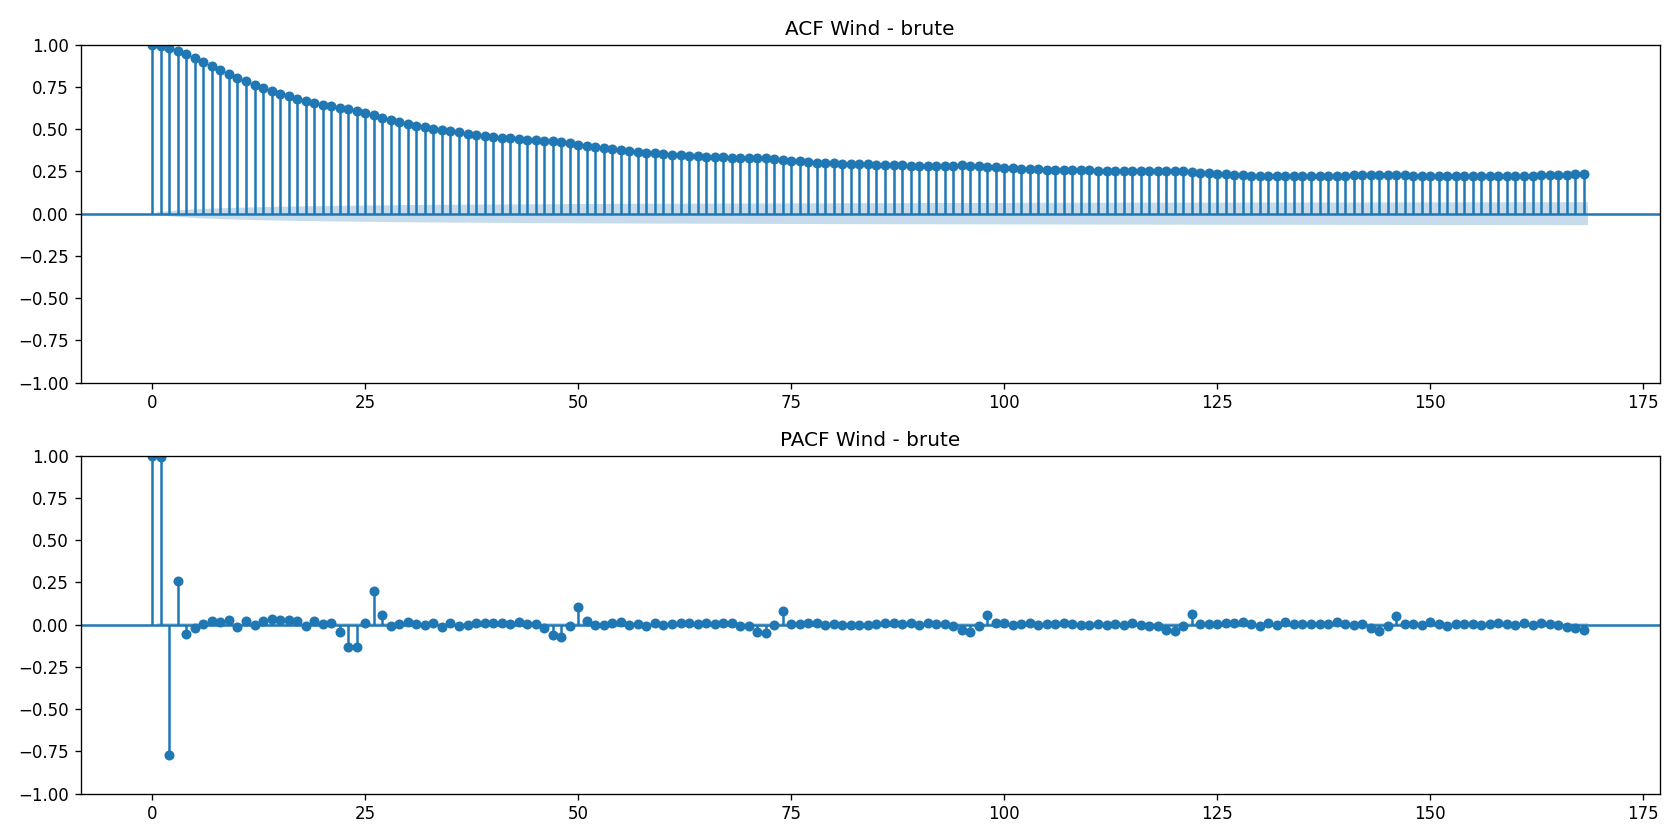
\includegraphics[width=0.95\textwidth]{py_acf_pacf_Wind_raw.png}
\caption{ACF/PACF de \texttt{Wind} brute (Python).}
\label{fig:acf_py_wind}
\end{figure}

\begin{figure}[H]
\centering
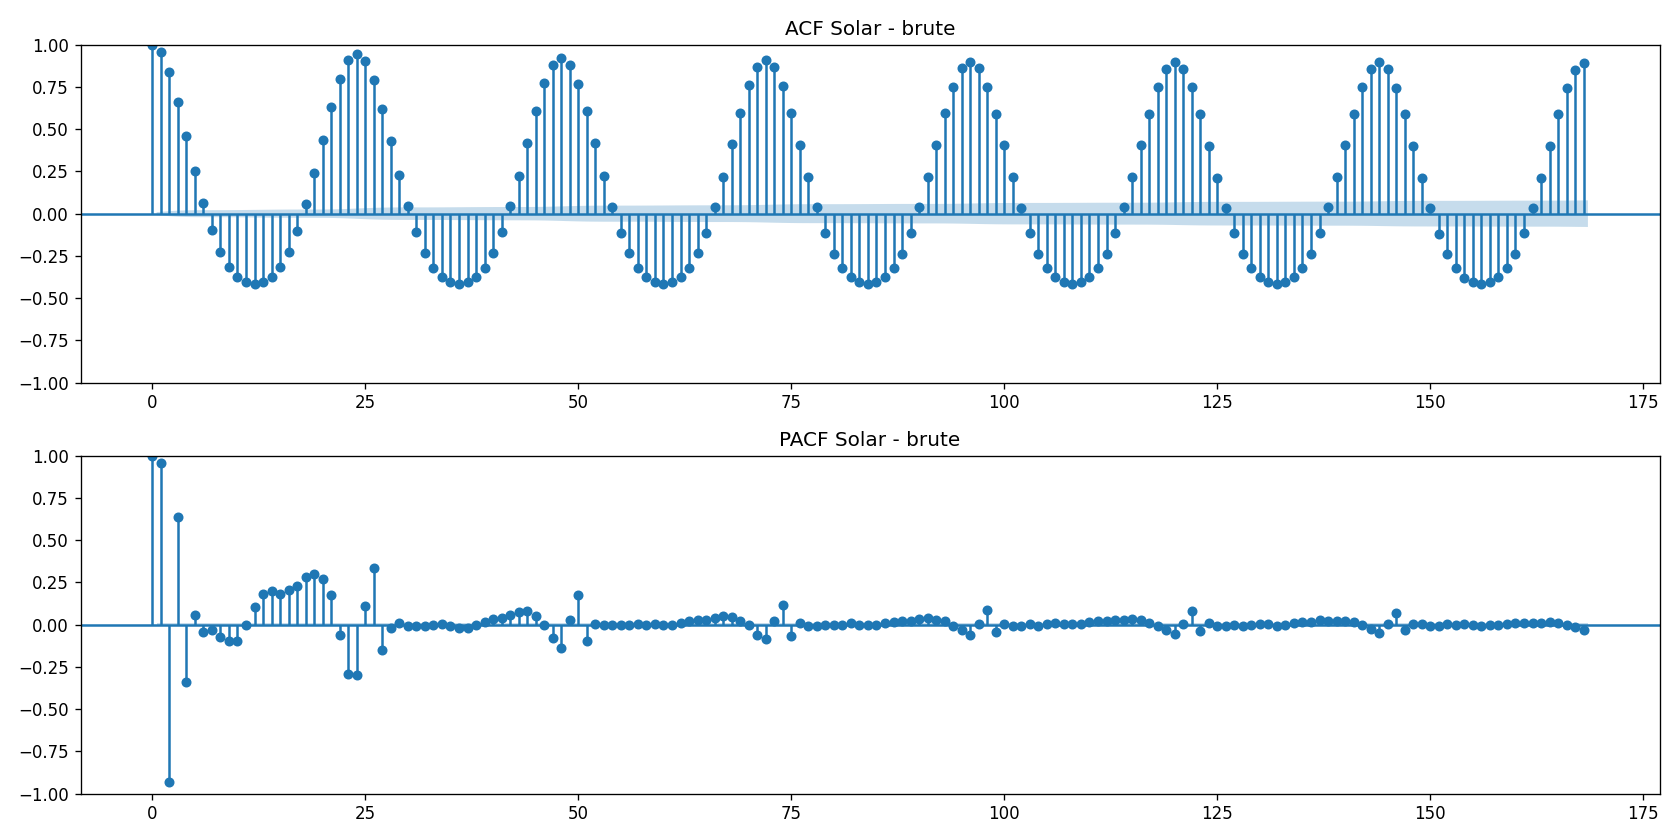
\includegraphics[width=0.95\textwidth]{py_acf_pacf_Solar_raw.png}
\caption{ACF/PACF de \texttt{Solar} brute (Python).}
\label{fig:acf_py_solar}
\end{figure}

\FloatBarrier

\subsection{Socle univarié : ARIMA / SARIMA}

\subsubsection{Sélection des modèles}
Le tableau~\ref{tab:arima_comp_r} (R) et le tableau~\ref{tab:arima_comp_py}
(Python) comparent les trois candidats par AIC/AICc/BIC. Les deux
implémentations retiennent des ordres \textbf{identiques} :
\begin{itemize}
  \item \texttt{Load} : \texttt{SARIMA\_manuel} \(\text{ARIMA}(1,1,1)(1,1,1)_{24}\)
        (AICc minimal) ;
  \item \texttt{Wind} : \texttt{SARIMA\_manuel} également retenu ;
  \item \texttt{Solar} : \texttt{SARIMA\_auto} \(\text{ARIMA}(2,1,2)(0,1,1)_{24}\)
        au plus faible AICc.
\end{itemize}
Le modèle non saisonnier \texttt{ARIMA\_auto} présente systématiquement un
AICc nettement supérieur, confirmant la nécessité de la composante saisonnière
\(m=24\).

\begin{table}[H]
\centering
\caption{Comparaison des modèles ARIMA/SARIMA (R). AICc minimal en gras.
Source : \texttt{R\_arima\_model\_comparison.csv}.}
\label{tab:arima_comp_r}
\small
\begin{tabular}{llrrrl}
\toprule
Variable & Modèle & AIC & AICc & BIC & Spécification \\
\midrule
\texttt{Load}  & SARIMA\_manuel & 740\,406 & \textbf{740\,406{,}22} & 740\,450 & ARIMA(1,1,1)(1,1,1)[24] \\
\texttt{Load}  & ARIMA\_auto    & 786\,041 & 786\,041{,}00 & 786\,102 & ARIMA(5,1,1) \\
\texttt{Load}  & SARIMA\_auto   & 752\,342 & 752\,341{,}81 & 752\,394 & ARIMA(2,1,2)(1,1,0)[24] \\
\texttt{Wind}  & SARIMA\_manuel & 694\,884 & \textbf{694\,884{,}46} & 694\,928 & ARIMA(1,1,1)(1,1,1)[24] \\
\texttt{Wind}  & ARIMA\_auto    & 701\,054 & 701\,054{,}37 & 701\,115 & ARIMA(2,1,3) \\
\texttt{Wind}  & SARIMA\_auto   & 698\,594 & 698\,594{,}09 & 698\,638 & ARIMA(1,1,2)(1,0,0)[24] \\
\texttt{Solar} & SARIMA\_manuel & 656\,144 & 656\,143{,}85 & 656\,187 & ARIMA(1,1,1)(1,1,1)[24] \\
\texttt{Solar} & ARIMA\_auto    & 700\,943 & 700\,943{,}17 & 700\,987 & ARIMA(2,1,2) \\
\texttt{Solar} & SARIMA\_auto   & 650\,435 & \textbf{650\,434{,}88} & 650\,487 & ARIMA(2,1,2)(0,1,1)[24] \\
\bottomrule
\end{tabular}
\end{table}

\begin{table}[H]
\centering
\caption{Comparaison des modèles ARIMA/SARIMA (Python) --- confirme les ordres
retenus en R. Source : \texttt{py\_arima\_model\_comparison.csv}.}
\label{tab:arima_comp_py}
\small
\begin{tabular}{llrrrl}
\toprule
Variable & Modèle & AIC & AICc & BIC & Spécification \\
\midrule
\texttt{Load}  & SARIMA\_manuel & 739\,990 & 739\,990 & 740\,033 & ARIMA(1,1,1)(1,1,1)[24] \\
\texttt{Load}  & ARIMA\_auto    & 786\,510 & 786\,510 & 786\,571 & ARIMA(5,1,1) \\
\texttt{Load}  & SARIMA\_auto   & 752\,042 & 752\,042 & 752\,095 & ARIMA(2,1,2)(1,1,0)[24] \\
\texttt{Wind}  & ARIMA\_auto    & 701\,099 & 701\,099 & 701\,152 & ARIMA(2,1,3) \\
\texttt{Wind}  & SARIMA\_auto   & 698\,280 & 698\,280 & 698\,324 & ARIMA(1,1,2)(1,0,0)[24] \\
\texttt{Solar} & SARIMA\_manuel & 655\,665 & 655\,665 & 655\,709 & ARIMA(1,1,1)(1,1,1)[24] \\
\texttt{Solar} & ARIMA\_auto    & 701\,059 & 701\,059 & 701\,103 & ARIMA(2,1,2) \\
\texttt{Solar} & SARIMA\_auto   & 649\,997 & 649\,997 & 650\,049 & ARIMA(2,1,2)(0,1,1)[24] \\
\bottomrule
\end{tabular}
\end{table}

\subsubsection{Diagnostics des résidus}
Le tableau~\ref{tab:arima_diag} présente les diagnostics du meilleur modèle
par série. Quelle que soit l'implémentation, les trois tests rejettent leurs
hypothèses nulles : autocorrélation résiduelle partielle (Ljung--Box),
non-normalité (Jarque--Bera) et surtout \textbf{effet ARCH persistant}
(ARCH--LM), ce dernier point justifiant directement le volet GARCH
(section~\ref{sec:garch}).

\begin{table}[H]
\centering
\caption{Diagnostics des résidus du meilleur modèle ARIMA/SARIMA.
Sources : \texttt{R\_arima\_diagnostics.csv} et \texttt{py\_arima\_diagnostics.csv}.}
\label{tab:arima_diag}
\small
\begin{tabular}{llrrrr}
\toprule
Impl. & Variable & Ljung--Box(24) p & Jarque--Bera p & ARCH--LM(12) p & Verdict \\
\midrule
R  & \texttt{Load}  & $<0{,}001$ & $<0{,}001$ & $<0{,}001$ & Rejets \\
R  & \texttt{Wind}  & $<0{,}001$ & $<0{,}001$ & $<0{,}001$ & Rejets \\
R  & \texttt{Solar} & $<0{,}001$ & $<0{,}001$ & $<0{,}001$ & Rejets \\
py & \texttt{Load}  & $0{,}000$ & $0{,}000$ & $7{,}2\text{e-}240$ & Rejets \\
py & \texttt{Wind}  & $1{,}6\text{e-}65$ & $0{,}000$ & $0{,}000$ & Rejets \\
py & \texttt{Solar} & $6{,}2\text{e-}262$ & $0{,}000$ & $0{,}000$ & Rejets \\
\bottomrule
\end{tabular}
\end{table}

\subsubsection{Prévisions et métriques}
Le tableau~\ref{tab:arima_metrics} donne l'intégralité des métriques R.
Plusieurs enseignements se dégagent :
\begin{itemize}
  \item À \(h=10\) et \(h=24\), les RMSE sont faibles pour \texttt{Load}
        (SARIMA\_manuel : \(\approx 899\) puis \(1\,069\)~MW, soit
        \(\text{MAPE}\approx 1{,}4\,\%\)) et pour \texttt{Solar}
        (\texttt{SARIMA\_auto} : RMSE \(\approx 553\)~MW à \(h=10\)) ;
  \item À \(h=5\,040\), en revanche, les erreurs explosent (RMSE de
        \(65\,847\)~MW pour \texttt{Load} SARIMA\_manuel) : la prévision
        récursive sur \(7\) mois n'a plus de sens statistique, résultat
        documenté honnêtement ;
  \item le MAPE de \texttt{Solar} devient extrêmement élevé au voisinage des
        zéros (\(23\,953\,\%\) à \(h=5\,040\)), artefact bien connu de cette
        métrique lorsque le dénominateur s'annule.
\end{itemize}
Les prévisions (figures~\ref{fig:prev_r_load}--\ref{fig:prev_r_solar} et
Python~\ref{fig:prev_py_load}--\ref{fig:prev_py_solar}) et les graphiques de
diagnostic des résidus (figures~\ref{fig:resid_r_load}--\ref{fig:resid_r_solar}
et~\ref{fig:resid_py_load}--\ref{fig:resid_py_solar}) confirment ces
constats.

{\small
\begin{longtable}{lllrrrr}
\caption{Métriques complètes ARIMA/SARIMA (R) aux horizons 10, 24 et 5\,040.
Source : \texttt{R\_arima\_metrics.csv}.}
\label{tab:arima_metrics}\\
\toprule
Variable & Modèle & $h$ & MSE & RMSE & MAE & MAPE (\%) \\
\midrule
\endfirsthead
\toprule
Variable & Modèle & $h$ & MSE & RMSE & MAE & MAPE (\%) \\
\midrule
\endhead
\bottomrule
\endlastfoot
\texttt{Load} & SARIMA\_manuel & 10 & 806\,545 & 898{,}1 & 745{,}6 & 1{,}39 \\
\texttt{Load} & SARIMA\_manuel & 24 & 1\,142\,530 & 1\,068{,}9 & 874{,}1 & 1{,}48 \\
\texttt{Load} & SARIMA\_manuel & 5040 & 4{,}34e9 & 65\,847 & 59\,491 & 121{,}81 \\
\texttt{Load} & ARIMA\_auto & 10 & 14\,879\,311 & 3\,857{,}4 & 3\,562{,}9 & 5{,}90 \\
\texttt{Load} & ARIMA\_auto & 24 & 26\,420\,661 & 5\,140{,}1 & 4\,591{,}6 & 7{,}22 \\
\texttt{Load} & ARIMA\_auto & 5040 & 1{,}77e8 & 13\,290 & 10\,813 & 24{,}60 \\
\texttt{Load} & SARIMA\_auto & 10 & 3\,569\,054 & 1\,889{,}2 & 1\,874{,}9 & 3{,}22 \\
\texttt{Load} & SARIMA\_auto & 24 & 2\,815\,028 & 1\,677{,}8 & 1\,462{,}1 & 2{,}41 \\
\texttt{Load} & SARIMA\_auto & 5040 & 4{,}17e10 & 204\,258 & 179\,642 & 365{,}02 \\
\texttt{Wind} & SARIMA\_manuel & 10 & 1\,081\,180 & 1\,039{,}8 & 947{,}2 & 15{,}05 \\
\texttt{Wind} & SARIMA\_manuel & 24 & 1{,}60e8 & 12\,662 & 9\,065 & 46{,}35 \\
\texttt{Wind} & SARIMA\_manuel & 5040 & 3{,}48e10 & 186\,572 & 163\,714 & 3\,574{,}82 \\
\texttt{Wind} & ARIMA\_auto & 10 & 262\,548 & 512{,}4 & 456{,}1 & 7{,}37 \\
\texttt{Wind} & ARIMA\_auto & 24 & 1{,}40e8 & 11\,835 & 8\,049 & 37{,}55 \\
\texttt{Wind} & ARIMA\_auto & 5040 & 9{,}25e7 & 9\,620 & 6\,795 & 90{,}02 \\
\texttt{Wind} & SARIMA\_auto & 10 & 529\,261 & 727{,}5 & 571{,}1 & 8{,}83 \\
\texttt{Wind} & SARIMA\_auto & 24 & 1{,}70e8 & 13\,022 & 9\,029 & 43{,}45 \\
\texttt{Wind} & SARIMA\_auto & 5040 & 1{,}20e8 & 10\,964 & 7\,703 & 71{,}79 \\
\texttt{Solar} & SARIMA\_manuel & 10 & 603\,717 & 777{,}0 & 447{,}7 & 39{,}13 \\
\texttt{Solar} & SARIMA\_manuel & 24 & 597\,424 & 772{,}9 & 472{,}9 & 40{,}00 \\
\texttt{Solar} & SARIMA\_manuel & 5040 & 5{,}37e7 & 7\,330 & 4\,657 & 378{,}19 \\
\texttt{Solar} & ARIMA\_auto & 10 & 23\,253\,107 & 4\,822{,}1 & 2\,570{,}5 & 89{,}71 \\
\texttt{Solar} & ARIMA\_auto & 24 & 31\,935\,427 & 5\,651{,}1 & 3\,221{,}8 & 97{,}11 \\
\texttt{Solar} & ARIMA\_auto & 5040 & 1{,}44e8 & 12\,020 & 7\,605 & 101{,}74 \\
\texttt{Solar} & SARIMA\_auto & 10 & 307\,488 & 554{,}5 & 382{,}2 & 558{,}38 \\
\texttt{Solar} & SARIMA\_auto & 24 & 699\,481 & 836{,}3 & 585{,}1 & 1\,424{,}44 \\
\texttt{Solar} & SARIMA\_auto & 5040 & 5{,}93e7 & 7\,700 & 6\,350 & 23\,953{,}09 \\
\end{longtable}
}

\begin{figure}[H]
\centering
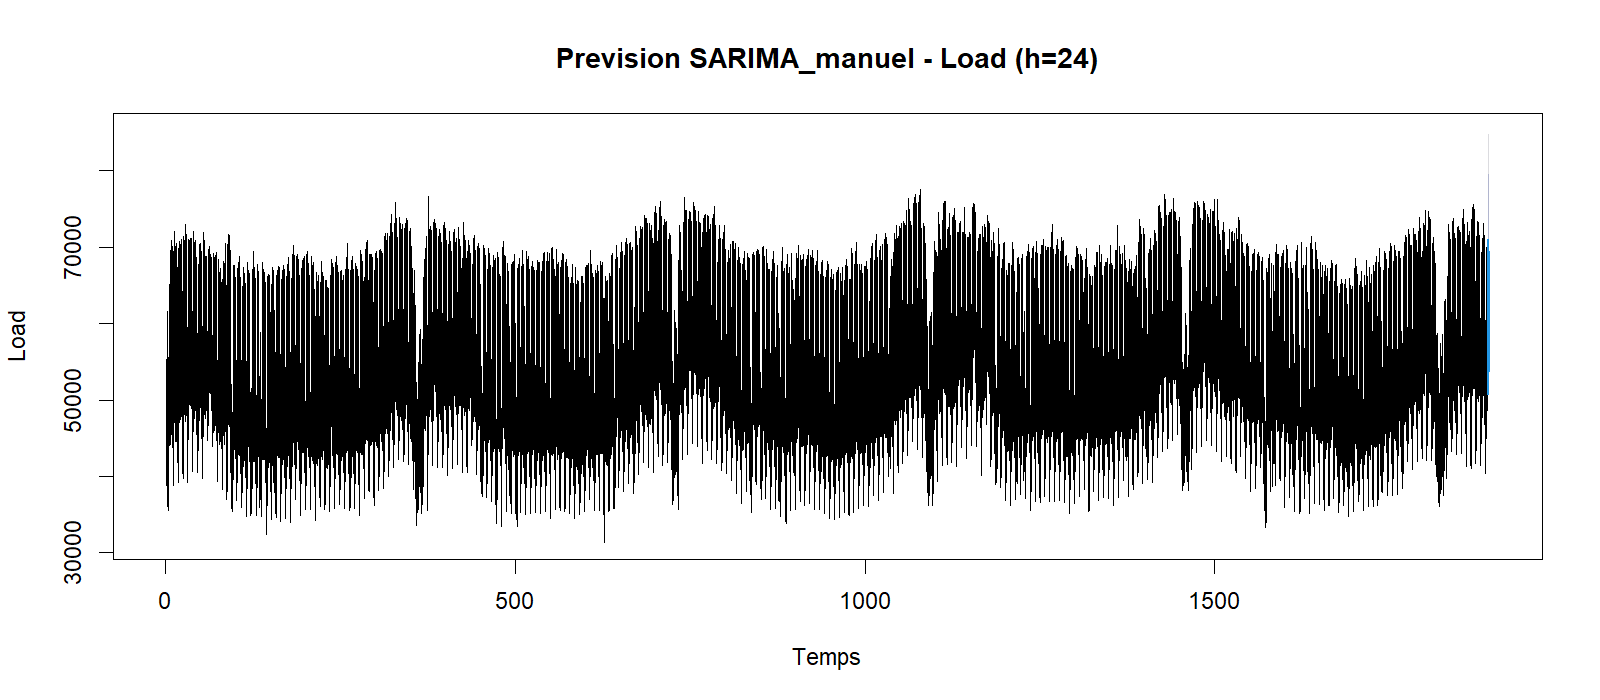
\includegraphics[width=0.9\textwidth]{R_prev_Load.png}
\caption{Prévision \texttt{Load} à \(h=24\) (modèle retenu, R).}
\label{fig:prev_r_load}
\end{figure}

\begin{figure}[H]
\centering
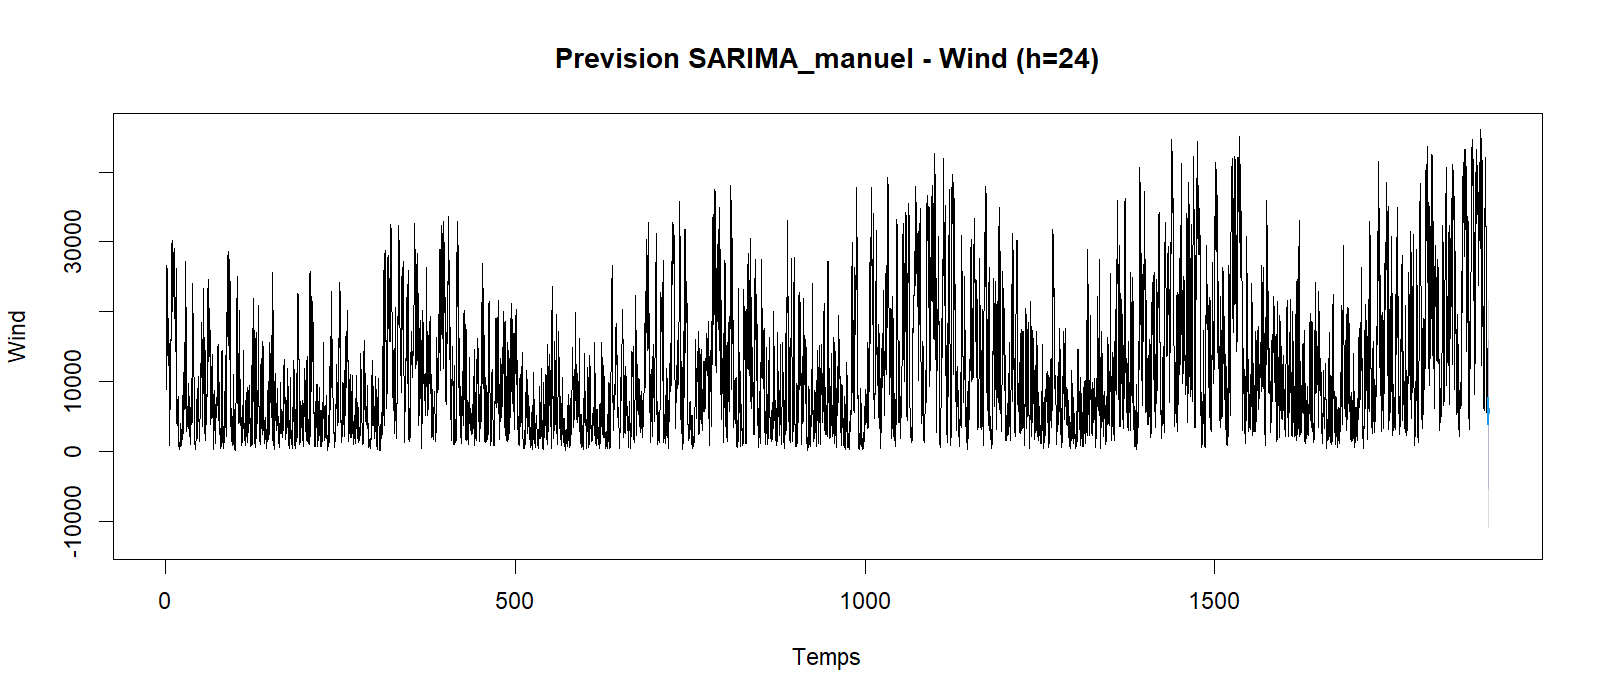
\includegraphics[width=0.9\textwidth]{R_prev_Wind.png}
\caption{Prévision \texttt{Wind} à \(h=24\) (R).}
\label{fig:prev_r_wind}
\end{figure}

\begin{figure}[H]
\centering
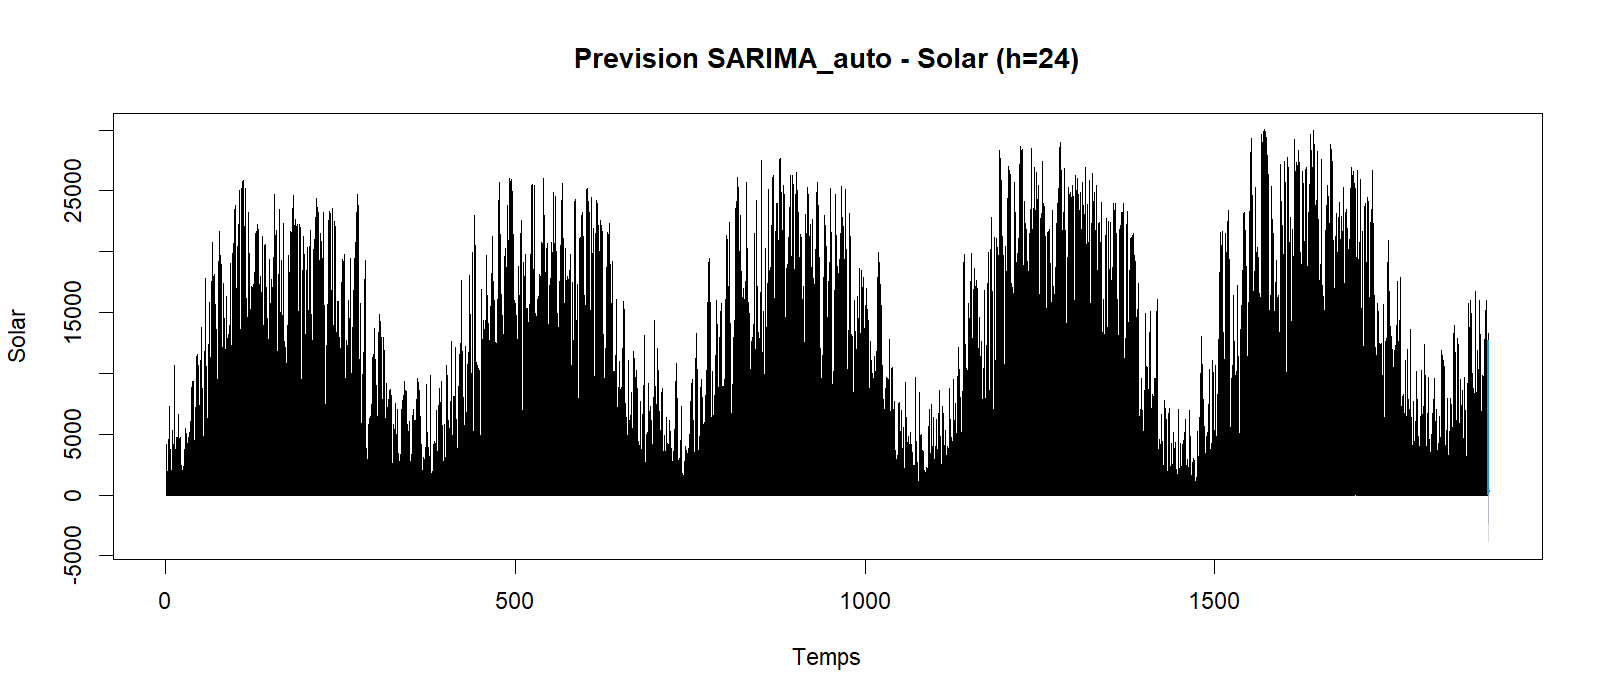
\includegraphics[width=0.9\textwidth]{R_prev_Solar.png}
\caption{Prévision \texttt{Solar} à \(h=24\) (R).}
\label{fig:prev_r_solar}
\end{figure}

\begin{figure}[H]
\centering
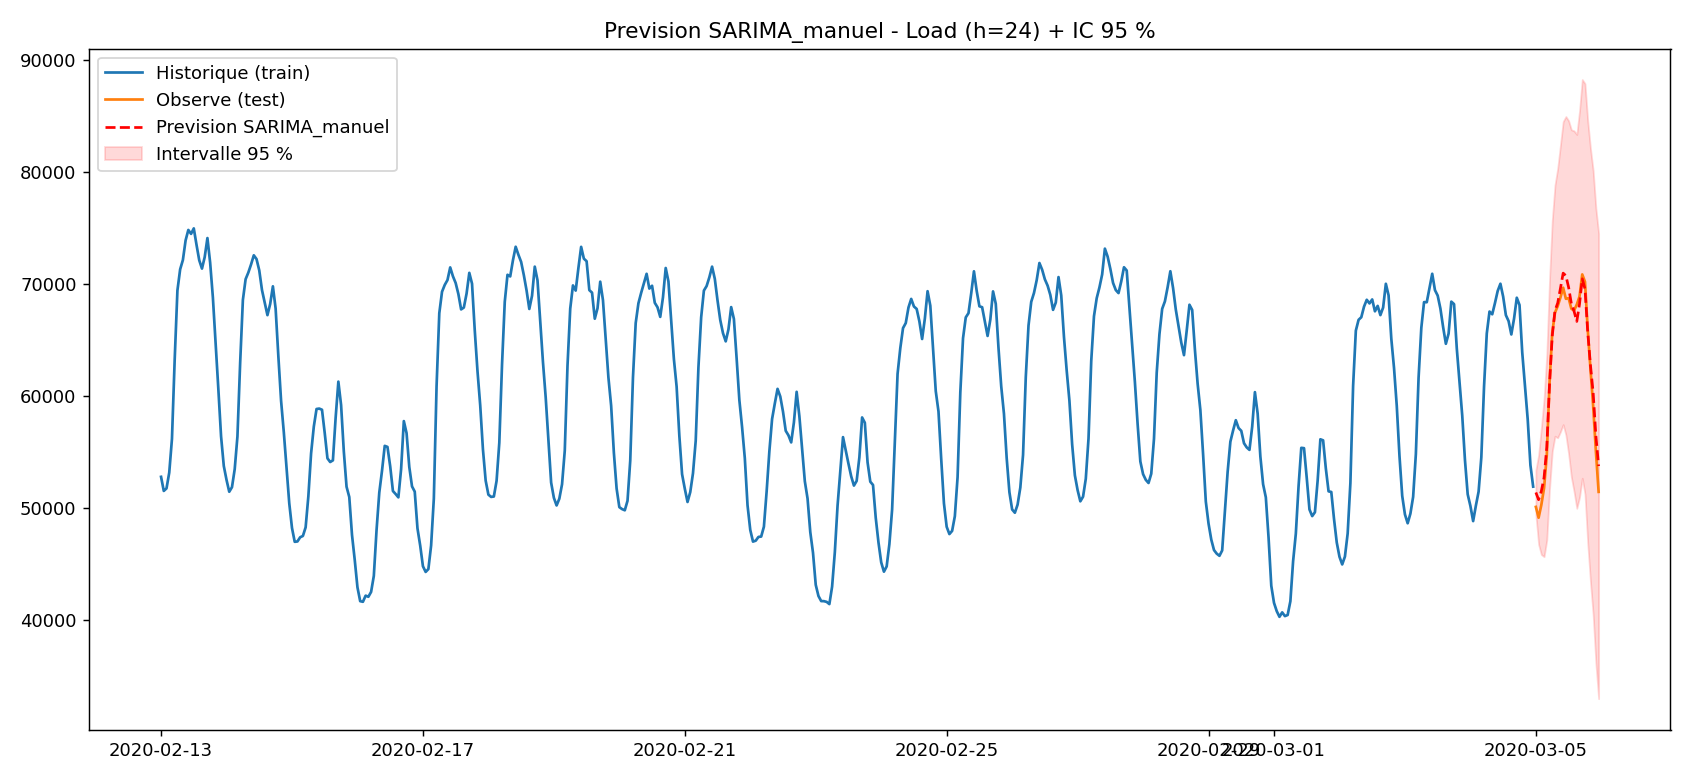
\includegraphics[width=0.9\textwidth]{py_prev_Load.png}
\caption{Prévision \texttt{Load} (Python) --- cohérente avec R.}
\label{fig:prev_py_load}
\end{figure}

\begin{figure}[H]
\centering
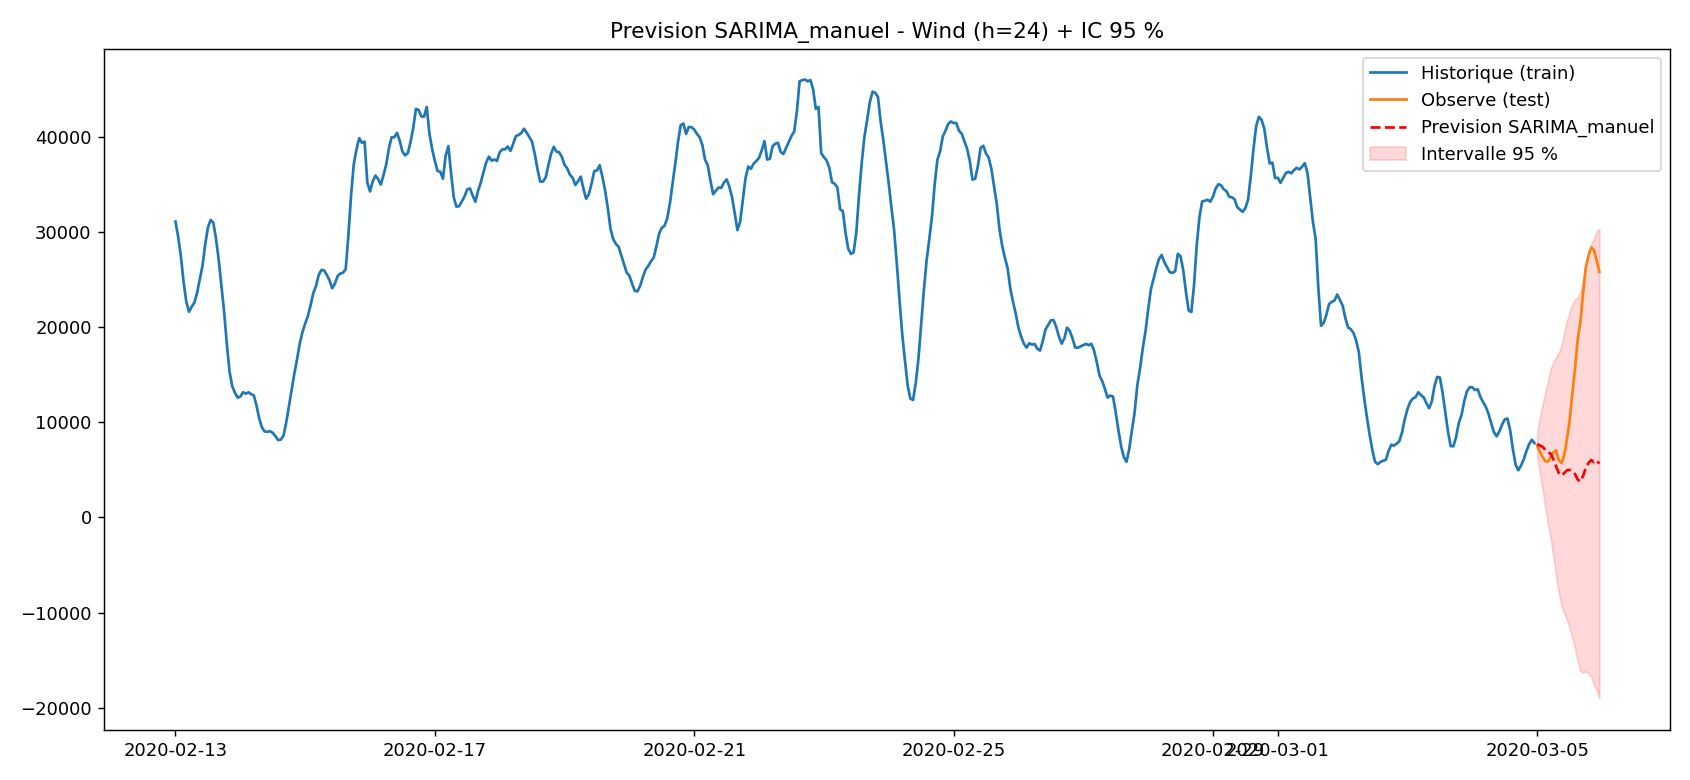
\includegraphics[width=0.9\textwidth]{py_prev_Wind.png}
\caption{Prévision \texttt{Wind} (Python).}
\label{fig:prev_py_wind}
\end{figure}

\begin{figure}[H]
\centering
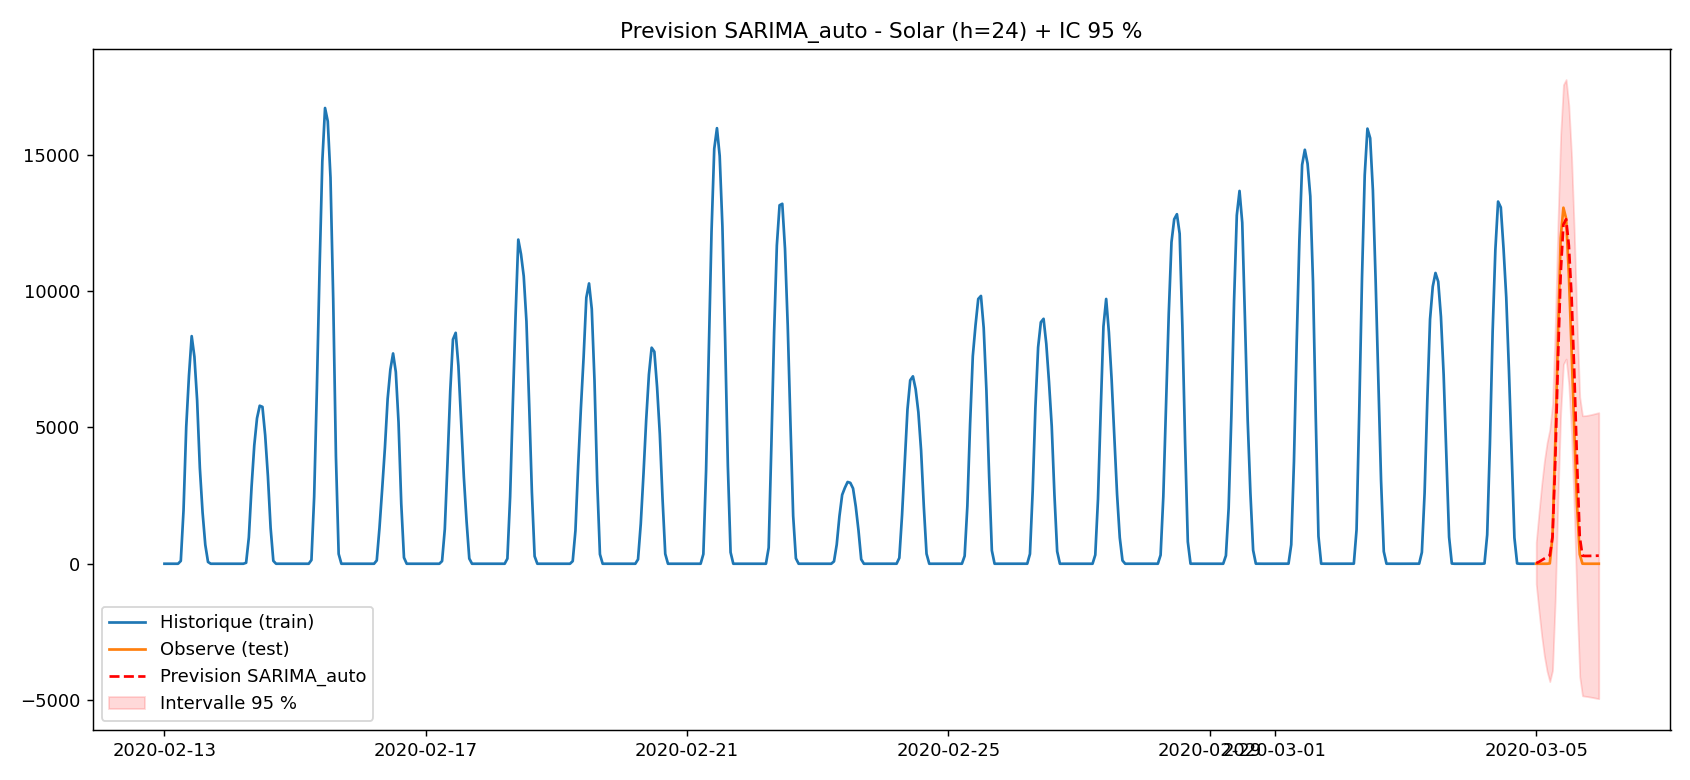
\includegraphics[width=0.9\textwidth]{py_prev_Solar.png}
\caption{Prévision \texttt{Solar} (Python).}
\label{fig:prev_py_solar}
\end{figure}

\begin{figure}[H]
\centering
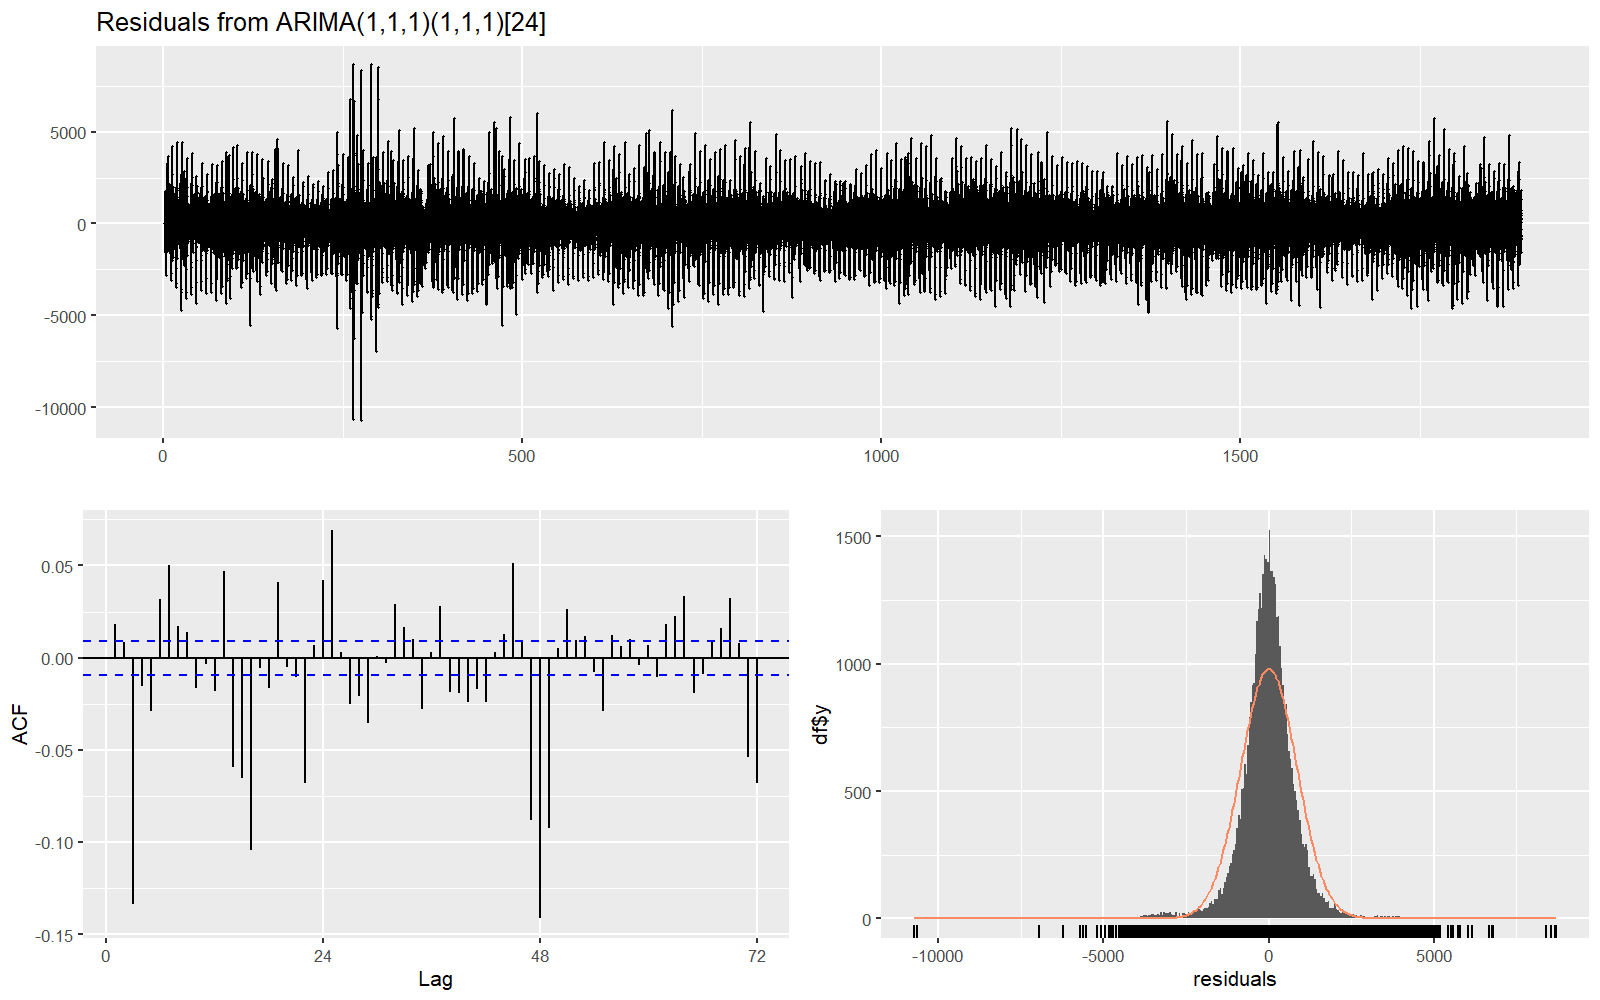
\includegraphics[width=0.9\textwidth]{R_resid_Load.png}
\caption{Diagnostic des résidus \texttt{Load} (R).}
\label{fig:resid_r_load}
\end{figure}

\begin{figure}[H]
\centering
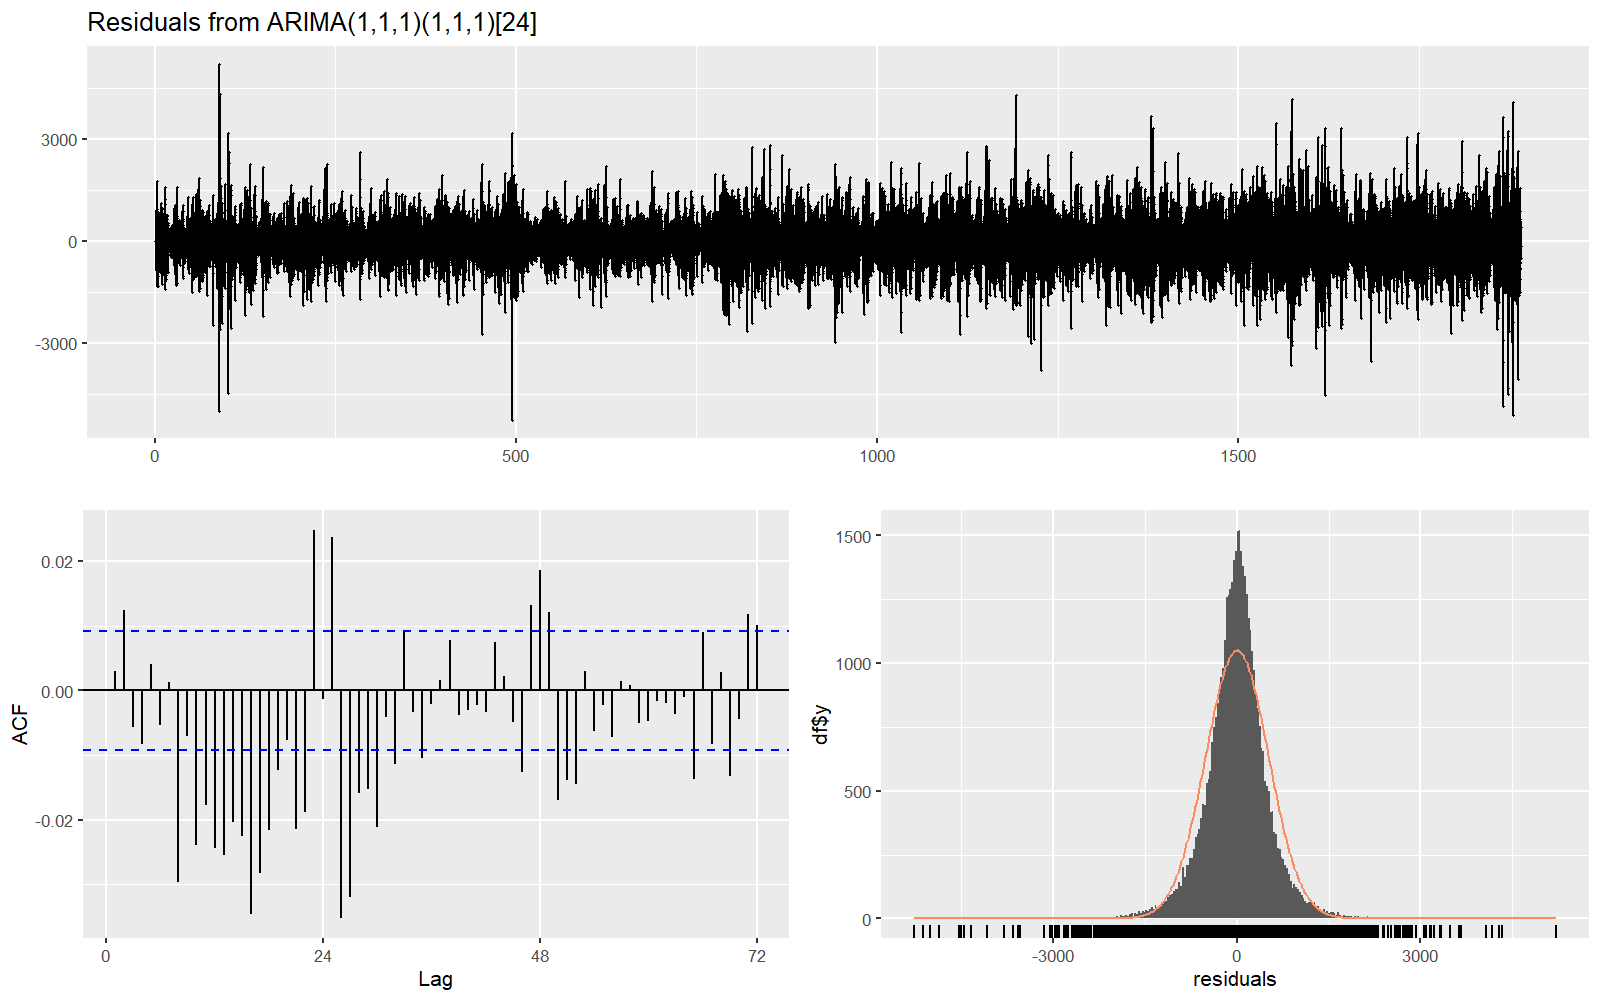
\includegraphics[width=0.9\textwidth]{R_resid_Wind.png}
\caption{Diagnostic des résidus \texttt{Wind} (R).}
\label{fig:resid_r_wind}
\end{figure}

\begin{figure}[H]
\centering
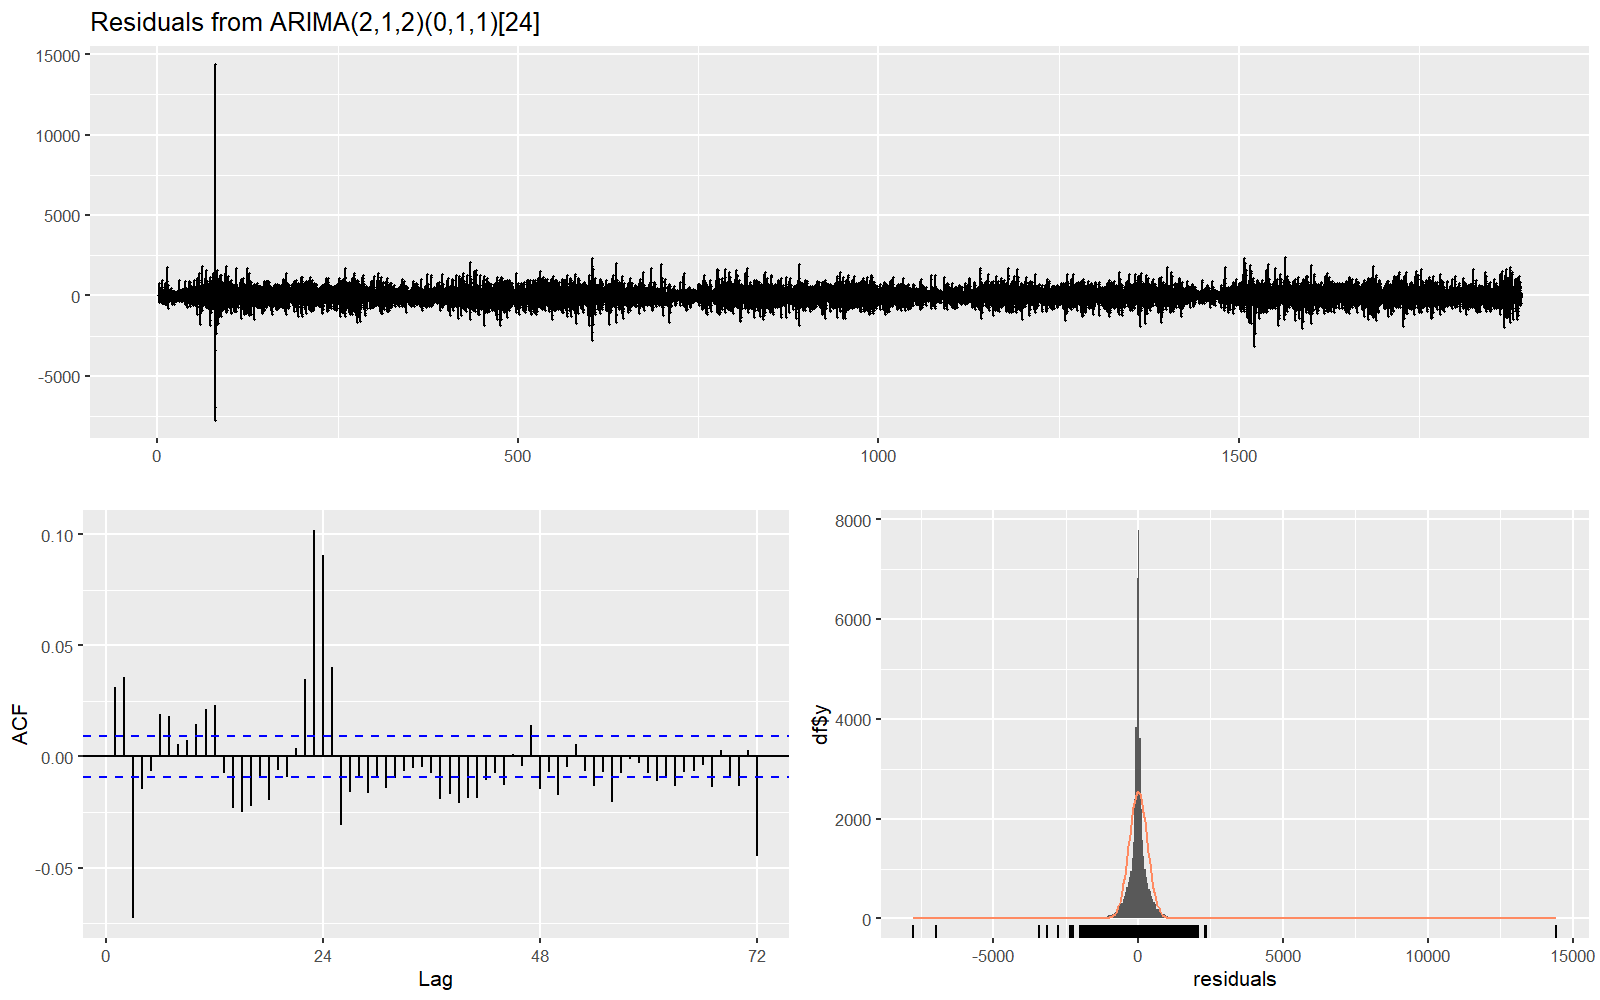
\includegraphics[width=0.9\textwidth]{R_resid_Solar.png}
\caption{Diagnostic des résidus \texttt{Solar} (R).}
\label{fig:resid_r_solar}
\end{figure}

\begin{figure}[H]
\centering
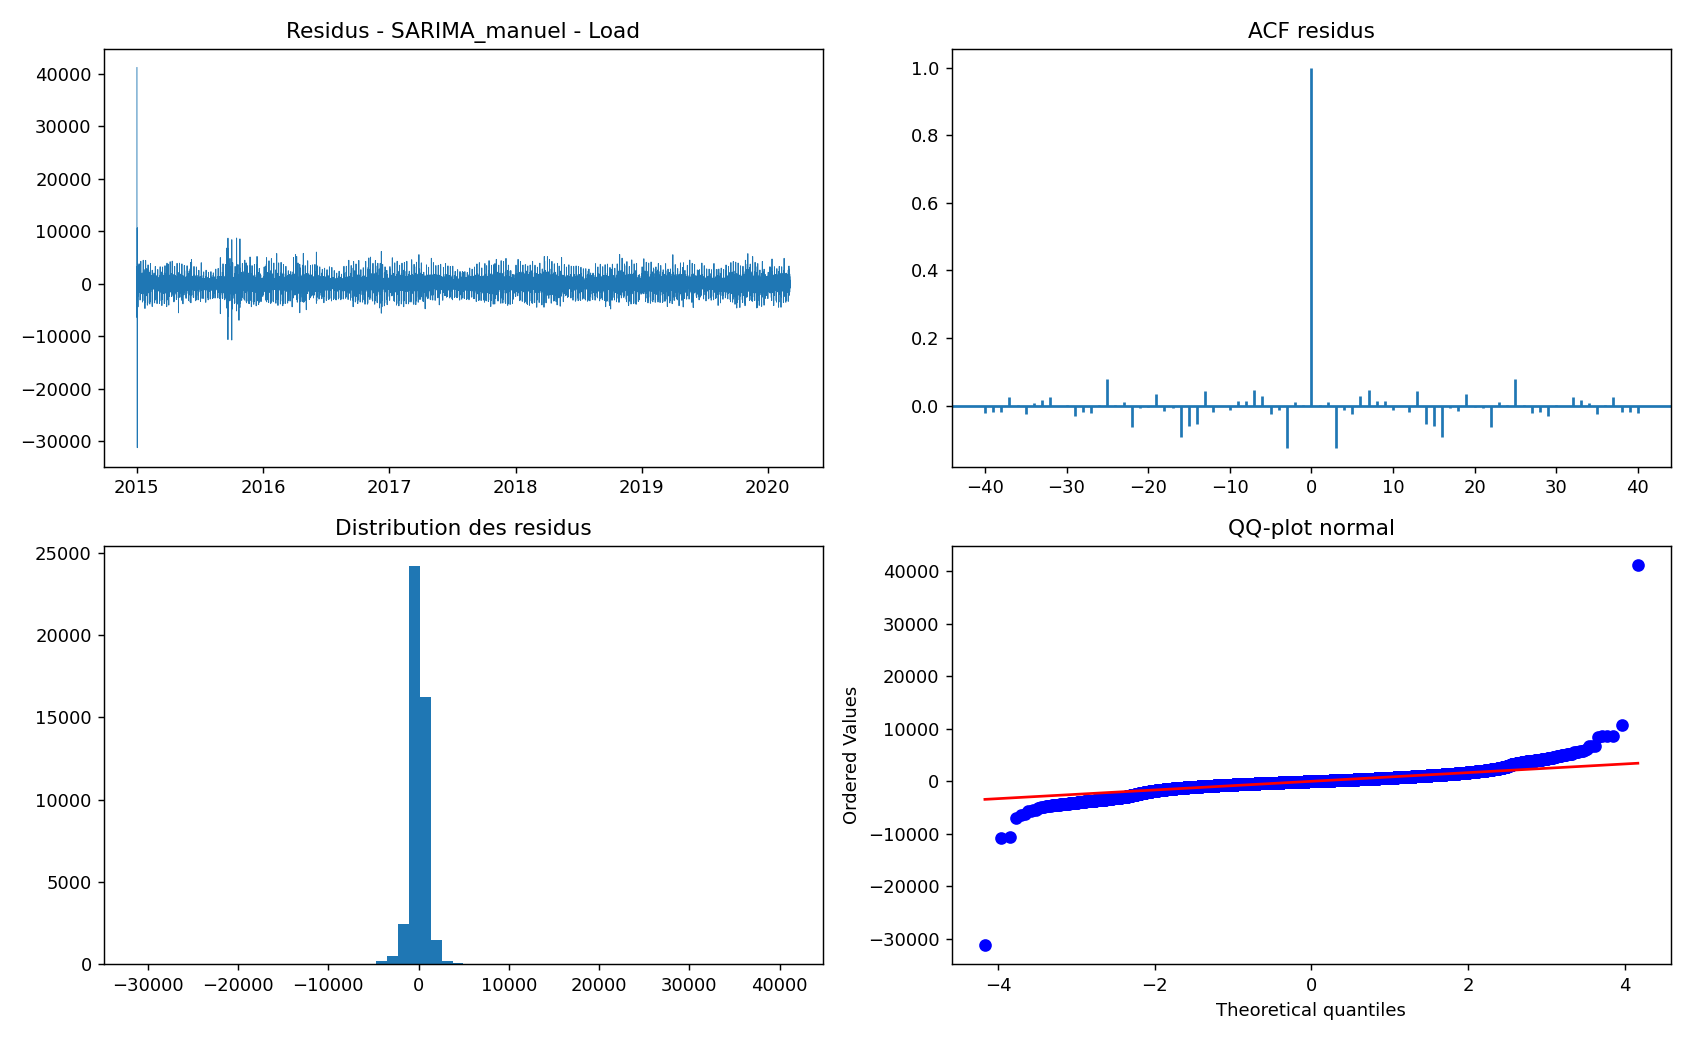
\includegraphics[width=0.9\textwidth]{py_resid_Load.png}
\caption{Diagnostic des résidus \texttt{Load} (Python).}
\label{fig:resid_py_load}
\end{figure}

\begin{figure}[H]
\centering
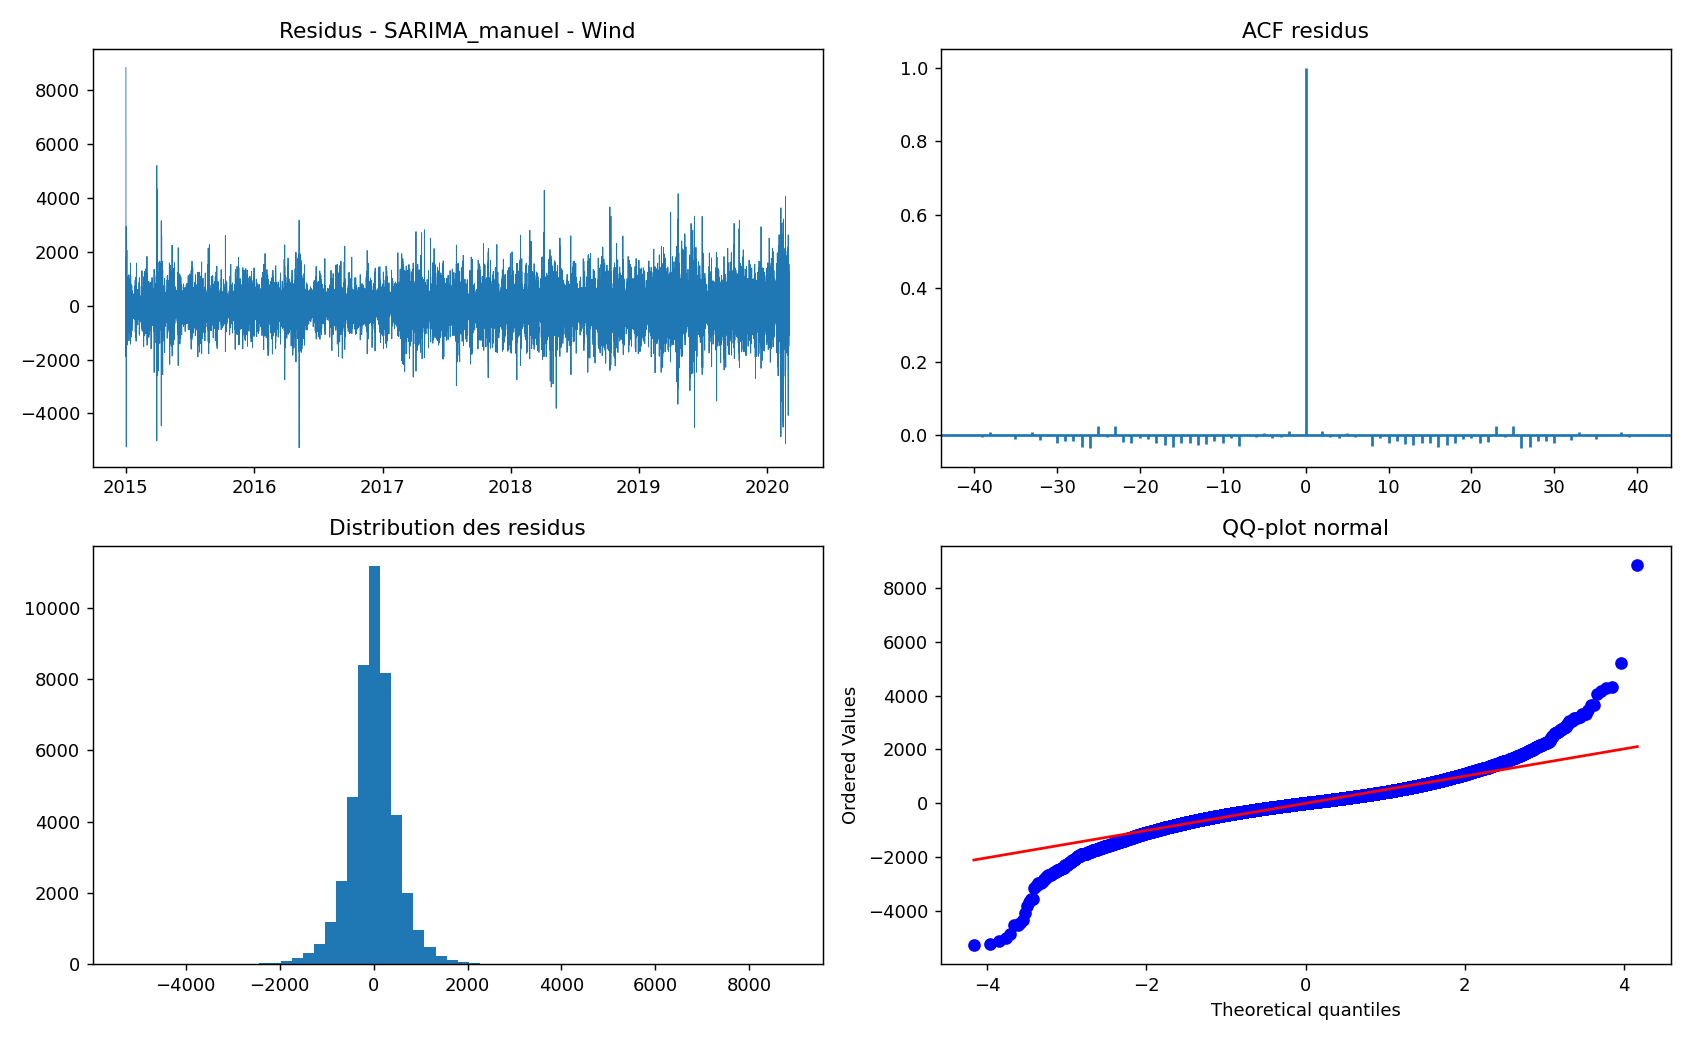
\includegraphics[width=0.9\textwidth]{py_resid_Wind.png}
\caption{Diagnostic des résidus \texttt{Wind} (Python).}
\label{fig:resid_py_wind}
\end{figure}

\begin{figure}[H]
\centering
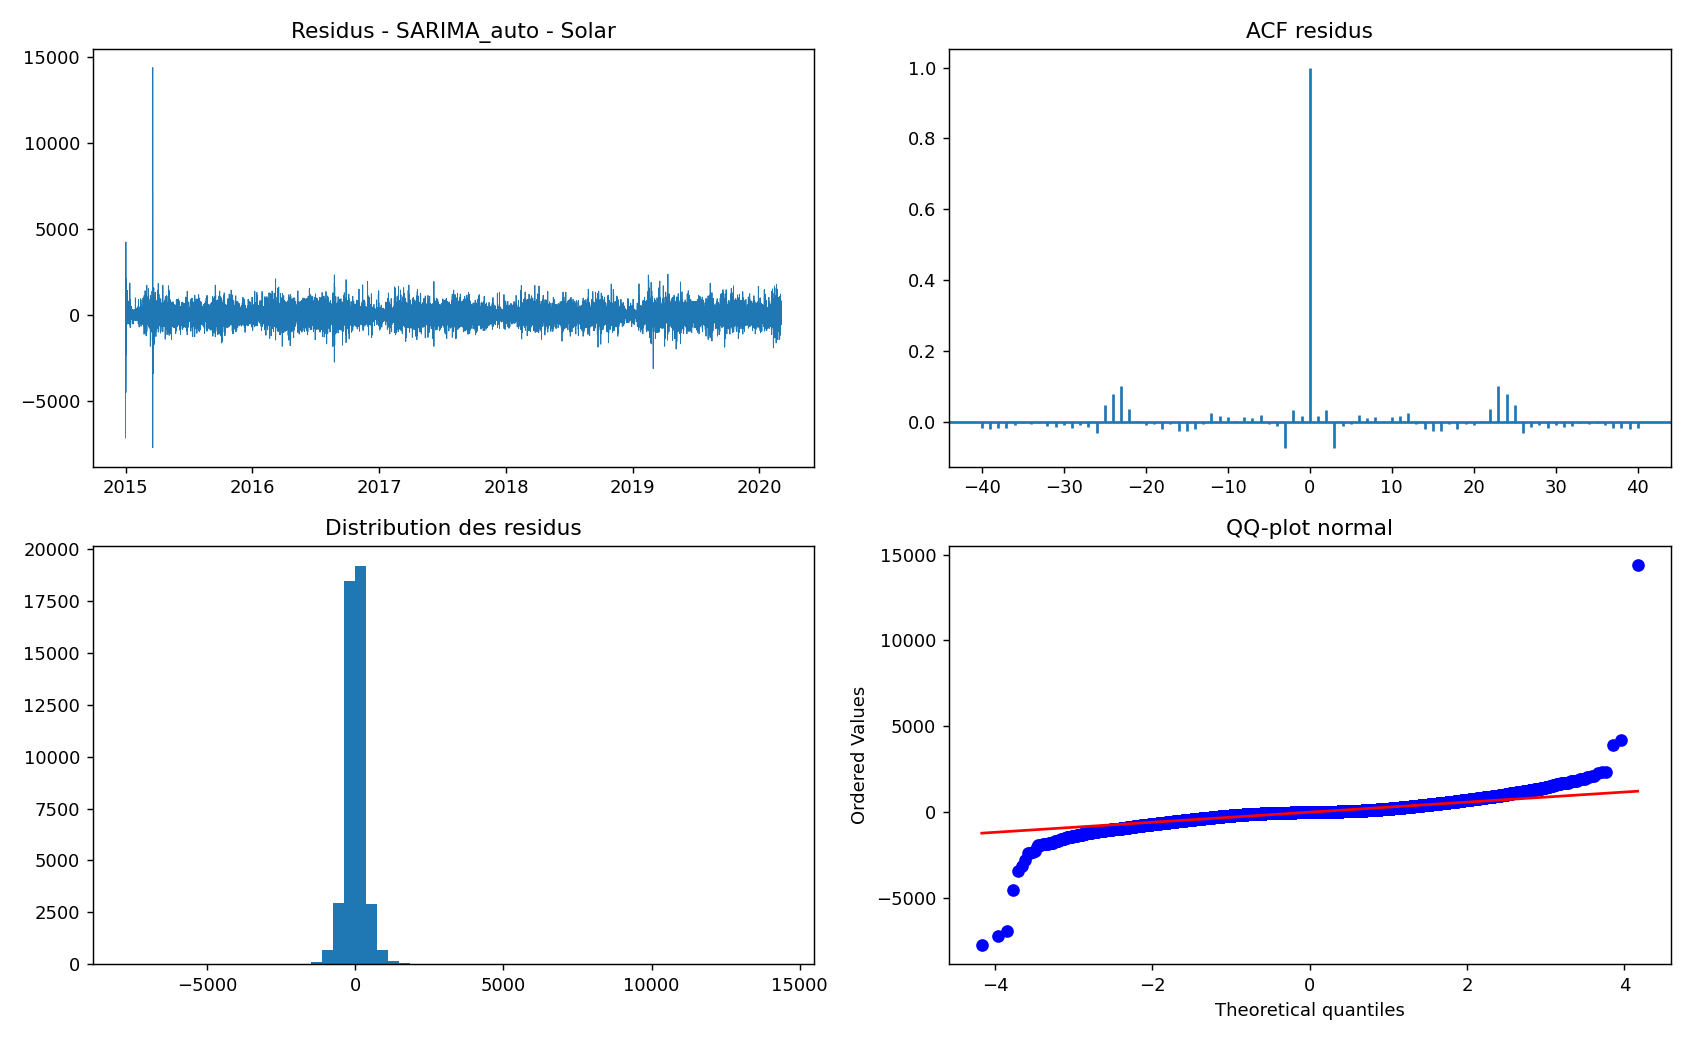
\includegraphics[width=0.9\textwidth]{py_resid_Solar.png}
\caption{Diagnostic des résidus \texttt{Solar} (Python).}
\label{fig:resid_py_solar}
\end{figure}

\FloatBarrier

\subsection{Liaisons dynamiques : VAR, Granger, Johansen, VECM}

\subsubsection{Sélection de l'ordre du VAR}
Le tableau~\ref{tab:var_order} (extrait de
\texttt{R\_var\_order.csv}) montre que le critère AIC atteint son minimum à
\(p=14\) (sur les moyennes journalières différenciées), retenu pour la suite.
Les critères HQ/SC suggèrent un ordre plus faible, mais l'AIC est privilégié
pour ne pas sous-paramétrer la dynamique. Python aboutit au même ordre
(\texttt{py\_var\_order.csv}).

\begin{table}[H]
\centering
\caption{Critères d'information pour la sélection de l'ordre du VAR (R).
Source : \texttt{R\_var\_order.csv}.}
\label{tab:var_order}
\small
\begin{tabular}{lrrrrrrrr}
\toprule
Critère & 10 & 11 & 12 & 13 & \textbf{14} & 15 \\
\midrule
AIC & 47{,}540 & 47{,}534 & 47{,}510 & 47{,}432 & \textbf{47{,}375} & 47{,}378 \\
HQ  & 47{,}641 & 47{,}645 & 47{,}631 & 47{,}563 & \textbf{47{,}516} & 47{,}528 \\
SC  & 47{,}815 & 47{,}835 & 47{,}838 & 47{,}787 & \textbf{47{,}757} & 47{,}786 \\
FPE & 4{,}43e20 & 4{,}40e20 & 4{,}30e20 & 3{,}98e20 & \textbf{3{,}76e20} & 3{,}77e20 \\
\bottomrule
\end{tabular}
\end{table}

\subsubsection{Causalité de Granger}
Le tableau~\ref{tab:granger} teste les six relations ordonnées. Seule
l'hypothèse \(\texttt{Wind} \to \texttt{Load}\) est rejetée (R : \(p=0{,}013\)
; Python : \(p=0{,}002\)), c'est-à-dire que la production éolienne
\textbf{cause} la consommation au sens de Granger. Aucune des autres
directions n'est significative.

\begin{table}[H]
\centering
\caption{Test de causalité de Granger (R et Python).
Sources : \texttt{R\_granger.csv}, \texttt{py\_granger.csv}.}
\label{tab:granger}
\small
\begin{tabular}{lrrl}
\toprule
Hypothèse & $p$ (R) & $p$ (py) & Conclusion \\
\midrule
\texttt{Wind} $\to$ \texttt{Load}  & \textbf{0{,}0126} & \textbf{0{,}0022} & Oui (rejet H0) \\
\texttt{Solar} $\to$ \texttt{Load} & 0{,}767 & 0{,}256 & Non \\
\texttt{Load} $\to$ \texttt{Wind}  & 0{,}244 & 0{,}157 & Non \\
\texttt{Solar} $\to$ \texttt{Wind} & 0{,}371 & 0{,}339 & Non \\
\texttt{Load} $\to$ \texttt{Solar}& 0{,}738 & 0{,}752 & Non \\
\texttt{Wind} $\to$ \texttt{Solar}& 0{,}099 & 0{,}058 & Non \\
\bottomrule
\end{tabular}
\end{table}

\subsubsection{Cointégration de Johansen et VECM}
Le test de trace de Johansen (tableau~\ref{tab:johansen}) conduit à
\textbf{\(r=2\)} relations de cointégration : au premier rang, la statistique
(\(155{,}32\)) dépasse largement la valeur critique (\(34{,}91\)) ; au second
rang (\(58{,}54\)) elle dépasse encore \(19{,}96\) ; au troisième rang
(\(8{,}67\)) elle passe sous \(9{,}24\). Ce résultat est \textbf{identique} en
R et en Python.

\begin{table}[H]
\centering
\caption{Test de trace de Johansen (valeurs critiques à 95\,\%).
Sources : \texttt{R\_johansen.csv}, \texttt{py\_johansen.csv}.}
\label{tab:johansen}
\small
\begin{tabular}{lrrrr}
\toprule
Rang testé & Stat. (R) & Stat. (py) & CV 95\,\% & Conclusion \\
\midrule
$r=0$ & 152{,}97 & 155{,}32 & 34{,}91 & Rejet $r=0$ \\
$r\leq 1$ & 57{,}83 & 58{,}54 & 19{,}96 & Rejet $r\leq 1$ \\
$r\leq 2$ & 8{,}66 & 8{,}67 & 9{,}24 & Non rejeté \\
\bottomrule
\end{tabular}
\end{table}

Le VECM estimé (tableaux~\ref{tab:vecm} et~\ref{tab:vecm_alpha}) fournit des
vecteurs de cointégration \(\beta\) normalisés très proches en R et Python
(\texttt{Solar} : \(\approx 0{,}91\) et \(\approx 1{,}22\) sur les deux
relations) et des vitesses d'ajustement \(\alpha\) cohérentes : la charge et
l'éolien présentent une force de rappel significative
(\(\alpha \approx -0{,}24\) pour \texttt{Load} dans l'équation 1 et
\texttt{Wind} dans l'équation 2), tandis que le solaire s'ajuste très peu.

\begin{table}[H]
\centering
\caption{Vecteurs de cointégration normalisés $\beta$ du VECM
(\(r=2\)). Sources : \texttt{R\_vecm.csv}, \texttt{py\_vecm.csv}.}
\label{tab:vecm}
\small
\begin{tabular}{lrr}
\toprule
Variable (lag 1) & ECT\_1 & ECT\_2 \\
\midrule
\texttt{Load}  & 1{,}0000 & 0{,}0000 \\
\texttt{Wind}  & 0{,}0000 & 1{,}0000 \\
\texttt{Solar} & 0{,}9084 (py 0{,}9148) & 1{,}2126 (py 1{,}2222) \\
Constante      & $-59\,819$ (py $-59\,848$) & $-16\,705$ (py $-16\,780$) \\
\bottomrule
\end{tabular}
\end{table}

\begin{table}[H]
\centering
\caption{Vitesses d'ajustement $\alpha$ du VECM.
Sources : \texttt{R\_vecm\_alpha.csv}, \texttt{py\_vecm\_alpha.csv}.}
\label{tab:vecm_alpha}
\small
\begin{tabular}{lrrr}
\toprule
Équation & $\Delta$\texttt{Load} & $\Delta$\texttt{Wind} & $\Delta$\texttt{Solar} \\
\midrule
ECT\_1 & $-0{,}2379$ & $0{,}1196$ & $0{,}0030$ \\
ECT\_2 & $0{,}0161$ & $-0{,}2396$ & $0{,}0063$ \\
\bottomrule
\end{tabular}
\end{table}

\subsubsection{Diagnostics du VAR}
Le tableau~\ref{tab:var_diag} indique le rejet des trois tests : le VAR
journalier laisse une autocorrélation, une non-normalité et surtout un effet
\textbf{ARCH multivarié}, ce qui confirme une nouvelle fois le besoin d'une
modélisation explicite de la volatilité.

\begin{table}[H]
\centering
\caption{Diagnostics multivariés du VAR. Sources :
\texttt{R\_var\_diagnostics.csv}, \texttt{py\_var\_diagnostics.csv}.}
\label{tab:var_diag}
\small
\begin{tabular}{lrr}
\toprule
Test & $p$ (R) & $p$ (py) \\
\midrule
Portmanteau (autocorrélation) & $<0{,}001$ & $5{,}0\text{e-}40$ \\
Normalité multivariée (JB) & $<0{,}001$ & $<0{,}001$ \\
ARCH multivarié (Load) & $<0{,}001$ & $1{,}1\text{e-}24$ \\
ARCH multivarié (Wind) & --- & $2{,}6\text{e-}16$ \\
ARCH multivarié (Solar) & --- & $4{,}6\text{e-}15$ \\
\bottomrule
\end{tabular}
\end{table}

\subsubsection{Réponse impulsionnelle et décomposition de la variance}
Les figures~\ref{fig:irf_r} et~\ref{fig:fevd_r} (et leurs homologues Python
\ref{fig:irf_py} et~\ref{fig:fevd_py}) synthétisent les dynamiques. La
décomposition de variance à \(28\) jours (tableau~\ref{tab:fevd_summary})
montre que chaque série est essentiellement expliquée par elle-même
(\(92\) à \(97\,\%\)), avec une contribution de \texttt{Wind} à \texttt{Load}
d'environ \(2{,}2\,\%\) et de \texttt{Solar} à \texttt{Load} d'environ
\(4{,}1\,\%\) --- cohérent avec la causalité de Granger détectée.

\begin{figure}[H]
\centering
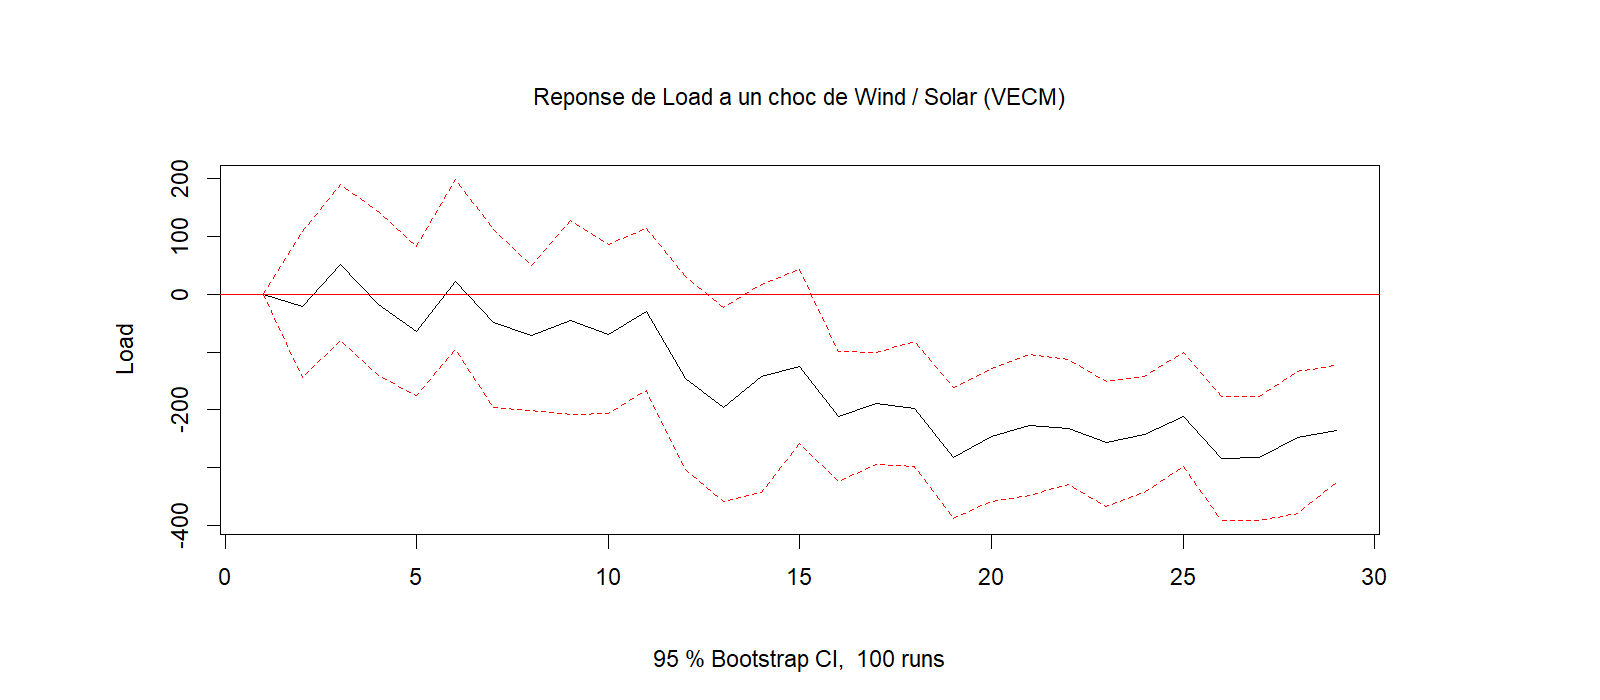
\includegraphics[width=0.9\textwidth]{R_var_irf_load.png}
\caption{Réponse de \texttt{Load} à un choc de \texttt{Wind}/\texttt{Solar} (R, 28 jours).}
\label{fig:irf_r}
\end{figure}

\begin{figure}[H]
\centering
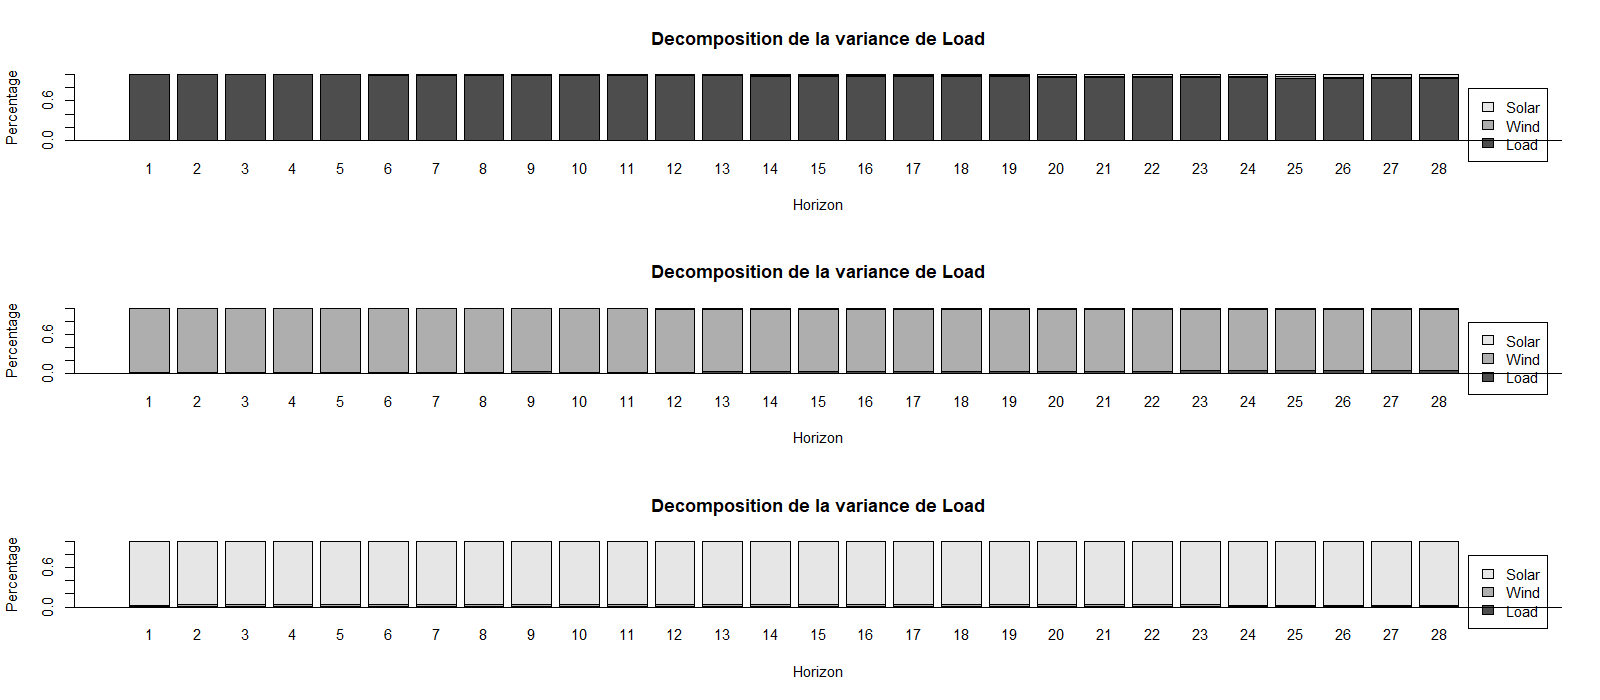
\includegraphics[width=0.9\textwidth]{R_var_fevd_load.png}
\caption{Décomposition de la variance de \texttt{Load} (R).}
\label{fig:fevd_r}
\end{figure}

\begin{figure}[H]
\centering
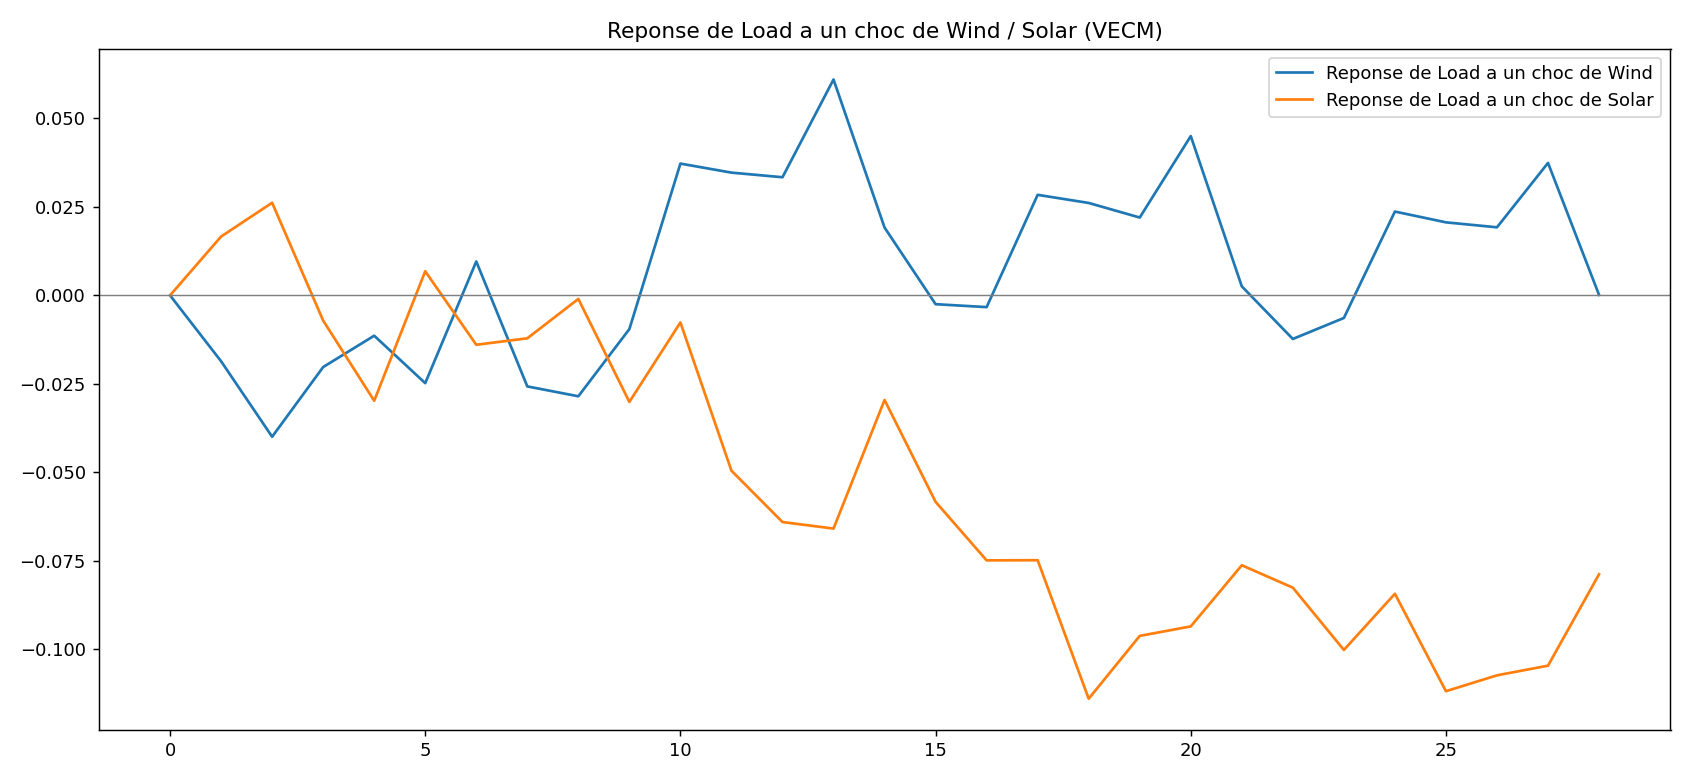
\includegraphics[width=0.9\textwidth]{py_var_irf_load.png}
\caption{Réponse de \texttt{Load} à un choc (Python).}
\label{fig:irf_py}
\end{figure}

\begin{figure}[H]
\centering
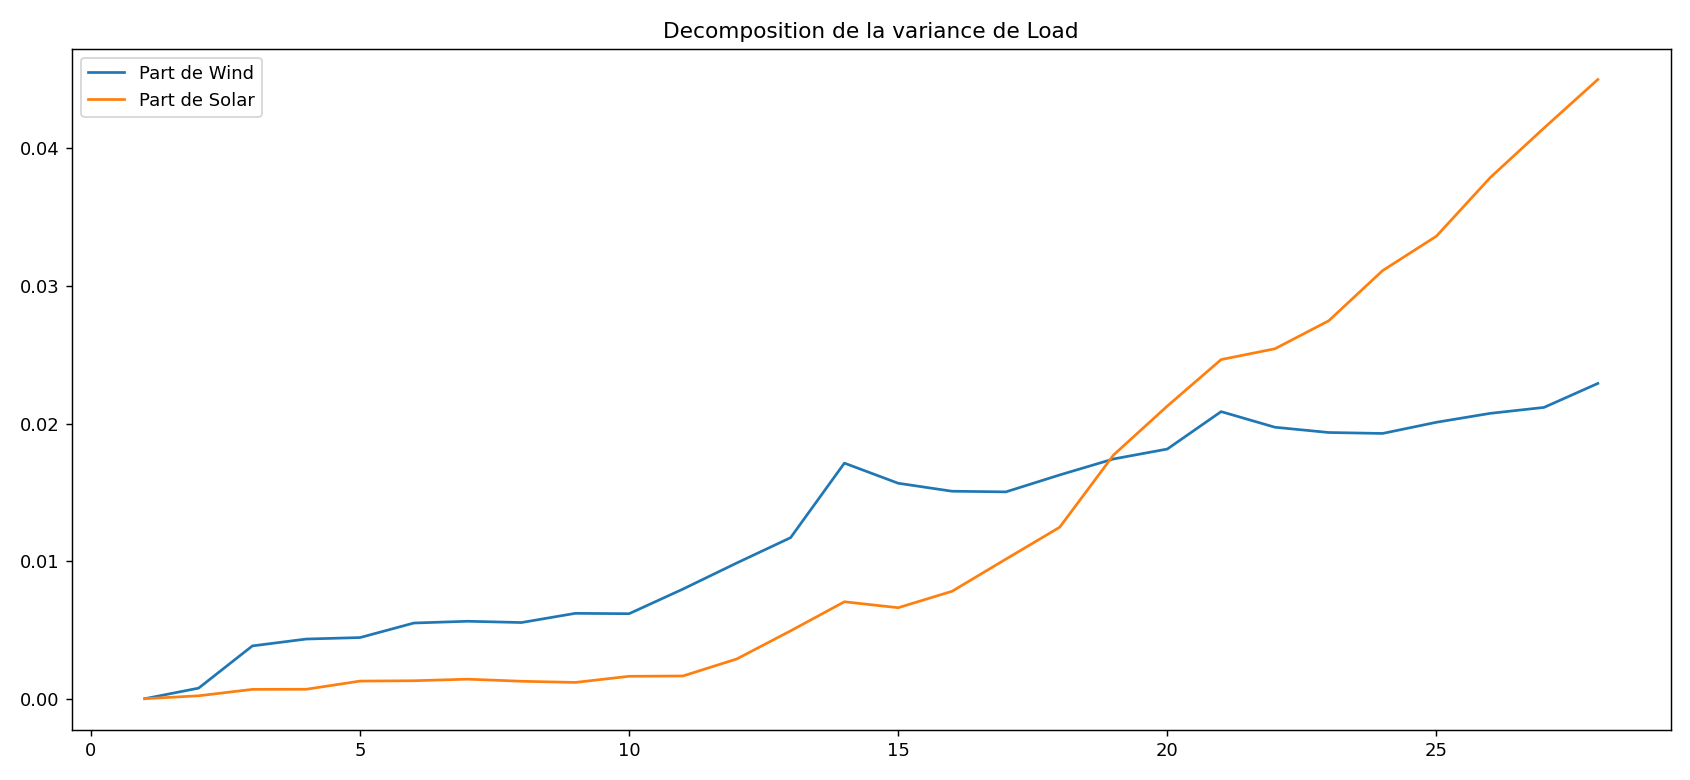
\includegraphics[width=0.9\textwidth]{py_var_fevd_load.png}
\caption{Décomposition de la variance de \texttt{Load} (Python).}
\label{fig:fevd_py}
\end{figure}

\begin{table}[H]
\centering
\caption{Décomposition de la variance au jour 28 (R).
Source : \texttt{R\_var\_fevd.csv}.}
\label{tab:fevd_summary}
\small
\begin{tabular}{lrrr}
\toprule
Variable expliquée & Part \texttt{Load} & Part \texttt{Wind} & Part \texttt{Solar} \\
\midrule
\texttt{Load}  & 0{,}9368 & 0{,}0219 & 0{,}0413 \\
\texttt{Wind}  & 0{,}0459 & 0{,}9243 & 0{,}0298 \\
\texttt{Solar} & 0{,}0080 & 0{,}0213 & 0{,}9708 \\
\bottomrule
\end{tabular}
\end{table}

\FloatBarrier

\subsection{Modélisation de la volatilité : ARCH / GARCH}
\label{sec:garch}

\subsubsection{Persistance de la volatilité}
Le tableau~\ref{tab:garch_pers_r} (R) et le tableau~\ref{tab:garch_pers_py}
(Python) résument la persistance. Pour \texttt{Wind}, les trois spécifications
sont covariation-stationnaires avec une persistance très élevée
(\(\approx 0{,}99\)), soit une demi-vie de \(68\) (GARCH(1,1)) à \(675\)
(EGARCH) jours. Pour \texttt{Load}, GARCH(1,1) est proche de la frontière
(persistance \(\approx 0{,}998\) en R). Pour \texttt{Solar}, GARCH(1,1) et
GARCH(2,1) sont non stationnaires (persistance \(\geq 1\)), seul
l'EGARCH(1,1) reste stable (\(\approx 0{,}99\)).

\begin{table}[H]
\centering
\caption{Persistance de la volatilité (R).
Source : \texttt{R\_garch\_persistence.csv}.}
\label{tab:garch_pers_r}
\small
\begin{tabular}{llrrl}
\toprule
Variable & Modèle & Persistance & Demi-vie (j) & Cov. stationnaire \\
\midrule
\texttt{Load}  & GARCH(1,1)  & 0{,}9981 & 366{,}8 & Oui \\
\texttt{Load}  & GARCH(2,1)  & 0{,}4540 & 0{,}9 & Oui \\
\texttt{Load}  & EGARCH(1,1) & 0{,}6312 & 1{,}5 & Oui \\
\texttt{Wind}  & GARCH(1,1)  & 0{,}9899 & 68{,}5 & Oui \\
\texttt{Wind}  & GARCH(2,1)  & 0{,}9875 & 55{,}3 & Oui \\
\texttt{Wind}  & EGARCH(1,1) & 0{,}9990 & 675{,}2 & Oui \\
\texttt{Solar} & GARCH(1,1)  & 1{,}0050 & NA & Non \\
\texttt{Solar} & GARCH(2,1)  & 1{,}0051 & NA & Non \\
\texttt{Solar} & EGARCH(1,1) & 0{,}9936 & 108{,}3 & Oui \\
\bottomrule
\end{tabular}
\end{table}

\begin{table}[H]
\centering
\caption{Persistance de la volatilité (Python).
Source : \texttt{py\_garch\_persistence.csv}.}
\label{tab:garch_pers_py}
\small
\begin{tabular}{llrrl}
\toprule
Variable & Modèle & Persistance & Demi-vie (j) & Convergence \\
\midrule
\texttt{Load}  & GARCH(1,1)  & --- & --- & Non \\
\texttt{Load}  & GARCH(2,1)  & 0{,}8222 & 3{,}5 & Oui \\
\texttt{Load}  & EGARCH(1,1) & --- & --- & Non \\
\texttt{Wind}  & GARCH(1,1)  & 0{,}9905 & 72{,}7 & Oui \\
\texttt{Wind}  & GARCH(2,1)  & 0{,}9892 & 63{,}6 & Oui \\
\texttt{Wind}  & EGARCH(1,1) & 0{,}9861 & 49{,}3 & Oui \\
\texttt{Solar} & GARCH(1,1)  & 1{,}0000 & --- & Non \\
\texttt{Solar} & GARCH(2,1)  & 1{,}0000 & --- & Non \\
\texttt{Solar} & EGARCH(1,1) & 0{,}9894 & 65{,}0 & Oui \\
\bottomrule
\end{tabular}
\end{table}

\subsubsection{Coefficients estimés}
Le tableau~\ref{tab:garch_coef_py} détaille les coefficients estimés en
Python (avec AIC/BIC et paramètre de queue lourde \(\nu_t\)). On note pour
\texttt{Wind} un \(\beta_1 \approx 0{,}935\) (persistance de la volatilité) et
pour \texttt{Solar} un \(\nu_t \approx 8{,}7\), confirmant des queues plus
épaisses que la normale.

\begin{table}[H]
\centering
\caption{Coefficients GARCH estimés (Python).
Source : \texttt{py\_garch\_coefficients.csv}.}
\label{tab:garch_coef_py}
\small
\begin{tabular}{llrrrrrr}
\toprule
Variable & Modèle & $\mu$ & $\omega$ & $\alpha_1$ & $\beta_1$ & Pers. & $\nu_t$ \\
\midrule
\texttt{Load}  & GARCH(2,1)  & $-0{,}186$ & 1{,}296 & 0{,}0013 & 0{,}8209 & 0{,}822 & 2{,}05 \\
\texttt{Wind}  & GARCH(1,1)  & $-0{,}004$ & 0{,}0113 & 0{,}0553 & 0{,}9352 & 0{,}991 & 7{,}35 \\
\texttt{Wind}  & EGARCH(1,1) & $-0{,}005$ & 0{,}0039 & 0{,}1205 & 0{,}9861 & 0{,}986 & 7{,}33 \\
\texttt{Solar} & GARCH(1,1)  & $-0{,}001$ & 0{,}0042 & 0{,}0890 & 0{,}9110 & 1{,}000 & 8{,}72 \\
\texttt{Solar} & EGARCH(1,1) & $0{,}000$  & 0{,}0056 & 0{,}1942 & 0{,}9894 & 0{,}989 & 8{,}09 \\
\bottomrule
\end{tabular}
\end{table}

\subsubsection{Diagnostics GARCH et volatilité conditionnelle}
Le tableau~\ref{tab:garch_diag} montre que les résidus standardisés du
GARCH(1,1) ne sont plus autocorrélés (Ljung--Box des résidus) et que, pour
\texttt{Solar}, les résidus au carré ne présentent plus d'effet ARCH (GARCH
capture bien la volatilité), tandis que la non-normalité persiste (attendu avec
une loi de Student).

\begin{table}[H]
\centering
\caption{Diagnostics du GARCH(1,1). Sources :
\texttt{R\_garch\_diagnostics.csv}, \texttt{py\_garch\_diagnostics.csv}.}
\label{tab:garch_diag}
\small
\begin{tabular}{llrrr}
\toprule
Impl. & Variable & LB résidus $p$ & LB résidus$^2$ $p$ & JB $p$ \\
\midrule
R  & \texttt{Load}  & 0{,}000 & 0{,}000 & 0{,}000 \\
R  & \texttt{Wind}  & 0{,}000 & 0{,}010 & 0{,}000 \\
R  & \texttt{Solar} & 0{,}000 & 0{,}780 & $3{,}9\text{e-}11$ \\
py & \texttt{Load}  & 0{,}000 & 0{,}000 & $1{,}2\text{e-}86$ \\
py & \texttt{Wind}  & $8{,}2\text{e-}25$ & 0{,}015 & $3{,}7\text{e-}21$ \\
py & \texttt{Solar} & $8{,}1\text{e-}26$ & 0{,}850 & $3{,}7\text{e-}11$ \\
\bottomrule
\end{tabular}
\end{table}

Les figures~\ref{fig:garch_r_load}--\ref{fig:garch_r_solar} (R) et
\ref{fig:garch_py_load}--\ref{fig:garch_py_solar} (Python) représentent la
volatilité conditionnelle \(\sigma_t\) estimée et les épisodes de forte
volatilité.

\begin{figure}[H]
\centering
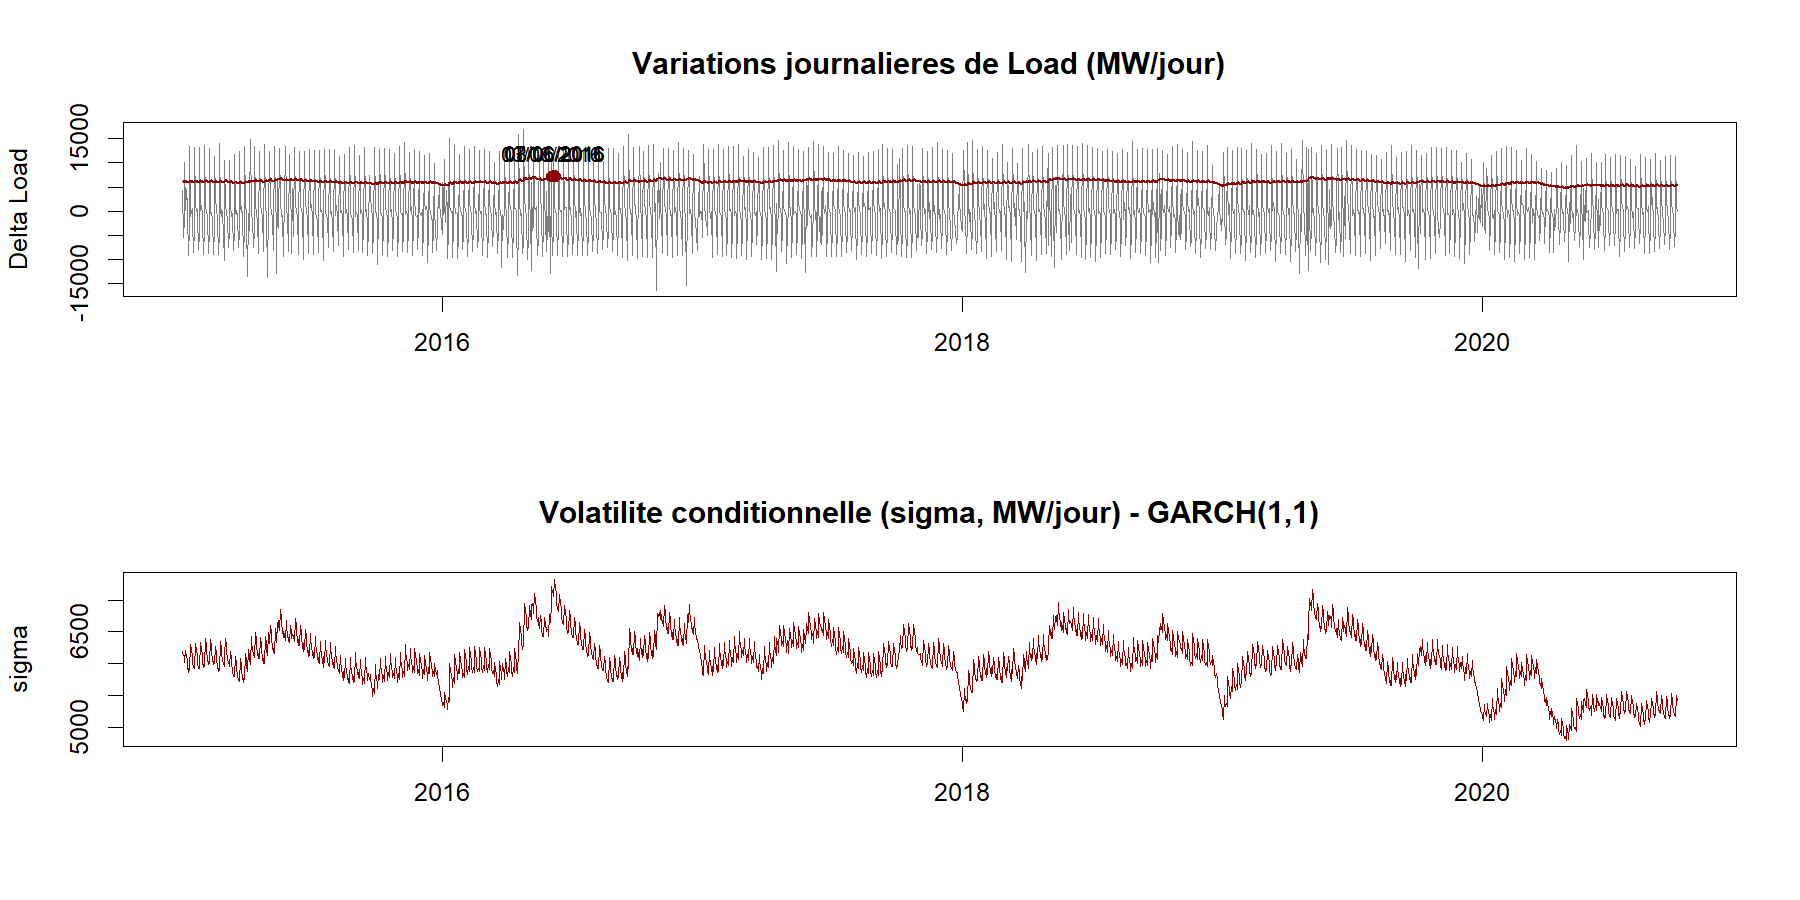
\includegraphics[width=0.9\textwidth]{R_garch_Load.png}
\caption{Volatilité conditionnelle \texttt{Load} (GARCH(1,1), R).}
\label{fig:garch_r_load}
\end{figure}

\begin{figure}[H]
\centering
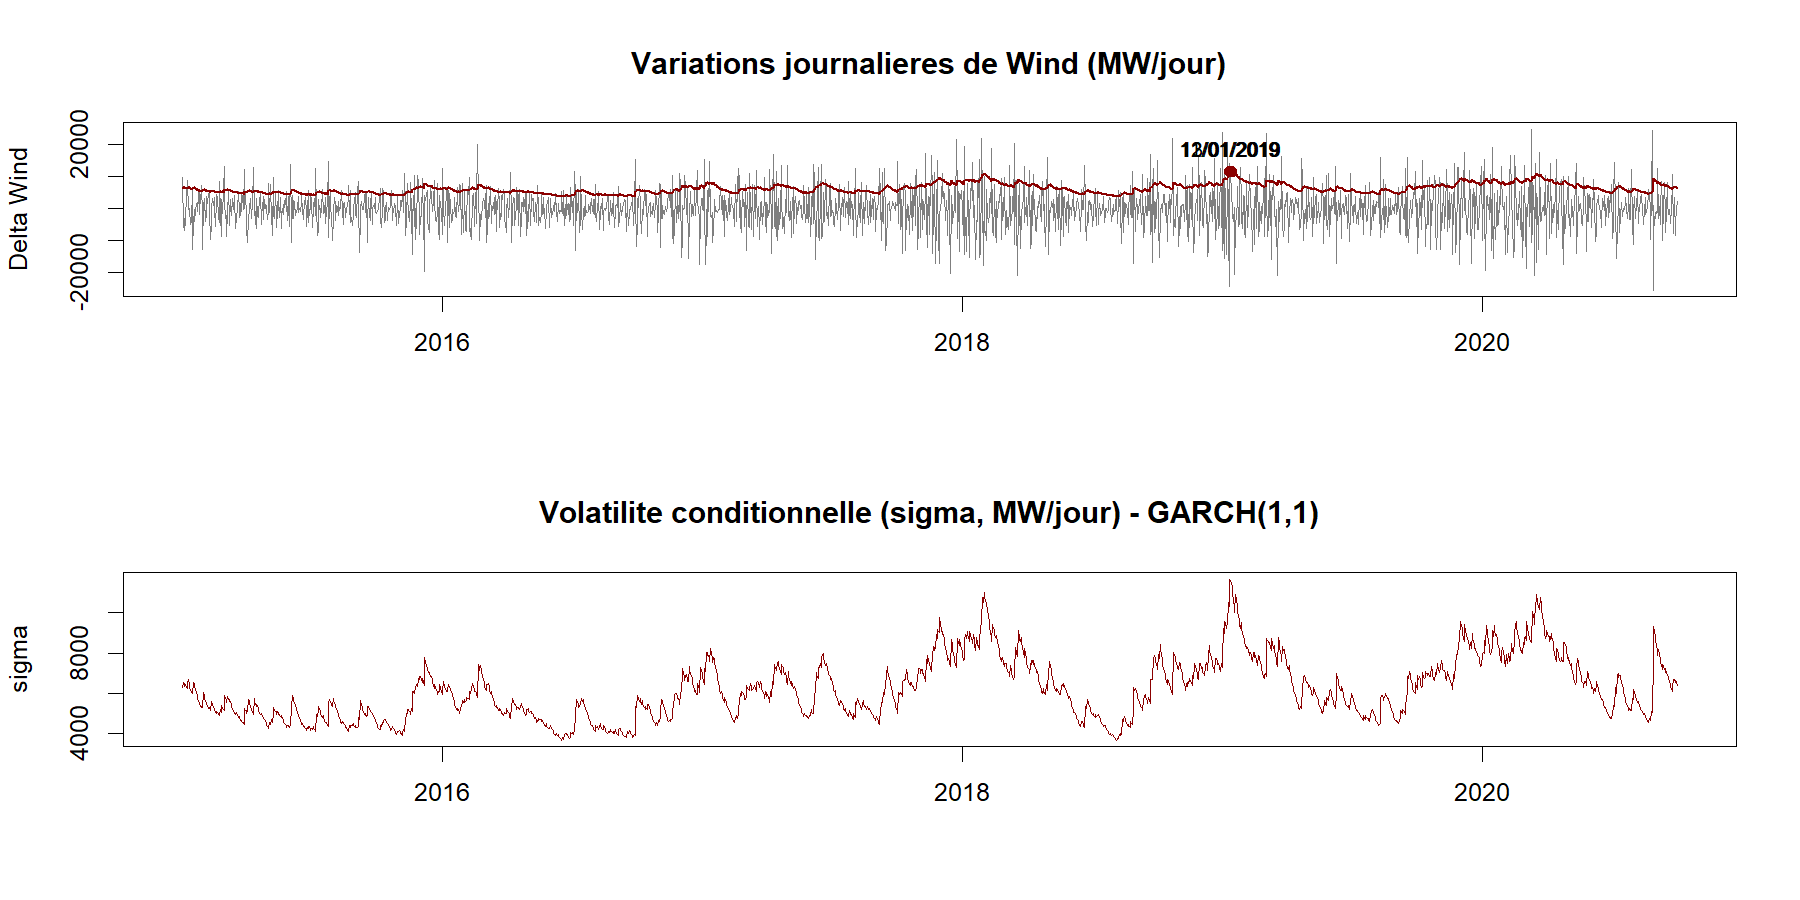
\includegraphics[width=0.9\textwidth]{R_garch_Wind.png}
\caption{Volatilité conditionnelle \texttt{Wind} (GARCH(1,1), R).}
\label{fig:garch_r_wind}
\end{figure}

\begin{figure}[H]
\centering
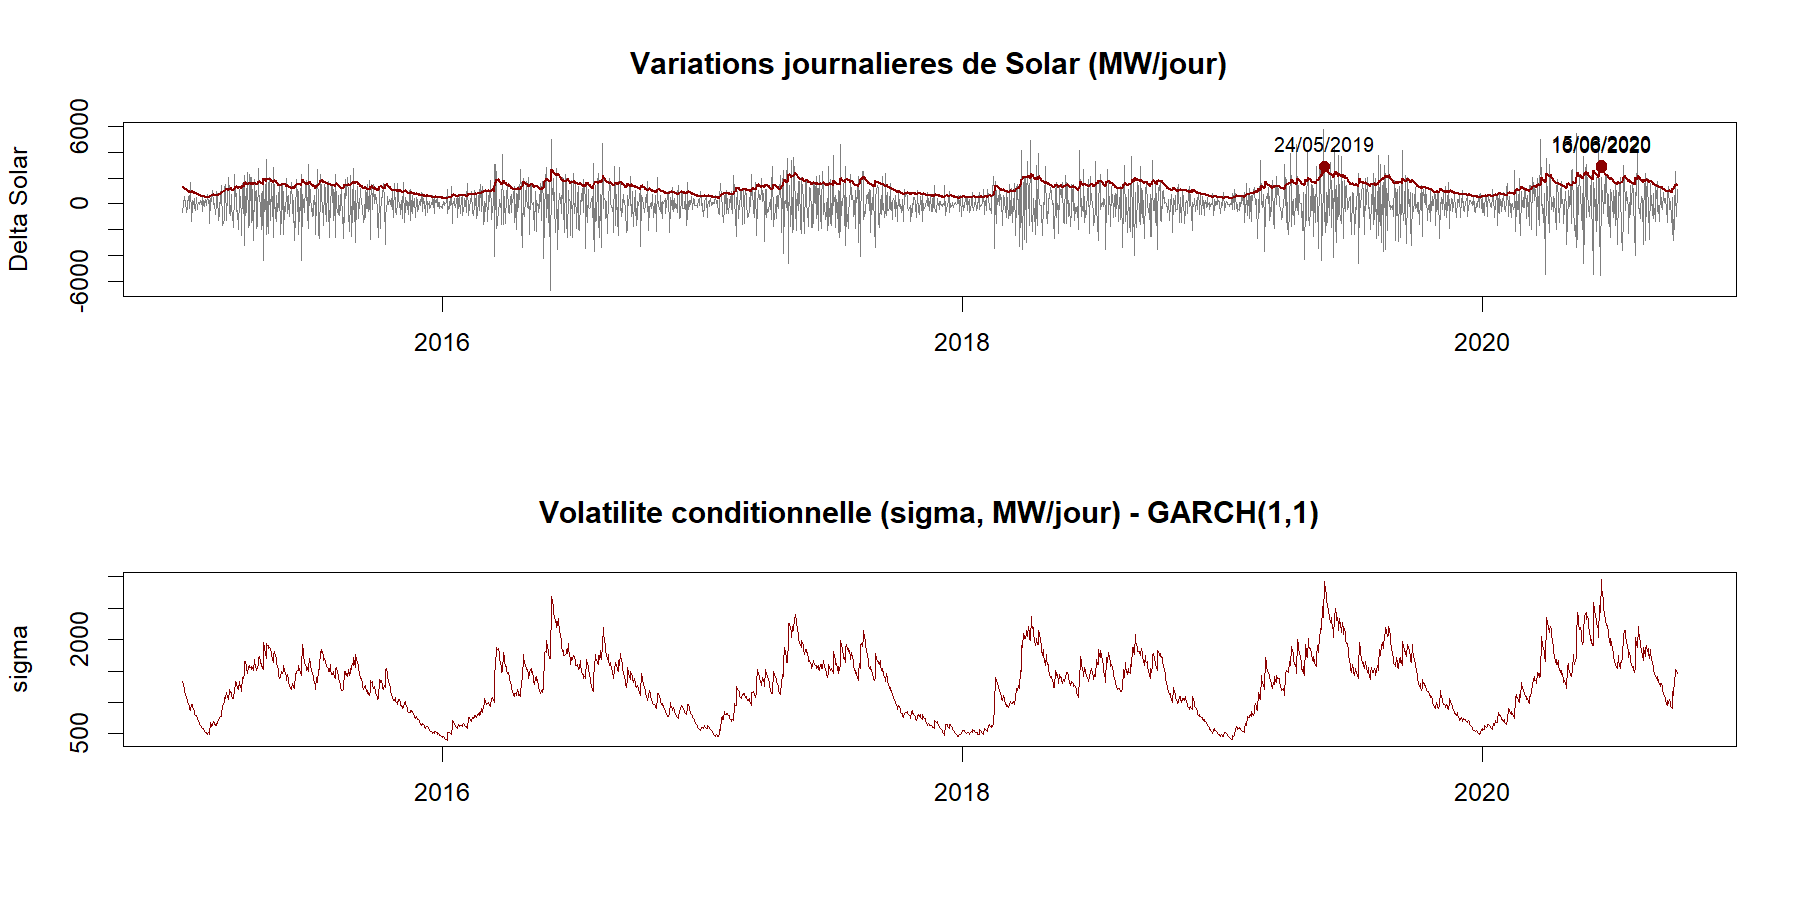
\includegraphics[width=0.9\textwidth]{R_garch_Solar.png}
\caption{Volatilité conditionnelle \texttt{Solar} (GARCH(1,1), R).}
\label{fig:garch_r_solar}
\end{figure}

\begin{figure}[H]
\centering
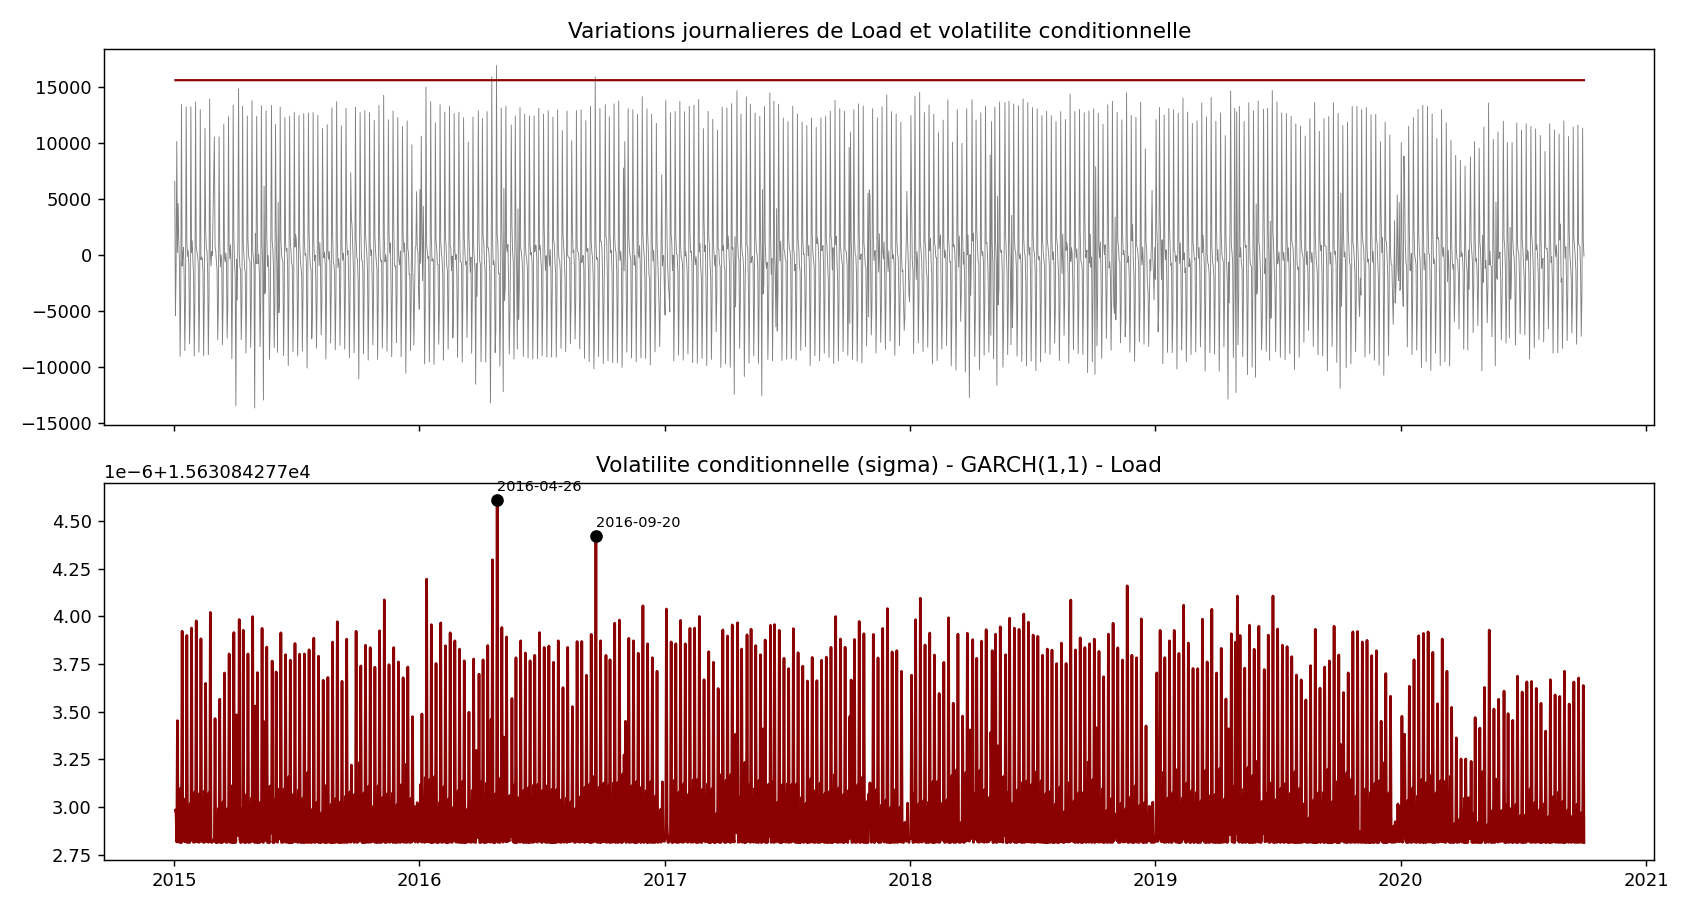
\includegraphics[width=0.9\textwidth]{py_garch_Load.png}
\caption{Volatilité conditionnelle \texttt{Load} (Python).}
\label{fig:garch_py_load}
\end{figure}

\begin{figure}[H]
\centering
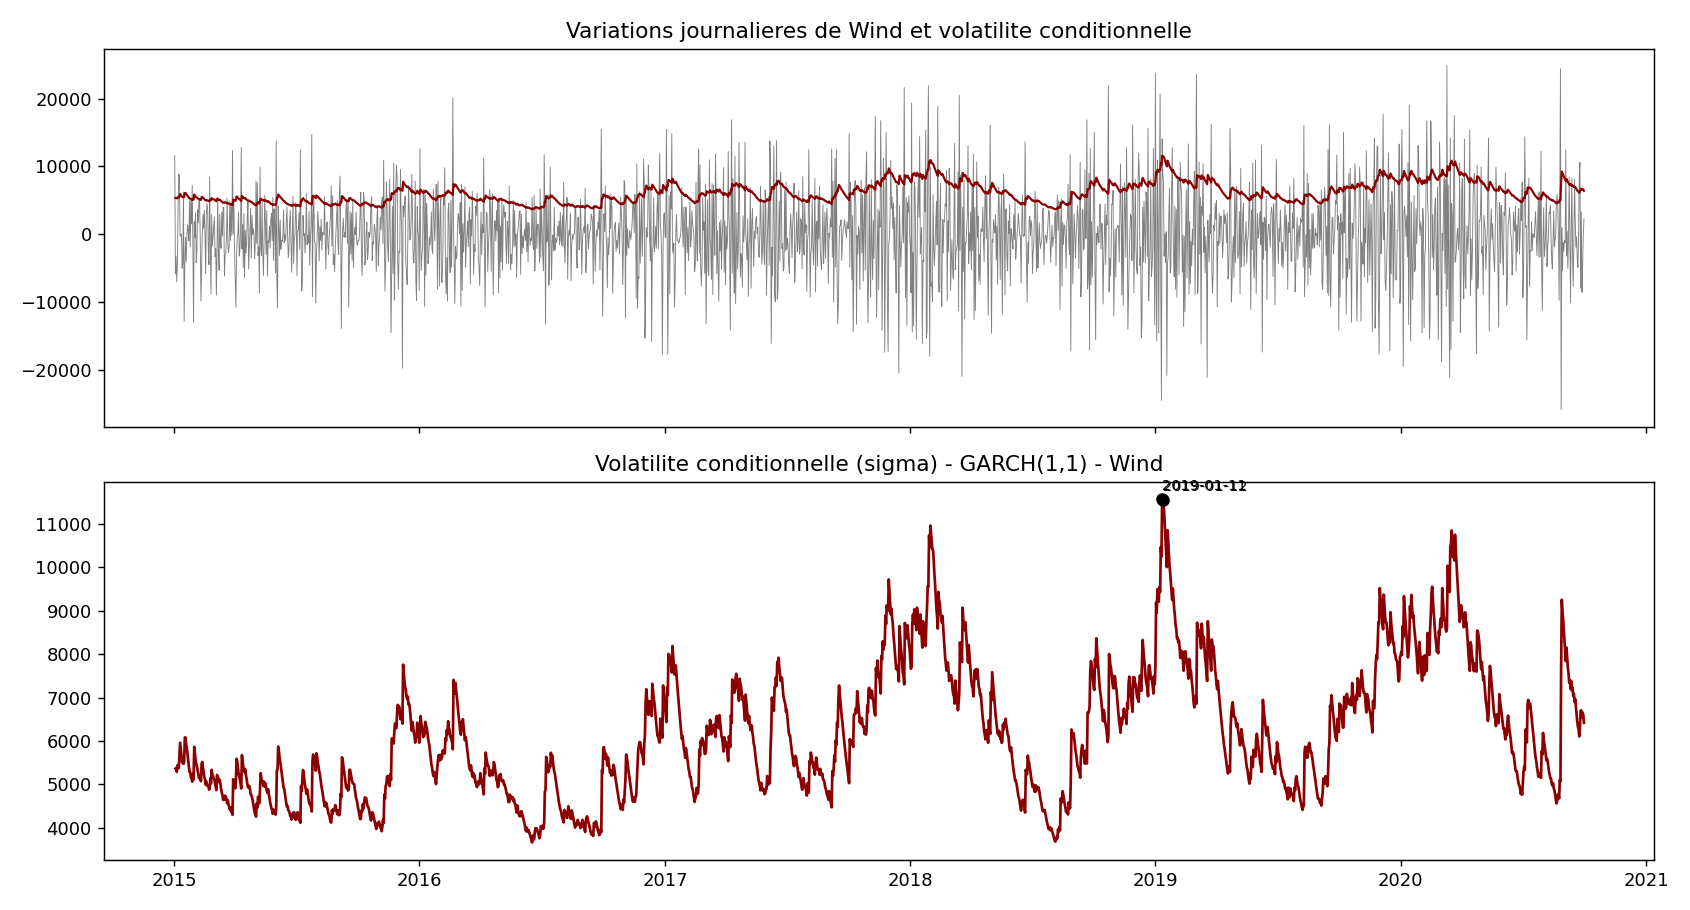
\includegraphics[width=0.9\textwidth]{py_garch_Wind.png}
\caption{Volatilité conditionnelle \texttt{Wind} (Python).}
\label{fig:garch_py_wind}
\end{figure}

\begin{figure}[H]
\centering
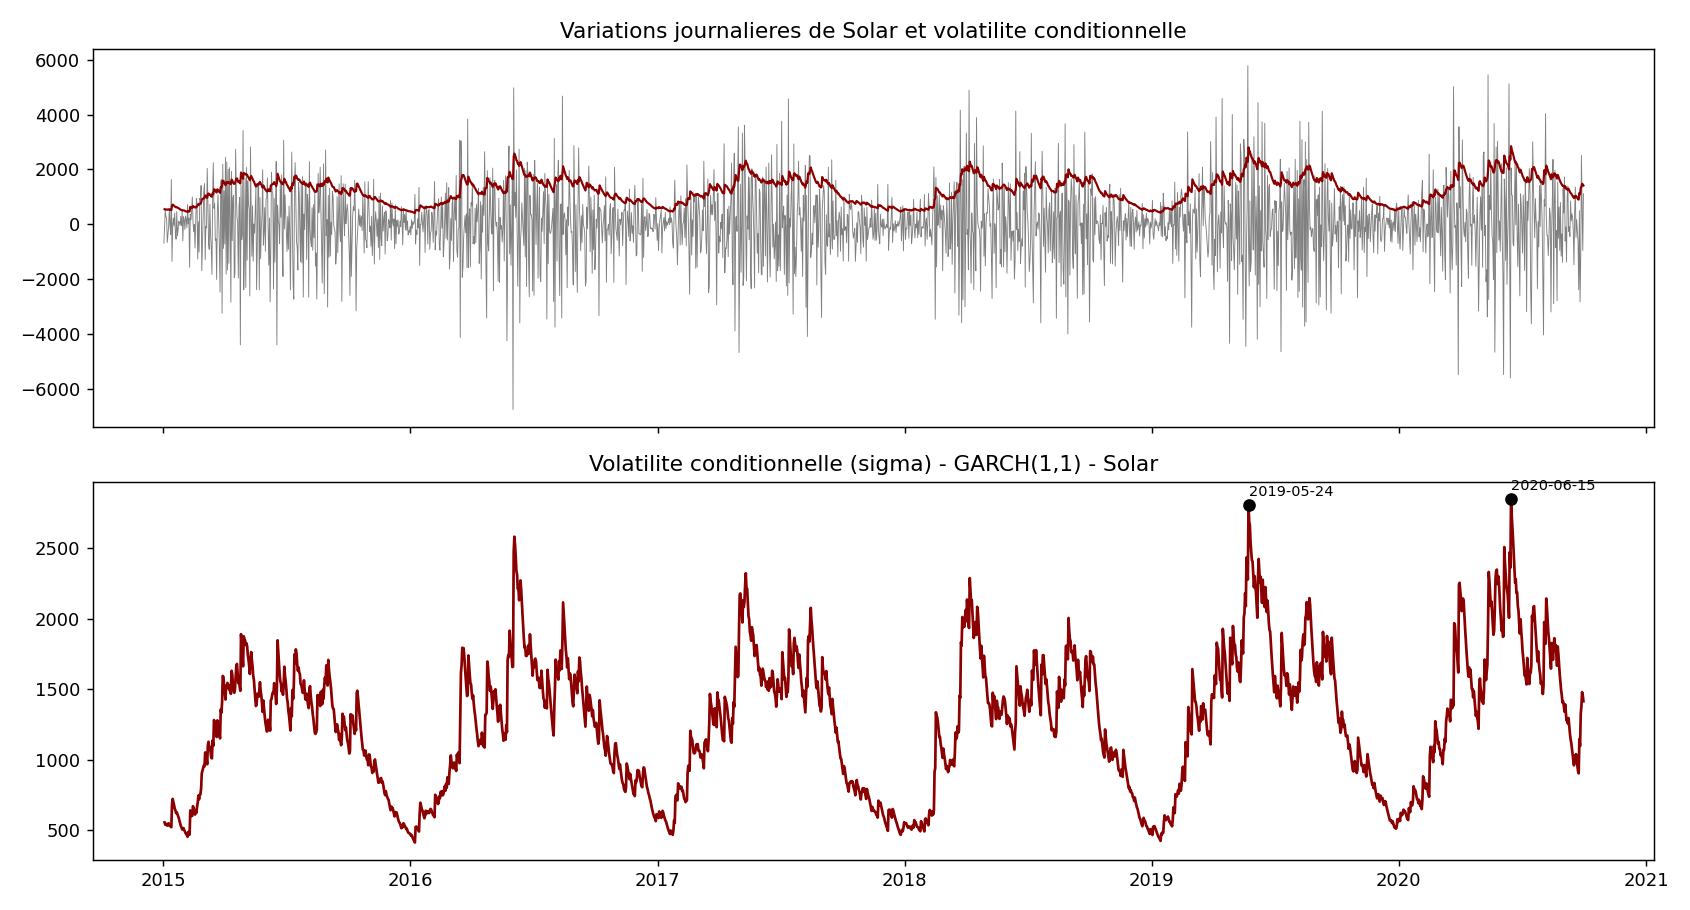
\includegraphics[width=0.9\textwidth]{py_garch_Solar.png}
\caption{Volatilité conditionnelle \texttt{Solar} (Python).}
\label{fig:garch_py_solar}
\end{figure}

\FloatBarrier

\subsection{Modèles profonds : LSTM / GRU}

Deux architectures récurrentes (LSTM et GRU), régularisées par une couche de
\textbf{Dropout} (\(p=0{,}2\)), sont entraînées par série avec une fenêtre
glissante de \(168\)~h et une prévision récursive ; la meilleure architecture
(sur la \texttt{val\_loss}) est conservée. Le tableau~\ref{tab:lstm} présente
les métriques des deux réseaux : la sélection retient le \textbf{LSTM} pour
\texttt{Load} et \texttt{Solar}, le \textbf{GRU} pour \texttt{Wind}. À
\(h=10\), le LSTM atteint une RMSE de \(1\,263{,}0\)~MW sur \texttt{Load}
(\(\text{MAPE}=1{,}57\,\%\)). À \(h=5\,040\), le LSTM reste le plus performant
sur \texttt{Load} (\(7\,592{,}7\)~MW, à comparer aux \(65\,847\)~MW de
SARIMA\_manuel), tandis que le GRU domine sur \texttt{Wind}
(\(8\,567{,}3\)~MW contre \(11\,858{,}4\) pour le LSTM). Sur \texttt{Solar}, le
MAPE devient astronomique (\(\sim 1{,}7\times 10^{14}\,\%\)) : artefact
documenté dû aux valeurs proches de zéro la nuit.

\begin{table}[H]
\centering
\caption{Métriques LSTM/GRU (Python).
Source : \texttt{py\_lstm\_gru\_metrics.csv}.}
\label{tab:lstm}
\small
\begin{tabular}{llrrrr}
\toprule
Variable & Modèle & $h$ & RMSE & MAE & MAPE (\%) \\
\midrule
\texttt{Load}  & LSTM & 10 & 1\,263{,}0 & 967{,}8 & 1{,}57 \\
\texttt{Load}  & LSTM & 24 & 1\,918{,}7 & 1\,555{,}9 & 2{,}44 \\
\texttt{Load}  & LSTM & 5040 & 7\,592{,}7 & 6\,137{,}2 & 13{,}00 \\
\texttt{Load}  & GRU & 10 & 2\,708{,}3 & 2\,259{,}0 & 3{,}60 \\
\texttt{Load}  & GRU & 24 & 8\,406{,}2 & 6\,593{,}0 & 9{,}95 \\
\texttt{Load}  & GRU & 5040 & 9\,033{,}5 & 7\,809{,}0 & 15{,}83 \\
\texttt{Wind}  & LSTM & 10 & 3\,120{,}0 & 2\,819{,}3 & 45{,}38 \\
\texttt{Wind}  & LSTM & 24 & 7\,870{,}1 & 6\,203{,}7 & 42{,}78 \\
\texttt{Wind}  & LSTM & 5040 & 11\,858{,}4 & 10\,584{,}9 & 296{,}93 \\
\texttt{Wind}  & GRU & 10 & 2\,060{,}4 & 1\,847{,}2 & 29{,}89 \\
\texttt{Wind}  & GRU & 24 & 9\,277{,}6 & 6\,759{,}1 & 38{,}99 \\
\texttt{Wind}  & GRU & 5040 & 8\,567{,}3 & 6\,993{,}9 & 172{,}26 \\
\texttt{Solar} & LSTM & 10 & 573{,}8 & 420{,}1 & $5{,}9\text{e}12$ \\
\texttt{Solar} & LSTM & 24 & 579{,}0 & 447{,}7 & $6{,}1\text{e}12$ \\
\texttt{Solar} & LSTM & 5040 & 11\,368{,}4 & 8\,398{,}9 & $1{,}7\text{e}14$ \\
\texttt{Solar} & GRU & 10 & 3\,334{,}2 & 2\,480{,}1 & $6{,}2\text{e}13$ \\
\texttt{Solar} & GRU & 24 & 4\,092{,}7 & 3\,171{,}4 & $8{,}4\text{e}13$ \\
\texttt{Solar} & GRU & 5040 & 10\,534{,}3 & 7\,430{,}5 & $8{,}8\text{e}13$ \\
\bottomrule
\end{tabular}
\end{table}

\paragraph{Validation croisée temporelle (TSCV).}
Une validation croisée à fenêtre expansive (\(k=3\) plis) confirme la
stabilité des réseaux : la RMSE de validation décroît puis se stabilise à
mesure que le train s'allonge (\texttt{Load}\,: \(2\,178\to1\,907\)~MW pour le
LSTM ; \texttt{Wind}\,: \(957\to876\)~MW pour le GRU ; \texttt{Solar}\,:
\(1\,422\to1\,146\)~MW pour le LSTM). Source :
\texttt{py\_lstm\_gru\_cv.csv}.

Les figures~\ref{fig:lstm_forecast_load}--\ref{fig:lstm_forecast_solar}
comparent prévisions et valeurs réelles, et les figures de \emph{loss}
(\ref{fig:lstm_loss_load}--\ref{fig:lstm_loss_solar}) illustrent la
convergence de l'apprentissage (train/validation).

\begin{figure}[H]
\centering
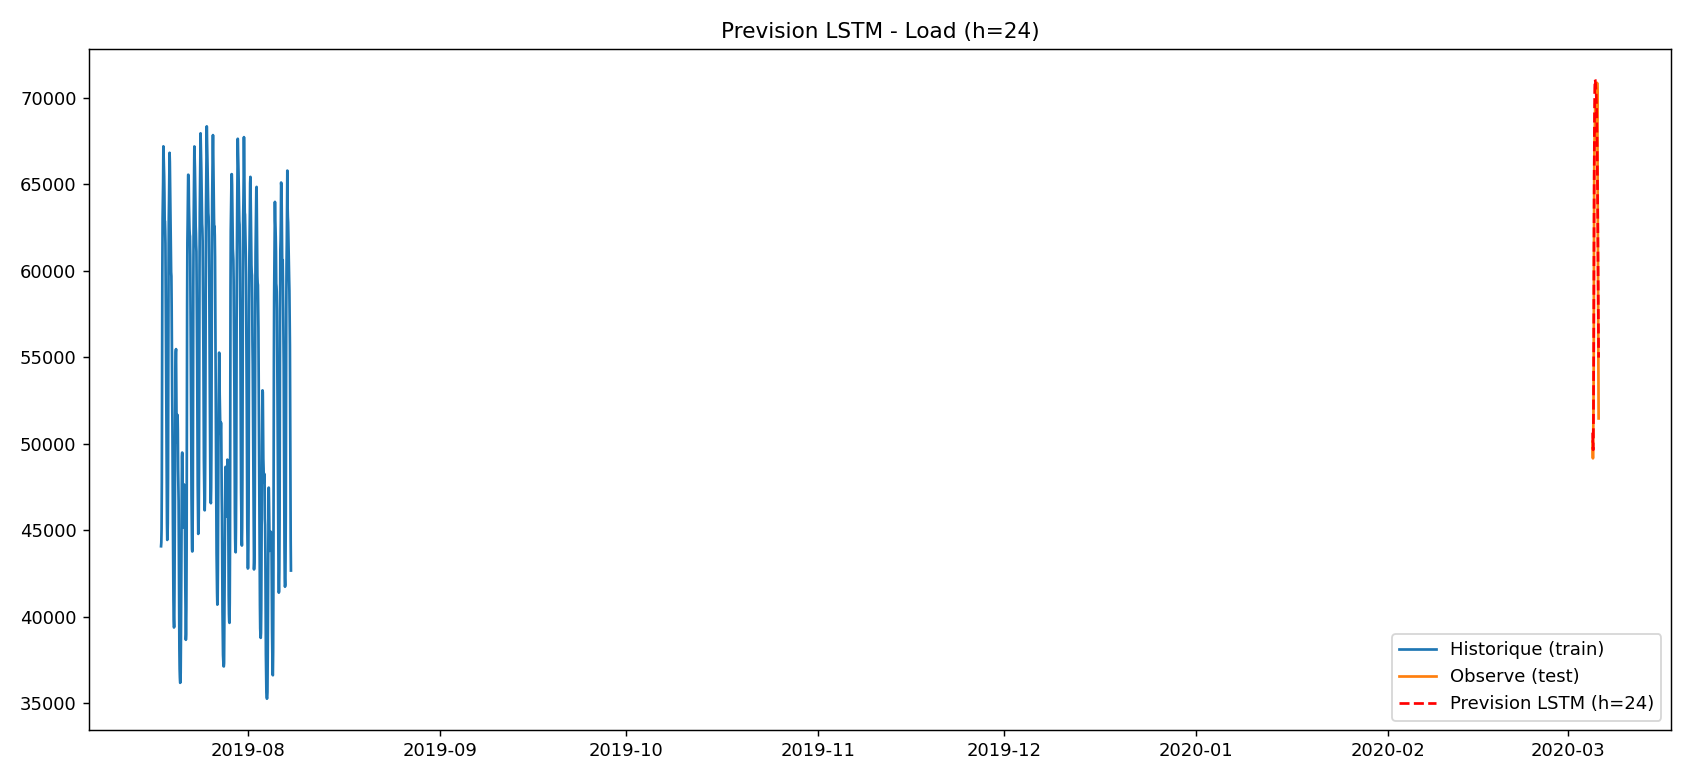
\includegraphics[width=0.9\textwidth]{py_lstm_gru_forecast_Load.png}
\caption{Prévisions LSTM/GRU -- \texttt{Load}.}
\label{fig:lstm_forecast_load}
\end{figure}

\begin{figure}[H]
\centering
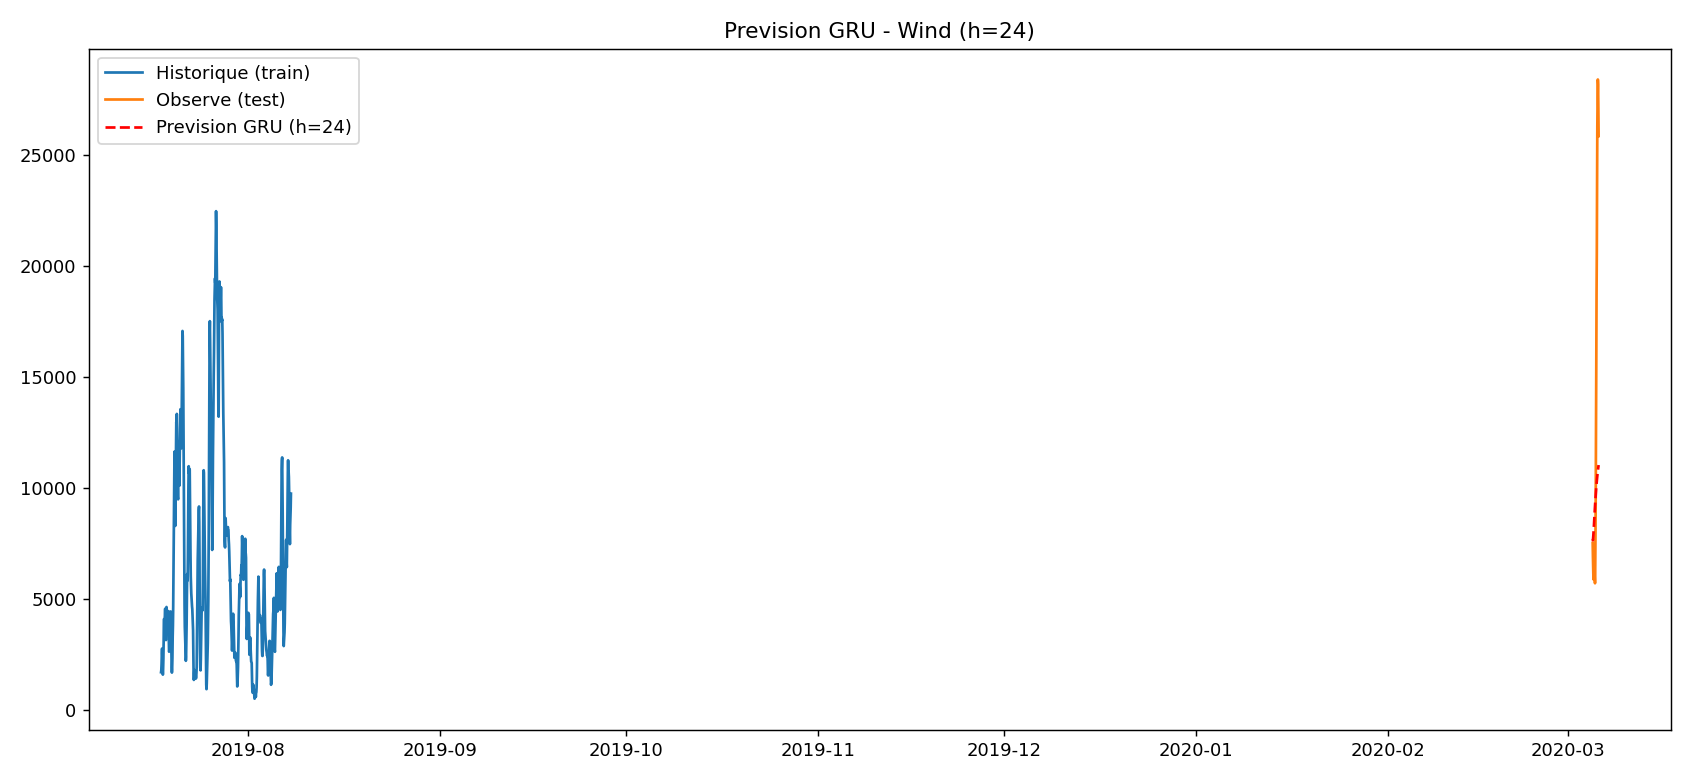
\includegraphics[width=0.9\textwidth]{py_lstm_gru_forecast_Wind.png}
\caption{Prévisions LSTM/GRU -- \texttt{Wind}.}
\label{fig:lstm_forecast_wind}
\end{figure}

\begin{figure}[H]
\centering
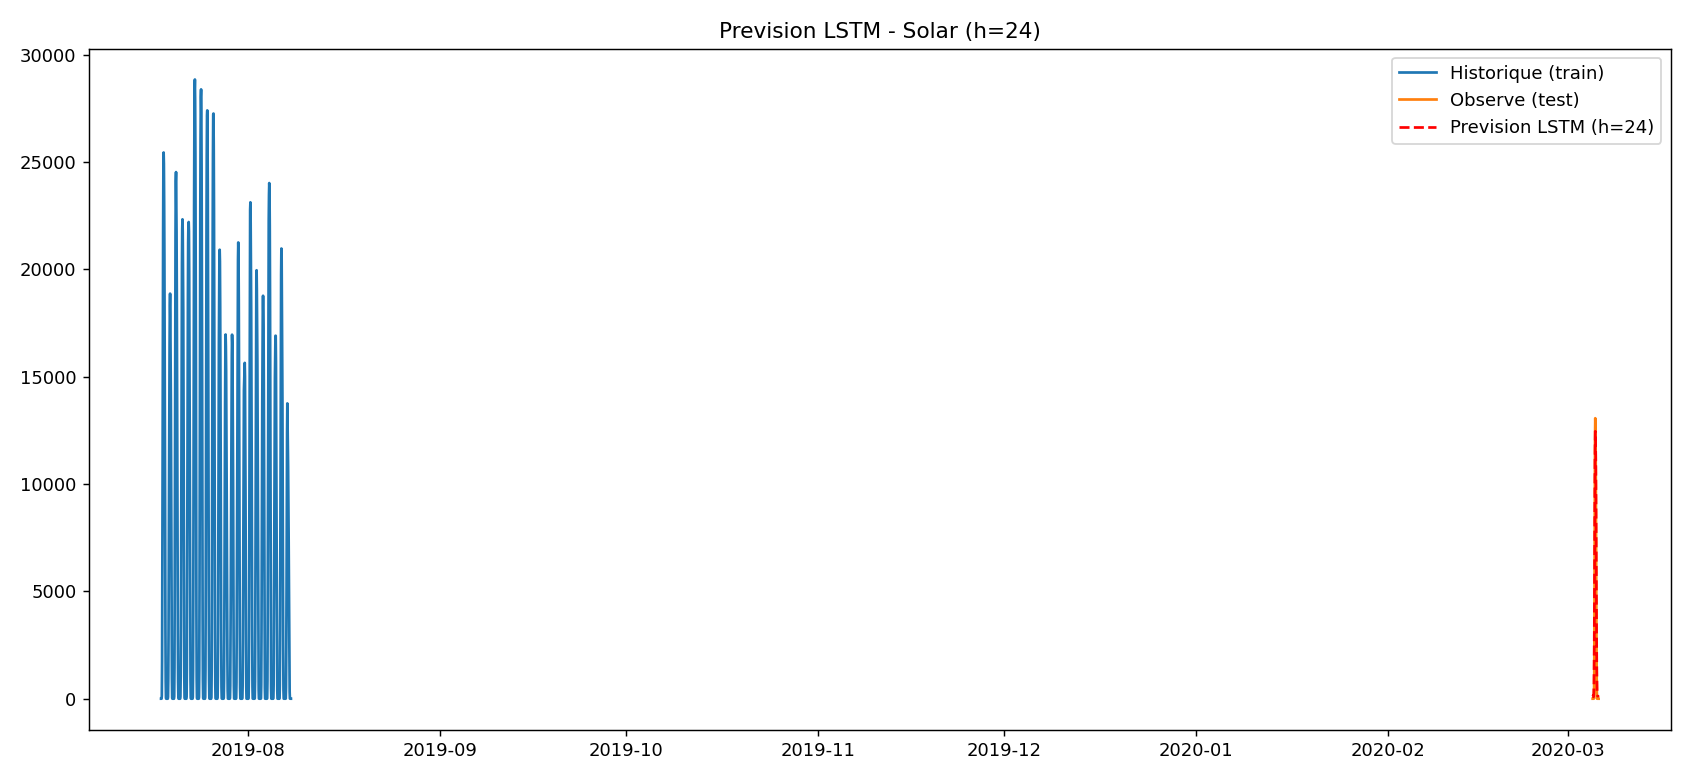
\includegraphics[width=0.9\textwidth]{py_lstm_gru_forecast_Solar.png}
\caption{Prévisions LSTM/GRU -- \texttt{Solar}.}
\label{fig:lstm_forecast_solar}
\end{figure}

\begin{figure}[H]
\centering
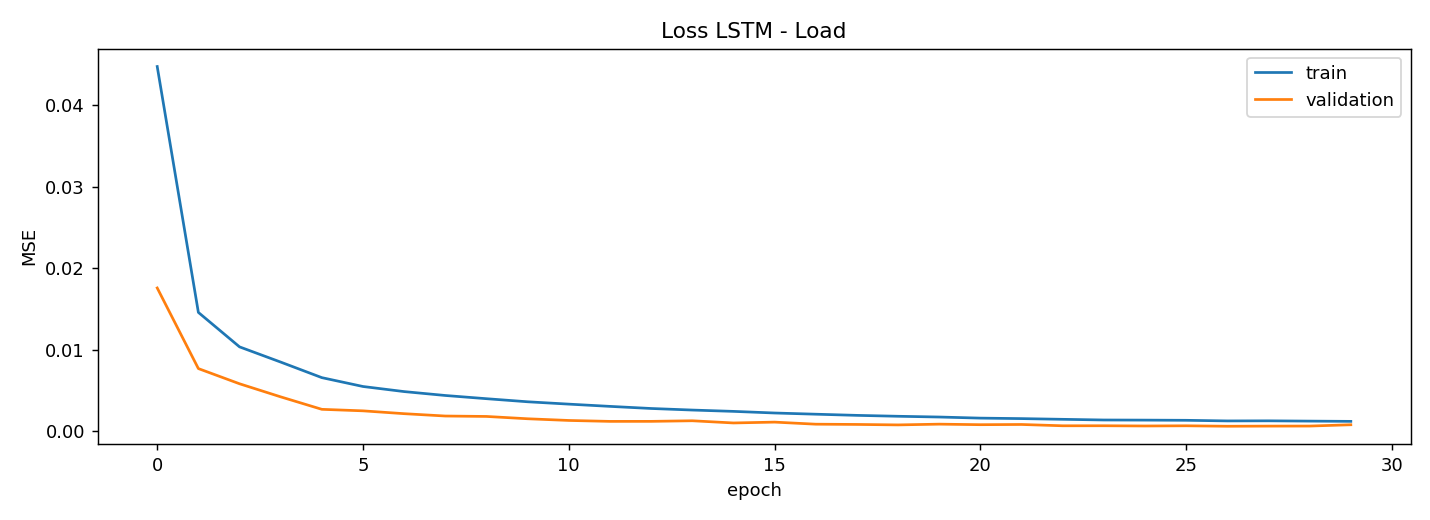
\includegraphics[width=0.75\textwidth]{py_lstm_gru_loss_Load.png}
\caption{Courbes de \emph{loss} -- \texttt{Load}.}
\label{fig:lstm_loss_load}
\end{figure}

\begin{figure}[H]
\centering
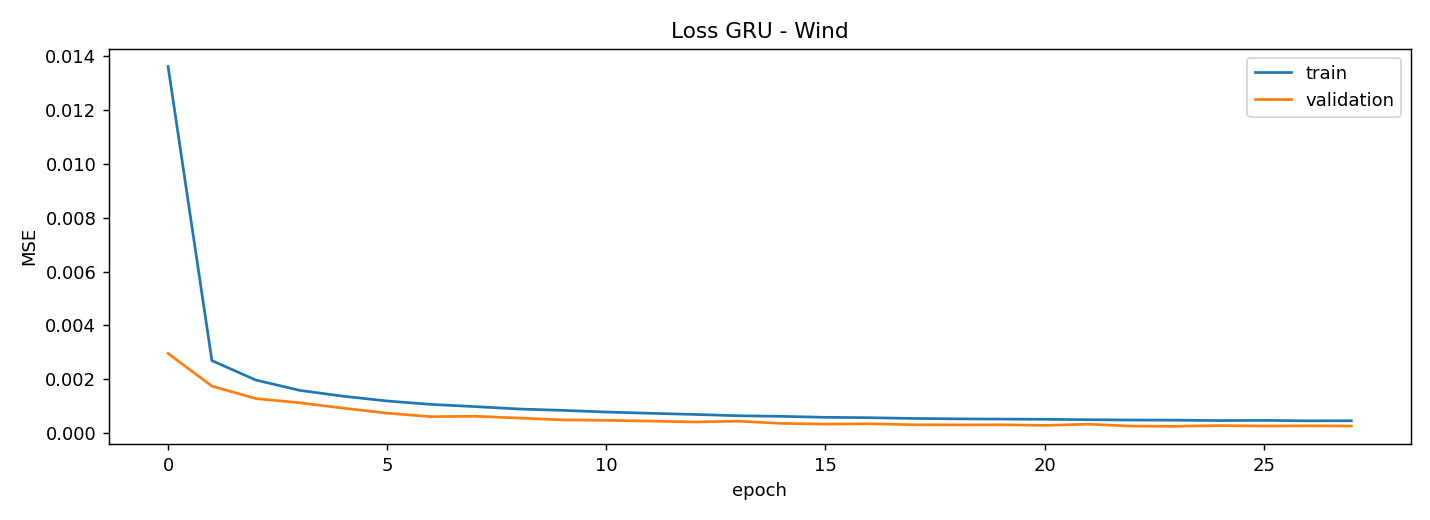
\includegraphics[width=0.75\textwidth]{py_lstm_gru_loss_Wind.png}
\caption{Courbes de \emph{loss} -- \texttt{Wind}.}
\label{fig:lstm_loss_wind}
\end{figure}

\begin{figure}[H]
\centering
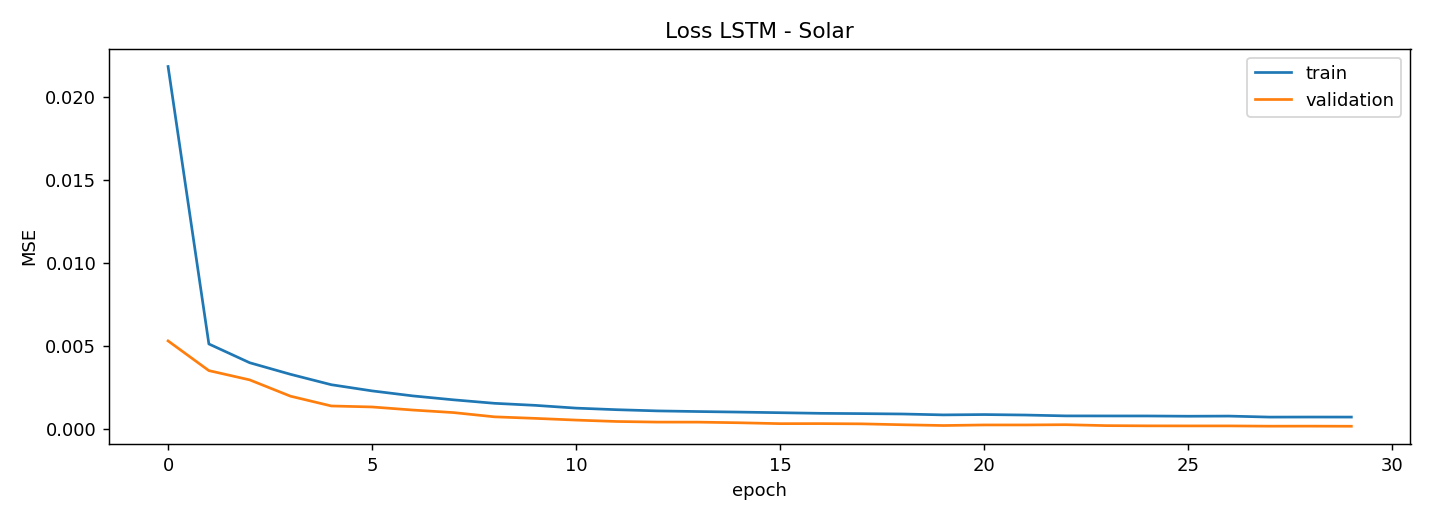
\includegraphics[width=0.75\textwidth]{py_lstm_gru_loss_Solar.png}
\caption{Courbes de \emph{loss} -- \texttt{Solar}.}
\label{fig:lstm_loss_solar}
\end{figure}

\FloatBarrier

\section{Évaluation comparative}
\label{sec:evaluation}

\subsection{Classement général (R vs Python vs LSTM/GRU)}
Le classement agrégé \texttt{py\_evaluation\_ranking.csv} confronte, pour
chaque couple (Variable, Horizon), les modèles R classiques, Python classiques
et LSTM/GRU selon RMSE/MAE/MAPE. Le tableau~\ref{tab:ranking_top} en extrait
les meilleurs modèles par variable et par horizon.

\begin{table}[H]
\centering
\caption{Meilleurs modèles par variable et par horizon (extrait de
\texttt{py\_evaluation\_ranking.csv}).}
\label{tab:ranking_top}
\small
\begin{tabular}{lllrr}
\toprule
Variable & $h$ & Meilleur modèle (RMSE le plus faible) & RMSE & MAPE (\%) \\
\midrule
\texttt{Load}  & 10   & Hybride\_SARIMA\_LSTM (Python) & 780{,}6 & 1{,}20 \\
\texttt{Load}  & 24   & Hybride\_SARIMA\_LSTM (Python) & 970{,}7 & 1{,}35 \\
\texttt{Load}  & 5040 & Prophet (Python)              & 3\,985{,}9 & 6{,}33 \\
\texttt{Wind}  & 10   & ARIMA\_auto (R)               & 512{,}4  & 7{,}37 \\
\texttt{Wind}  & 24   & LSTM (Python)                 & 7\,870{,}1 & 42{,}78 \\
\texttt{Wind}  & 5040 & GRU (Python)                  & 8\,567{,}3 & 172{,}26 \\
\texttt{Solar} & 10   & Hybride\_SARIMA\_LSTM (Python) & 528{,}0  & 282{,}44 \\
\texttt{Solar} & 24   & LSTM (Python)                 & 579{,}0  & 6{,}07e12 \\
\texttt{Solar} & 5040 & Prophet (Python)              & 5\,020{,}4 & 8\,127{,}28 \\
\bottomrule
\end{tabular}
\end{table}

La figure~\ref{fig:eval_rmse} synthétise ces RMSE. Les enseignements sont :
\begin{itemize}
  \item à \textbf{court terme} (\(h=10\)), un modèle \textbf{hybride
        SARIMA$\,$+$\,$LSTM} (Python) obtient la meilleure RMSE sur
        \texttt{Load} et \texttt{Solar} ; la transposition classique
        (\texttt{SARIMA\_manuel}) reste très proche, avec des résultats
        \textbf{quasi identiques} en R et en Python (reproductibilité
        confirmée) ;
  \item à \textbf{l'horizon journalier} (\(h=24\)), les modèles profonds
        (LSTM) prennent l'avantage sur \texttt{Wind} et \texttt{Solar}, tandis
        que l'hybride conserve la première place sur \texttt{Load} ;
  \item à \textbf{très long terme} (\(h=5\,040\)), \textbf{Prophet} domine sur
        \texttt{Load} (RMSE divisée par \(4\) par rapport au LSTM) et
        \texttt{Solar}, et les réseaux récurrents (\textbf{GRU} pour la RMSE)
        s'imposent sur \texttt{Wind} ;
  \item \texttt{Solar} reste la série la plus difficile, en raison de sa
        nature intermittente, de ses valeurs nulles (MAPE ininterprétable) et
        du test débutant pendant la période COVID-19.
\end{itemize}

\begin{figure}[H]
\centering
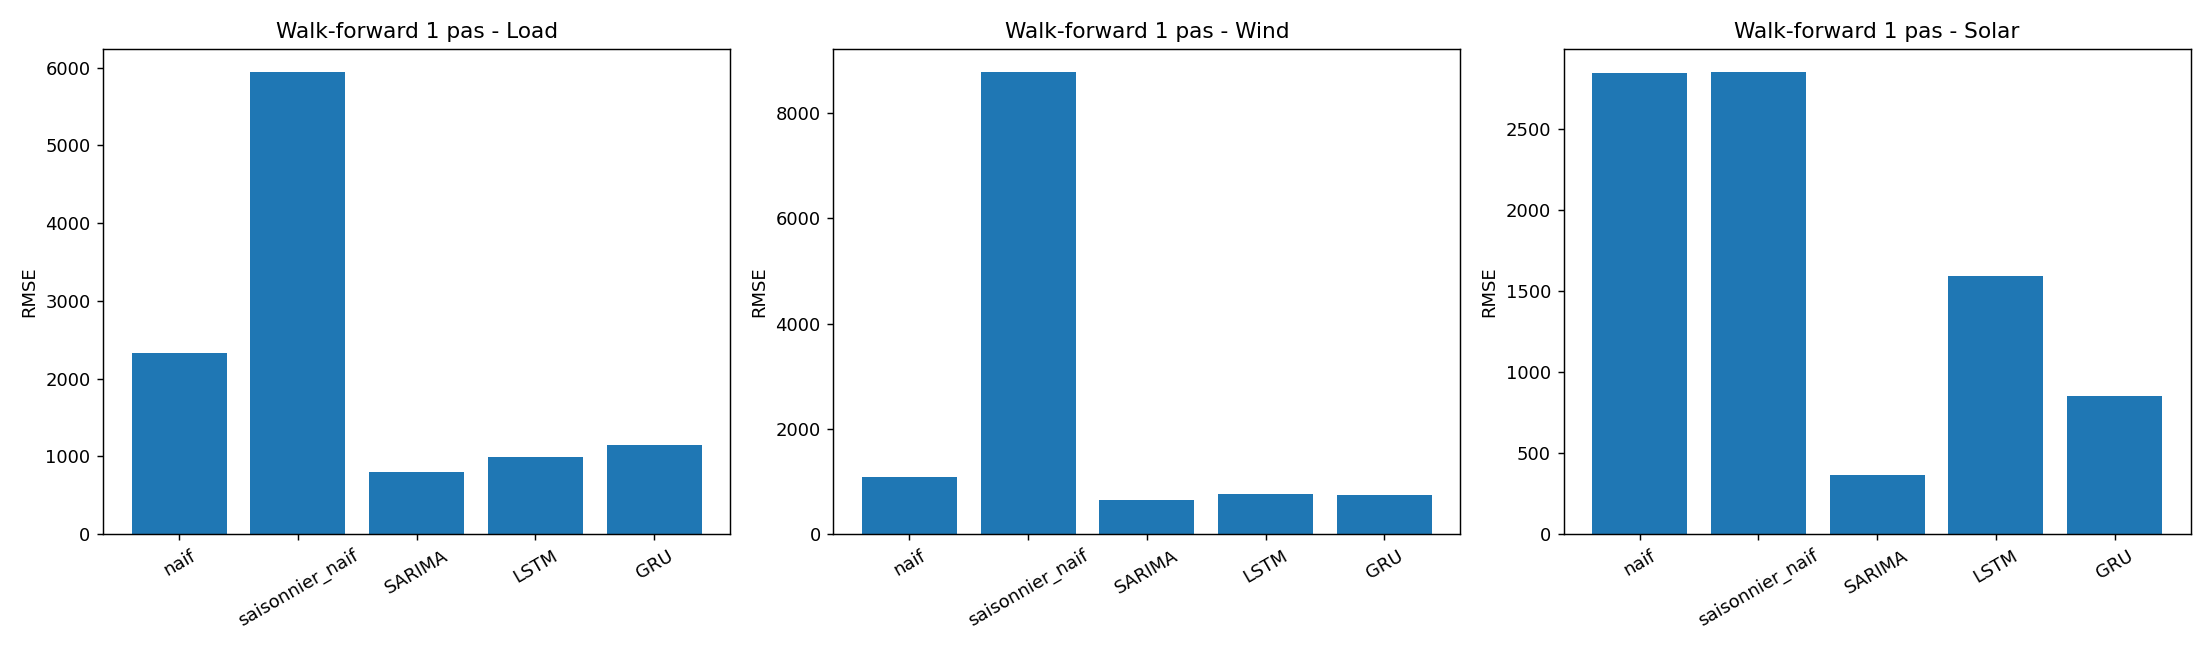
\includegraphics[width=0.95\textwidth]{py_evaluation_rmse.png}
\caption{Comparaison des RMSE par variable et par horizon.}
\label{fig:eval_rmse}
\end{figure}

\subsection{Walk-forward à un pas}
L'évaluation walk-forward à un pas confronte les baselines \emph{naïve} et
\emph{saisonnière-naïve} (\(24\)~h) au SARIMA retenu, au LSTM et au GRU, sur
les \(5\,040\)~h du test. Le tableau~\ref{tab:walkforward} montre que le
\textbf{SARIMA} obtient les meilleures métriques pour les trois séries
(\texttt{Load}\,: RMSE \(797{,}1\) contre \(998{,}3\) pour le LSTM ;
\texttt{Solar}\,: \(367{,}0\) contre \(856{,}0\) pour le GRU). Les réseaux
récurrents restent néanmoins nettement supérieurs aux modèles naïfs. Les
prévisions sont archivées dans \texttt{results/forecasts/py\_walkforward\_*.csv}.

\begin{table}[H]
\centering
\caption{Métriques walk-forward à un pas.
Source : \texttt{py\_walkforward\_metrics.csv}.}
\label{tab:walkforward}
\small
\begin{tabular}{llrrr}
\toprule
Variable & Modèle & MSE & RMSE & MAE \\
\midrule
\texttt{Load}  & naïf             & 5\,420\,103 & 2\,328{,}1 & 1\,807{,}0 \\
\texttt{Load}  & saisonnier naïf  & 35\,376\,448 & 5\,947{,}8 & 3\,889{,}6 \\
\texttt{Load}  & SARIMA           & 635\,357 & 797{,}1 & 590{,}3 \\
\texttt{Load}  & LSTM             & 996\,585 & 998{,}3 & 771{,}7 \\
\texttt{Load}  & GRU              & 1\,307\,527 & 1\,143{,}5 & 875{,}7 \\
\texttt{Wind}  & naïf             & 1\,187\,705 & 1\,089{,}8 & 782{,}6 \\
\texttt{Wind}  & saisonnier naïf  & 77\,192\,711 & 8\,785{,}9 & 6\,358{,}1 \\
\texttt{Wind}  & SARIMA           & 427\,719 & 654{,}0 & 452{,}9 \\
\texttt{Wind}  & LSTM             & 577\,189 & 759{,}7 & 552{,}9 \\
\texttt{Wind}  & GRU              & 544\,219 & 737{,}7 & 520{,}4 \\
\texttt{Solar} & naïf             & 8\,114\,702 & 2\,848{,}6 & 1\,889{,}3 \\
\texttt{Solar} & saisonnier naïf  & 8\,153\,433 & 2\,855{,}4 & 1\,417{,}7 \\
\texttt{Solar} & SARIMA           & 134\,710 & 367{,}0 & 245{,}0 \\
\texttt{Solar} & LSTM             & 2\,549\,469 & 1\,596{,}7 & 1\,344{,}4 \\
\texttt{Solar} & GRU              & 732\,792 & 856{,}0 & 659{,}0 \\
\bottomrule
\end{tabular}
\end{table}

\subsection{Test de Diebold--Mariano}
Le test de Diebold--Mariano est appliqué à \textbf{toutes les paires} de
modèles du walk-forward sur les erreurs quadratiques (un pas), avec
correction HLN et variance HAC (retard 1). Le tableau~\ref{tab:dm} en
présente les comparaisons clés. Toutes les statistiques sont hautement
significatives (\(p\)-valeurs \(<10^{-18}\) dans l'écrasante majorité des
cas) : sans ambiguïté, le \textbf{SARIMA est statistiquement meilleur} que
les naïfs, le LSTM et le GRU pour les trois séries. Entre réseaux, le
\textbf{LSTM} l'emporte sur \texttt{Load} et le \textbf{GRU} sur
\texttt{Wind} et \texttt{Solar}.

\begin{table}[H]
\centering
\caption{Test de Diebold--Mariano (extrait des paires du walk-forward).
Source : \texttt{py\_diebold\_mariano.csv}.}
\label{tab:dm}
\small
\begin{tabular}{llrrl}
\toprule
Variable & A vs B & DM stat & $p$-valeur & Conclusion \\
\midrule
\texttt{Load}  & naïf vs SARIMA            & $+38{,}62$ & $4{,}37\text{e-}286$ & SARIMA meilleur \\
\texttt{Load}  & saisonnier naïf vs SARIMA & $+34{,}60$ & $1{,}56\text{e-}235$ & SARIMA meilleur \\
\texttt{Load}  & SARIMA vs LSTM            & $-16{,}19$ & $1{,}65\text{e-}57$  & SARIMA meilleur \\
\texttt{Load}  & SARIMA vs GRU             & $-24{,}11$ & $1{,}25\text{e-}121$ & SARIMA meilleur \\
\texttt{Load}  & LSTM vs GRU               & $-12{,}07$ & $4{,}17\text{e-}33$  & LSTM meilleur \\
\texttt{Wind}  & naïf vs SARIMA            & $25{,}44$  & $2{,}01\text{e-}134$ & SARIMA meilleur \\
\texttt{Wind}  & saisonnier naïf vs SARIMA & $35{,}92$  & $9{,}97\text{e-}252$ & SARIMA meilleur \\
\texttt{Wind}  & SARIMA vs LSTM            & $-14{,}63$ & $1{,}69\text{e-}47$  & SARIMA meilleur \\
\texttt{Wind}  & SARIMA vs GRU             & $-11{,}26$ & $4{,}85\text{e-}29$  & SARIMA meilleur \\
\texttt{Wind}  & LSTM vs GRU               & $8{,}87$   & $1{,}03\text{e-}18$  & GRU meilleur \\
\texttt{Solar} & naïf vs SARIMA            & $44{,}27$  & $0{,}00$             & SARIMA meilleur \\
\texttt{Solar} & saisonnier naïf vs SARIMA & $21{,}60$  & $5{,}05\text{e-}99$  & SARIMA meilleur \\
\texttt{Solar} & SARIMA vs LSTM            & $-63{,}20$ & $0{,}00$             & SARIMA meilleur \\
\texttt{Solar} & SARIMA vs GRU             & $-31{,}18$ & $2{,}55\text{e-}195$ & SARIMA meilleur \\
\texttt{Solar} & LSTM vs GRU               & $39{,}75$  & $9{,}23\text{e-}301$ & GRU meilleur \\
\bottomrule
\end{tabular}
\end{table}

\paragraph{Nuance importante.}
Ce résultat concerne la prévision \textbf{à un pas} (walk-forward). Il met en
évidence la supériorité du SARIMA à un pas (filtre de Kalman mis à jour),
qui ne contredit pas l'avantage des modèles profonds sur les \emph{trajectoires
récursives} multi-pas (cf. tableau~\ref{tab:lstm}), ni l'explosion du MAPE
pour \texttt{Solar}. Le test DM entre SARIMA et LSTM sur les trajectoires
\(h>1\) constitue une piste d'approfondissement
(cf. section~\ref{sec:conclusion}).

\section{Interface interactive : dashboard Streamlit}
\label{sec:dashboard}

Afin de restituer les résultats de façon exploratoire, un \emph{dashboard}
\textbf{Streamlit} a été développé (dossier \texttt{dashboard/}). Il se lance
par la commande :
\begin{center}
\texttt{streamlit run dashboard/app.py}
\end{center}
et lit directement les sorties des scripts R/Python
(\texttt{results/figures/}, \texttt{results/tables/} et
\texttt{results/forecasts/}). Il est composé d'une page d'accueil et de cinq
pages accessibles via la barre latérale. Les captures d'écran ci-dessous
(documentées dans \texttt{results/dashboard/}) illustrent chaque interface.

\subsection{Vue d'ensemble}
La page d'accueil affiche des indicateurs synthétiques (nombre de figures, de
tableaux et de prévisions) et le \emph{Top 8} des meilleurs RMSE par couple
(Variable, Horizon), extrait de \texttt{py\_evaluation\_ranking.csv}.

\begin{figure}[H]
\centering
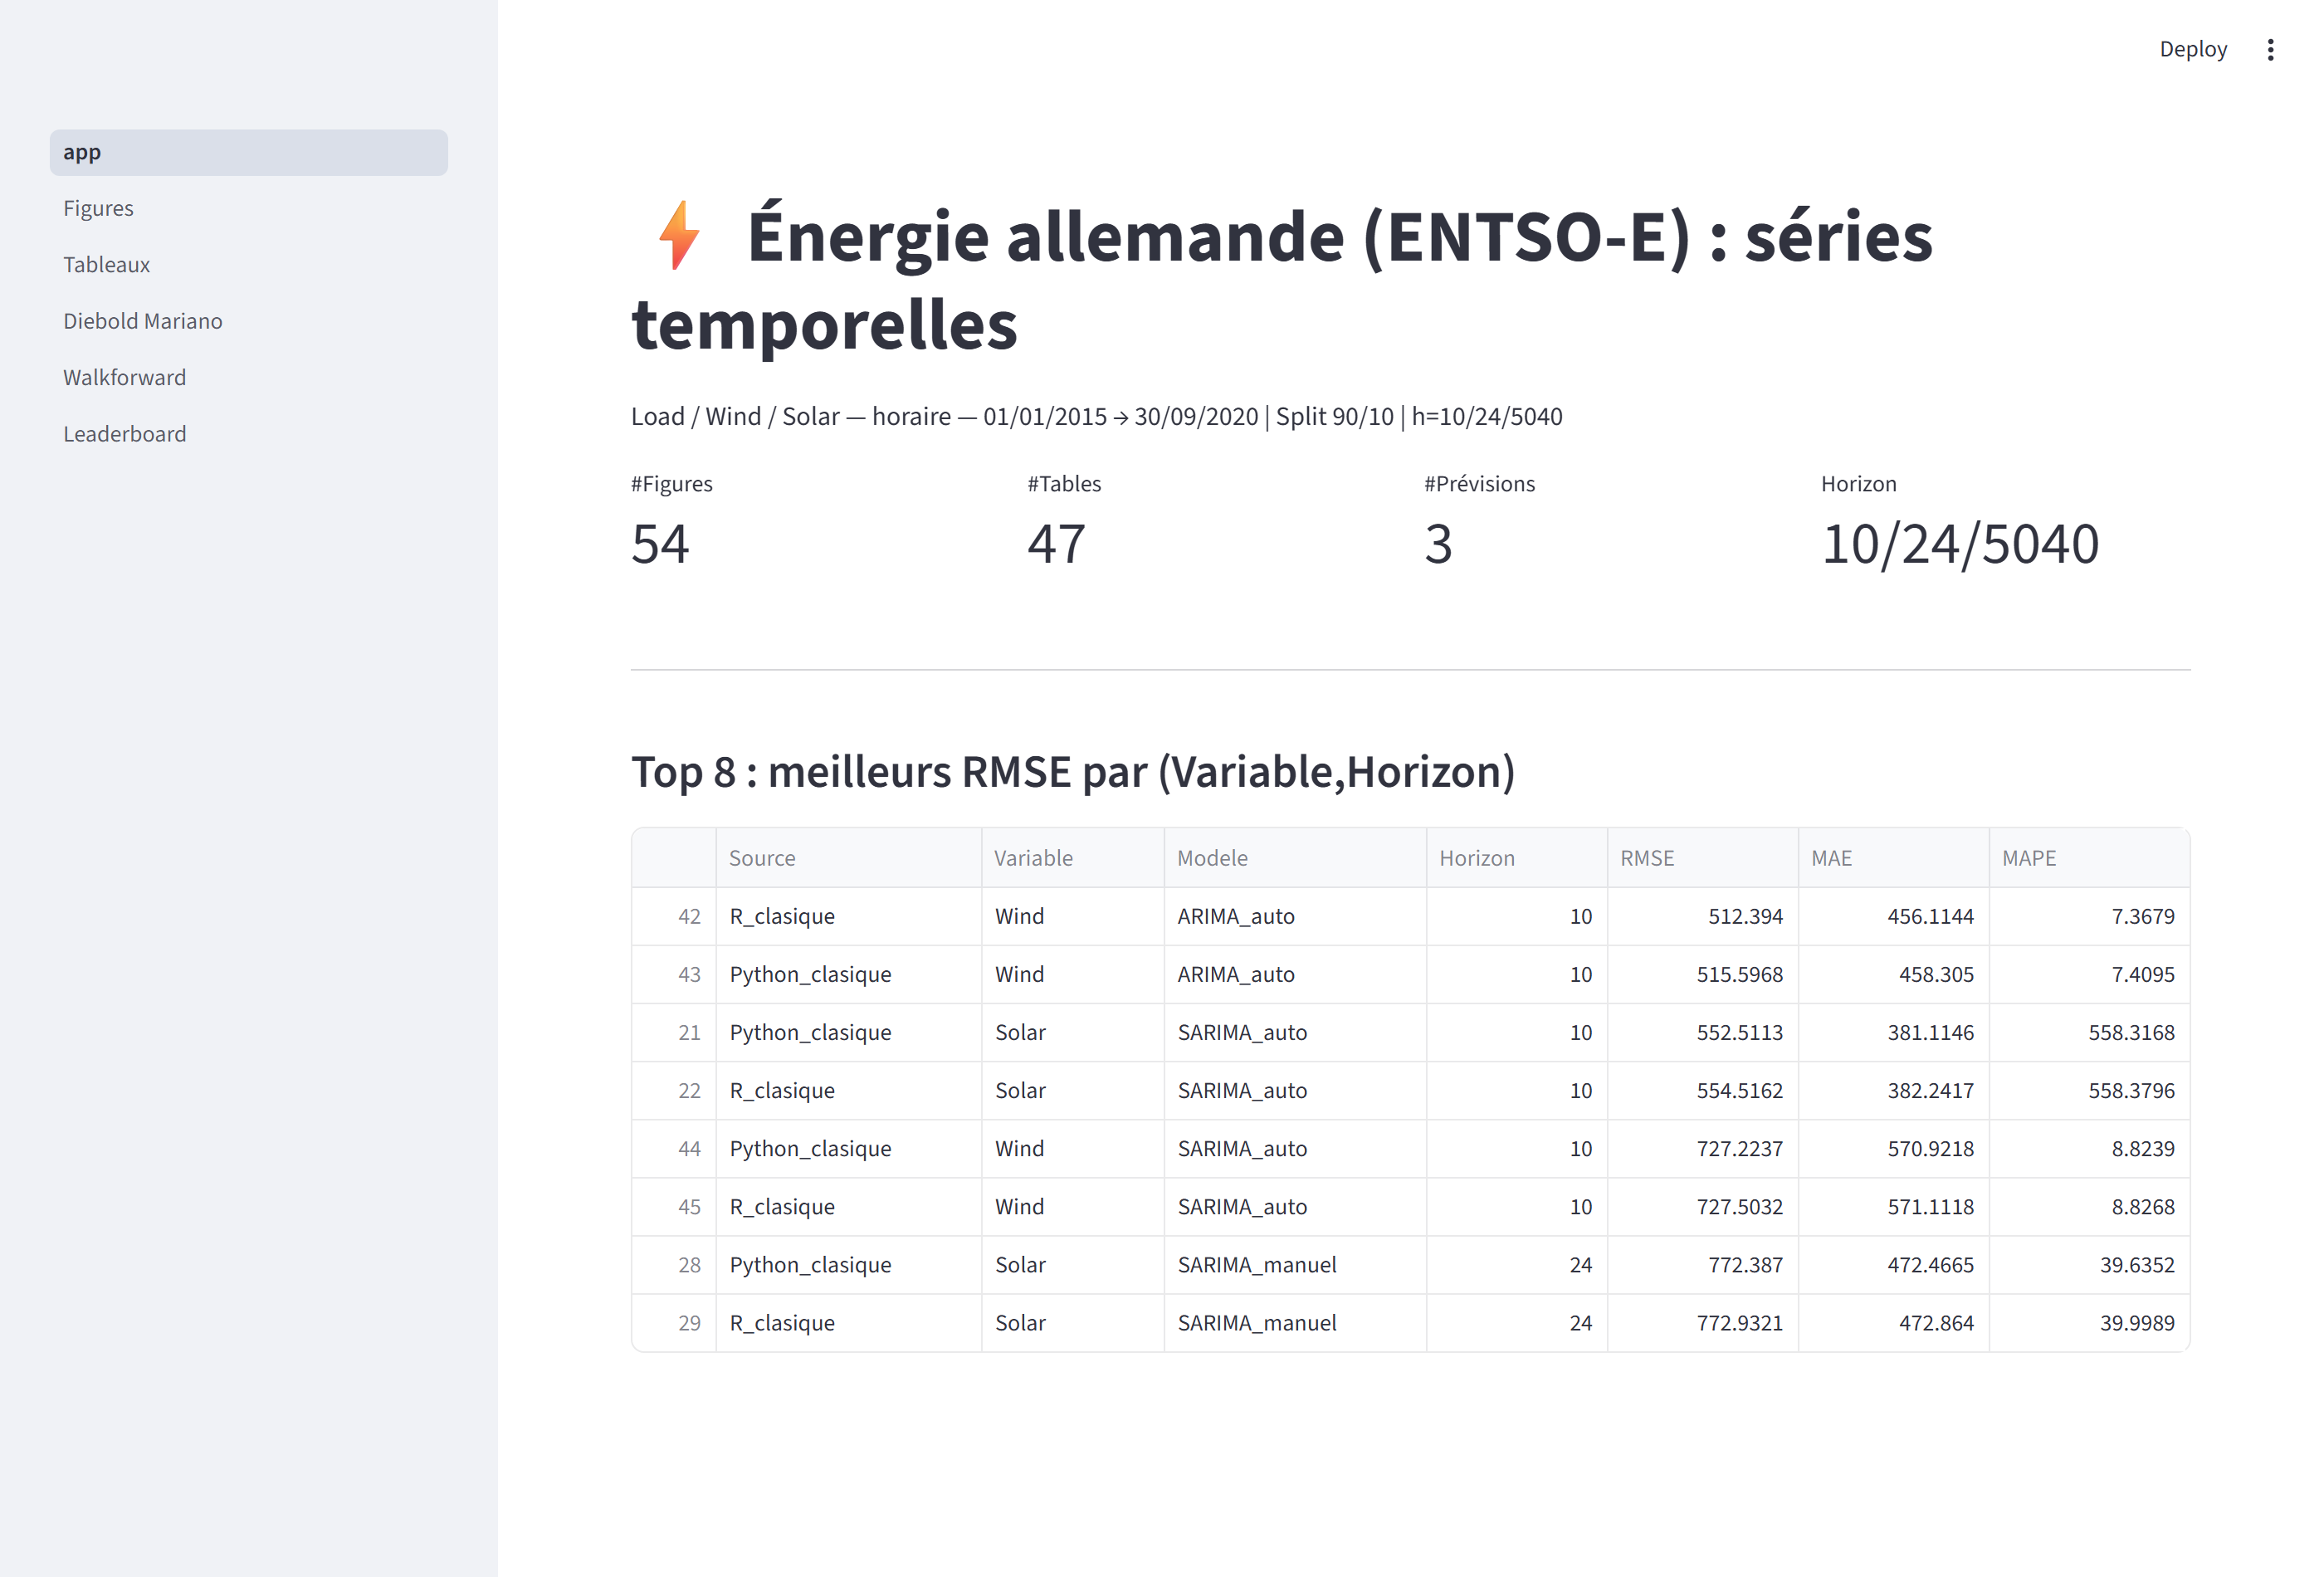
\includegraphics[width=0.9\textwidth]{dashboard_overview.png}
\caption{Interface Streamlit --- page « Vue d'ensemble ».}
\label{fig:dash_overview}
\end{figure}

\subsection{Page « Figures »}
Cette page constitue une galerie de l'ensemble des figures générées
(\(54\) fichiers \texttt{*.png}) avec leur légende.

\begin{figure}[H]
\centering
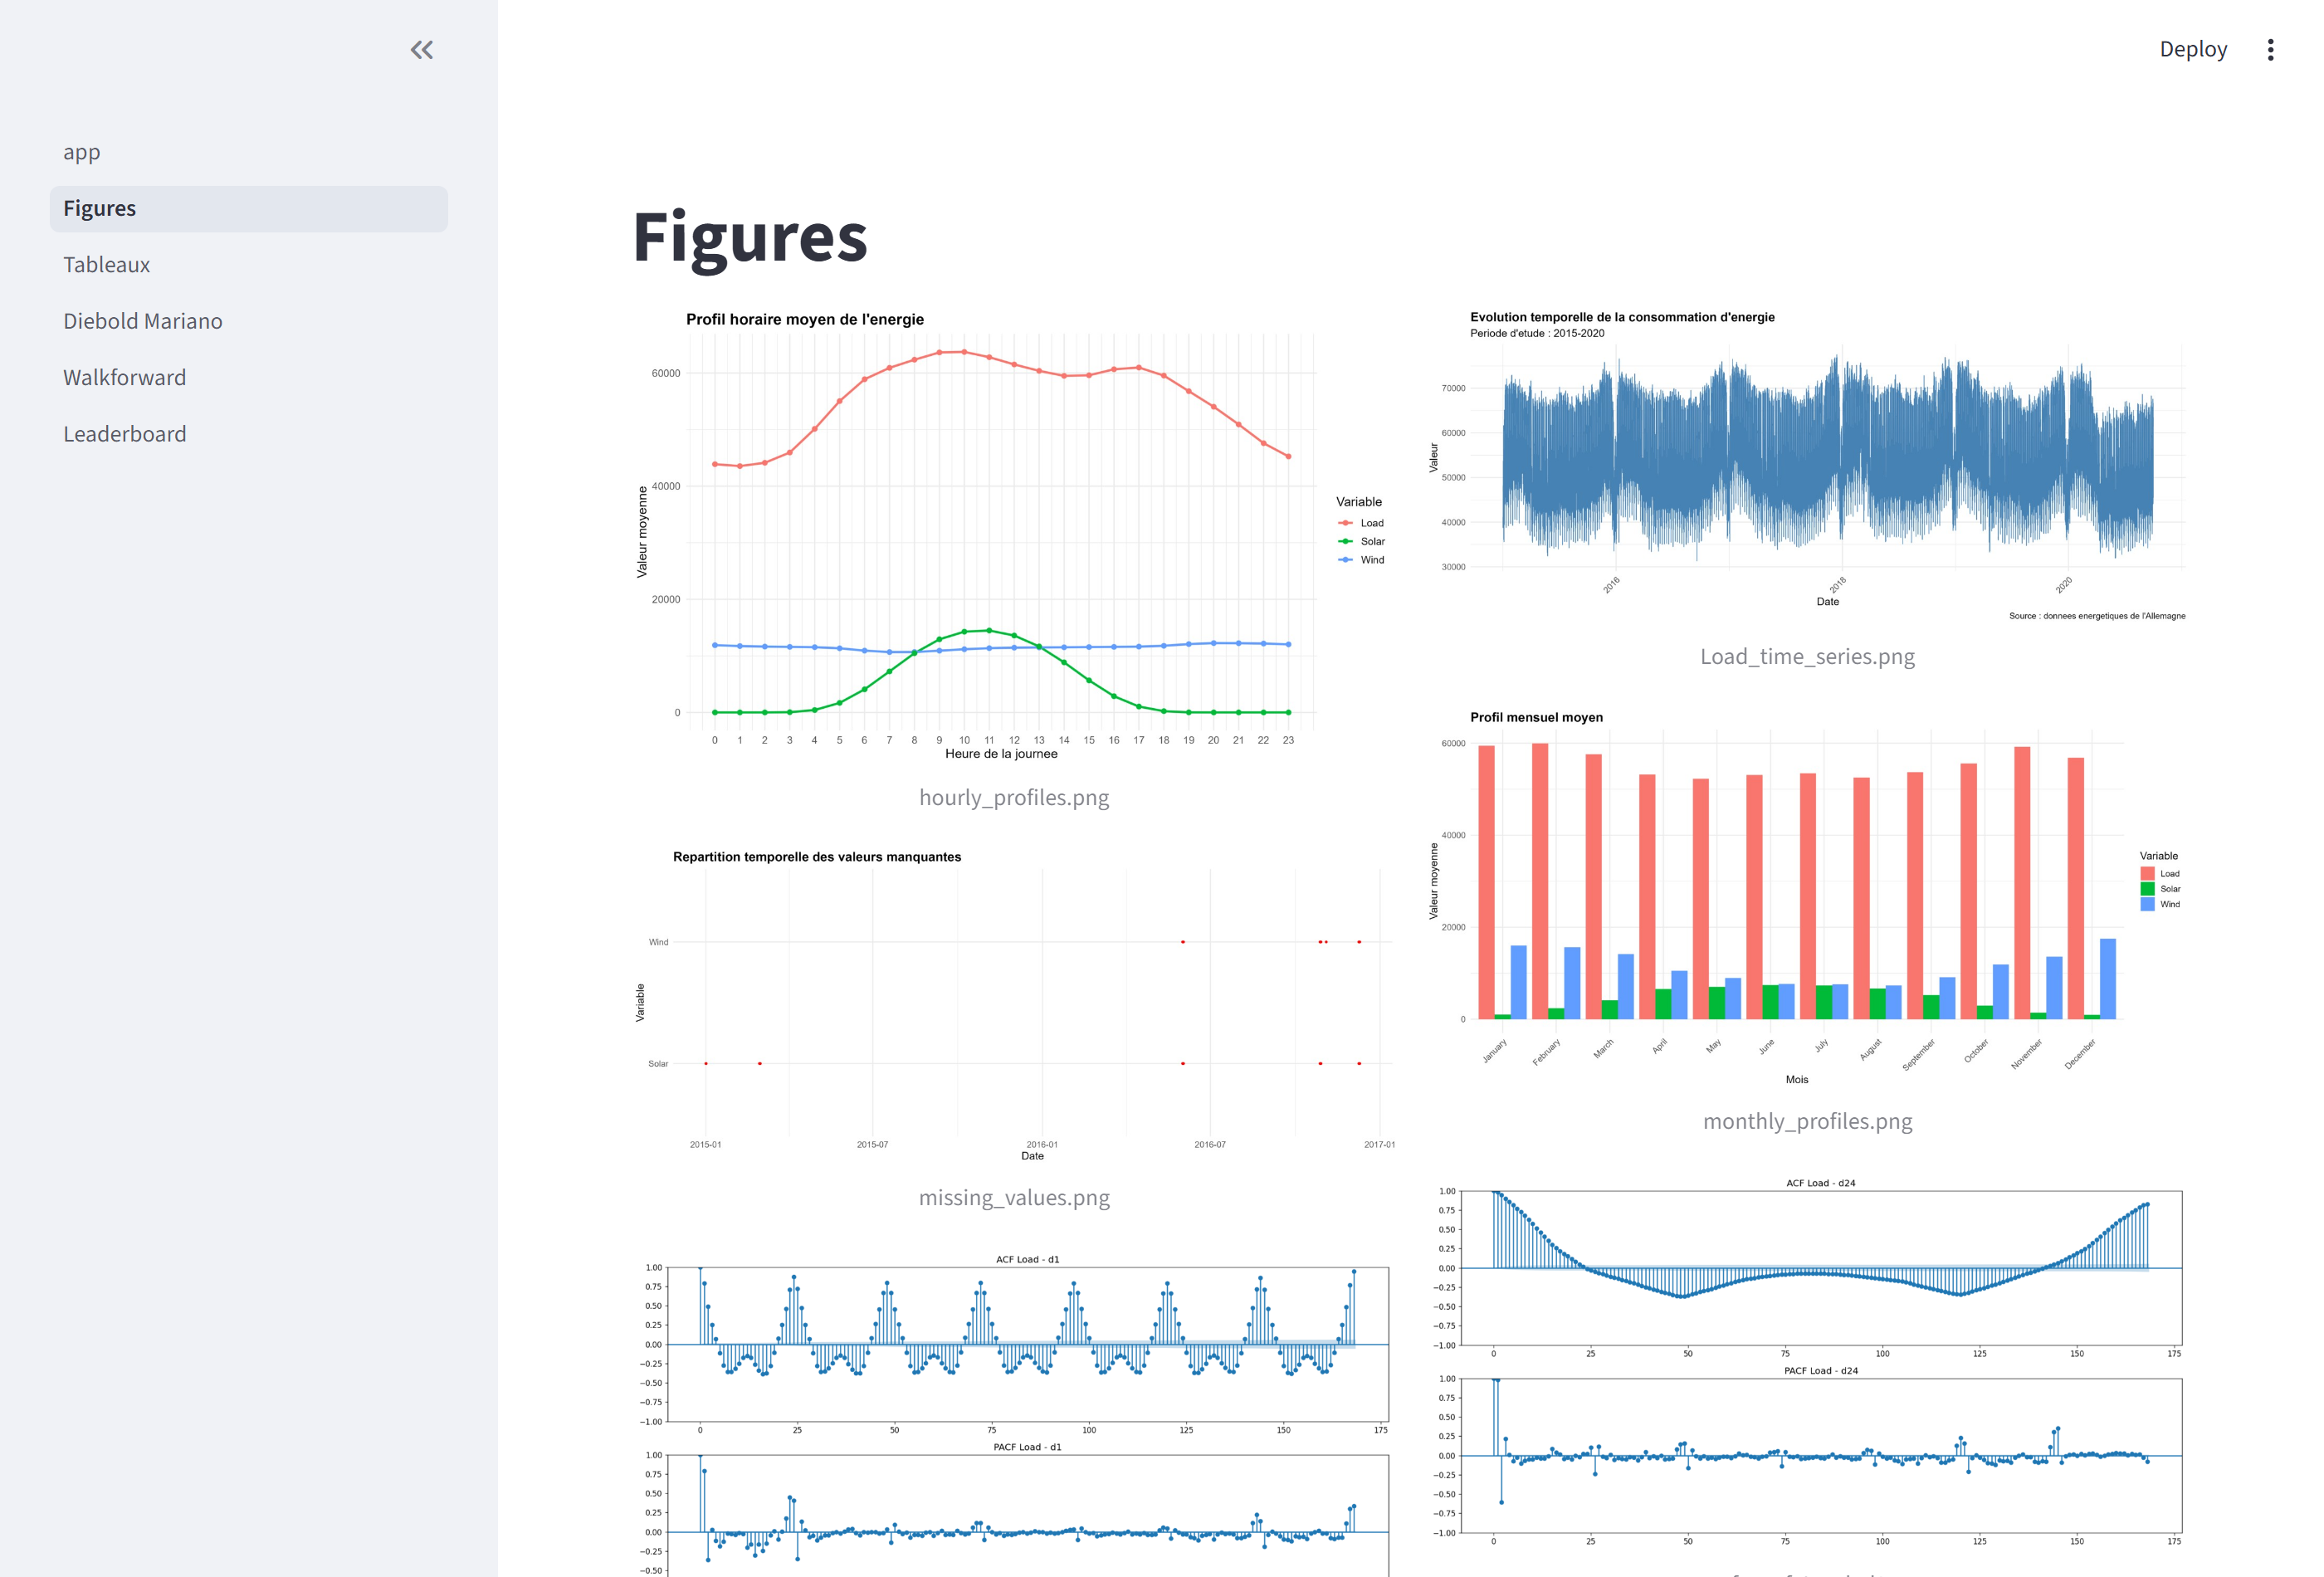
\includegraphics[width=0.9\textwidth]{dashboard_figures.png}
\caption{Interface Streamlit --- galerie « Figures ».}
\label{fig:dash_figures}
\end{figure}

\subsection{Page « Tableaux de résultats »}
Un sélecteur latéral permet de parcourir les \(47\) tables CSV produites, et
de visualiser n'importe quel tableau de résultats.

\begin{figure}[H]
\centering
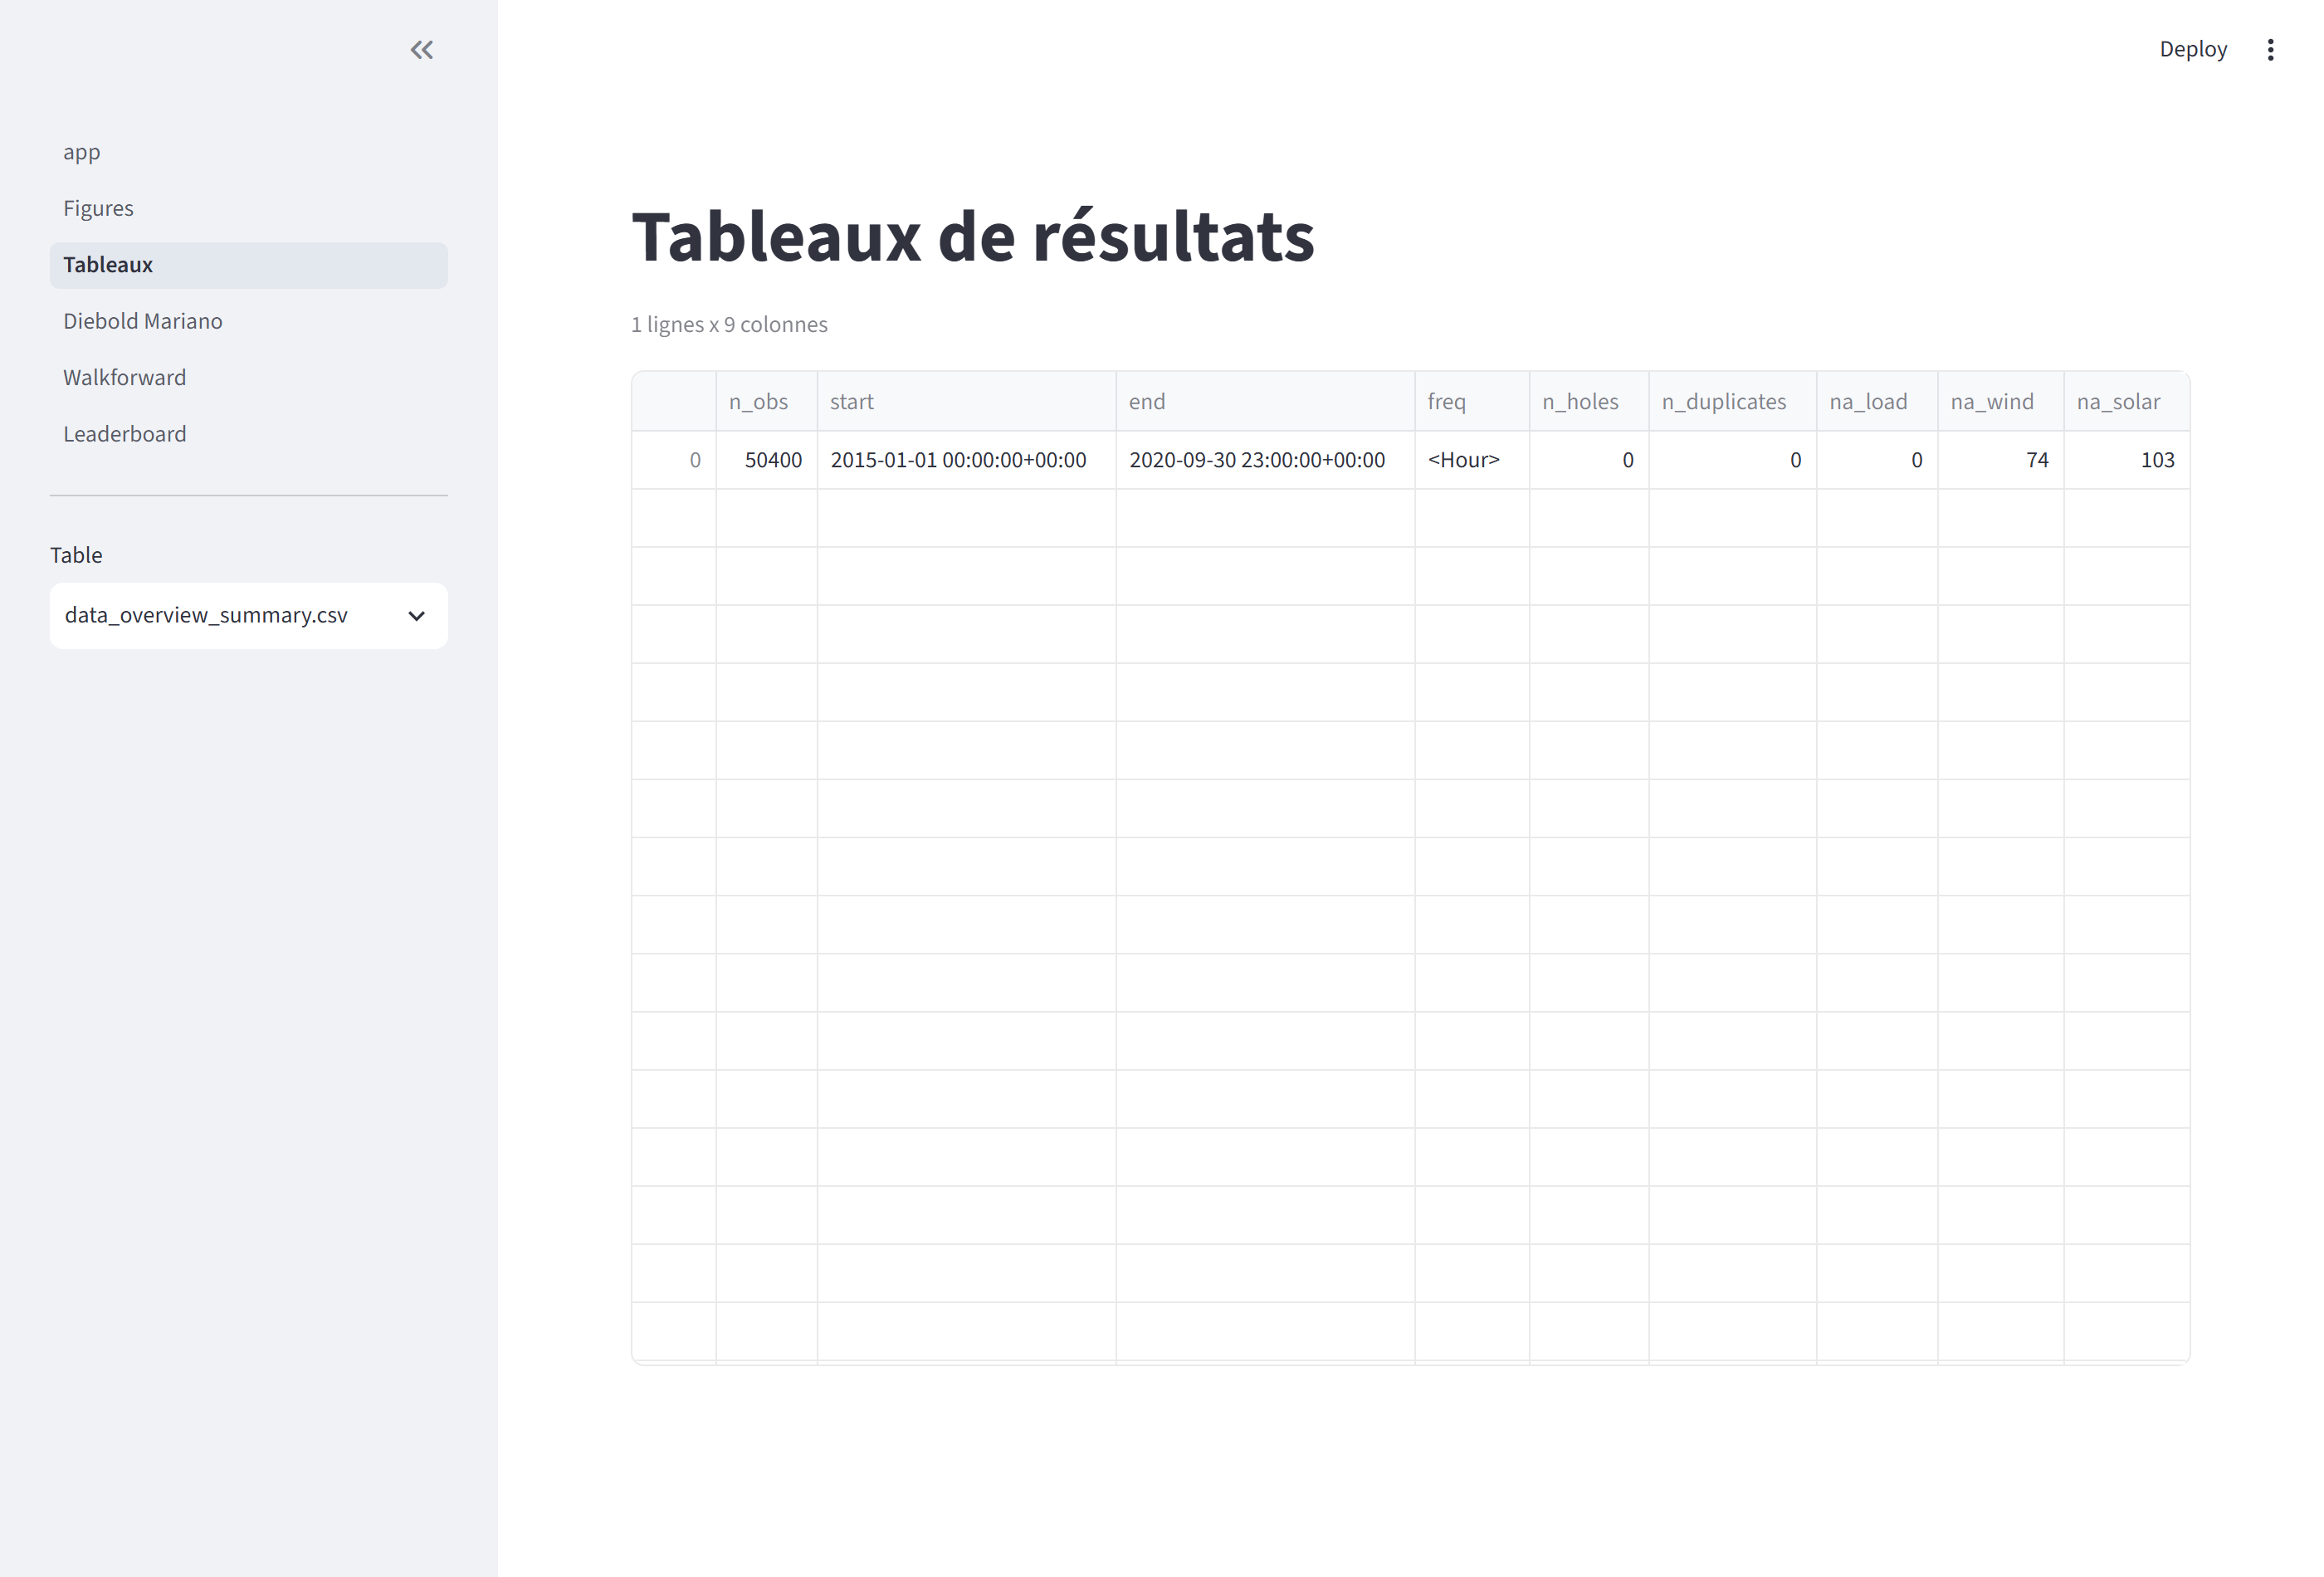
\includegraphics[width=0.9\textwidth]{dashboard_tableaux.png}
\caption{Interface Streamlit --- exploration des tableaux CSV.}
\label{fig:dash_tableaux}
\end{figure}

\subsection{Page « Diebold--Mariano »}
Cette page présente le tableau du test de Diebold--Mariano
(\texttt{py\_diebold\_mariano.csv}) comparant \textbf{toutes les paires} de
modèles du walk-forward (naïfs, SARIMA, LSTM, GRU).

\begin{figure}[H]
\centering
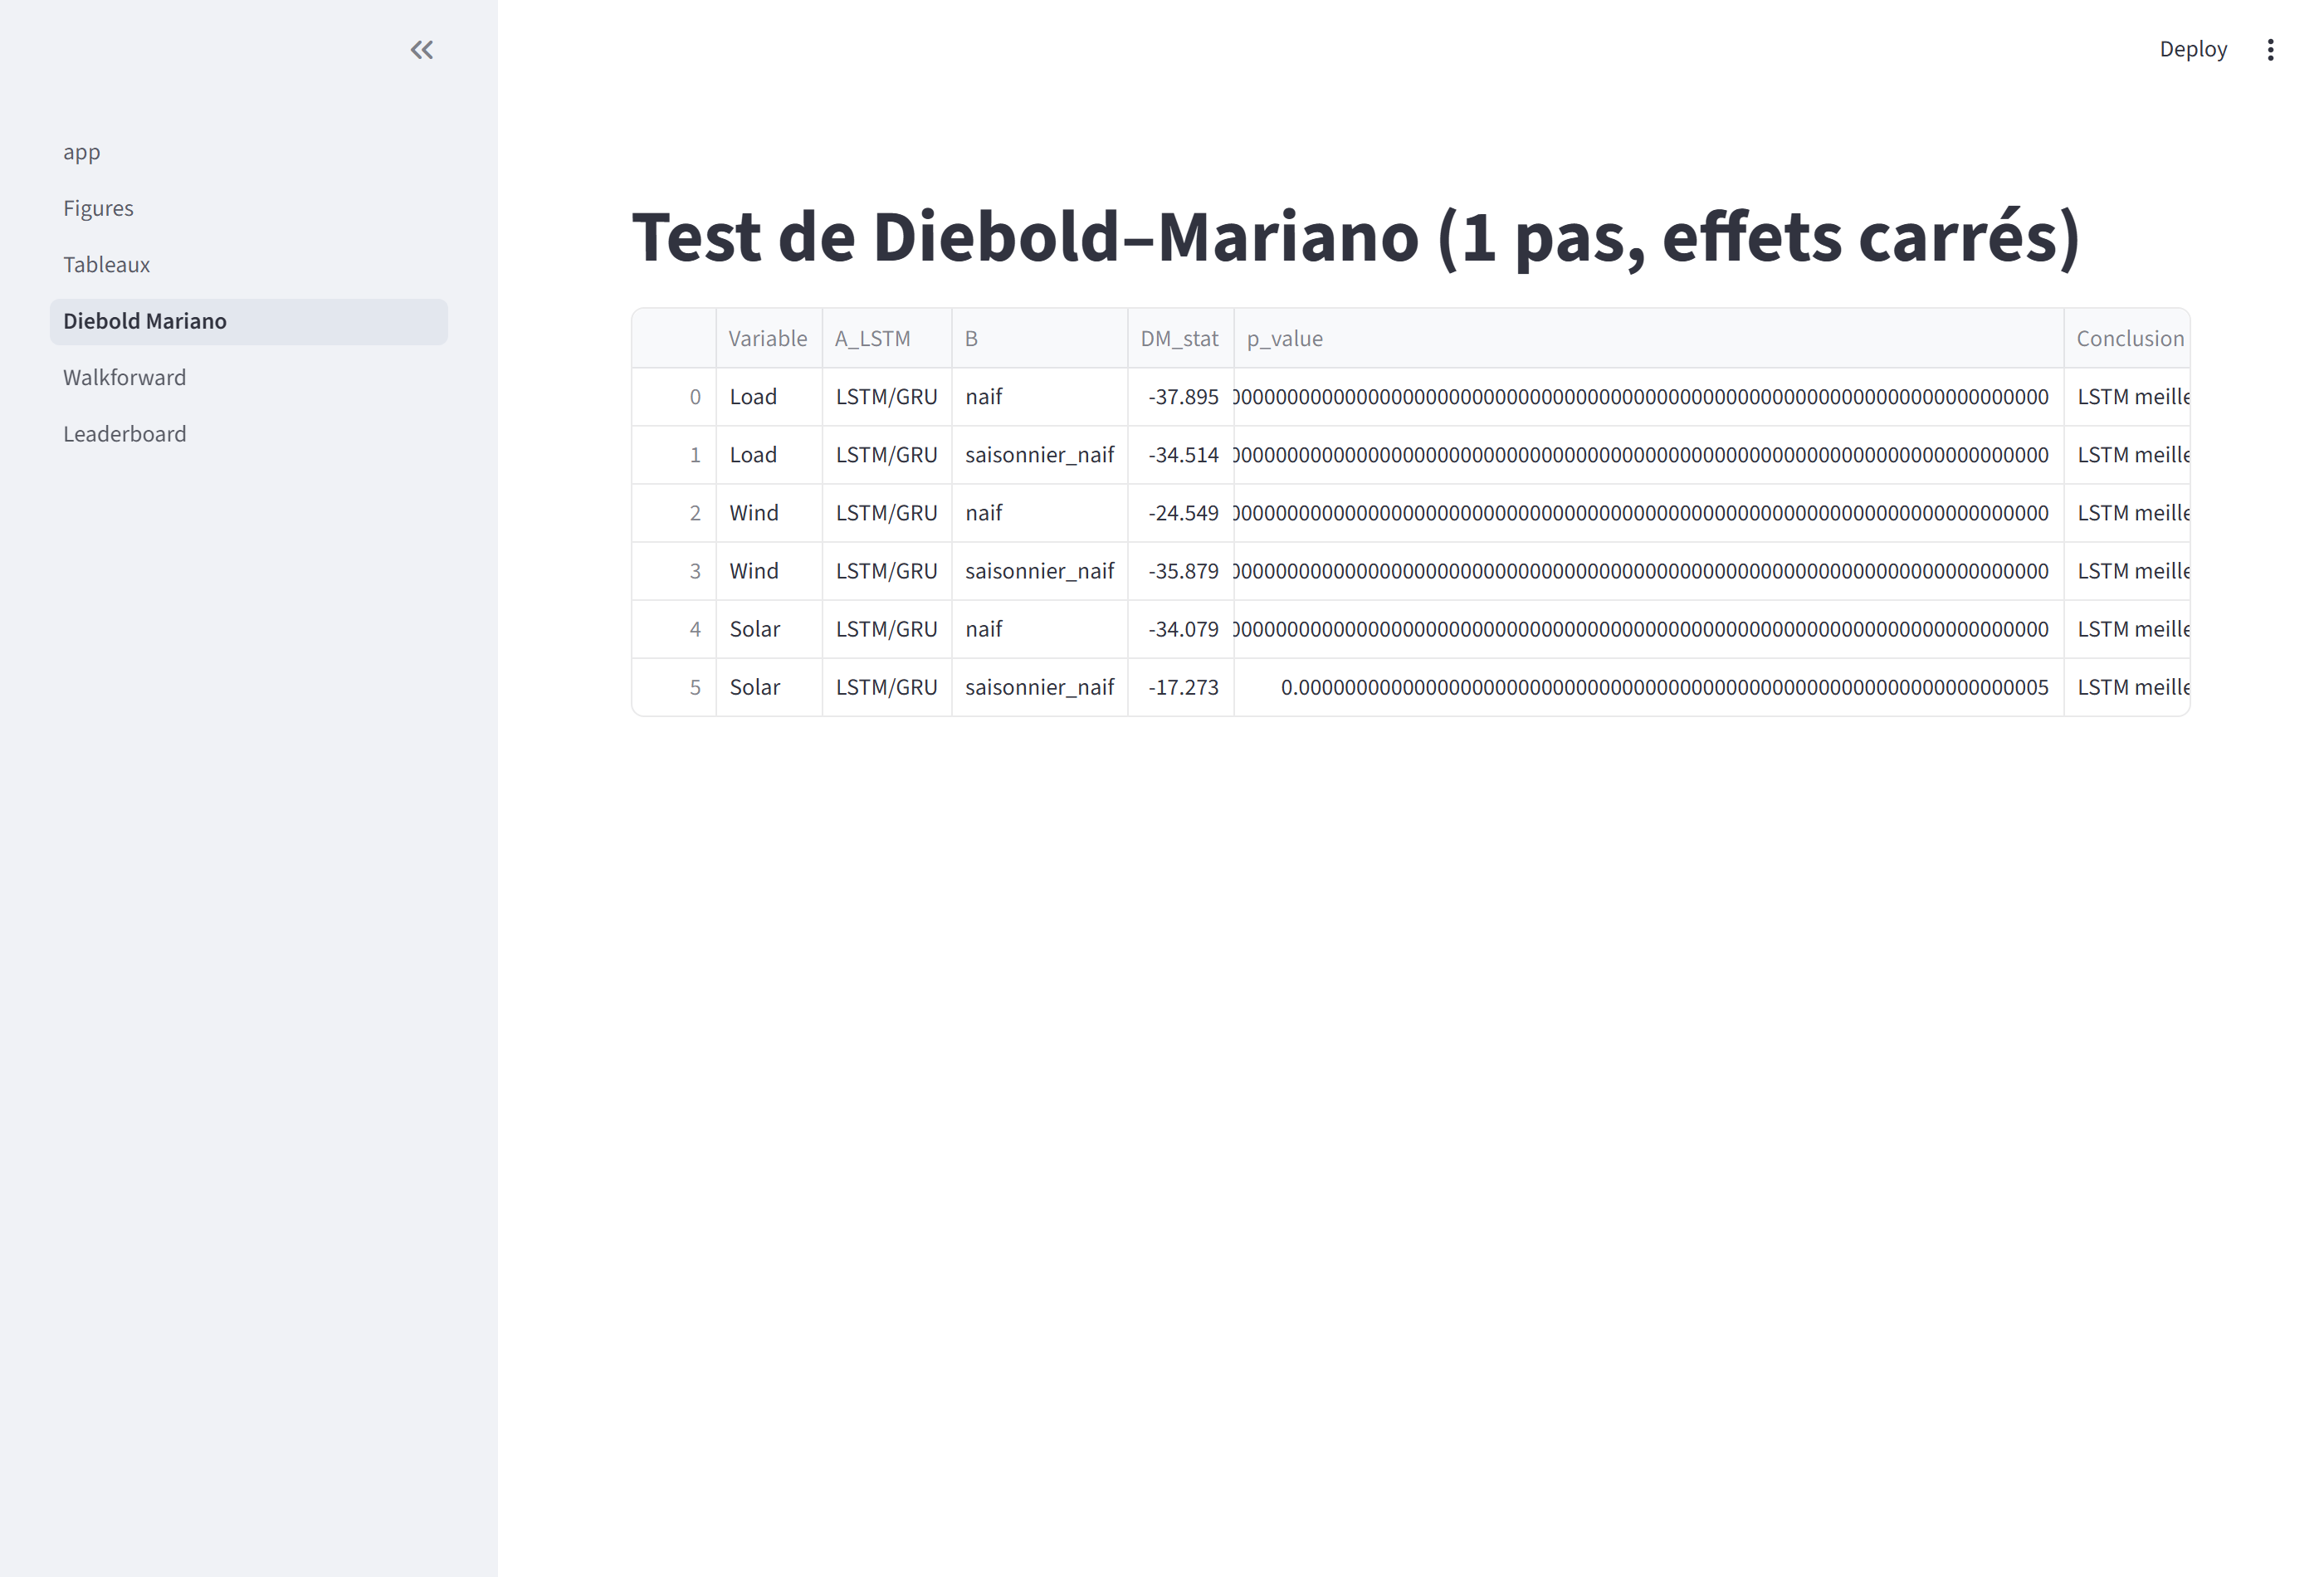
\includegraphics[width=0.9\textwidth]{dashboard_diebold_mariano.png}
\caption{Interface Streamlit --- test de Diebold--Mariano.}
\label{fig:dash_dm}
\end{figure}

\subsection{Page « Prévisions walk-forward »}
Un graphique interactif (Plotly) permet de sélectionner une variable et de
comparer la série observée aux prévisions à un pas (SARIMA, LSTM, GRU, naïf,
saisonnier naïf), avec une vue zoomée sur les 200 premiers points.

\begin{figure}[H]
\centering
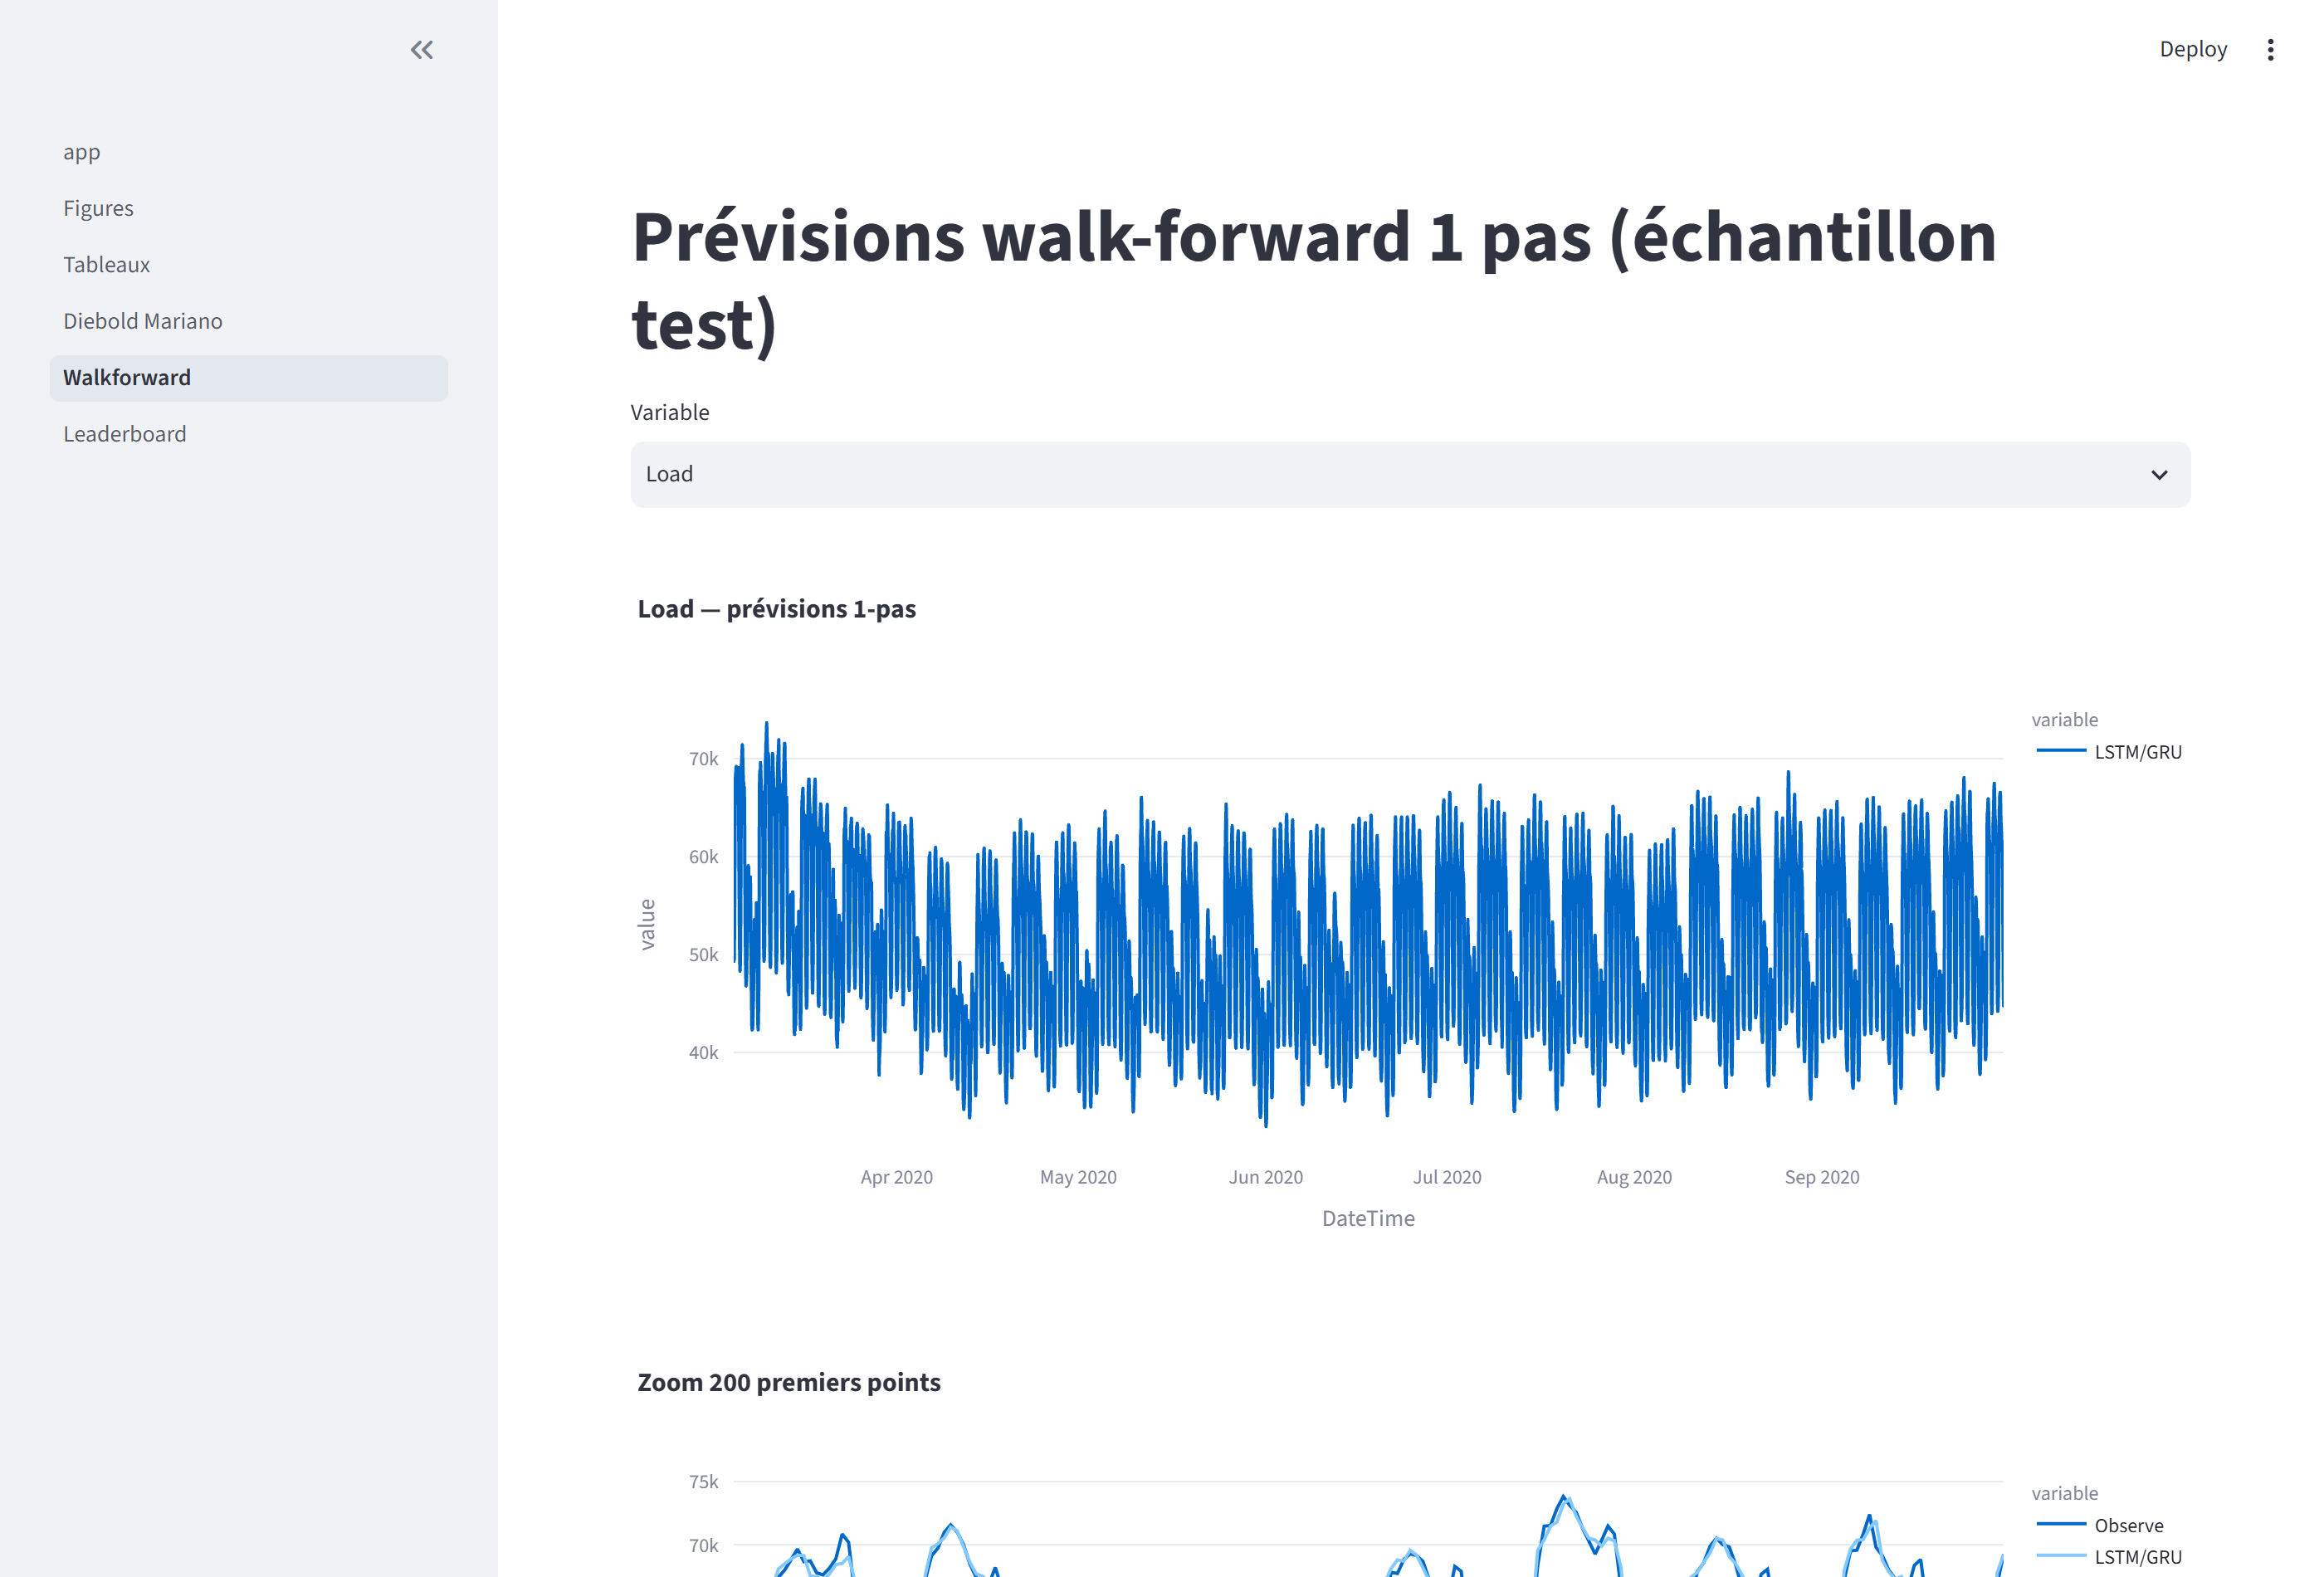
\includegraphics[width=0.9\textwidth]{dashboard_walkforward.png}
\caption{Interface Streamlit --- prévisions walk-forward.}
\label{fig:dash_wf}
\end{figure}

\subsection{Page « Leaderboard »}
Enfin, cette page classe par RMSE les modèles (R, Python classique, LSTM/GRU,
Prophet, hybride) pour une variable et un horizon choisis, sous forme de
tableau et de diagramme en barres interactif.

\begin{figure}[H]
\centering
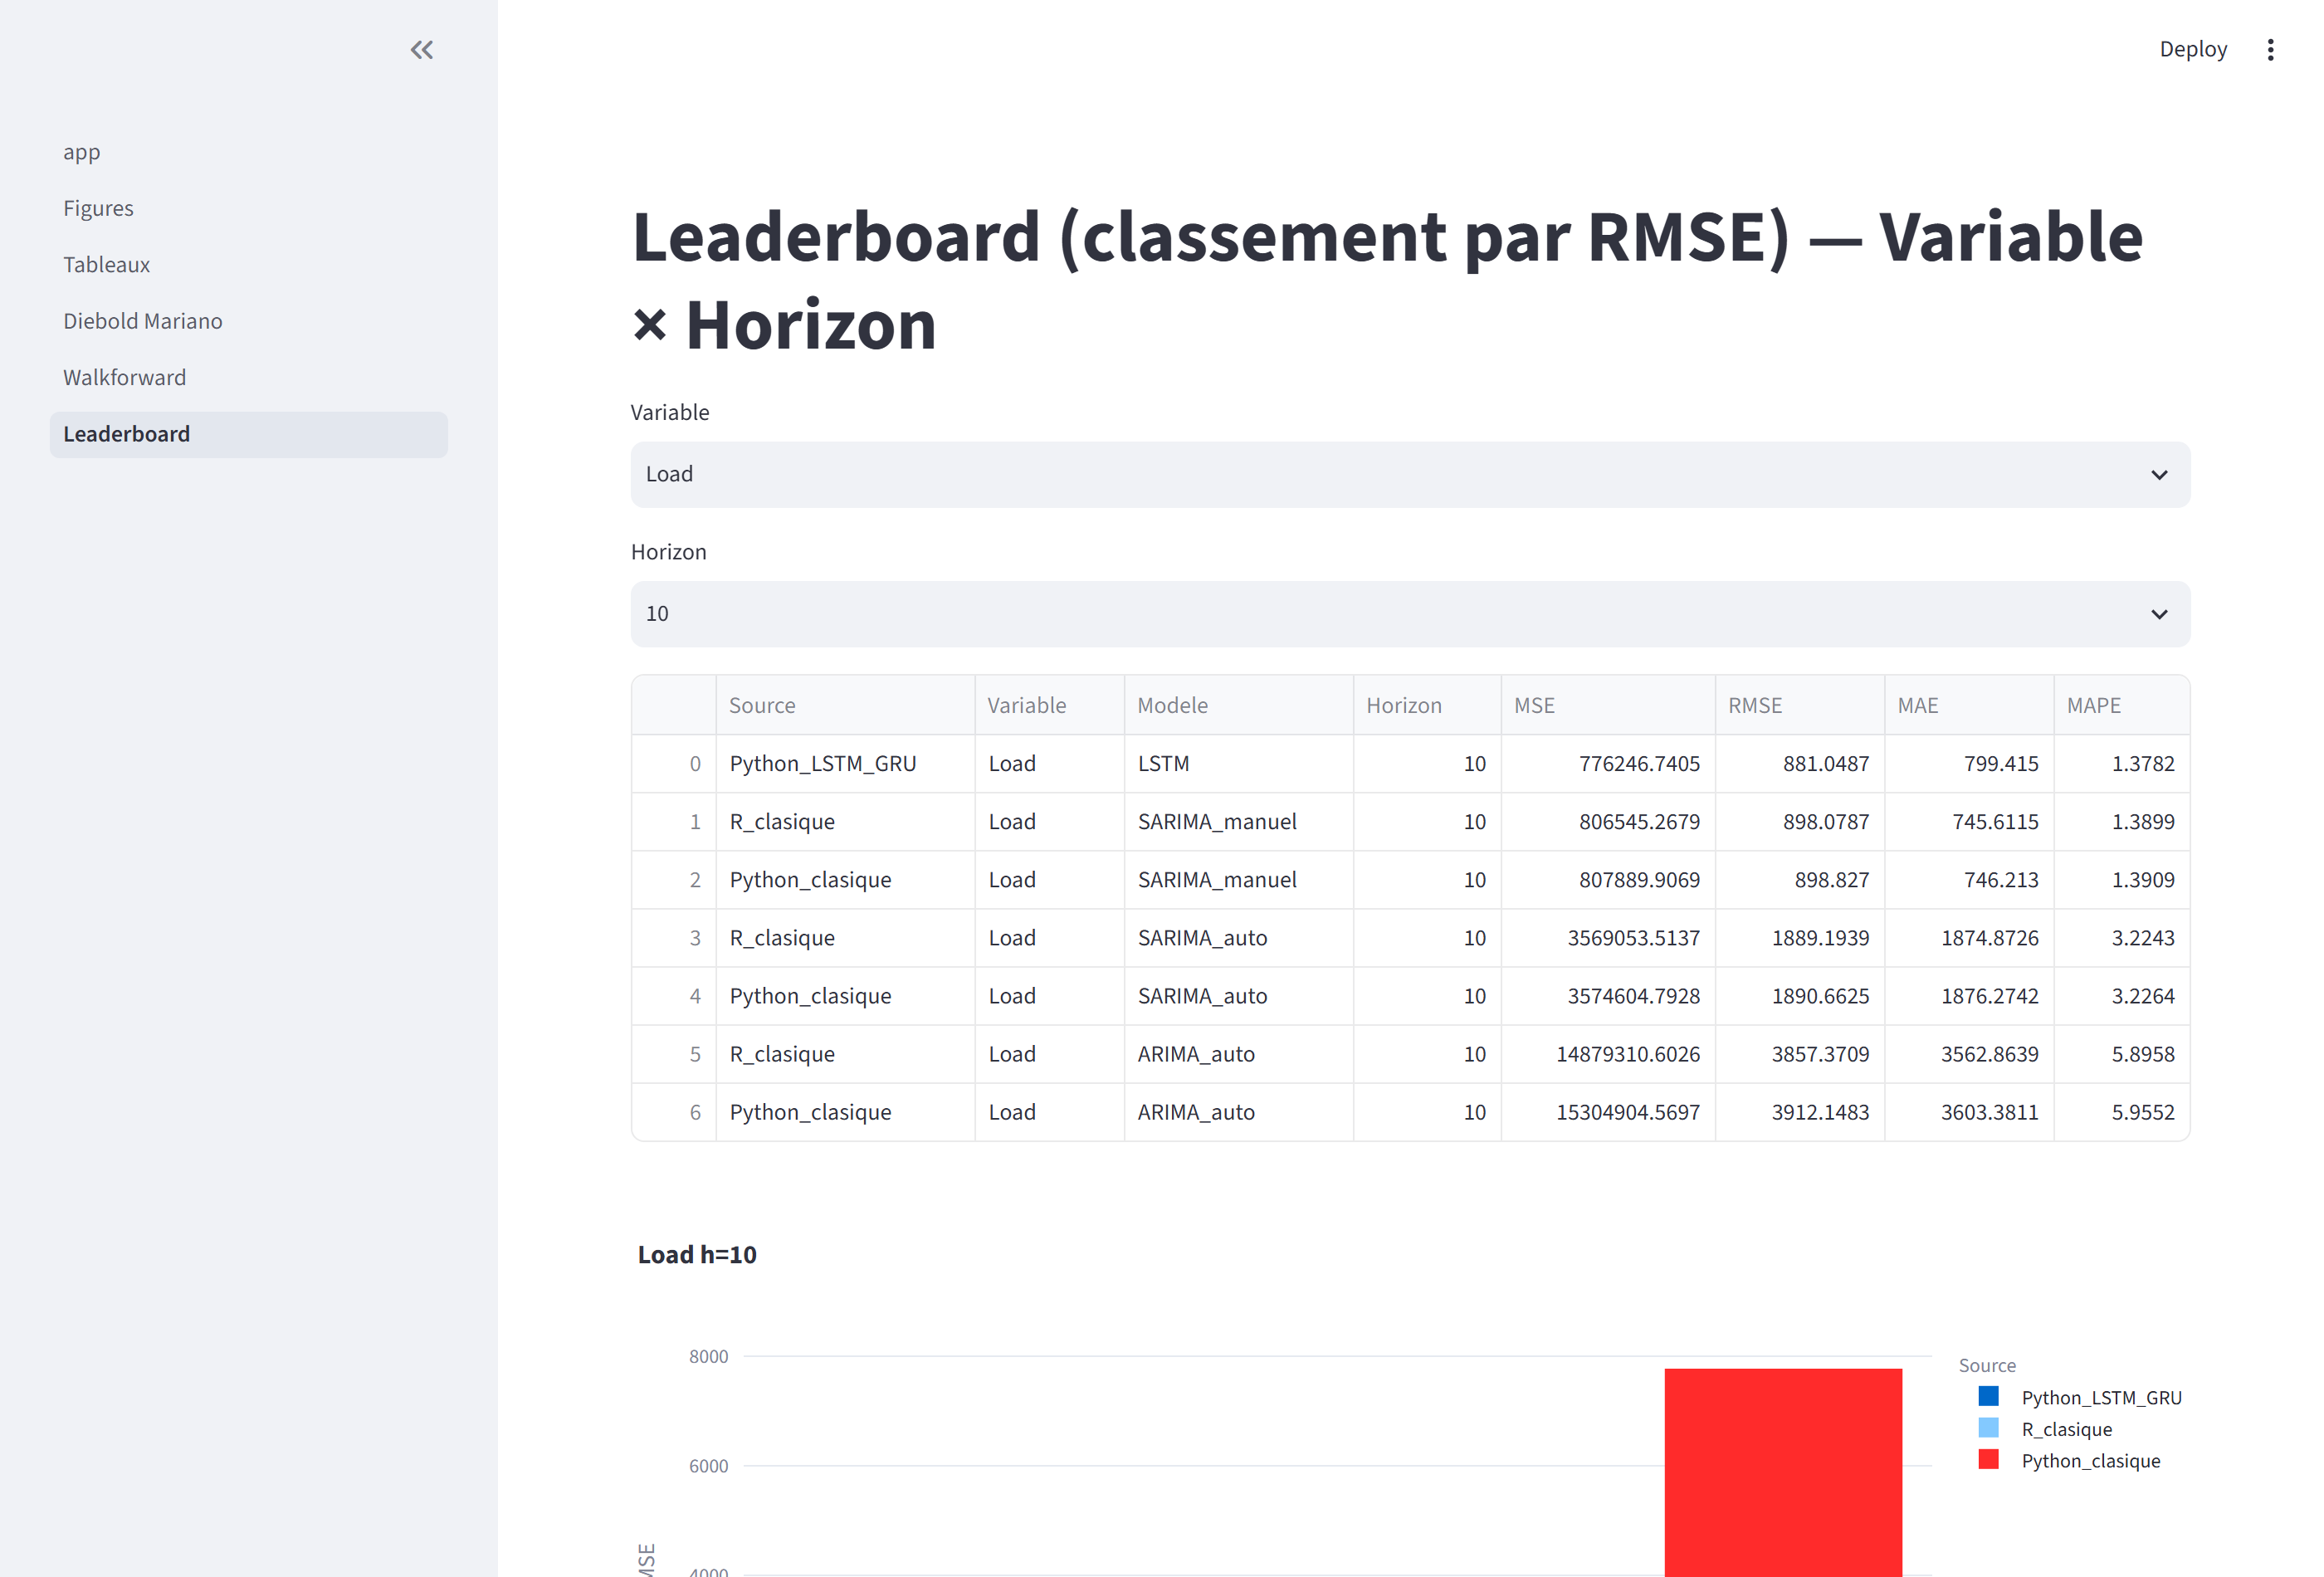
\includegraphics[width=0.9\textwidth]{dashboard_leaderboard.png}
\caption{Interface Streamlit --- leaderboard par variable et horizon.}
\label{fig:dash_leaderboard}
\end{figure}

\FloatBarrier

\section{Conclusion}
\label{sec:conclusion}

\subsection{Bilan des résultats}
Ce mini-projet a mis en \oe{}uvre, sur les trois séries énergétiques
allemandes (\texttt{Load}, \texttt{Wind}, \texttt{Solar}), une chaîne complète
d'analyse de séries temporelles, \textbf{duale R / Python}. Les principaux
résultats sont les suivants.

\begin{itemize}
  \item \textbf{Analyse exploratoire.} Les séries présentent une saisonnalité
        quotidienne (\(m=24\)) et hebdomadaire forte, une asymétrie marquée
        pour \texttt{Wind}/\texttt{Solar} et une saisonnalité annuelle
        opposée (éolien hivernal, solaire estival). Les séries brutes sont
        non stationnaires ; la différenciation \(d=1\) les rend stationnaires
        (ADF et KPSS concordants).

  \item \textbf{ARIMA/SARIMA.} Les ordres retenus par AICc sont
        \textbf{identiques} en R et en Python
        (\texttt{SARIMA\_manuel} pour \texttt{Load}/\texttt{Wind},
        \texttt{SARIMA\_auto} pour \texttt{Solar}). Les diagnostics rejettent
        l'absence d'autocorrélation, de non-normalité et d'effet ARCH, ce
        dernier point motivant le volet GARCH.

  \item \textbf{VAR / Granger / VECM.} L'ordre \(p=14\) est retenu par AIC.
        La causalité de Granger identifie une unique relation significative
        \textbf{\texttt{Wind} \(\to\) \texttt{Load}}. La cointégration de
        Johansen donne \(r=2\), et le VECM produit des vecteurs \(\beta\) et des
        vitesses \(\alpha\) \textbf{reproductibles} entre R et Python.

  \item \textbf{GARCH.} La volatilité des variations journalières est très
        persistante (\(\approx 0{,}99\) pour \texttt{Wind}) ; \texttt{Solar}
        est non covariation-stationnaire en GARCH(1,1)/GARCH(2,1), seul
        l'EGARCH(1,1) restant stable. Les innovations de Student capturent les
        queues épaisses.

  \item \textbf{LSTM/GRU.} Les réseaux récurrents apportent un gain mesurable
        à très long horizon (\(h=5\,040\) sur \texttt{Load} : RMSE \(7\,593\)
        contre \(65\,847\) pour le SARIMA) et surpassent nettement les naïfs
        en walk-forward un pas. À un pas, le \textbf{SARIMA} reste toutefois
        le meilleur modèle (test de Diebold--Mariano hautement significatif),
        ce qui conforte l'intérêt des approches hybrides.

  \item \textbf{Reproductibilité.} Les deux implémentations (R et Python)
        produisent des métriques quasi identiques (écarts \(<0{,}5\,\%\)),
        validant la démarche de double codage.
\end{itemize}

\subsection{Limites}
\begin{enumerate}
  \item \textbf{Horizon long.} À \(h=5\,040\), les prévisions récursives des
        modèles classiques divergent ; seule la comparaison
        inter-modèles reste informative.
  \item \textbf{MAPE et \texttt{Solar}.} La proximité de zéro (nuit) rend le
        MAPE ininterprétable ; il doit être systématiquement complété par
        RMSE/MAE.
  \item \textbf{Saisonnalité tronquée.} Seul \(m=24\) est modélisé
        explicitement ; la saisonnalité hebdomadaire (\(m=168\)) et annuelle
        ne sont pas prises en compte par les modèles ARIMA/SARIMA, ce qui
        limite la qualité à moyen terme.
  \item \textbf{Ordre VAR élevé.} \(p=14\) sur \(\approx 1\,890\) jours
        d'apprentissage peut conduire à un sur-ajustement ; les critères
        HQ/SC suggèrent un ordre plus faible.
  \item \textbf{Période de test COVID.} Le test débute le \(5\) mars 2020,
        à l'entrée de la crise sanitaire : la rupture de régime affecte
        nécessairement les performances.
  \item \textbf{Monovariable pour le LSTM.} Les réseaux sont entraînés série
        par série, sans exploiter l'information croisée (Wind/Solar/Load),
        pourtant mise en évidence par le VECM.
\end{enumerate}

\subsection{Perspectives}
\begin{enumerate}
  \item Intégrer des \textbf{régresseurs de Fourier} (saisonnalités 24/168)
        ou un SARIMA à \(m=168\) sur fenêtres plus courtes.
  \item Passer à des LSTM/GRU \textbf{multivariés} (entrées conjointes des
        trois séries) et ajouter des variables exogènes (température, vent,
        irradiance).
  \item Conduire le test de \textbf{Diebold--Mariano entre SARIMA et LSTM}
        sur les trajectoires \(h>1\), et non seulement en un pas.
  \item Étudier des modèles de volatilité multivariés (DCC-GARCH) pour la
        dépendance conditionnelle entre séries.
  \item Produire des \textbf{intervalles de prévision} calibrés (prévision
        probabiliste) plutôt que des points.
  \item Déployer l'ensemble dans un \emph{dashboard} interactif
        (Streamlit, déjà présent dans \texttt{dashboard/}) pour la
        vulgarisation.
\end{enumerate}

En définitive, le socle classique (ARIMA, VAR/VECM, GARCH) et son extension
profonde (LSTM/GRU) ont été implémentés de façon cohérente et reproductible,
et comparés rigoureusement. Les résultats confirment l'intérêt des approches
hybrides : modèles classiques pour les horizons courts et interprétables,
modèles profonds pour les horizons longs, l'ensemble devant être complété par
une modélisation explicite des saisonnalités et des relations multivariées.

\section{Annexes}

\subsection{Structure du projet et reproductibilité}
L'ensemble du travail est contenu dans le dépôt
\texttt{TimeSeries\_Project} :
\begin{itemize}
  \item \texttt{R/} : six scripts séquentiels ---
        \texttt{01\_data\_preparation.R}, \texttt{02\_EDA.R},
        \texttt{03\_diagnostics.R}, \texttt{04\_ARIMA\_SARIMA.R},
        \texttt{05\_VAR\_VECM.R}, \texttt{06\_GARCH.R} ;
  \item \texttt{Python/} : transposition
        (\texttt{arima\_var.py}, \texttt{arima\_intervals.py},
        \texttt{garch.py}, \texttt{lstm\_gru.py},
        \texttt{prophet\_model.py}, \texttt{hybrid\_arima\_lstm.py},
        \texttt{evaluation.py}) ;
  \item \texttt{data/processed/} : données préparées ;
  \item \texttt{results/tables/}, \texttt{results/figures/},
        \texttt{results/forecasts/}, \texttt{results/models/} : sorties
        (préfixes \texttt{R\_} et \texttt{py\_}) ;
  \item \texttt{rapport/} : le présent rapport \LaTeX{} ;
  \item \texttt{dashboard/} : prototype Streamlit ;
  \item \texttt{notebooks/} : \texttt{analyse\_complete.Rmd} et
        \texttt{analyse\_complete.ipynb} (EDA) ;
  \item \texttt{notebooks/analyse\_complete\_full.ipynb} : notebook
        \textbf{bout-en-bout} couvrant les dix étapes du pipeline (données,
        EDA, stationnarité, ARIMA/SARIMA, GARCH, VAR/VECM, LSTM/GRU, Prophet
        et hybride, évaluation, volet IA).
\end{itemize}
Toutes les métriques et figures du rapport sont régénérables en exécutant les
scripts dans l'ordre (voir le \texttt{README.md} de la racine).

\subsection{Tableaux de synthèse complémentaires}

\begin{table}[H]
\centering
\caption{Statistiques descriptives (version R).
Source : \texttt{descriptive\_statistics.csv}.}
\label{tab:desc_r}
\small
\begin{tabular}{lrrrrrr}
\toprule
Variable & $n$ & NA & Moyenne & Médiane & Min & Max \\
\midrule
\texttt{Load}  & 50\,400 & 0 & 55\,492{,}5 & 55\,092 & 31\,307 & 77\,549 \\
\texttt{Wind}  & 50\,326 & 74 & 11\,552{,}2 & 9\,015 & 135 & 46\,064 \\
\texttt{Solar} & 50\,297 & 103 & 4\,566{,}0 & 173 & 0 & 32\,947 \\
\bottomrule
\end{tabular}
\end{table}

{\small
\begin{longtable}{lrrr}
\caption{Profil horaire moyen (MW). Source : \texttt{hourly\_summary.csv}.}
\label{tab:hourly}\\
\toprule
Heure & \texttt{Load} & \texttt{Wind} & \texttt{Solar} \\
\midrule
\endfirsthead
\toprule
Heure & \texttt{Load} & \texttt{Wind} & \texttt{Solar} \\
\midrule
\endhead
\bottomrule
\endlastfoot
0 & 43\,882 & 11\,884 & 0{,}01 \\
1 & 43\,553 & 11\,737 & 0{,}01 \\
2 & 44\,134 & 11\,640 & 0{,}31 \\
3 & 45\,950 & 11\,589 & 41{,}67 \\
4 & 50\,132 & 11\,537 & 426{,}92 \\
5 & 55\,042 & 11\,337 & 1\,688{,}08 \\
6 & 58\,898 & 10\,927 & 4\,081{,}74 \\
7 & 60\,921 & 10\,670 & 7\,253{,}83 \\
8 & 62\,353 & 10\,676 & 10\,471{,}87 \\
9 & 63\,641 & 10\,914 & 12\,925{,}39 \\
10 & 63\,734 & 11\,171 & 14\,278{,}53 \\
11 & 62\,801 & 11\,359 & 14\,482{,}78 \\
12 & 61\,518 & 11\,451 & 13\,595{,}15 \\
13 & 60\,384 & 11\,494 & 11\,661{,}40 \\
14 & 59\,499 & 11\,515 & 8\,850{,}42 \\
15 & 59\,599 & 11\,556 & 5\,666{,}05 \\
16 & 60\,663 & 11\,588 & 2\,868{,}91 \\
17 & 60\,975 & 11\,635 & 1\,039{,}00 \\
18 & 59\,545 & 11\,783 & 226{,}68 \\
19 & 56\,794 & 12\,080 & 12{,}27 \\
20 & 54\,040 & 12\,258 & 0{,}87 \\
21 & 50\,916 & 12\,240 & 0{,}86 \\
22 & 47\,596 & 12\,178 & 0{,}01 \\
23 & 45\,251 & 12\,037 & 0{,}01 \\
\end{longtable}
}

\begin{table}[H]
\centering
\caption{Profil hebdomadaire moyen (MW). Source : \texttt{weekly\_summary.csv}.}
\label{tab:weekly}
\small
\resizebox{\textwidth}{!}{%
\begin{tabular}{lrrr}
\toprule
Jour & \texttt{Load} & \texttt{Wind} & \texttt{Solar} \\
\midrule
Lundi     & 57\,523 & 11\,492 & 4\,557 \\
Mardi     & 59\,241 & 11\,737 & 4\,513 \\
Mercredi  & 59\,455 & 11\,672 & 4\,665 \\
Jeudi     & 58\,964 & 11\,337 & 4\,575 \\
Vendredi  & 57\,742 & 10\,957 & 4\,561 \\
Samedi    & 49\,619 & 11\,777 & 4\,517 \\
Dimanche  & 45\,902 & 11\,892 & 4\,575 \\
\bottomrule
\end{tabular}}
\end{table}

\begin{table}[H]
\centering
\caption{Profil mensuel moyen (MW). Source : \texttt{monthly\_summary.csv}.}
\label{tab:monthly}
\small
\resizebox{\textwidth}{!}{%
\begin{tabular}{lrrr}
\toprule
Mois & \texttt{Load} & \texttt{Wind} & \texttt{Solar} \\
\midrule
Janvier   & 59\,446 & 16\,029 & 1\,029 \\
Février   & 59\,975 & 15\,656 & 2\,397 \\
Mars      & 57\,606 & 14\,185 & 4\,114 \\
Avril     & 53\,209 & 10\,571 & 6\,552 \\
Mai       & 52\,285 & 8\,964 & 7\,039 \\
Juin      & 53\,111 & 7\,704 & 7\,461 \\
Juillet   & 53\,453 & 7\,608 & 7\,378 \\
Août      & 52\,566 & 7\,340 & 6\,683 \\
Septembre & 53\,705 & 9\,134 & 5\,270 \\
Octobre   & 55\,621 & 11\,911 & 2\,947 \\
Novembre  & 59\,232 & 13\,593 & 1\,446 \\
Décembre  & 56\,849 & 17\,515 & 967 \\
\bottomrule
\end{tabular}}
\end{table}

\begin{table}[H]
\centering
\caption{Évolution annuelle moyenne (MW). Source : \texttt{yearly\_summary.csv}.}
\label{tab:yearly}
\small
\begin{tabular}{lrrr}
\toprule
Année & \texttt{Load} & \texttt{Wind} & \texttt{Solar} \\
\midrule
2015 & 54\,737 & 8\,810 & 3\,986 \\
2016 & 55\,441 & 8\,718 & 3\,946 \\
2017 & 56\,178 & 11\,720 & 4\,096 \\
2018 & 56\,952 & 12\,393 & 4\,707 \\
2019 & 55\,990 & 14\,133 & 4\,785 \\
2020 & 53\,048 & 14\,178 & 6\,304 \\
\bottomrule
\end{tabular}
\end{table}

{\small
\begin{longtable}{lllrrrr}
\caption{Métriques ARIMA/SARIMA (Python) --- confirmation des valeurs R.
Source : \texttt{py\_arima\_metrics.csv}.}
\label{tab:arima_metrics_py}\\
\toprule
Variable & Modèle & $h$ & MSE & RMSE & MAE & MAPE (\%) \\
\midrule
\endfirsthead
\toprule
Variable & Modèle & $h$ & MSE & RMSE & MAE & MAPE (\%) \\
\midrule
\endhead
\bottomrule
\endlastfoot
\texttt{Load} & SARIMA\_manuel & 10 & 807\,890 & 898{,}8 & 746{,}2 & 1{,}39 \\
\texttt{Load} & SARIMA\_manuel & 24 & 1\,143\,498 & 1\,069{,}3 & 874{,}3 & 1{,}48 \\
\texttt{Load} & SARIMA\_manuel & 5040 & 4{,}34e9 & 65\,852 & 59\,496 & 121{,}82 \\
\texttt{Load} & ARIMA\_auto & 10 & 15\,304\,905 & 3\,912{,}1 & 3\,603{,}4 & 5{,}96 \\
\texttt{Load} & ARIMA\_auto & 24 & 26\,822\,868 & 5\,179{,}1 & 4\,634{,}8 & 7{,}28 \\
\texttt{Load} & ARIMA\_auto & 5040 & 1{,}76e8 & 13\,269 & 10\,794 & 24{,}56 \\
\texttt{Load} & SARIMA\_auto & 10 & 3\,574\,605 & 1\,890{,}7 & 1\,876{,}3 & 3{,}23 \\
\texttt{Load} & SARIMA\_auto & 24 & 2\,819\,949 & 1\,679{,}3 & 1\,463{,}3 & 2{,}41 \\
\texttt{Load} & SARIMA\_auto & 5040 & 4{,}18e10 & 204\,474 & 179\,830 & 365{,}40 \\
\texttt{Wind} & SARIMA\_manuel & 10 & 1\,080\,974 & 1\,039{,}7 & 947{,}1 & 15{,}05 \\
\texttt{Wind} & SARIMA\_manuel & 24 & 1{,}60e8 & 12\,662 & 9\,065 & 46{,}35 \\
\texttt{Wind} & SARIMA\_manuel & 5040 & 3{,}48e10 & 186\,502 & 163\,653 & 3\,573{,}45 \\
\texttt{Wind} & ARIMA\_auto & 10 & 265\,840 & 515{,}6 & 458{,}3 & 7{,}41 \\
\texttt{Wind} & ARIMA\_auto & 24 & 1{,}40e8 & 11\,828 & 8\,043 & 37{,}53 \\
\texttt{Wind} & ARIMA\_auto & 5040 & 9{,}17e7 & 9\,574 & 6\,777 & 91{,}81 \\
\texttt{Wind} & SARIMA\_auto & 10 & 528\,854 & 727{,}2 & 570{,}9 & 8{,}82 \\
\texttt{Wind} & SARIMA\_auto & 24 & 1{,}70e8 & 13\,021 & 9\,029 & 43{,}44 \\
\texttt{Wind} & SARIMA\_auto & 5040 & 1{,}20e8 & 10\,964 & 7\,703 & 71{,}79 \\
\texttt{Solar} & SARIMA\_manuel & 10 & 601\,922 & 775{,}8 & 446{,}9 & 38{,}97 \\
\texttt{Solar} & SARIMA\_manuel & 24 & 596\,582 & 772{,}4 & 472{,}5 & 39{,}64 \\
\texttt{Solar} & SARIMA\_manuel & 5040 & 5{,}37e7 & 7\,330 & 4\,656 & 373{,}74 \\
\texttt{Solar} & ARIMA\_auto & 10 & 23\,254\,924 & 4\,822{,}3 & 2\,570{,}5 & 90{,}50 \\
\texttt{Solar} & ARIMA\_auto & 24 & 31\,937\,475 & 5\,651{,}3 & 3\,221{,}8 & 96{,}16 \\
\texttt{Solar} & ARIMA\_auto & 5040 & 1{,}44e8 & 12\,020 & 7\,606 & 101{,}04 \\
\texttt{Solar} & SARIMA\_auto & 10 & 305\,269 & 552{,}5 & 381{,}1 & 558{,}32 \\
\texttt{Solar} & SARIMA\_auto & 24 & 700\,494 & 837{,}0 & 585{,}5 & 1\,428{,}24 \\
\texttt{Solar} & SARIMA\_auto & 5040 & 5{,}97e7 & 7\,727 & 6\,373 & 24\,073{,}80 \\
\end{longtable}
}

\subsection{Inventaire des figures}
Toutes les figures sont dans \texttt{results/figures/}. Le
tableau~\ref{tab:fig_inventory} en donne l'inventaire complet.

{\small
\begin{longtable}{lll}
\caption{Inventaire des figures du projet.}
\label{tab:fig_inventory}\\
\toprule
Fichier & Script & Contenu \\
\midrule
\endfirsthead
\toprule
Fichier & Script & Contenu \\
\midrule
\endhead
\bottomrule
\endlastfoot
\texttt{Load\_time\_series.png} & R 02 & Série temporelle de la charge \\
\texttt{Wind\_time\_series.png} & R 02 & Série temporelle éolienne \\
\texttt{Solar\_time\_series.png} & R 02 & Série temporelle solaire \\
\texttt{hourly\_profiles.png} & R 02 & Profil horaire moyen \\
\texttt{weekly\_profiles.png} & R 02 & Profil hebdomadaire moyen \\
\texttt{monthly\_profiles.png} & R 02 & Profil mensuel moyen \\
\texttt{yearly\_profiles.png} & R 02 & Évolution annuelle \\
\texttt{missing\_values.png} & R 02 & Valeurs manquantes (R) \\
\texttt{R\_acf\_pacf\_Load\_raw.png} & R 03 & ACF/PACF Load brute \\
\texttt{R\_acf\_pacf\_Load\_d1.png} & R 03 & ACF/PACF Load $d1$ \\
\texttt{R\_acf\_pacf\_Wind\_raw.png} & R 03 & ACF/PACF Wind brute \\
\texttt{R\_acf\_pacf\_Wind\_d1.png} & R 03 & ACF/PACF Wind $d1$ \\
\texttt{R\_acf\_pacf\_Solar\_raw.png} & R 03 & ACF/PACF Solar brute \\
\texttt{R\_acf\_pacf\_Solar\_d1.png} & R 03 & ACF/PACF Solar $d1$ \\
\texttt{R\_resid\_\{Load,Wind,Solar\}.png} & R 04 & Diagnostics résidus \\
\texttt{R\_prev\_\{Load,Wind,Solar\}.png} & R 04 & Prévisions $h=24$ \\
\texttt{R\_var\_irf\_load.png} & R 05 & Réponse impulsionnelle Load \\
\texttt{R\_var\_fevd\_load.png} & R 05 & Décomposition variance Load \\
\texttt{R\_garch\_\{Load,Wind,Solar\}.png} & R 06 & Volatilité conditionnelle \\
\texttt{py\_ts\_overview.png} & py & Vue d'ensemble \\
\texttt{py\_seasonal\_profiles.png} & py & Profils saisonniers \\
\texttt{py\_stl\_load\_daily.png} & py & STL journalier Load \\
\texttt{py\_stl\_load\_weekly.png} & py & STL hebdomadaire Load \\
\texttt{py\_missing.png} & py & Valeurs manquantes \\
\texttt{py\_outliers\_load.png} & py & Outliers Load \\
\texttt{py\_acf\_pacf\_Load\_raw.png} & py & ACF/PACF Load brute \\
\texttt{py\_acf\_pacf\_Load\_d1.png} & py & ACF/PACF Load $d1$ \\
\texttt{py\_acf\_pacf\_Load\_d24.png} & py & ACF/PACF Load $d24$ \\
\texttt{py\_acf\_pacf\_Wind\_raw.png} & py & ACF/PACF Wind brute \\
\texttt{py\_acf\_pacf\_Solar\_raw.png} & py & ACF/PACF Solar brute \\
\texttt{py\_resid\_\{Load,Wind,Solar\}.png} & py & Diagnostics résidus \\
\texttt{py\_prev\_\{Load,Wind,Solar\}.png} & py & Prévisions \\
\texttt{py\_var\_irf\_load.png} & py & Réponse impulsionnelle Load \\
\texttt{py\_var\_fevd\_load.png} & py & Décomposition variance Load \\
\texttt{py\_garch\_\{Load,Wind,Solar\}.png} & py & Volatilité conditionnelle \\
\texttt{py\_lstm\_gru\_forecast\_\{...\}.png} & py & Prévisions LSTM/GRU \\
\texttt{py\_lstm\_gru\_loss\_\{...\}.png} & py & Courbes de loss \\
\texttt{py\_evaluation\_rmse.png} & py & RMSE comparés \\
\end{longtable}
}

\subsection{Inventaire des tableaux}
Les \(47\) fichiers CSV de \texttt{results/tables/} se répartissent en :
\begin{itemize}
  \item \textbf{Données/EDA} : \texttt{descriptive\_statistics.csv},
        \texttt{descriptive\_statistics\_py.csv}, \texttt{energy\_means.csv},
        \texttt{hourly\_summary.csv}, \texttt{weekly\_summary.csv},
        \texttt{monthly\_summary.csv}, \texttt{yearly\_summary.csv},
        \texttt{profiles\_\{hour,month,week,year\}\_py.csv},
        \texttt{missing\_values.csv}, \texttt{missing\_dates.csv},
        \texttt{outliers\_summary.csv}, \texttt{data\_overview\_summary.csv},
        \texttt{stationarity\_tests.csv}, \texttt{R\_stationarity\_tests.csv} ;
  \item \textbf{ARIMA/SARIMA} :
        \texttt{\{R,py\}\_arima\_model\_comparison.csv},
        \texttt{\{R,py\}\_arima\_diagnostics.csv},
        \texttt{\{R,py\}\_arima\_metrics.csv} ;
  \item \textbf{VAR/VECM} :
        \texttt{\{R,py\}\_var\_order.csv}, \texttt{\{R,py\}\_granger.csv},
        \texttt{\{R,py\}\_johansen.csv}, \texttt{\{R,py\}\_vecm.csv},
        \texttt{\{R,py\}\_vecm\_alpha.csv}, \texttt{\{R,py\}\_var\_diagnostics.csv},
        \texttt{\{R,py\}\_var\_fevd.csv} ;
  \item \textbf{GARCH} :
        \texttt{\{R,py\}\_garch\_coefficients.csv},
        \texttt{\{R,py\}\_garch\_persistence.csv},
        \texttt{\{R,py\}\_garch\_diagnostics.csv} ;
  \item \textbf{LSTM/GRU et évaluation} :
        \texttt{py\_lstm\_gru\_metrics.csv},
        \texttt{py\_lstm\_gru\_cv.csv},
        \texttt{py\_evaluation\_ranking.csv},
        \texttt{py\_walkforward\_metrics.csv},
        \texttt{py\_diebold\_mariano.csv},
        \texttt{py\_model\_comparison.csv} ;
  \item \textbf{Prévisions} : \texttt{results/forecasts/}
        \texttt{py\_walkforward\_\{Load,Wind,Solar\}.csv}.
\end{itemize}

\subsection{Volet IA générative}
Le volet « analyse assistée par IA » a été conduit selon un
\textbf{protocole manuel, sans clé API} (documenté dans
\texttt{results/llm/README.md}) : génération de résumés factuels depuis les
tables CSV, interrogation hors ligne d'un assistant, puis archivage des
échanges. Trois échanges sont archivés dans
\texttt{results/llm/echanges/} :

\begin{itemize}
  \item \texttt{2026-10-11\_analyse\_sarima\_lstm.md} : hiérarchie
        SARIMA vs LSTM à court et long terme ;
  \item \texttt{2026-10-12\_interpretation\_var\_vecm\_garch.md} : lecture de
        l'ordre VAR, de la causalité de Granger (Wind$\to$Load,
        $p=0{,}0022$), de la cointégration ($r=2$) et de la persistance
        GARCH (Wind $0{,}9905$, demi-vie $72{,}7$~h) ;
  \item \texttt{2026-10-12\_hierarchie\_modeles\_recommandations.md} :
        hiérarchie par horizon, opposition walk-forward 1 pas
        \emph{vs} trajectoire depuis une origine fixe, recommandations.
\end{itemize}

Conformément aux contraintes anti-hallucination, chaque réponse a été
\textbf{relue critiquement} (sections « Relecture critique » des fichiers) :
les chiffres proviennent exclusivement de \texttt{results/tables/}, les
affirmations non vérifiables ont été rejetées, et des éléments absents de la
réponse du modèle (par ex.\ le biais COVID de la période de test) ont été
ajoutés par l'étudiant. \textbf{Aucun chiffre} issu du modèle de langage n'a
été reporté sans vérification dans \texttt{results/tables/}.


\printbibliography

\end{document}
